%% LyX 2.3.6 created this file.  For more info, see http://www.lyx.org/.
%% Do not edit unless you really know what you are doing.
\documentclass[12pt,fleqn,english, treatise,allpages]{book}
\usepackage[T1]{fontenc}
\usepackage[latin9]{inputenc}
\setcounter{secnumdepth}{3}
\setcounter{tocdepth}{3}
\usepackage{color}
\usepackage{babel}
\usepackage{varioref}
\usepackage{float}
\usepackage{mathtools}
\usepackage{amsmath}
\usepackage{amsthm}
\usepackage{amssymb}
\usepackage{graphicx}
\usepackage{setspace}
\usepackage[unicode=true]
 {hyperref}

\makeatletter

%%%%%%%%%%%%%%%%%%%%%%%%%%%%%% LyX specific LaTeX commands.
\newcommand{\noun}[1]{\textsc{#1}}
%% Because html converters don't know tabularnewline
\providecommand{\tabularnewline}{\\}

%%%%%%%%%%%%%%%%%%%%%%%%%%%%%% Textclass specific LaTeX commands.
\theoremstyle{plain}
\newtheorem{thm}{\protect\theoremname}
\ifx\proof\undefined
\newenvironment{proof}[1][\protect\proofname]{\par
	\normalfont\topsep6\p@\@plus6\p@\relax
	\trivlist
	\itemindent\parindent
	\item[\hskip\labelsep\scshape #1]\ignorespaces
}{%
	\endtrivlist\@endpefalse
}
\providecommand{\proofname}{Proof}
\fi

%%%%%%%%%%%%%%%%%%%%%%%%%%%%%% User specified LaTeX commands.

\usepackage{lastpage}
\usepackage{fancyhdr}
\pagestyle{fancy}
\fancyhf{}
\fancyhead[L]{Luc Jaulin}
\fancyhead[C]{Mobile robotics: Kalman filter}
\fancyfoot[R]{Page \thepage\ of \pageref{LastPage}}

\usepackage{indentfirst}
\usepackage{amsfonts}
\usepackage{eurosym}
\usepackage{verbatim}
\usepackage{amsthm}
\usepackage{float}
\usepackage{epstopdf}
\usepackage{comment}\setcounter{MaxMatrixCols}{30}
\sloppy
\newtheoremstyle{mytheoremstyle}
{11pt}
{11pt}
{\itshape}
{}
{\scshape}
{.--}
{.5em}
{}
\theoremstyle{mytheoremstyle}
\textwidth 18cm
\topmargin -1cm
\oddsidemargin -0.5cm
\evensidemargin -0.5cm
\headsep 1cm
\textheight 23cm
%\addto\captionsfrench{\def\figurename{{\bf Figure}}}
%\addto\captionsfrench{\def\tablename{{\bf Table}}}
\renewcommand{\baselinestretch}{1.1}
\voffset 0cm
\newtheorem{theoreme}{Theorem}[chapter]
\newtheorem{lemme}{Lemma}[chapter]
\newtheorem{corollaire}{Corallary}[chapter]
\newtheorem{exemple}{Example}[chapter]
\newtheorem{Def}{Definition}[chapter]
\newtheorem{remarque}{Remark}[chapter]
\newtheorem{Exercice}{Exercise}
\newtheorem{proposition}{Proposition}[chapter]

\makeatother

\providecommand{\theoremname}{Theorem}

\begin{document}
\title{Mobile robotics: Kalman Filter\\
\href{https://www.ensta-bretagne.fr/kalmooc/}{https://www.ensta-bretagne.fr/kalmooc/}}
\author{Luc Jaulin}

\maketitle
\tableofcontents{}

\makeatletter \lefthyphenmin=1000 \righthyphenmin=1000

\setlength{\marginparsep}{9\p@} \setlength{\marginparpush}{8\p@}
\setlength{\marginparwidth}{5.7pc} \makeatother

\chapter*{Introduction}

A \emph{mobile robot} can be defined as a mechanical system capable
of moving in its environment in an autonomous manner. For that purpose,
it must be equipped with:
\begin{itemize}
\item \emph{sensors}\index{sensor} that will collect knowledge of its surroundings
(which it is more or less aware of) and determine its location ;
\item \emph{actuators}\index{actuator} which will allow it to move ;
\item an \emph{intelligence}\index{intelligence} (or algorithm, regulator),
which will allow it to compute, based on the data gathered by the
sensors, the commands to send to the actuators in order to perform
a given task. 
\end{itemize}
Finally, to this we must add the \emph{surroundings} of the robot
which correspond to the world in which it evolves and its \emph{mission}
which is the task it has to accomplish. Mobile robots are constantly
evolving, mainly from the beginning of the 2000s, in military domains
(airborne drones, underwater robots \cite{creuzeTI2014}, etc.), and
even in medical and agricultural fields. They are in particularly
high demand for performing tasks considered to be painful or dangerous
to humans. This is the case for instance in mine-clearing operations,
the search for black boxes of damaged aircraft on the ocean bed and
planetary exploration. Artificial satellites, launchers (such as Ariane
V), driverless subways and elevators are examples of mobile robots.
Airliners, trains and cars evolve in a continuous fashion towards
more and more autonomous systems and will very probably become mobile
robots in the following decades.

\emph{Mobile robotics} is the discipline which looks at the design
of mobile robots. It is based on other disciplines such as automatic
control, signal processing, mechanics, computing and electronics.
The aim of this book is to give an overview of the tools and methods
of robotics which will aid in the design of mobile robots. The robots
will be modeled by \emph{state equations}, \emph{i.e.}, first order
(mostly non-linear) differential equations. These state equations
can be obtained by using the laws of mechanics. It is not in our objectives
to teach, in detail, the methods of robot modeling (refer to \cite{JaulinLivre05}
and \cite{jaulinISTEautoen} for more information on the subject),
merely to recall its principles. By \emph{modeling}, we mean obtaining
the state equations. This step is essential for simulating robots
as well as designing controllers. 

Control and guidance methods require good knowledge of the state variables
of the system, such as those which define the position of the robot.
These position variables are the most difficult to find and Chapter
\ref{ch:localisation} focuses on the problem of \emph{positioning}.
It introduces the classical non-linear approaches that have been used
for a very long time by humans for positioning, such as observing
beacons, stars, using the compass or counting steps. Although positing
can be viewed as a particular case of state observation, the specific
methods derived from it warrant a separate chapter. Chapter \ref{ch:least_sqr_linear}
on \emph{identification} focuses on finding, with a certain precision,
non-measured quantities (parameters, position) from other, measured
ones. In order to perform this identification, we will mainly be looking
at the so-called \emph{least squares} approach which consists of finding
the vector of variables that minimizes the sum of the squares of the
errors. Chapter \ref{ch:filtre:de:Kalman} presents the \emph{Kalman
filter}. This filter can be seen as a state observer for dynamic linear
systems with Gaussian noise with coefficients that vary in time.\textcolor{magenta}{{}
}A generalization of the Kalman filter to the case where the functions
are nonlinear and the noise is non Gaussian is provided in Chapter
\ref{chap:Bayes-filter}. The resulting observer, will is called the
Bayes filter, computes the probability density function of the state
vector at each time.

By increasing the level of abstraction, the Bayes filter will allow
us to have a better understanding of the Kalman filter, and some proofs
become easier and more intuitive


\chapter{Least-square method\label{ch:least_sqr_linear}}

The aim of identification is to estimate unmeasured quantities from
other measured values, with high precision. In the particular case
in which the quantity to estimate is the state vector of an invariant
linear system, state observers using pole placement (or Luenberger
observers) can be considered efficient tools for identification. In
this chapter, we will present several basic concepts of estimation,
with the aim of introducing Kalman filtering in the next chapter.
In summary, this filtering can be seen as state observation for dynamic
linear systems with time-variable coefficients. However, in contrast
to more standard observers using a pole placement method, Kalman filtering
uses the probabilistic properties of signals. Here we will consider
the static (as opposed to the dynamic) case. The unknowns to estimate
are all stored in a vector of parameters $\mathbf{p}$ while the measurements
are stored in a vector of measurements $\mathbf{y}$. In order to
perform this estimation, we will mainly look at the so-called \emph{least
squares} approach which seeks to find the vector $\mathbf{p}$ that
minimizes the sum of the squares of the errors.

\section{Quadratic functions}

In the case in which the dependency between the vectors $\mathbf{p}$
and $\mathbf{y}$ is linear, the least squares method is used to minimize
a quadratic function. This paragraph recalls several concepts attached
to these functions, which are of a particular nature.

\subsection{Definition}

A quadratic function $f:\mathbb{R}^{n}\rightarrow\mathbb{R}$ is a
function of the form: 
\[
f\left(\mathbf{\mathbf{x}}\right)=\mathbf{x}^{\text{T}}\cdot\mathbf{Q}\cdot\mathbf{x}+\mathbf{Lx}+c
\]
where $\mathbf{Q}$ is a symmetric matrix. This definition is equivalent
to stating that $f(\mathbf{x})$ is a linear combination of a constant
$c$, of the $x_{i}$, of their squares $x_{i}^{2}$ and of the cross
products $x_{i}x_{j}$ where $i\neq j$. For instance, the function
$f(x_{1},x_{2})=2x_{1}^{2}-6x_{1}x_{2}+x_{2}^{2}-2x_{1}+x_{2}+1$
is a quadratic function. We have: 
\begin{equation}
f\left(\mathbf{\mathbf{x}}\right)=\left(x_{1}\;\;x_{2}\right)\left(\begin{array}{cc}
2 & -3\\
-3 & 1
\end{array}\right)\left(\begin{array}{l}
x_{1}\\
x_{2}
\end{array}\right)+\left(-2\;\;1\right)\left(\begin{array}{l}
x_{1}\\
x_{2}
\end{array}\right)+1.\label{eq:ex:forme:quadra}
\end{equation}
We will show below that the derivative of $f$ at point $\mathbf{x}$
is an affine function. In our example, the derivative of $f$ at point
$\mathbf{x}$ is given by: 
\[
\begin{array}{ccc}
\frac{df}{d\mathbf{x}}(\mathbf{x}) & = & \left(\frac{\partial f}{\partial x_{1}}(\mathbf{x})\;\;\;\frac{\partial f}{\partial x_{2}}(\mathbf{x})\right)\\
 & = & \left(4x_{1}-6x_{2}-2\;\;\;-6x_{1}+2x_{2}+1\right)
\end{array}
\]
This is an affine function in $\mathbf{x}$. The function $\mathbf{x\mapsto x}^{\text{T}}\mathbf{Qx}$
which composes $f(\mathbf{x})$ has terms only in $x_{i}x_{j}$ and
in $x_{i}^{2}$. Such a function is called a \emph{quadratic form}.\index{quadratic form}

\subsection{Derivative of a quadratic form\index{derivative of a quadratic form}}

\noindent Let us consider the following quadratic form: 
\[
f(\mathbf{x})=\mathbf{x}^{\text{T}}\mathbf{Q~x}.
\]
 The first-order Taylor development of $f$ at point $\mathbf{x}$
in the neighborhood of $\mathbf{x}$ yields:
\[
f(\mathbf{x}+\delta\mathbf{x})=f(\mathbf{x})+\frac{df}{d\mathbf{x}}\left(\mathbf{\mathbf{x}}\right)\cdot\delta\mathbf{x}+o\left(||\delta\mathbf{x||}\right)
\]
where $o\left(||\delta\mathbf{x||}\right)$ means \emph{negligible
compared to }$||\delta\mathbf{x||}$, when $\delta\mathbf{x}$ is
infinitely small. Of course, here $\frac{df}{d\mathbf{x}}\left(\mathbf{\mathbf{x}}\right)$
will be represented by a $1\times n$ matrix since, just like the
function we are linearizing, it goes from $\mathbb{R}^{n}$ to $\mathbb{R}.$
However: 
\[
\begin{array}{lll}
f\left(\mathbf{x}+\delta\mathbf{x}\right) & = & \left(\mathbf{x}+\delta\mathbf{x}\right)^{\text{T}}\cdot\mathbf{Q}\cdot\left(\mathbf{x}+\delta\mathbf{x}\right)\\
 & = & \mathbf{x}^{\text{T}}\cdot\mathbf{Q}\cdot\mathbf{x}+\mathbf{x}^{\text{T}}\cdot\mathbf{Q}\cdot\delta\mathbf{x}+\delta\mathbf{x}^{\text{T}}\cdot\mathbf{Q}\cdot\mathbf{x}+\delta\mathbf{x}^{\text{T}}\cdot\mathbf{Q}\cdot\delta\mathbf{x}\\
 & = & \mathbf{x}^{\text{T}}\cdot\mathbf{Q}\cdot\mathbf{x}+2\mathbf{x}^{\text{T}}\cdot\mathbf{Q}\cdot\delta\mathbf{x}+o\left(||\delta\mathbf{x||}\right)
\end{array}
\]
since $\mathbf{Q}$ is symmetric and $\delta\mathbf{x}^{\text{T}}\cdot\mathbf{Q}\cdot\delta\mathbf{x}=o\left(||\delta\mathbf{x||}\right)$.
By uniqueness of the Taylor development and given the expressions
for $f\left(\mathbf{x}+\delta\mathbf{x}\right)$, we have: 
\[
\frac{df}{d\mathbf{x}}(\mathbf{x})=\left(\frac{\partial f}{\partial x_{1}}(\mathbf{x}),\dots,\frac{\partial f}{\partial x_{n}}(\mathbf{x})\right)=2\mathbf{x}^{\text{T}}\mathbf{Q}.
\]
For instance, the derivative of the quadratic function (\ref{eq:ex:forme:quadra})
is: 
\[
2\left(x_{1}\;\;x_{2}\right)\left(\begin{array}{cc}
2 & -3\\
-3 & 1
\end{array}\right)+\left(-2\;\;1\right)=\left(\begin{array}{lll}
4x_{1}-6x_{2}-2 &  & -6x_{1}+2x_{2}+1\end{array}\right).
\]


\subsection{Eigenvalues of a quadratic function}

These are the eigenvalues of $\mathbf{Q}.$ The eigenvalues are all
real and the eigenvectors are all orthogonal two-by-two. The contour
lines of a quadratic function $f\left(\mathbf{\mathbf{x}}\right)=\alpha$
are of the form: s
\[
\mathbf{x}^{\text{T}}\mathbf{Qx}+\mathbf{Lx}=\alpha-c
\]
and are called \emph{quadrics}. These are ellipsoid if all the eigenvalues
have the same sign or hyperboloid if they have different signs. If
all the eigenvalues of $\mathbf{Q}$ are positive, we say that the
quadratic form $\mathbf{x}^{\text{T}}\mathbf{Qx}$ is positive. If
they are all non-zero, we say that the quadratic form is definite.
If they are all strictly positive, we say that the quadratic form
is positive definite. The quadratic function $f$ has one and only
one minimizer if and only if its associated quadratic form is positive
definite.

\subsection{Minimizing a quadratic function}
\begin{thm}
If $\mathbf{Q}$ is positive definite, the function $f\left(\mathbf{\mathbf{x}}\right)=\mathbf{x}^{\text{T}}\mathbf{Qx}+\mathbf{Lx}+c$
has one and only one minimizer $\mathbf{x}^{\ast}$ given by
\[
\mathbf{x}^{\ast}=-\frac{1}{2}\mathbf{Q}^{-1}\mathbf{L}^{\text{T}}
\]
and the minimum is $f(\mathbf{x}^{\ast})=-\frac{1}{4}\mathbf{L\mathbf{Q}}^{-1}\mathbf{\mathbf{L}}^{\text{T}}+c$. 
\end{thm}
\begin{proof}
The function $f$ is convex and differentiable. At the minimizer $\mathbf{x}^{\ast}$,
we have
\[
\frac{df}{d\mathbf{x}}\left(\mathbf{x}^{\ast}\right)=2\mathbf{x}^{\ast\text{T}}\mathbf{Q}+\mathbf{L}=\mathbf{0}.
\]
Thus $\mathbf{x}^{\ast}=-\frac{1}{2}\mathbf{Q}^{-1}\mathbf{L}^{\text{T}}$.
The corresponding minimum is given by: 
\begin{align*}
f(\mathbf{x}^{\ast}) & =\left(-\frac{1}{2}\mathbf{Q}^{-1}\mathbf{L}^{\text{T}}\right)^{\text{T}}\mathbf{Q}\left(-\frac{1}{2}\mathbf{Q}^{-1}\mathbf{L}^{\text{T}}\right)+\mathbf{L}\left(-\frac{1}{2}\mathbf{Q}^{-1}\mathbf{L}^{\text{T}}\right)+c\\
 & =\frac{1}{4}\mathbf{L\mathbf{Q}}^{-1}\mathbf{\mathbf{L}}^{\text{T}}-\frac{1}{2}\mathbf{LQ}^{-1}\mathbf{L}^{\text{T}}+c\\
 & =-\frac{1}{4}\mathbf{L\mathbf{Q}}^{-1}\mathbf{\mathbf{L}}^{\text{T}}+c.
\end{align*}
\end{proof}
\textbf{Example. }The quadratic function: 
\[
f\left(\mathbf{\mathbf{x}}\right)=\left(x_{1}\;\;x_{2}\right)\left(\begin{array}{cc}
2 & -1\\
-1 & 1
\end{array}\right)\left(\begin{array}{l}
x_{1}\\
x_{2}
\end{array}\right)+\left(\begin{array}{cc}
3 & 4\end{array}\right)\left(\begin{array}{l}
x_{1}\\
x_{2}
\end{array}\right)+5
\]
has a minimum since the matrix of its quadratic form $\mathbf{Q}$
is positive definite (its eigenvalues $\frac{3}{2}\pm\frac{1}{2}\sqrt{5}$
are both positive). The function has the following vector as minimizer:
\[
\mathbf{x}^{\ast}=-\frac{1}{2}\left(\begin{array}{cc}
2 & -1\\
-1 & 1
\end{array}\right)^{-1}\left(\begin{array}{l}
3\\
4
\end{array}\right)=\left(\begin{array}{c}
-\frac{7}{2}\\
-\frac{11}{2}
\end{array}\right).
\]
Its minimum is: 
\[
f(\mathbf{x}^{\ast})=-\frac{1}{4}\left(\begin{array}{cc}
3 & 4\end{array}\right)\left(\begin{array}{cc}
2 & -1\\
-1 & 1
\end{array}\right)^{-1}\left(\begin{array}{l}
3\\
4
\end{array}\right)+5=-\frac{45}{4}.
\]

\textbf{Example}. The function $f\left(x\right)=3x^{2}+6x+7$ has
a minimum since the matrix of its quadratic form (which here corresponds
to the scalar $3$) is positive definite (since $3>0$). Its minimizer
is the scalar: 
\[
x^{\ast}=-\frac{1}{2}\cdot\frac{1}{3}\cdot6=-1
\]
and its minimum is $f\left(x^{\ast}\right)=3-6+7=4.$

\section{The least squares method}

Estimating means obtaining an order of magnitude for certain quantities
of a system from measurements of other quantities of the same system.
The estimation problem we will consider in this chapter is the following.
Consider a system for which we have made various measurements $\mathbf{y}=\left(y_{1},\dots,y_{p}\right)$
and a model $\mathcal{M}(\mathbf{p})$ depending on a vector of parameters
$\mathbf{p}$. We need to estimate $\mathbf{p}$ such that the outputs
$\mathbf{f}$\textbf{$\left(\mathbf{\mathbf{p}}\right)$} generated
by $\mathcal{M}(\mathbf{p})$ resemble $\mathbf{y}$ as much as possible.

\subsection{Linear case}

\index{least squares}Let us assume that the vector of the outputs
can be written in the form: 
\[
\mathbf{f}(\mathbf{p})=\mathbf{Mp}.
\]
The model is then referred to as \emph{linear with respect to the
parameters}\index{linearity with respect to the parameters}. We would
like to have: 
\[
\mathbf{f}(\mathbf{p})=\mathbf{y}
\]
but this is generally not possible due to the presence of noise and
the fact that the number of measurements is generally higher than
the number of parameters (\emph{i.e.}, dim$\left(\mathbf{y}\right)>\ $dim$\left(\mathbf{p}\right)$).
We will therefore try to find the best $\mathbf{p}$, i.e. the one
that minimizes the so-called \emph{least squares} criterion: 
\[
j(\mathbf{p})=||\mathbf{f}\left(\mathbf{\mathbf{p}}\right)-\mathbf{y}||^{2},
\]
 We have: 
\begin{align*}
j(\mathbf{p}) & =||\mathbf{f}(\mathbf{p})-\mathbf{y}||^{2}=||\mathbf{Mp}-\mathbf{y}||^{2}\\
 & =\left(\mathbf{Mp}-\mathbf{y}\right)^{\text{T}}\left(\mathbf{Mp}-\mathbf{y}\right)=\left(\mathbf{p}^{\text{T}}\mathbf{M}^{\text{T}}-\mathbf{y}^{\text{T}}\right)\left(\mathbf{Mp}-\mathbf{y}\right)\\
 & =\mathbf{p}^{\text{T}}\mathbf{M}^{\text{T}}\mathbf{Mp}-\mathbf{\mathbf{p}}^{\text{T}}\mathbf{\mathbf{M}}^{\text{T}}\mathbf{y}-\mathbf{y}^{\text{T}}\mathbf{Mp}+\mathbf{\mathbf{y}}^{\text{T}}\mathbf{y}\\
 & =\mathbf{p}^{\text{T}}\mathbf{M}^{\text{T}}\mathbf{Mp}-2\mathbf{y}^{\text{T}}\mathbf{Mp}+\mathbf{\mathbf{y}}^{\text{T}}\mathbf{y}.
\end{align*}
However, $\mathbf{M}^{\text{T}}\mathbf{M}$ is symmetric (since $\left(\mathbf{M}^{\text{T}}\mathbf{M}\right)^{\text{T}}=\mathbf{M}^{\text{T}}\mathbf{M}$).
We therefore have a quadratic function. Moreover, all the eigenvalues
of $\mathbf{M}^{\text{T}}\mathbf{M}$ are positive or zero. The minimizer
$\mathbf{\hat{p}}$ is obtained as follows: 
\[
\begin{array}{cclcl}
\frac{dj}{d\mathbf{p}}\left(\mathbf{\hat{p}}\right)=\mathbf{0} & \Leftrightarrow & 2\mathbf{\hat{p}}^{\text{T}}\mathbf{M}^{\text{T}}\mathbf{M}-2\mathbf{y}^{\text{T}}\mathbf{M}=\mathbf{0} & \Leftrightarrow & \mathbf{\hat{p}}^{\text{T}}\mathbf{M}^{\text{T}}\mathbf{M}=\mathbf{y}^{\text{T}}\mathbf{M}\\
 & \Leftrightarrow & \mathbf{M}^{\text{T}}\mathbf{M\hat{p}}=\mathbf{M}^{\text{T}}\mathbf{y} & \Leftrightarrow & \mathbf{\hat{p}}=\left(\mathbf{M}^{\text{T}}\mathbf{M}\right)^{-1}\mathbf{M}^{\text{T}}\mathbf{y}
\end{array}
\]
The matrix: 
\[
\mathbf{K}=\left(\mathbf{M}^{\text{T}}\mathbf{M}\right)^{-1}\mathbf{M}^{\text{T}}
\]
is called the \emph{generalized inverse} of the rectangular matrix
$\mathbf{M}$. The vector $\mathbf{\hat{p}}$ is called the least
squares \emph{estimate}. The function: 
\[
\mathbf{y\mapsto Ky}
\]
is called the \emph{estimator}\index{estimator}. Note that this estimator
is linear since the model function $\mathbf{f}$ is also linear. The
vector: 
\[
\mathbf{\hat{y}}=\mathbf{M\hat{p}}=\mathbf{MKy}
\]
is the vector of the \emph{filtered measurements} and the quantity:
\[
\mathbf{r}=\mathbf{\hat{y}}-\mathbf{y}=\left(\mathbf{MK}-\mathbf{I}\right)\mathbf{y}
\]
is called the \emph{vector of residuals}\index{residual}. The norm
of this vector represents the distance between $\mathbf{y}$ and the
hyperplane $\mathbf{f}\left(\mathbb{R}^{n}\right)$. If this norm
is large, it often means that there is an error in the model or inaccuracies
in the data.

\chapter*{Exercises}

\begin{Exercice} \label{exer:selle}Representation of a quadratic
function \end{Exercice}

\textcolor{blue}{See the correction video at \href{https://youtu.be/8xgIbnlRZ8s}{https://youtu.be/8xgIbnlRZ8s}}

Consider the quadratic function $f(x,y)=x\cdot y$.

1) Find the gradient of $f$ at point $\left(x_{0},y_{0}\right).$

2) Put $f$ in the form $\left(x\;\;y\right)\cdot\mathbf{Q}\cdot\left(x\;\;y\right)^{\text{T}}+\mathbf{L}\left(x\;\;y\right)^{\text{T}}+c$,
where $\mathbf{Q}$ is a symmetric matrix. Verify that the gradient
found in question 1) is given by $2\left(x\;\;y\right)\mathbf{Q}.$
Draw the vector field associated with this gradient. Discuss.

3) Draw the contour lines of $f$ then draw the graph of $f$. Does
$f$ have a minimum ?

4) Restart this exercise with the function $g(x,y)=2x^{2}+xy+4y^{2}+y-x+3.$

\rule{0.95\columnwidth}{1pt}

\begin{Exercice} \label{ex:parabole}Identification of a parabola
\end{Exercice}

\textcolor{blue}{See the correction video at \href{https://youtu.be/NXLx02n2PJs}{https://youtu.be/NXLx02n2PJs}}

We would like to find a parabola $p_{1}t^{2}+p_{2}t+p_{3}$ that passes
through $n$ points given by: 
\[
\begin{tabular}{|c|c|c|c|c|c|c|}
\hline  \ensuremath{t}  &  \ensuremath{-3}  &  \ensuremath{-1}  &  \ensuremath{0}  &  \ensuremath{2}  &  \ensuremath{3}  &  \ensuremath{6}\\
\hline  \ensuremath{y}  &  \ensuremath{17}  &  \ensuremath{3}  &  \ensuremath{1}  &  \ensuremath{5}  &  \ensuremath{11}  &  \ensuremath{46} 
\\\hline \end{tabular}
\]
\indent 1) Give a least squares estimation of the parameters $p_{1},p_{2},p_{3}$.

2) What are the corresponding filtered measurements ? Give the vector
of residuals.

\rule{0.95\columnwidth}{1pt}

\begin{Exercice} \label{ex:mc:moteurcc}Identifying the parameters
of a DC motor \end{Exercice}

\textcolor{blue}{See the correction video at \href{https://youtu.be/UQzDMr2VGbY}{https://youtu.be/UQzDMr2VGbY}}

The angular speed $\Omega$ of a DC motor in permanent regime depends
linearly on the supply voltage $U$ and the resistive torque $T_{r}$:
\[
\Omega=p_{1}U+p_{2}T_{r}.
\]
 We perform a series of experiments on a particular motor. We measure:
\[
\begin{tabular}{|c|c|c|c|c|c|}
\hline  \ensuremath{U(\text{V})}  &  \ensuremath{4}  &  \ensuremath{10}  &  \ensuremath{10}  &  \ensuremath{13}  &  \ensuremath{15}\\
\hline  \ensuremath{T_{r}(\text{Nm})}  &  \ensuremath{0}  &  \ensuremath{1}  &  \ensuremath{5}  &  \ensuremath{5}  &  \ensuremath{3}\\
\hline  \ensuremath{\Omega(}rad\ensuremath{/\sec)}  &  \ensuremath{5}  &  \ensuremath{10}  &  \ensuremath{8}  &  \ensuremath{14}  &  \ensuremath{17} 
\\\hline \end{tabular}
\]

1) Give a least squares estimation of the parameters $p_{1},p_{2}$.
Give the filtered measurements and the corresponding vector of residuals.

2) Deduce from the above an estimation of the angular speed of the
motor $U=20\,$V and $T_{r}=10\,$Nm.

\rule{0.95\columnwidth}{1pt}

\begin{Exercice} Estimation of a transfer function\label{exer:estimation:FT}
\end{Exercice}

\textcolor{blue}{See the correction video at \href{https://youtu.be/88BnsOpVZOk}{https://youtu.be/88BnsOpVZOk}}

Consider the system described by the recurrence equations: 
\[
y(k)+a_{1}y(k-1)+a_{0}y(k-2)=b_{1}u(k-1)+b_{0}u(k-2).
\]
We perform noisy measurements on the input $u(k)$ and output $y(k)$
of this system for $k$ varying from $0$ to $7$. We obtain: 
\[
\begin{tabular}{|c|c|c|c|c|c|c|c|c|}
\hline  \ensuremath{k}  &  \ensuremath{0}  &  \ensuremath{1}  &  \ensuremath{2}  &  \ensuremath{3}  &  \ensuremath{4}  &  \ensuremath{5}  &  \ensuremath{6}  &  \ensuremath{7}\\
\hline  \ensuremath{u(k)}  &  \ensuremath{1}  &  \ensuremath{-1}  &  \ensuremath{1}  &  \ensuremath{-1}  &  \ensuremath{1}  &  \ensuremath{-1}  &  \ensuremath{1}  &  \ensuremath{-1}\\
\hline  \ensuremath{y(k)}  &  \ensuremath{0}  &  \ensuremath{-1}  &  \ensuremath{-2}  &  \ensuremath{3}  &  \ensuremath{7}  &  \ensuremath{11}  &  \ensuremath{16}  &  \ensuremath{36} 
\\\hline \end{tabular}
\]
 Estimate the vector of parameters $\mathbf{p}=\left(a_{1},a_{0},b_{1},b_{0}\right)$
by the least squares method. Discuss.


\chapter{Parameter estimation}

If $\mathbf{y}$ is the vector of measurements and if $\mathbf{f}\left(\mathbf{p}\right)$
is the output generated by the model, where $\mathbf{f}:\mathbb{R}^{n}\rightarrow\mathbb{R}^{p}$
is nonlinear, then the least squares estimate is defined by: 
\[
\mathbf{\hat{p}}=\arg\min_{\mathbf{p}\in\mathbb{R}^{n}}||\mathbf{f}(\mathbf{p})-\mathbf{y}||^{2}.
\]
When $\mathbf{f}(\mathbf{p})$ is linear with respect to $\mathbf{p}$,
\emph{i.e.}, $\mathbf{f}(\mathbf{p})=\mathbf{Mp}$ then the vector
of parameters $\mathbf{\hat{p}}$ estimated using the least squares
method is $\mathbf{\hat{p}}=\left(\mathbf{M}^{\text{T}}\mathbf{M}\right)^{-1}\mathbf{M}^{\text{T}}\mathbf{y}$
and the vector of the filtered measurements is $\mathbf{\hat{y}}=\mathbf{M}\left(\mathbf{M}^{\text{T}}\mathbf{M}\right)^{-1}\mathbf{M}^{\text{T}}\mathbf{y}$.
In general, and even when $\mathbf{f}(\mathbf{p})$ is nonlinear,
we can have the following geometric interpretation (see Figure \ref{fig:moindrecarre}):
\begin{itemize}
\item The vector of the filtered measurements $\mathbf{\hat{y}}$ represents
the projection of $\mathbf{y}$ on the set $\mathbf{f}\left(\mathbb{R}^{n}\right)$
;
\item The vector estimated using the least squares method $\mathbf{\hat{p}}$
represents the inverse image of the vector of the filtered measurements
$\mathbf{y}$ by $\mathbf{f}\left(.\right)$. 
\end{itemize}
\begin{figure}[h]
\centering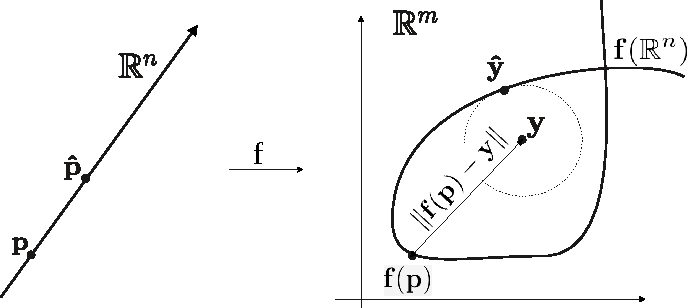
\includegraphics[width=9cm]{moindrecarre}\caption{Illustration of the least squares method in the nonlinear case}

\label{fig:moindrecarre}
\end{figure}

When $\mathbf{f}(\mathbf{p})$ is nonlinear, we can use a local optimization
algorithm to try to obtain $\mathbf{\hat{p}}$. We propose now two
different approaches to perform a local minimization: the Newton method
and the Monte-Carlo algorithm.

\textbf{Newton Method}. In order to minimize $j(\mathbf{p})=||\mathbf{f}\left(\mathbf{\mathbf{p}}\right)-\mathbf{y}||^{2},$
the Newton method assumes that an approximation $\mathbf{p}_{0}$
of the minimizer is available. Around $\mathbf{p}_{0}$, we have:
\[
\mathbf{f}\left(\mathbf{\mathbf{p}}\right)\simeq\mathbf{f}\left(\mathbf{p}_{0}\right)+\frac{d\mathbf{f}}{d\mathbf{p}}(\mathbf{p}_{0})\cdot(\mathbf{p}-\mathbf{p}_{0}).
\]
Therefore
\[
\begin{array}{clcl}
j(\mathbf{p}) & = & \, & ||\mathbf{f}\left(\mathbf{\mathbf{p}}\right)-\mathbf{y}||^{2}\\
 & \simeq &  & ||\mathbf{f}\left(\mathbf{p}_{0}\right)+\underset{=\mathbf{M}}{\underbrace{\frac{d\mathbf{f}}{d\mathbf{p}}(\mathbf{p}_{0})}}\cdot(\mathbf{p}-\mathbf{p}_{0})-\mathbf{y}||^{2}\\
 & = &  & ||\mathbf{M}\cdot\mathbf{p}+\underset{=-\mathbf{z}}{\underbrace{\mathbf{f}\left(\mathbf{p}_{0}\right)-\mathbf{M}\cdot\mathbf{p}_{0}-\mathbf{y}}}||^{2}\\
 & = &  & ||\mathbf{M}\cdot\mathbf{p}-\mathbf{z}||^{2}
\end{array}
\]
The minimizer is 
\[
\begin{array}{cccl}
\mathbf{p}_{1} & = & \, & \underset{=\mathbf{K}}{\underbrace{\left(\mathbf{M}^{\text{T}}\mathbf{M}\right)^{-1}\mathbf{M}^{\text{T}}}}\cdot\mathbf{z}\\
 & = &  & \mathbf{K}\cdot(\mathbf{y}-\mathbf{f}\left(\mathbf{p}_{0}\right)+\mathbf{M}\cdot\mathbf{p}_{0})\\
 & = &  & \mathbf{p}_{0}+\mathbf{K}\cdot(\mathbf{y}-\mathbf{f}(\mathbf{p}_{0}))
\end{array}
\]
which is expected to be closer to the solution than $\mathbf{p}_{0}$.
We apply the procedure several times and we get the following Newton
algorithm.

\begin{singlespace}
\begin{center}
\begin{tabular}{|cl|}
\hline 
 & $\textbf{Algorithm}\ensuremath{\;}\textsc{Newton }(\text{in}:\mathbf{p}_{0},\mathbf{y})$\tabularnewline
\hline 
1 & for $k=0$ to $k_{max}$\tabularnewline
2 & \hspace{1cm}$\mathbf{M}=\frac{d\mathbf{f}}{d\mathbf{p}}(\mathbf{p}_{k})$~\tabularnewline
3 & \hspace{1cm}$\mathbf{K}=\left(\mathbf{M}^{\text{T}}\mathbf{M}\right)^{-1}\mathbf{M}^{\text{T}}$\tabularnewline
4 & \hspace{1cm}$\mathbf{p}_{k+1}=\mathbf{p}_{k}+\mathbf{K}\cdot(\mathbf{y}-\mathbf{f}(\mathbf{p}_{k}))$\tabularnewline
\hline 
\end{tabular}
\par\end{center}
\end{singlespace}

The Newton algorithm is illustrated by Figure \ref{fig:newtonmin}.
In the left figure, the sequence is represented on the $\mathbf{p\text{-}y}$
space. We observe that we converge to the point $\hat{\mathbf{p}}$
which satisfies $\mathbf{f}(\hat{\mathbf{p}})=\mathbf{y}$ but this
is mainly due to the fact that we have a two dimensional representation.
In practice we only have $||\mathbf{f}\left(\mathbf{\mathbf{p}}\right)-\mathbf{y}||^{2}\simeq0$.
On the right figure, the representation is made on the $\mathbf{p}\text{-}j$
space. 

Unfortunately, even if the solution of our minimization problem is
unique, the Newton algorithm may diverge or converge to a point which
is not the solution of our problem.

\begin{figure}[H]
\centering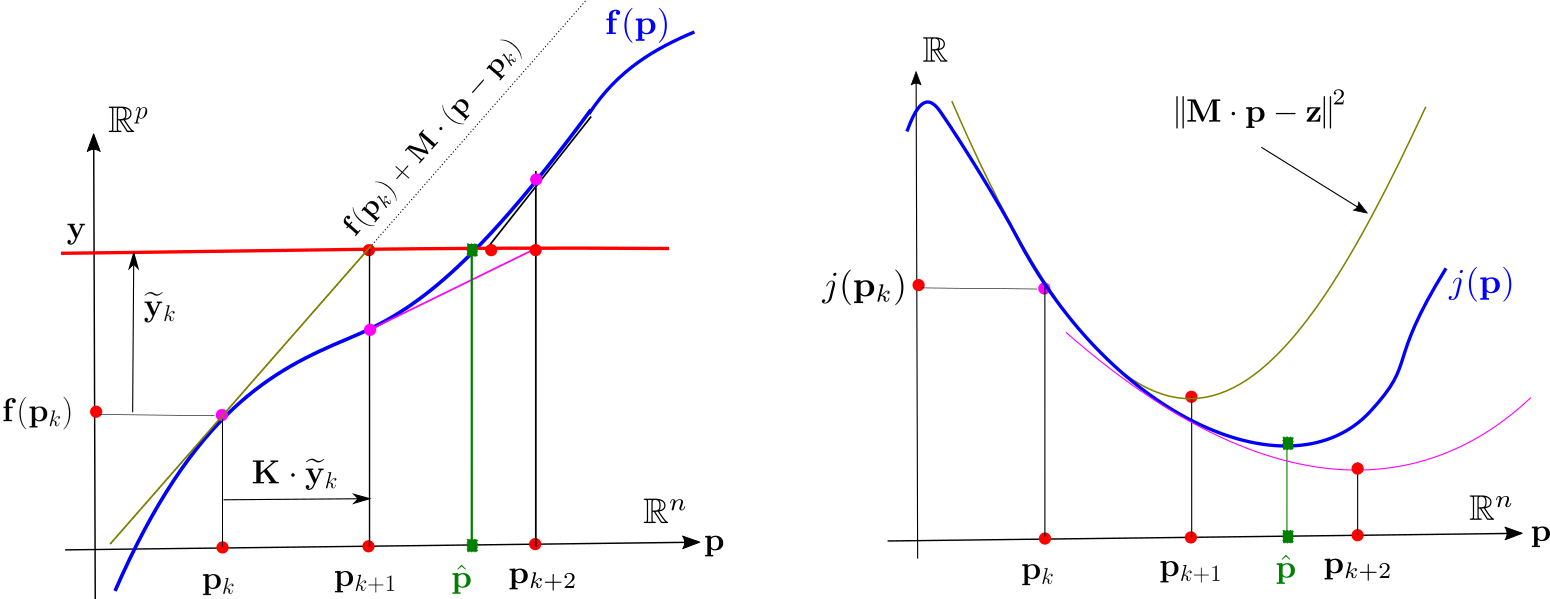
\includegraphics[width=13cm]{newton_min}\caption{Illustration of the Newton method to minimize $||\mathbf{f}(\mathbf{p})-\mathbf{y}||^{2}$ }

\label{fig:newtonmin}
\end{figure}

\textbf{Monte-Carlo method}. The algorithm below proposes a simple
version of a Monte-Carlo algorithm:

\begin{singlespace}
\begin{center}
\begin{tabular}{|cl|}
\hline 
 & $\textbf{Algorithm}\ensuremath{\;}\textsc{Minimize}(\text{input: }\ensuremath{\mathbf{p}})$\tabularnewline
\hline 
1 & take a random movement $\mathbf{d}$\tabularnewline
2 & $\ensuremath{\mathbf{q}=\mathbf{p}+\mathbf{d}}$\tabularnewline
3 & $\mbox{if }\ensuremath{j\left(\mathbf{q}\right)<j(\mathbf{p})}\mbox{ then }\ensuremath{\mathbf{p}=\mathbf{q}}$\tabularnewline
4 & go to 1\tabularnewline
\hline 
\end{tabular}
\par\end{center}
\end{singlespace}

Again, this algorithm is expected to converge toward a local optimum
of the criterion $j(\mathbf{p})=||\mathbf{f}(\mathbf{p})-\mathbf{y}||^{2}$.
The quantity $\mathbf{d}$ is the step that represents a small vector
taken randomly from $\mathbb{R}^{n}$. In the case of the \emph{simulated
annealing} method, the amplitude of this step decreases with the iterations
in function of a parameter called \emph{temperature} which decreases
with time. If the initial temperature, is high enough and if the temperature
decreases sufficiently slowly, then we generally converge to the global
minimum.

\chapter*{Exercises}

\begin{Exercice} \label{ex:newton}Newton method for localization
\end{Exercice}

\textcolor{blue}{See the correction video at \href{https://youtu.be/f4ID4iyEEZc}{https://youtu.be/f4ID4iyEEZc}}

We consider a robot which is at unknown position\textbf{ $\mathbf{p}=(p_{1},p_{2})$}.
It measures distances to $4$ landmarks at position
\[
\mathbf{m}(1)=\left(\begin{array}{c}
-1\\
1
\end{array}\right),\,\mathbf{m}(2)=\left(\begin{array}{c}
1\\
2
\end{array}\right),\,\,\mathbf{m}(3)=\left(\begin{array}{c}
3\\
2
\end{array}\right),\,\,\mathbf{m}(4)=\left(\begin{array}{c}
4\\
5
\end{array}\right).
\]
as illustrated by Figure \ref{fig:newton_loc}. 

1) Assume that the robot is at position $\mathbf{p}$, give an expression
for the vector $\mathbf{f}(\mathbf{p})\in\mathbb{R}^{4}$ of all distances
to the landmarks. Compute $\mathbf{f}(\mathbf{p})$ for $\mathbf{p}=(2,-3)$.

\begin{figure}[H]
\centering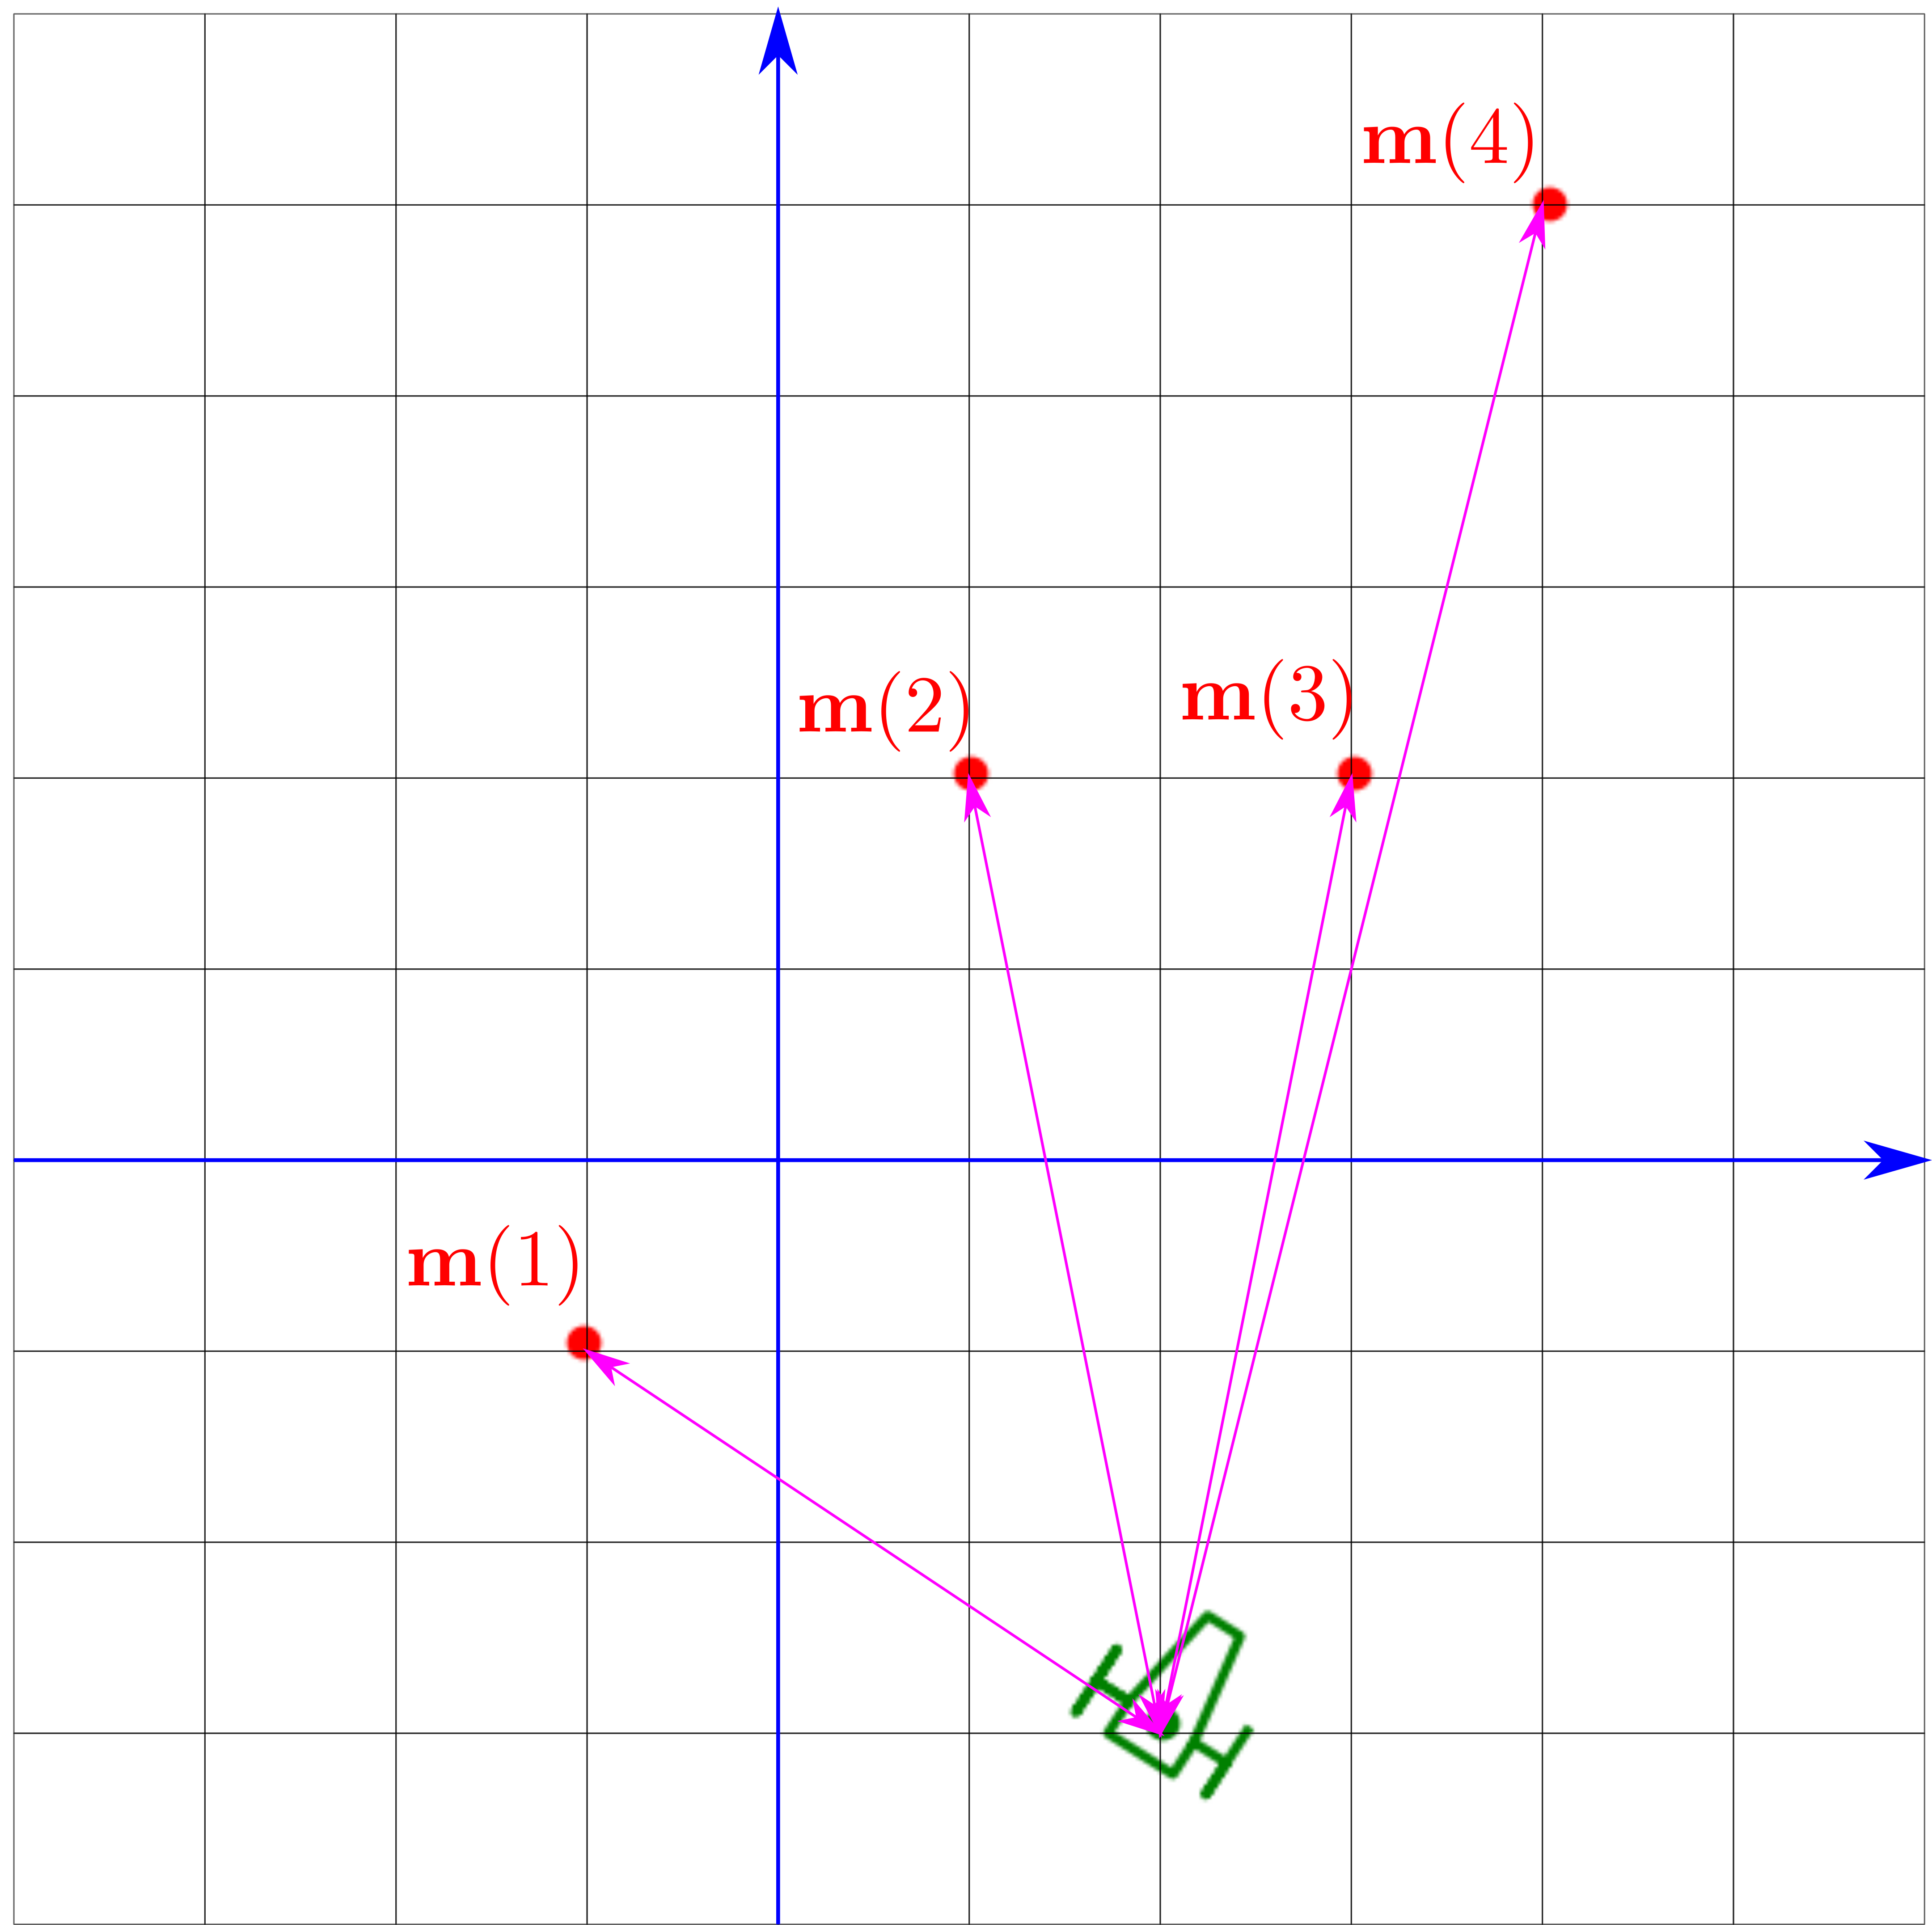
\includegraphics[width=7cm]{newton_loc}\caption{The robot measures the distances to the four landmarks}

\label{fig:newton_loc}
\end{figure}

2) Assume that the distance to the landmarks that have been measured
are given by the vector 
\[
\mathbf{y}=(4,5,5,8).
\]
To estimate the position of the robot, we propose to use a least-square
approach. For this, we build the criterion
\[
j(\mathbf{p})=\|\mathbf{f}(\mathbf{p})-\mathbf{y}\|^{2}.
\]
Draw the level curves for $j(\mathbf{p})$. Discuss.

3) Using a Newton minimization method, provide a least-square estimation
of $\mathbf{p}$. The initial point will be chosen as $\mathbf{p}(\text{0)=}(4,3).$

\rule{0.95\columnwidth}{1pt}

\begin{Exercice} \label{ex:montecarlo}Monte-Carlo method \end{Exercice}

\textcolor{blue}{See the correction video at \href{https://youtu.be/K6PeWq1AYwM}{https://youtu.be/K6PeWq1AYwM}}

Consider the discrete-time system given by its state representation:
\[
\left\{ \begin{array}{ccccccc}
\mathbf{x}(k+1) & = & \left(\begin{array}{ccc}
1 &  & 0\\
a &  & 0.3
\end{array}\right) & \mathbf{x}(k) & + & \left(\begin{array}{c}
b\\
1-b
\end{array}\right) & u(k)\\
y(k) & = & \left(\begin{array}{lcl}
1 & \,\, & 1\end{array}\right) & \mathbf{x}(k)
\end{array}\right.
\]
where $a,b$ are two parameters to be estimated. The initial state
is given by $\mathbf{x}(0)=(0,0)$ and $u(k)=1.$ We collect six measurements:
\[
\left(y(0),\cdots,y(5)\right)=\left(\begin{array}{llllll}
0, & 1, & 2.5, & 4.1, & 5.8, & 7.5\end{array}\right).
\]
Let us note that these values were obtained for the values $a^{\ast}=0.9$
and $b^{\ast}=0.75$, but we are not supposed to know them. We will
only assume that $a\in\left[0,2\right]$ and $b\in\left[0,2\right].$

1) Write a program that estimates the parameters $a$ and $b$ using
a Monte Carlo method. For this, generate a cloud of vectors $\mathbf{p}=(a,b)$
using a uniform random law. Then, by simulating the state equations,
calculate for all the $\mathbf{p}$ the corresponding outputs $y_{m}(\mathbf{p,}k)$.
Draw on the screen the vectors $\mathbf{p}$ such that for each $k\in\{0,\dots,5\}$,
$|y_{m}(k)-y(k)|<\varepsilon$, where $\varepsilon$ is a small positive
number.

2) Calculate the transfer function of the system in function of $a$
and $b$.

3) Let us assume that the real values $a^{\ast}=0.9$ and $b^{\ast}=0.75$
for $a$ and $b$ are known. Calculate the set of all pairs $\left(a,b\right)$
that generate the same transfer function as the pair $(a^{\ast},b^{\ast})$.
Deduce from this an interpretation of the results obtained in question
1).

\rule{0.95\columnwidth}{1pt}

\begin{Exercice} \label{ex:recuit} Localization by simulated annealing
\index{localization}\end{Exercice}

\textcolor{blue}{See the correction video at \href{https://youtu.be/oHbTrxpnOHo}{https://youtu.be/oHbTrxpnOHo}}

The localization problem that we will now consider is inspired from
\cite{Jaulin02Robab}. The robot, represented on Figure \ref{fig:robot:telem:laser},
is equipped with eight laser telemeters\index{telemeter} capable
of measuring its distance from the walls for angles equal to $\frac{k\pi}{4}$,
$k\in\{0,\dots,7\}$. We assume that the obstacles are composed of
$n$ segments $\left[\mathbf{a}_{i}\mathbf{b}_{i}\right],$ $i=1,\dots,n$,
where the coordinates of $\mathbf{a}_{i}$ and $\mathbf{b}_{i}$ are
known. The eight distances are stored in the vector $\mathbf{y}$
and the localization problem amounts to estimating the position and
orientation of the robot from $\mathbf{y}$.

\begin{figure}[H]
\centering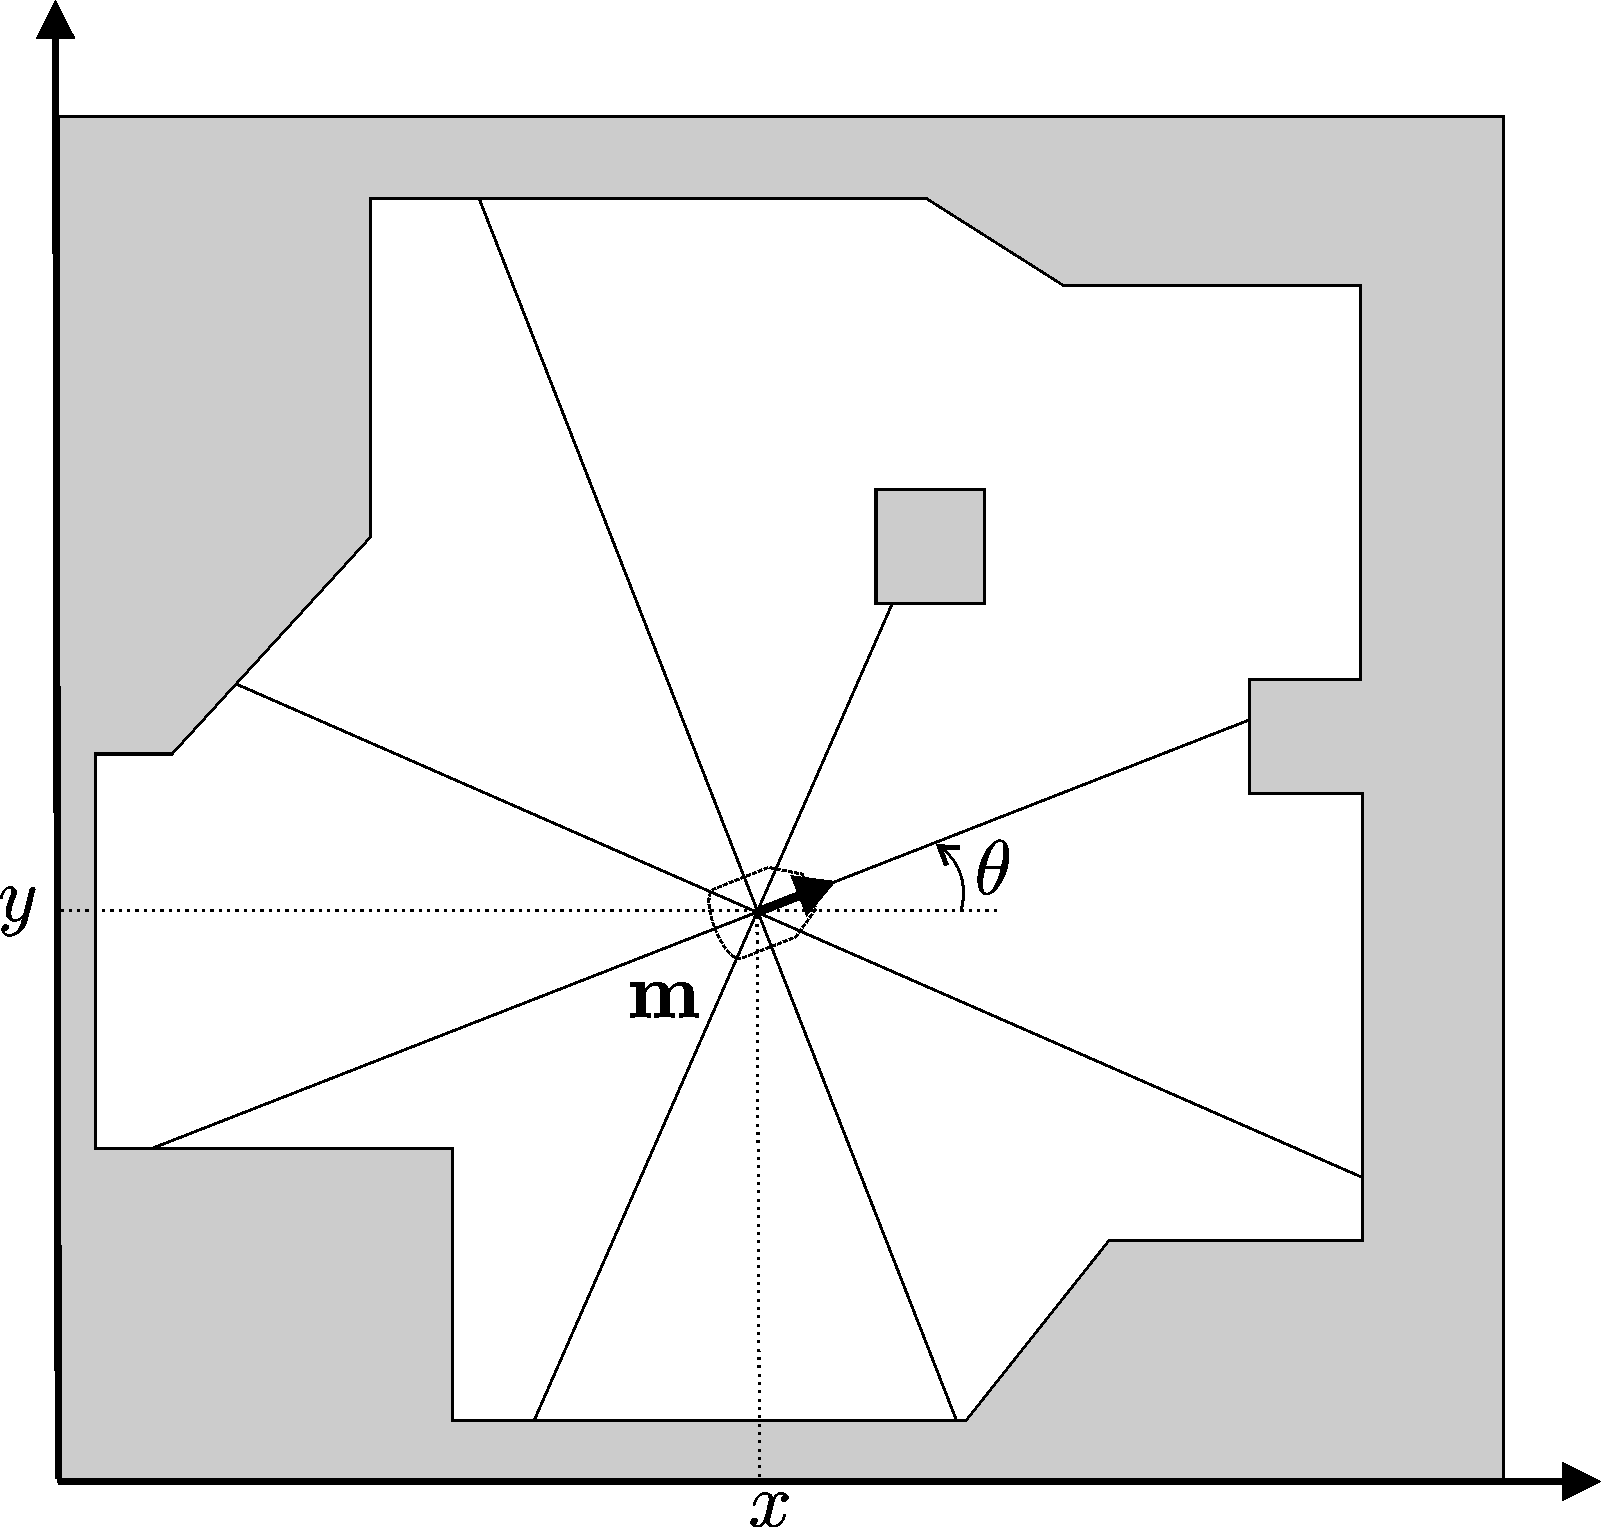
\includegraphics[width=7cm]{robot_hokuyo}\caption{Robot equipped with eight telemeters trying to localize itself}

\label{fig:robot:telem:laser}
\end{figure}

1)\textbf{\ }Let $\mathbf{m}$,\textbf{\ }$\mathbf{a}$,\textbf{\ }$\mathbf{b}$
be three points of $\mathbb{R}^{2}$ and $\overrightarrow{\mathbf{u}}$
a unit vector. Show that the ray $\mathcal{E}\left(\mathbf{m,}\overrightarrow{\mathbf{u}}\right)$
intersects the segment $\left[\mathbf{ab}\right]$ if and only if:
\[
\left\{ \begin{array}{cc}
\det\left(\mathbf{a}-\mathbf{m},\overrightarrow{\mathbf{u}}\right)\cdot\det\left(\mathbf{b}-\mathbf{m},\overrightarrow{\mathbf{u}}\right) & \leq0\\
\det(\mathbf{a}-\mathbf{m},\mathbf{b}-\mathbf{a})\cdot\det(\overrightarrow{\mathbf{u}},\mathbf{b}-\mathbf{a}) & \geq0
\end{array}\right.
\]
If this condition is verified, show that the distance from $\mathbf{m}$
to $\left[\mathbf{ab}\right]$ following $\overrightarrow{\mathbf{u}}$
is: 
\[
d=\frac{\det(\mathbf{a}-\mathbf{m},\mathbf{b}-\mathbf{a})}{\det(\overrightarrow{\mathbf{u}},\mathbf{b}-\mathbf{a})}.
\]

2) Design a simulator $\mathbf{f}\left(\mathbf{p}\right)$ that calculates
the directional distances between the pose $\mathbf{p}=\left(x,y,\theta\right)$
and the walls.
\begin{flushleft}
3) Using a global simulated annealing-type optimization method, design
a program that gives a least squares estimation $\mathbf{\hat{p}}$
of the pose $\mathbf{p}$ from $\mathbf{y}$. For the segments $\left[\mathbf{a}_{i},\mathbf{b}_{i}\right]$
of the room and for the vector of the measured distances, take the
following quantities:
\[
\begin{array}{ccc}
\mathbf{A} & = & \left(\begin{array}{ccccccccccccccccccccccccccc}
0 &  & 7 &  & 7 &  & 9 &  & 9 &  & 7 &  & 7 &  & 4 &  & 2 &  & 0 &  & 5 &  & 6 &  & 6 &  & 5\\
0 &  & 0 &  & 2 &  & 2 &  & 4 &  & 4 &  & 7 &  & 7 &  & 5 &  & 5 &  & 2 &  & 2 &  & 3 &  & 3
\end{array}\right)\\
\mathbf{B} & = & \left(\begin{array}{ccccccccccccccccccccccccccc}
7 &  & 7 &  & 9 &  & 9 &  & 7 &  & 7 &  & 4 &  & 2 &  & 0 &  & 0 &  & 6 &  & 6 &  & 5 &  & 5\\
0 &  & 2 &  & 2 &  & 4 &  & 4 &  & 7 &  & 7 &  & 5 &  & 5 &  & 0 &  & 2 &  & 3 &  & 3 &  & 2
\end{array}\right)\\
\mathbf{y} & = & \left(6.4,\,3.6,\,2.3,\,2.1,\,1.7,\,1.6,\,3.0,\,3.1\right)^{\text{T}}
\end{array}
\]
\par\end{flushleft}


\chapter{Covariance matrices\label{sst:kalman:cov-1}}

The Kalman filter is mainly based on the concept of covariance matrix
which is important to grasp in order to understand the design and
the utilization of the observer. This section recalls the fundamental
concepts surrounding covariance matrices.

\section{Definitions and interpretations\label{sst:kalman:cov:interpret}}

Let us consider two random vectors $\mathbf{x}\in\mathbb{R}^{n}$
and $\mathbf{y}\in\mathbb{R}^{m}$. The mathematical expectations
of $\mathbf{x}$ and $\mathbf{y}$ are denoted by $\mathbf{\bar{x}}=E\left(\mathbf{x}\right)$,
$\mathbf{\bar{y}}=E\left(\mathbf{y}\right)$. Let us define the \emph{variations}
of $\mathbf{x}$ and $\mathbf{y}$ by $\widetilde{\mathbf{x}}=\mathbf{x}-\mathbf{\bar{x}}$
and $\widetilde{\mathbf{y}}=\mathbf{y}-\mathbf{\bar{y}}$. The \emph{covariance
matrix} is given by: 
\[
\mathbf{\boldsymbol{\Gamma}}_{\mathbf{xy}}=E\left(\widetilde{\mathbf{x}}\cdot\widetilde{\mathbf{y}}^{\text{T}}\right)=E\left(\left(\mathbf{x}-\mathbf{\bar{x}}\right)\left(\mathbf{y}-\mathbf{\bar{y}}\right)^{\text{T}}\right).
\]
The covariance matrix for $\mathbf{x}$ is defined by: 
\[
\mathbf{\boldsymbol{\Gamma}}_{\mathbf{x}}=\mathbf{\boldsymbol{\Gamma}}_{\mathbf{xx}}=E\left(\widetilde{\mathbf{x}}\cdot\widetilde{\mathbf{x}}^{\text{T}}\right)=E\left(\left(\mathbf{x}-\mathbf{\bar{x}}\right)\left(\mathbf{x}-\mathbf{\bar{x}}\right)^{\text{T}}\right).
\]
The one for $\mathbf{y}$ is: 
\[
\mathbf{\boldsymbol{\Gamma}}_{\mathbf{y}}=\mathbf{\boldsymbol{\Gamma}}_{\mathbf{yy}}=E\left(\widetilde{\mathbf{y}}\cdot\widetilde{\mathbf{y}}^{\text{T}}\right)=E\left(\left(\mathbf{y}-\mathbf{\bar{y}}\right)\left(\mathbf{y}-\mathbf{\bar{y}}\right)^{\text{T}}\right).
\]
Let us note that $\mathbf{x}$, $\mathbf{y}$, $\widetilde{\mathbf{x}}$,
$\widetilde{\mathbf{y}}$ are random vectors whereas $\mathbf{\bar{x}},\mathbf{\bar{y}},\mathbf{\boldsymbol{\Gamma}}_{\mathbf{x}},\mathbf{\boldsymbol{\Gamma}}_{\mathbf{y}},\mathbf{\boldsymbol{\Gamma}}_{\mathbf{xy}}$
are deterministic. A covariance matrix $\mathbf{\boldsymbol{\Gamma}}_{\mathbf{x}}$
of a random vector $\mathbf{x}$ is always positive definite (we will
write $\mathbf{\boldsymbol{\Gamma}}_{\mathbf{x}}\succ\mathbf{0}$),
except in the degenerate case. In a computer, a random vector can
be represented by a cloud of points associated with realizations.
Let us consider the following program:
\begin{singlespace}
\begin{center}
\begin{tabular}{|cl|}
\hline 
1 & $N:=1000;\,\mathbf{x}:=2\cdot\mathbf{1}_{N\times1}+\text{randn}_{N\times1}\,$\tabularnewline
2 & $\mathbf{y}:=2\cdot\left(\begin{array}{c}
x_{1}^{2}\\
\vdots\\
x_{N}^{2}
\end{array}\right)+\text{randn}_{N\times1}$\tabularnewline
3 & $\bar{x}:=\frac{1}{N}\sum_{i}x_{i};\,\,\,\bar{y}=\frac{1}{N}\sum_{i}y_{i}$\tabularnewline
4 & $\widetilde{\mathbf{x}}:=\mathbf{x}-\bar{x}\cdot\mathbf{1}_{N\times1};\widetilde{\mathbf{y}}=\mathbf{y}-\bar{y}\cdot\mathbf{1}_{N\times1}\,$\tabularnewline
5 & $\left(\begin{array}{cc}
\Gamma_{x} & \Gamma_{xy}\\
\Gamma_{xy} & \Gamma_{y}
\end{array}\right):=\frac{1}{N}\cdot\left(\begin{array}{cc}
\sum_{i}\widetilde{x}_{i}^{2} & \sum_{i}\widetilde{x}_{i}\widetilde{y}_{i}\\
\sum_{i}\widetilde{x}_{i}\widetilde{y}_{i} & \sum_{i}\widetilde{y}_{i}^{2}
\end{array}\right)$\tabularnewline
\hline 
\end{tabular}
\par\end{center}
\end{singlespace}

This yields Figure\ \ref{fig:kalman:cov}, which gives us a representation
of the random variables $x,y$ (on the left) and of $\widetilde{x},\widetilde{y}$
(on the right). The program also gives us the estimations: 
\[
\bar{x}\simeq1.99,\bar{y}\simeq9.983,\Gamma_{x}\simeq1.003,\Gamma_{y}\simeq74.03,\Gamma_{xy}\simeq8.082.
\]

\begin{figure}[H]
\centering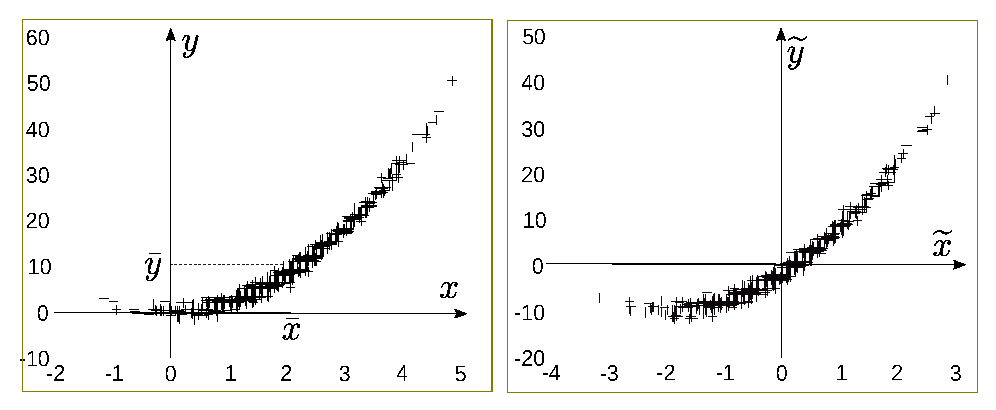
\includegraphics[width=12cm]{kalman_cov}\caption{Cloud of points that represents a pair of two random variables}

\label{fig:kalman:cov}
\end{figure}

Two random vectors $\mathbf{x}$ and $\mathbf{y}$ are linearly independent
(or non-correlated or orthogonal) if $\mathbf{\boldsymbol{\Gamma}}_{\mathbf{xy}}=\mathbf{0}$.
On Figure \ref{fig:kalman:indep}, the two clouds of points correspond
to non-correlated variables. Only the figure on the right corresponds
to independent variables.

\begin{figure}[H]
\centering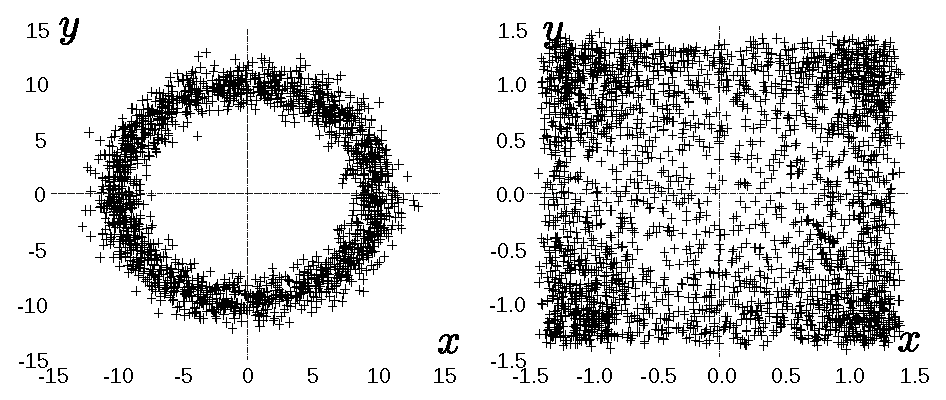
\includegraphics[width=12cm]{kalman_indep}\caption{Left : dependent but non-correlated variables $\left(x,y\right)$
; Right : independent variables}

\label{fig:kalman:indep}
\end{figure}

The figure on the left was generated by:
\begin{singlespace}
\begin{center}
\begin{tabular}{|cl|}
\hline 
1 & $N:=2000;\,\,$\tabularnewline
2 & $\boldsymbol{\rho}:=10\cdot\mathbf{1}_{N\times1}+\text{randn}_{N\times1}$\tabularnewline
3 & $\boldsymbol{\theta}:=2\pi\cdot\text{rand}_{N\times1}$\tabularnewline
4 & $\mathbf{x}:=\left(\begin{array}{c}
\rho_{1}\sin\theta_{1}\\
\vdots\\
\rho_{N}\sin\theta_{N}
\end{array}\right)$;~$\mathbf{y}:=\left(\begin{array}{c}
\rho_{1}\cos\theta_{1}\\
\vdots\\
\rho_{N}\cos\theta_{N}
\end{array}\right)$\tabularnewline
\hline 
\end{tabular}
\par\end{center}
\end{singlespace}

And the figure on the right was generated by:
\begin{singlespace}
\begin{center}
\begin{tabular}{|cl|}
\hline 
1 & $N:=2000;\,\,$\tabularnewline
2 & $\mathbf{x}:=\text{atan\ensuremath{\left(2\cdot\text{randn}_{N\times1}\right)}}$\tabularnewline
3 & $\mathbf{y}:=\text{atan\ensuremath{\left(2\cdot\text{randn}_{N\times1}\right)}}$\tabularnewline
\hline 
\end{tabular}
\par\end{center}
\end{singlespace}

\textbf{Whiteness}\index{whiteness}. A random vector $\mathbf{x}$
is called \emph{white} if all of its components $x_{i}$ are independent
from one another. In such a case, the covariance vector $\boldsymbol{\Gamma}_{\mathbf{x}}$
of $\mathbf{x}$ is diagonal.

\section{Properties}

Covariance matrices are symmetric and positive, \emph{i.e.}, all of
their eigenvalues are real and positive. The set of all covariance
matrices of $\mathbb{R}^{n\times n}$ will be denoted by $\mathcal{S}^{+}\left(\mathbb{R}^{n}\right)$.

\textbf{Decomposition}. Every symmetric matrix $\mathbf{\boldsymbol{\Gamma}}$
can be put into a diagonal form and has an orthonormal eigenvector
basis. We may therefore write: 
\[
\mathbf{\boldsymbol{\Gamma}}=\mathbf{R}\cdot\mathbf{D}\cdot\mathbf{R}^{-1}
\]
where $\mathbf{R}$ is a rotation matrix (i.e. $\mathbf{R}^{\text{T}}\mathbf{R=I}$
and $\det\mathbf{R}=1$). The matrix $\mathbf{R}$ corresponds to
the eigenvectors and $\mathbf{D}$ is a diagonal matrix whose elements
are the eigenvalues. For the matrices of $\mathcal{S}^{+}\left(\mathbb{R}^{n}\right)$,
these eigenvalues are positive.

\textbf{Square root}. Every matrix $\mathbf{\boldsymbol{\Gamma}}$
of $\mathcal{S}^{+}\left(\mathbb{R}^{n}\right)$ has a square root
in $\mathcal{S}^{+}\left(\mathbb{R}^{n}\right)$. This square root
will be denoted by $\mathbf{\boldsymbol{\Gamma}}^{\frac{1}{2}}$.
Following the eigenvalue correspondence theorem, the eigenvalues of
$\mathbf{\boldsymbol{\Gamma}}^{\frac{1}{2}}$ are the square roots
of those of the eigenvalues of $\mathbf{\boldsymbol{\Gamma}}$.

\textbf{Example}. Consider the following script:
\begin{singlespace}
\begin{center}
\begin{tabular}{|cl|}
\hline 
1 & $\mathbf{A}:=\text{rand}_{3\times3};\,$$\mathbf{S}_{1}:=\mathbf{A}\cdot\mathbf{A}^{\text{T}}$\tabularnewline
2 & $[\mathbf{R},\mathbf{D}]:=\text{eig}(\mathbf{S}_{1})$; $\mathbf{S}_{2}:=\mathbf{R}\cdot\mathbf{D}\cdot\mathbf{R}^{\text{T}}$\tabularnewline
3 & $\mathbf{A}_{2}:=\mathbf{S}_{2}^{\frac{1}{2}};$~$\mathbf{S}_{3}:=\mathbf{A}_{2}\cdot\mathbf{A}_{2}^{\text{T}}$\tabularnewline
\hline 
\end{tabular}
\par\end{center}
\end{singlespace}

The matrix\texttt{ $\mathbf{D}$} is diagonal and the matrix\texttt{
$\mathbf{R}$} is a rotation matrix that contains the eigenvectors
of \texttt{$\mathbf{S}_{1}$}. The three matrices \texttt{$\mathbf{S}_{1},\mathbf{S}_{2},\mathbf{S}_{3}$}
are equal. This is not the case for matrices \texttt{$\mathbf{A}$}
and \texttt{$\mathbf{A}_{2}$} since only \texttt{$\mathbf{A}_{2}$}
is symmetric. Note that \texttt{$\mathbf{A}_{2}$} is a covariance
matrix.

\textbf{Order}. If $\mathbf{\boldsymbol{\Gamma}}_{1}$ and $\mathbf{\boldsymbol{\Gamma}}_{2}$
belong to $\mathcal{S}^{+}\left(\mathbb{R}^{n}\right)$, then $\mathbf{\boldsymbol{\Gamma}}=\alpha_{1}\mathbf{\boldsymbol{\Gamma}}_{1}+\alpha_{2}\mathbf{\boldsymbol{\Gamma}}_{2}$
also belongs to $\mathcal{S}^{+}\left(\mathbb{R}^{n}\right)$ if $\alpha_{1}\geq0$
and $\alpha_{2}\geq0$. This is equivalent to saying that $\mathcal{S}^{+}\left(\mathbb{R}^{n}\right)$
is a convex cone of $\mathbb{R}^{n\times n}$. Let us define the order
relation: 
\[
\mathbf{\boldsymbol{\Gamma}}_{1}\leq\mathbf{\boldsymbol{\Gamma}}_{2}\text{ }\Leftrightarrow\text{ }\mathbf{\boldsymbol{\Gamma}}_{2}-\mathbf{\boldsymbol{\Gamma}}_{1}\in\mathcal{S}^{+}\left(\mathbb{R}^{n}\right).
\]
It can be easily verified that it is reflexive, antisymmetric and
transitive. If $\mathbf{\boldsymbol{\Gamma}}_{1}\leq\mathbf{\boldsymbol{\Gamma}}_{2}$
then the $a$-level confidence ellipse (see following paragraph) of
$\mathbf{\boldsymbol{\Gamma}}_{1}$ is (in general) included in the
one that corresponds to $\mathbf{\boldsymbol{\Gamma}}_{2}$. The smaller
the covariance matrix (in the sense of this order relation), the more
precise it is. 

\section{Confidence ellipse\label{subsec:Confidence-ellipse}}

A random vector $\mathbf{x}$ of $\mathbb{R}^{n}$ can be characterized
by the pair $\left(\mathbf{\bar{x}},\mathbf{\boldsymbol{\Gamma}}_{\mathbf{x}}\right)$,
to which we can associate an ellipse of $\mathbb{R}^{n}$ which encloses
the consistent values for $\mathbf{x}$. In practice, for purely graphical
reasons, we often only look at two components $\mathbf{w}=\left(x_{i},x_{j}\right)$
of $\mathbf{x}$ (a computer screen is in fact two-dimensional). The
average $\mathbf{\bar{w}}$ can be directly deduced from $\mathbf{\bar{x}}$
by extracting the $i^{\text{th}}$ and $j^{\text{th}}$ components.
The covariance matrix $\mathbf{\boldsymbol{\Gamma}}_{\mathbf{w}}\in\mathcal{S}^{+}\left(\mathbb{R}^{2}\right)$
can also be obtained from $\mathbf{\boldsymbol{\Gamma}}_{\mathbf{x}}\in\mathcal{S}^{+}\left(\mathbb{R}^{n}\right)$
by extracting the $i^{\text{th}}$ and $j^{\text{th}}$ lines and
columns. The \emph{confidence ellipse} associated with $\mathbf{w}$
is described by the inequality: 
\[
\mathcal{E}_{\mathbf{w}}:\left(\mathbf{w}-\mathbf{\bar{w}}\right)^{\text{T}}\mathbf{\boldsymbol{\Gamma}}_{\mathbf{w}}^{-1}\left(\mathbf{w}-\mathbf{\bar{w}}\right)\leq a^{2}
\]
where $a$ is an arbitrary positive real number. Therefore if $\mathbf{w}$
is a Gaussian random vector, this ellipse corresponds to a contour
line of the probability density for $\mathbf{w}$. Since $\mathbf{\boldsymbol{\Gamma}}_{\mathbf{w}}^{-1}\succ\mathbf{0}$,
it has a square root $\mathbf{\boldsymbol{\Gamma}}_{\mathbf{w}}^{-\frac{1}{2}}$
which is also positive definite. We may therefore write: 
\[
\begin{array}{lll}
\mathcal{E}_{\mathbf{w}} & = & \left\{ \mathbf{w}\ |\ \left(\mathbf{w}-\mathbf{\bar{w}}\right)^{\text{T}}\ \mathbf{\boldsymbol{\Gamma}}_{\mathbf{w}}^{-\frac{1}{2}}\cdot\mathbf{\boldsymbol{\Gamma}}_{\mathbf{w}}^{-\frac{1}{2}}\left(\mathbf{w}-\mathbf{\bar{w}}\right)\leq a^{2}\right\} \\
 & = & \left\{ \mathbf{w}\ |\ \left\Vert \frac{1}{a}\cdot\mathbf{\boldsymbol{\Gamma}}_{\mathbf{w}}^{-\frac{1}{2}}\left(\mathbf{w}-\mathbf{\bar{w}}\right)\right\Vert \ \leq1\right\} \\
 & = & \left\{ \mathbf{w}\ |\ \frac{1}{a}\cdot\mathbf{\boldsymbol{\Gamma}}_{\mathbf{w}}^{-\frac{1}{2}}\left(\mathbf{w}-\mathbf{\bar{w}}\right)\ \in\mathcal{U}\right\} \text{, where }\mathcal{U}\text{ is the unit disk}\\
 & = & \left\{ \mathbf{w}\ |\ \mathbf{w}\ \in\mathbf{\bar{w}}+a\mathbf{\boldsymbol{\Gamma}}_{\mathbf{w}}^{\frac{1}{2}}\mathcal{U}\right\} \\
 & = & \mathbf{\bar{w}}+a\mathbf{\boldsymbol{\Gamma}}_{\mathbf{w}}^{\frac{1}{2}}\mathcal{U}.
\end{array}
\]
The ellipse $\mathcal{E}_{\mathbf{w}}$ can therefore be defined as
the image of the unit disk by the affine function $\mathbf{w}(\mathbf{s})=\mathbf{\bar{w}}+a\cdot\mathbf{\boldsymbol{\Gamma}}_{\mathbf{w}}^{\frac{1}{2}}\mathbf{\mathbf{s}}$,
as illustrated by Figure \ref{fig:confidence_ellip_circle}.

\begin{figure}[H]
\centering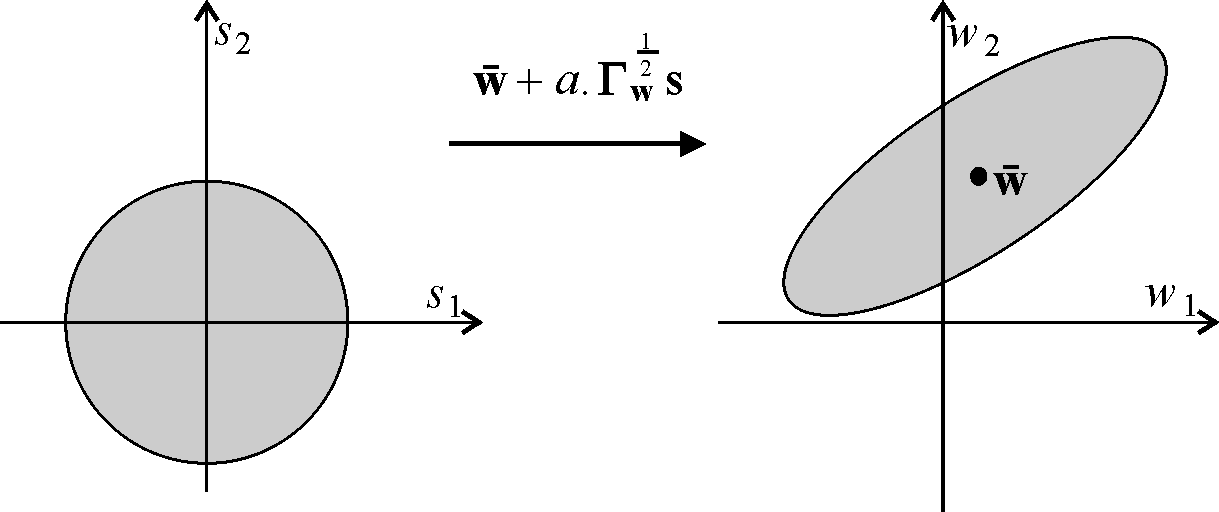
\includegraphics[width=11cm]{confidence_ellip_circle}\caption{A confidence ellipse is the image of the unit circle by an affine
function}

\label{fig:confidence_ellip_circle}
\end{figure}

Recall that for a centered, unit Gaussian random vector $\mathbf{s}$,
the random variable $z=\mathbf{s}^{\text{T}}\mathbf{s}$ follows a
$\chi^{2}$ law. In 2 dimensions, this probability density is given
by: 
\[
\pi_{z}(z)=\left\{ \begin{array}{c}
\frac{1}{2}\exp\left(-\frac{z}{2}\right)\text{ \ if\ \ }z\geq0\\
0\text{ otherwise}
\end{array}\right.
\]
Thus, for a given $a>0$, we have: 
\[
\begin{split}\eta\overset{\text{def}}{=}\text{prob}\left(||\mathbf{s||}\leq a\right)= & \text{prob}\left(\mathbf{s}^{\text{T}}\mathbf{s}\leq a^{2}\right)=\text{prob}\left(z\leq a^{2}\right)\\
= & \int_{0}^{a^{2}}\frac{1}{2}\exp\left(-\frac{z}{2}\right)dz=1-e^{-\frac{1}{2}a^{2}}.
\end{split}
\]
And therefore: 
\[
a=\sqrt{-2\ln\left(1-\eta\right)}.
\]
This relation allows us to calculate the threshold $a$ that we need
to choose in order to have a probability of being in the ellipse of
$\eta$. But careful, this probabilistic interpretation only makes
sense in the Gaussian case. The following function draws $\mathcal{E}_{\mathbf{w}}$
for a given probability $\eta$.
\begin{singlespace}
\begin{center}
\begin{tabular}{|cl|}
\hline 
 & $\textbf{Function}\ensuremath{\;}\textsc{DrawEllipse }(\bar{\mathbf{w}},\mathbf{\boldsymbol{\Gamma}}_{\mathbf{w}},\eta)$\tabularnewline
\hline 
1 & $\mathbf{w}=\bar{\mathbf{w}}+\sqrt{-2\ln\left(1-\eta\right)}\cdot\mathbf{\boldsymbol{\Gamma}}_{\mathbf{w}}^{\frac{1}{2}}\cdot\left(\begin{array}{ccccccc}
\cos0 &  & \cos0.1 &  & \cdots &  & \cos2\pi\\
\sin0 &  & \sin0.1 &  & \cdots &  & \sin2\pi
\end{array}\right)$\tabularnewline
2 & plot$(\mathbf{w})$\tabularnewline
\hline 
\end{tabular}
\par\end{center}
\end{singlespace}

\section{Generating Gaussian random vectors}

If we generate $n$ centered Gaussian random numbers, we obtain the
realization of a random vector whose center is $\mathbf{\bar{x}=0}$
and whose covariance matrix $\mathbf{\boldsymbol{\Gamma}}_{\mathbf{x}}\ $is
the identity matrix. In this section we will show, given a centered
Gaussian random number generator allowing us to realize $\mathbf{x}$,
how we can obtain a Gaussian random vector $\mathbf{y}$ of dimension
$n$ with an expectation and covariance matrix $\mathbf{\boldsymbol{\Gamma}}_{\mathbf{y}}$.
The main principle of this generation is based on the following theorem.
\begin{thm}
If $\mathbf{x},\mathbf{\boldsymbol{\alpha}}$ and $\mathbf{y}$ are
three random vectors connected by the relation $\mathbf{y}=\mathbf{Ax+\boldsymbol{\alpha}}+\mathbf{b}$
(where $\mathbf{A}$ and $\mathbf{b}$ are deterministic), and assuming
that $\mathbf{x},\mathbf{\boldsymbol{\alpha}}$ are independent and
that $\mathbf{\boldsymbol{\alpha}}$ is centered, we have: 
\begin{equation}
\begin{array}{lll}
\mathbf{\bar{y}} & = & \mathbf{A\bar{x}}+\mathbf{b}\\
\mathbf{\boldsymbol{\Gamma}}_{\mathbf{y}} & = & \mathbf{A}\cdot\mathbf{\boldsymbol{\Gamma}}_{\mathbf{x}}\cdot\mathbf{A}^{\text{T}}+\mathbf{\boldsymbol{\Gamma}}_{\mathbf{\boldsymbol{\alpha}}}
\end{array}\label{eq:matcov:linear}
\end{equation}
\end{thm}
\begin{proof}
\noindent We have: 
\[
\mathbf{\bar{y}}=E\left(\mathbf{Ax+\boldsymbol{\alpha}}+\mathbf{b}\right)=\mathbf{A}E\left(\mathbf{x}\right)+E\left(\mathbf{\boldsymbol{\alpha}}\right)+\mathbf{b}=\mathbf{A\bar{x}}+\mathbf{b}
\]
Moreover: 
\begin{align*}
\mathbf{\boldsymbol{\Gamma}}_{\mathbf{y}} & =E\left(\left(\mathbf{y}-\mathbf{\bar{y}}\right)\left(\mathbf{y}-\mathbf{\bar{y}}\right)^{\text{T}}\right)\\
 & =E\left(\left(\mathbf{Ax+\boldsymbol{\alpha}}+\mathbf{b}-\mathbf{A\bar{x}}-\mathbf{b}\right)\left(\mathbf{Ax+\boldsymbol{\alpha}}+\mathbf{b}-\mathbf{A\bar{x}}-\mathbf{b}\right)^{\text{T}}\right)\\
 & =E\left(\left(\mathbf{A}\widetilde{\mathbf{x}}+\mathbf{\boldsymbol{\alpha}}\right)\cdot\left(\mathbf{A}\widetilde{\mathbf{x}}+\mathbf{\boldsymbol{\alpha}}\right)^{\text{T}}\right)\\
 & =\mathbf{A}\cdot\underset{=\mathbf{\boldsymbol{\Gamma}}_{\mathbf{x}}}{\underbrace{E\left(\widetilde{\mathbf{x}}\cdot\widetilde{\mathbf{x}}^{\text{T}}\right)}}\cdot\mathbf{A}^{\text{T}}+\mathbf{A}\cdot\underset{=\mathbf{0}}{\underbrace{E\left(\widetilde{\mathbf{x}}\cdot\mathbf{\boldsymbol{\alpha}}^{\text{T}}\right)}}+\underset{=\mathbf{0}}{\underbrace{E\left(\mathbf{\boldsymbol{\alpha}}\cdot\widetilde{\mathbf{x}}^{\text{T}}\right)}}\cdot\mathbf{A}^{\text{T}}+\underset{=\mathbf{\boldsymbol{\Gamma}}_{\mathbf{\boldsymbol{\alpha}}}}{\underbrace{E\left(\mathbf{\boldsymbol{\alpha}}\cdot\mathbf{\boldsymbol{\alpha}}^{\text{T}}\right)}}\\
 & =\mathbf{A}\cdot\mathbf{\boldsymbol{\Gamma}}_{\mathbf{x}}\cdot\mathbf{A}^{\text{T}}+\mathbf{\boldsymbol{\Gamma}}_{\mathbf{\boldsymbol{\alpha}}}
\end{align*}
which concludes the proof.
\end{proof}
Thus, if $\mathbf{x}$ is a centered, unit Gaussian white random noise
(i.e. $\mathbf{\bar{x}=0}$ and $\mathbf{\mathbf{\boldsymbol{\Gamma}}}_{\mathbf{x}}=\mathbf{I}$),
and with $\boldsymbol{\alpha}=\mathbf{0}$ (i.e., $\mathbf{\boldsymbol{\Gamma}}_{\mathbf{\boldsymbol{\alpha}}}=\mathbf{0}$),
from (\ref{eq:matcov:linear}), we get
\[
\left\{ \begin{array}{ccc}
\mathbf{y} & = & \mathbf{Ax}+\mathbf{b}\\
\mathbf{\bar{y}} & = & \mathbf{b}\\
\mathbf{\boldsymbol{\Gamma}}_{\mathbf{y}} & = & \mathbf{A}\cdot\mathbf{A}^{\text{T}}
\end{array}\right.
\]
By choosing $\mathbf{A}=\mathbf{\boldsymbol{\Gamma}}_{\mathbf{y}}^{\frac{1}{2}}$
and $\mathbf{b}=\bar{\mathbf{y}}$, we get that the random vector
$\mathbf{y}=\mathbf{Ax}+\mathbf{b}$ will have an expectation of $\mathbf{\bar{y}}$
and a covariance matrix equal to $\mathbf{\boldsymbol{\Gamma}}_{\mathbf{y}}$
(see Figure \ref{fig:kalman_ellipse2}). To generate a Gaussian random
vector with covariance matrix $\mathbf{\boldsymbol{\Gamma}}_{\mathbf{y}}$
and expectation $\mathbf{\bar{y}}$, we will use this property. The
right side of Figure \ref{fig:kalman_ellipse2} was thus obtained
by the script:
\begin{singlespace}
\begin{center}
\begin{tabular}{|cl|}
\hline 
1 & $N:=1000;\,\,\mathbf{\boldsymbol{\Gamma}}_{\mathbf{y}}:=\left(\begin{array}{ccc}
3 &  & 1\\
1 &  & 3
\end{array}\right);\,\,\mathbf{\bar{y}}=\left(\begin{array}{c}
2\\
3
\end{array}\right);\,\,\mathbf{X}:=\text{randn}_{2\times n}$\tabularnewline
2 & $\mathbf{Y}:=\mathbf{\bar{y}}+\sqrt{\mathbf{\boldsymbol{\Gamma}}_{\mathbf{y}}}\cdot\mathbf{X}$\tabularnewline
3 & plot($\mathbf{Y}$)\tabularnewline
\hline 
\end{tabular}
\par\end{center}
\end{singlespace}

\begin{figure}[H]
\centering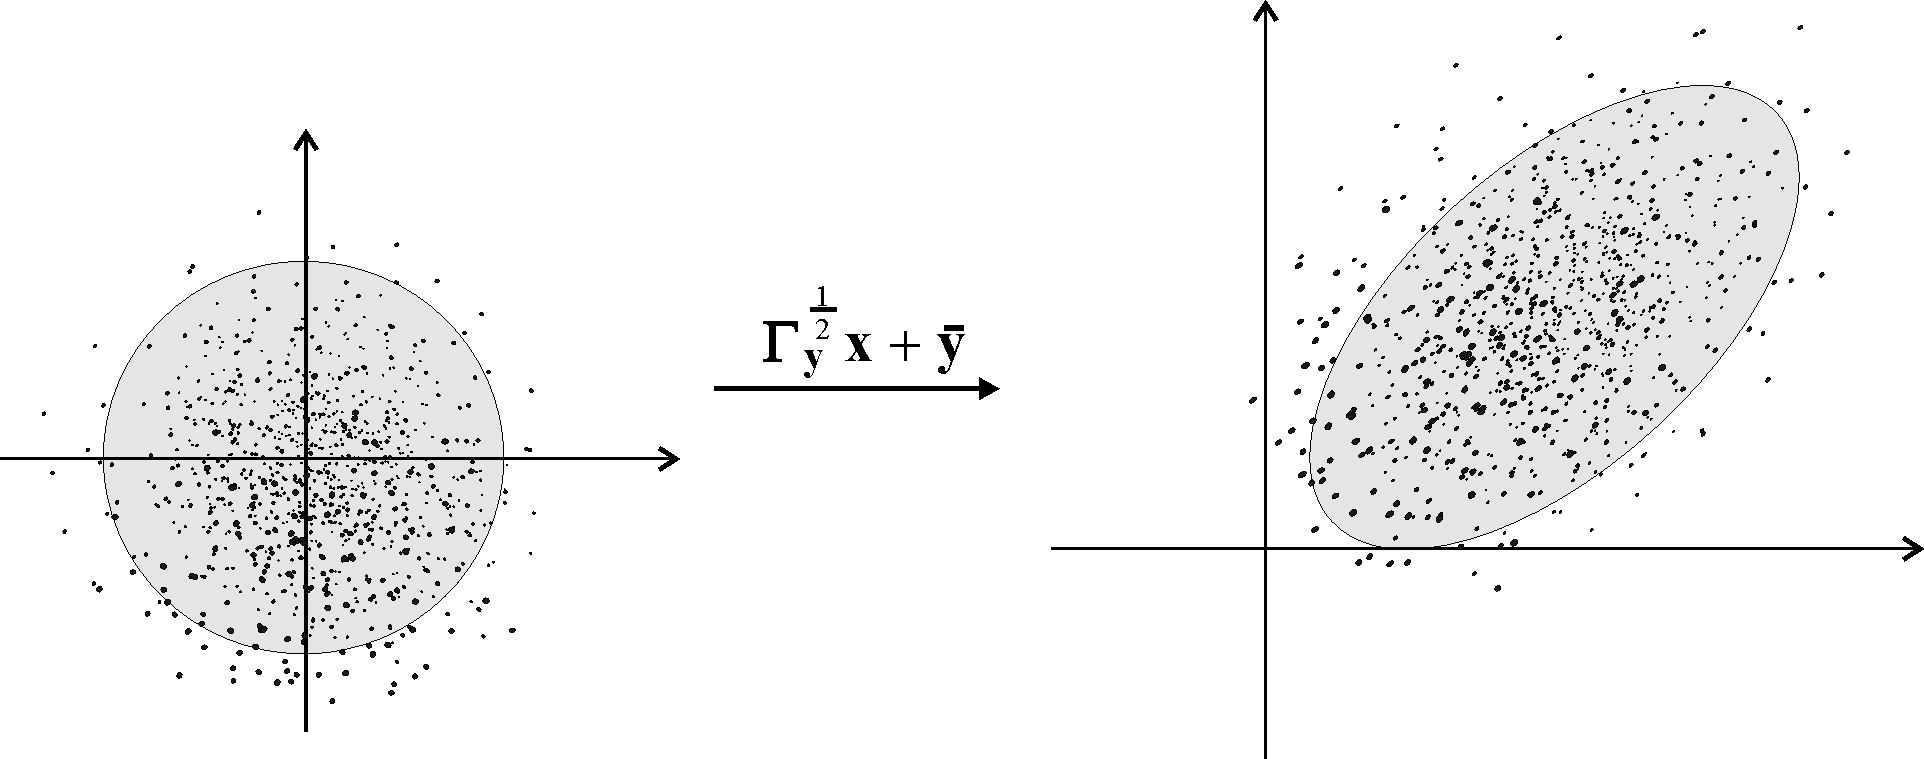
\includegraphics[width=13cm]{kalman_ellipse2} \caption{The Gaussian random vector $\mathbf{y}:\left(\mathbf{\bar{y}},\mathbf{\boldsymbol{\Gamma}}_{\mathbf{y}}\right)$
is the image by an affine application of a unit Gaussian white random
vector $\mathbf{x}$}

\label{fig:kalman_ellipse2}
\end{figure}


\chapter*{Exercises}

\begin{Exercice} \label{ex:distrib:gaussienne} Gaussian distribution
\end{Exercice}

\textcolor{blue}{See the correction video at \href{https://youtu.be/IZBcA8xzH0c}{https://youtu.be/IZBcA8xzH0c}}

The probability distribution of a random Gaussian vector $\mathbf{x}$
is fully characterized by its expectation $\mathbf{\bar{x}}$ and
its covariance matrix $\mathbf{\boldsymbol{\Gamma}}_{\mathbf{x}}$.
More precisely, it is given by: 
\[
\pi_{\mathbf{x}}(\mathbf{x})=\frac{1}{\sqrt{\left(2\pi\right)^{n}\det(\mathbf{\boldsymbol{\Gamma}}_{\mathbf{x}})}}\cdot\exp\left(-\frac{1}{2}\left(\mathbf{x}-\mathbf{\bar{x}}\right)^{\text{T}}\cdot\mathbf{\boldsymbol{\Gamma}}_{\mathbf{x}}^{-1}\cdot\left(\mathbf{x}-\mathbf{\bar{x}}\right)\right).
\]
1) Draw the graph and the contour lines of $\pi_{\mathbf{x}}$ with:
\[
\mathbf{\bar{x}}=\left(\begin{array}{c}
1\\
2
\end{array}\right)\text{ and }\mathbf{\boldsymbol{\Gamma}}_{\mathbf{x}}=\left(\begin{array}{ccc}
1 & \, & 0\\
0 &  & 1
\end{array}\right).
\]
2) We define the random vector: 
\[
\mathbf{y}=\left(\begin{array}{ccc}
\cos\frac{\pi}{6} &  & -\sin\frac{\pi}{6}\\
\sin\frac{\pi}{6} &  & \cos\frac{\pi}{6}
\end{array}\right)\left(\begin{array}{ccc}
1 & \, & 0\\
0 &  & 3
\end{array}\right)\mathbf{x}+\left(\begin{array}{c}
2\\
-5
\end{array}\right).
\]
Draw the graph and the contour lines of $\pi_{\mathbf{y}}$. Discuss.

\rule{0.95\columnwidth}{1pt}

\begin{Exercice} \label{ex:whoiswho:mat:cov} Confidence ellipses
\end{Exercice}

\textcolor{blue}{See the correction video at \href{https://youtu.be/jfQnFSmfKT8}{https://youtu.be/jfQnFSmfKT8}}

Let us generate six covariance matrices as follows:
\[
\begin{array}{lclcl}
\mathbf{A}_{1}=\left(\begin{array}{ccc}
1 &  & 0\\
0 &  & 3
\end{array}\right) & \,\, & \mathbf{A}_{2}=\left(\begin{array}{ccc}
\cos\frac{\pi}{4} &  & -\sin\frac{\pi}{4}\\
\sin\frac{\pi}{4} &  & \cos\frac{\pi}{4}
\end{array}\right) & \,\,\\
\boldsymbol{\Gamma}_{1}=\mathbf{I}_{2\times2} &  & \boldsymbol{\Gamma}_{2}=3\boldsymbol{\Gamma}_{1} &  & \boldsymbol{\Gamma}_{3}=\mathbf{A}_{1}\cdot\boldsymbol{\Gamma}_{2}\cdot\mathbf{A}_{1}^{\text{T}}+\boldsymbol{\Gamma}_{1}\\
\boldsymbol{\Gamma}_{4}=\mathbf{A}_{2}\cdot\boldsymbol{\Gamma}_{3}\cdot\mathbf{A}_{2}^{\text{T}} &  & \boldsymbol{\Gamma}_{5}=\boldsymbol{\Gamma}_{4}+\boldsymbol{\Gamma}_{3} &  & \boldsymbol{\Gamma}_{6}=\mathbf{A}_{2}\cdot\boldsymbol{\Gamma}_{5}\cdot\mathbf{A}_{2}^{\text{T}}
\end{array}
\]

Here,\texttt{ $\mathbf{A}_{2}$} corresponds to a rotation matrix
of angle $\frac{\pi}{4}$. Then, we draw the six confidence ellipses
at 90~\% associated with these matrices by centering them around
0. We thus obtain Figure \ref{fig:sixcov1}.

\begin{figure}[H]
\centering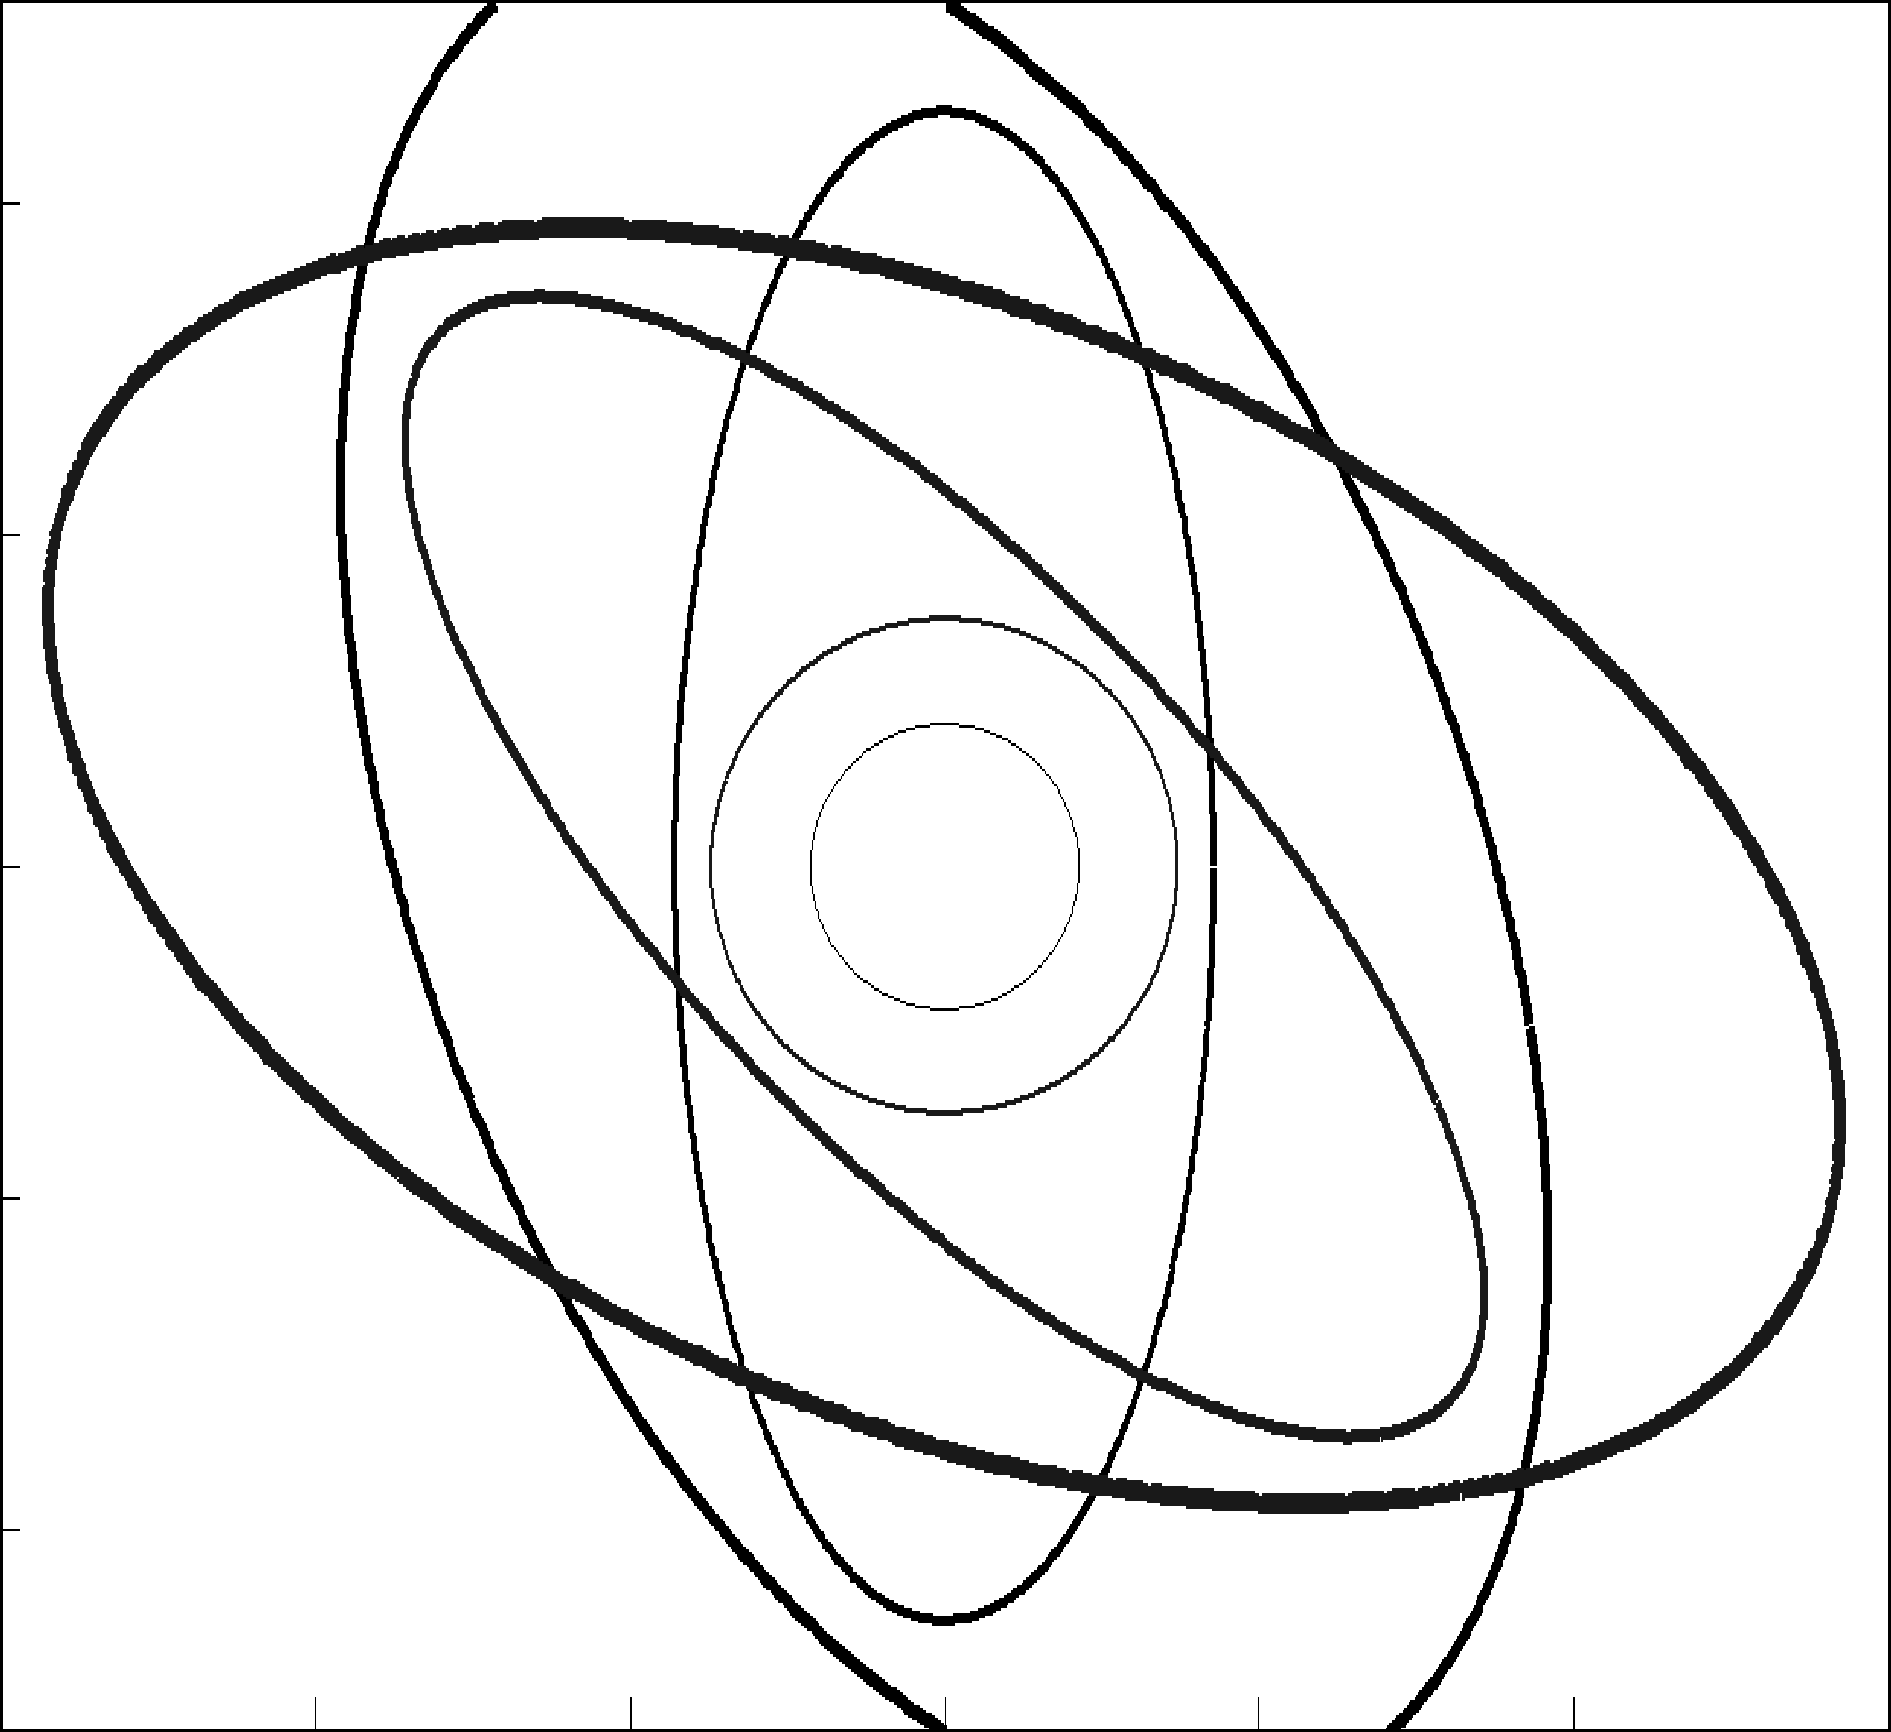
\includegraphics[width=6.8cm]{sixcov1}\caption{Confidence ellipses associated with the six covariance matrices}

\label{fig:sixcov1}
\end{figure}

1) Associate each covariance matrix with its confidence ellipse on
the figure.

2) Verify the result by regenerating these ellipses.

\rule{0.95\columnwidth}{1pt}

\begin{Exercice} \label{ex:ellipsoide:confiance:prediction} Confidence
ellipse: prediction \end{Exercice}

\textcolor{blue}{See the correction video at \href{https://youtu.be/yHG1GlvuZ7E}{https://youtu.be/yHG1GlvuZ7E}}

1) Generate a cloud of $N=1000$ points representing a random Gaussian
vector centered at $\mathbb{R}^{2}$ whose covariance matrix is the
identity matrix. Deduce from the latter a cloud of points for the
random vector $\mathbf{x}$ such that: 
\[
\mathbf{\bar{x}}=\left(\begin{array}{c}
1\\
2
\end{array}\right)\text{ and }\mathbf{\boldsymbol{\boldsymbol{\Gamma}}}_{\mathbf{x}}=\left(\begin{array}{ccc}
4 & \, & 3\\
3 &  & 3
\end{array}\right)
\]
Use a two-line, $n$-column matrix $\mathbf{X}$ to store the cloud.

2) Assuming we know $\mathbf{\bar{x}}$ and $\boldsymbol{\boldsymbol{\Gamma}}_{\mathbf{x}}$
draw the confidence ellipses for the probabilities $\eta\in\left\{ 0.9,0.99,0.999\right\} $.
Show graphically the consistency with the cloud $\mathbf{X}$.

3) Find an estimation of $\mathbf{\bar{x}}$ and $\boldsymbol{\boldsymbol{\Gamma}}_{\mathbf{x}}$
from the cloud $\mathbf{X}$.

4) This distribution represents the knowledge we have of the initial
conditions of a system (a robot, for instance) described by state
equations of the form: 
\[
\mathbf{\dot{x}}=\left(\begin{array}{ccc}
0 & \, & 1\\
-1 &  & 0
\end{array}\right)\mathbf{x}+\left(\begin{array}{c}
2\\
3
\end{array}\right)u
\]
where the input $u\left(t\right)=\sin t$ is known. Write a program
that illustrates the evolution of this particle cloud with time. Use
a sampling period of $dt=0.01$. For the discretization, we take an
Euler integration:
\[
\mathbf{x}(k+1)=\mathbf{x}(k)+dt\left(\left(\begin{array}{ccc}
0 & \, & 1\\
-1 &  & 0
\end{array}\right)\mathbf{x}+\left(\begin{array}{c}
2\\
3
\end{array}\right)u(k)\right)+\boldsymbol{\alpha}(k)
\]
where $\boldsymbol{\alpha}(k):\mathcal{N\textnormal{\ensuremath{\left(\mathbf{0},dt\cdot\mathbf{I}_{2}\right)}}}$
is a white Gaussian noise. Draw the cloud for $t\in\{0,1,2,3,4,5\}.$

5) Represent this evolution using only a Kalman prediction. Compare
the resulting confidence ellipses with the cloud computed at Question
4.

\rule{0.95\columnwidth}{1pt}

\begin{Exercice} \label{ex:brownien} Brownian noise \end{Exercice}

\textcolor{blue}{See the correction video at \href{https://youtu.be/mFzoloe8hT8}{https://youtu.be/mFzoloe8hT8}}

We consider a random stationary, discretized, white and centered random
signal. This signal is denoted by $x\left(t_{k}\right)$ with $k\in\mathbb{N}$.
More precisely, for every $t_{k}=k\delta$ the random variables $x\left(t_{k}\right)$
with variance $\sigma_{x}^{2}$ are independent of one other. A Brownian
noise is defined as the integral of a white noise\index{Brownian noise}.
In our case, we form the Brownian noise as follows: 
\[
y\left(t_{k}\right)=\delta\cdot\sum_{i=0}^{k}x\left(t_{k}\right).
\]
1) Calculate, in function of time, the variance $\sigma_{y}^{2}\left(t_{k}\right)$
of the signal $y\left(t_{k}\right)$. How does the standard deviation
$\sigma_{y}\left(t_{k}\right)$ evolve in function of $\delta$ and
in function of $t_{k}$ ? Discuss. Validate the result with a simulation.

2) We now tend $\delta$ towards 0. What standard deviation $\sigma_{x}$
do we have to choose in function of $\delta$ in order for the variances
$\sigma_{y}^{2}\left(t_{k}\right)$ to remain unchanged ? Illustrate
this program that generates Brownian noises $y\left(t\right)$ that
are insensitive to sampling period changes.


\chapter{Unbiased orthogonal estimator}

Let us consider two random vectors $\mathbf{x}\in\mathbb{R}^{n}$
and $\mathbf{y}\in\mathbb{R}^{m}$. The vector $\mathbf{y}$ corresponds
to the measurement vector which is a random vector. Later, when the
measurements will have been made, it will become deterministic. The
random vector $\mathbf{x}$ is the vector we need to estimate. An
\emph{estimator} is a function $\mathbf{\phi}\left(\mathbf{y}\right)$
that gives us an estimation of $\mathbf{x}$ given the knowledge of
the measurement $\mathbf{y}$. In this chapter, we propose a linear
estimator which provides a minimal covariance for the estimation error.

\section{Linear estimator }

Figure \ref{fig:best_estimator_gaussian} shows a nonlinear estimator
corresponding to $E\left(x|y\right)$.

\begin{figure}[H]
\centering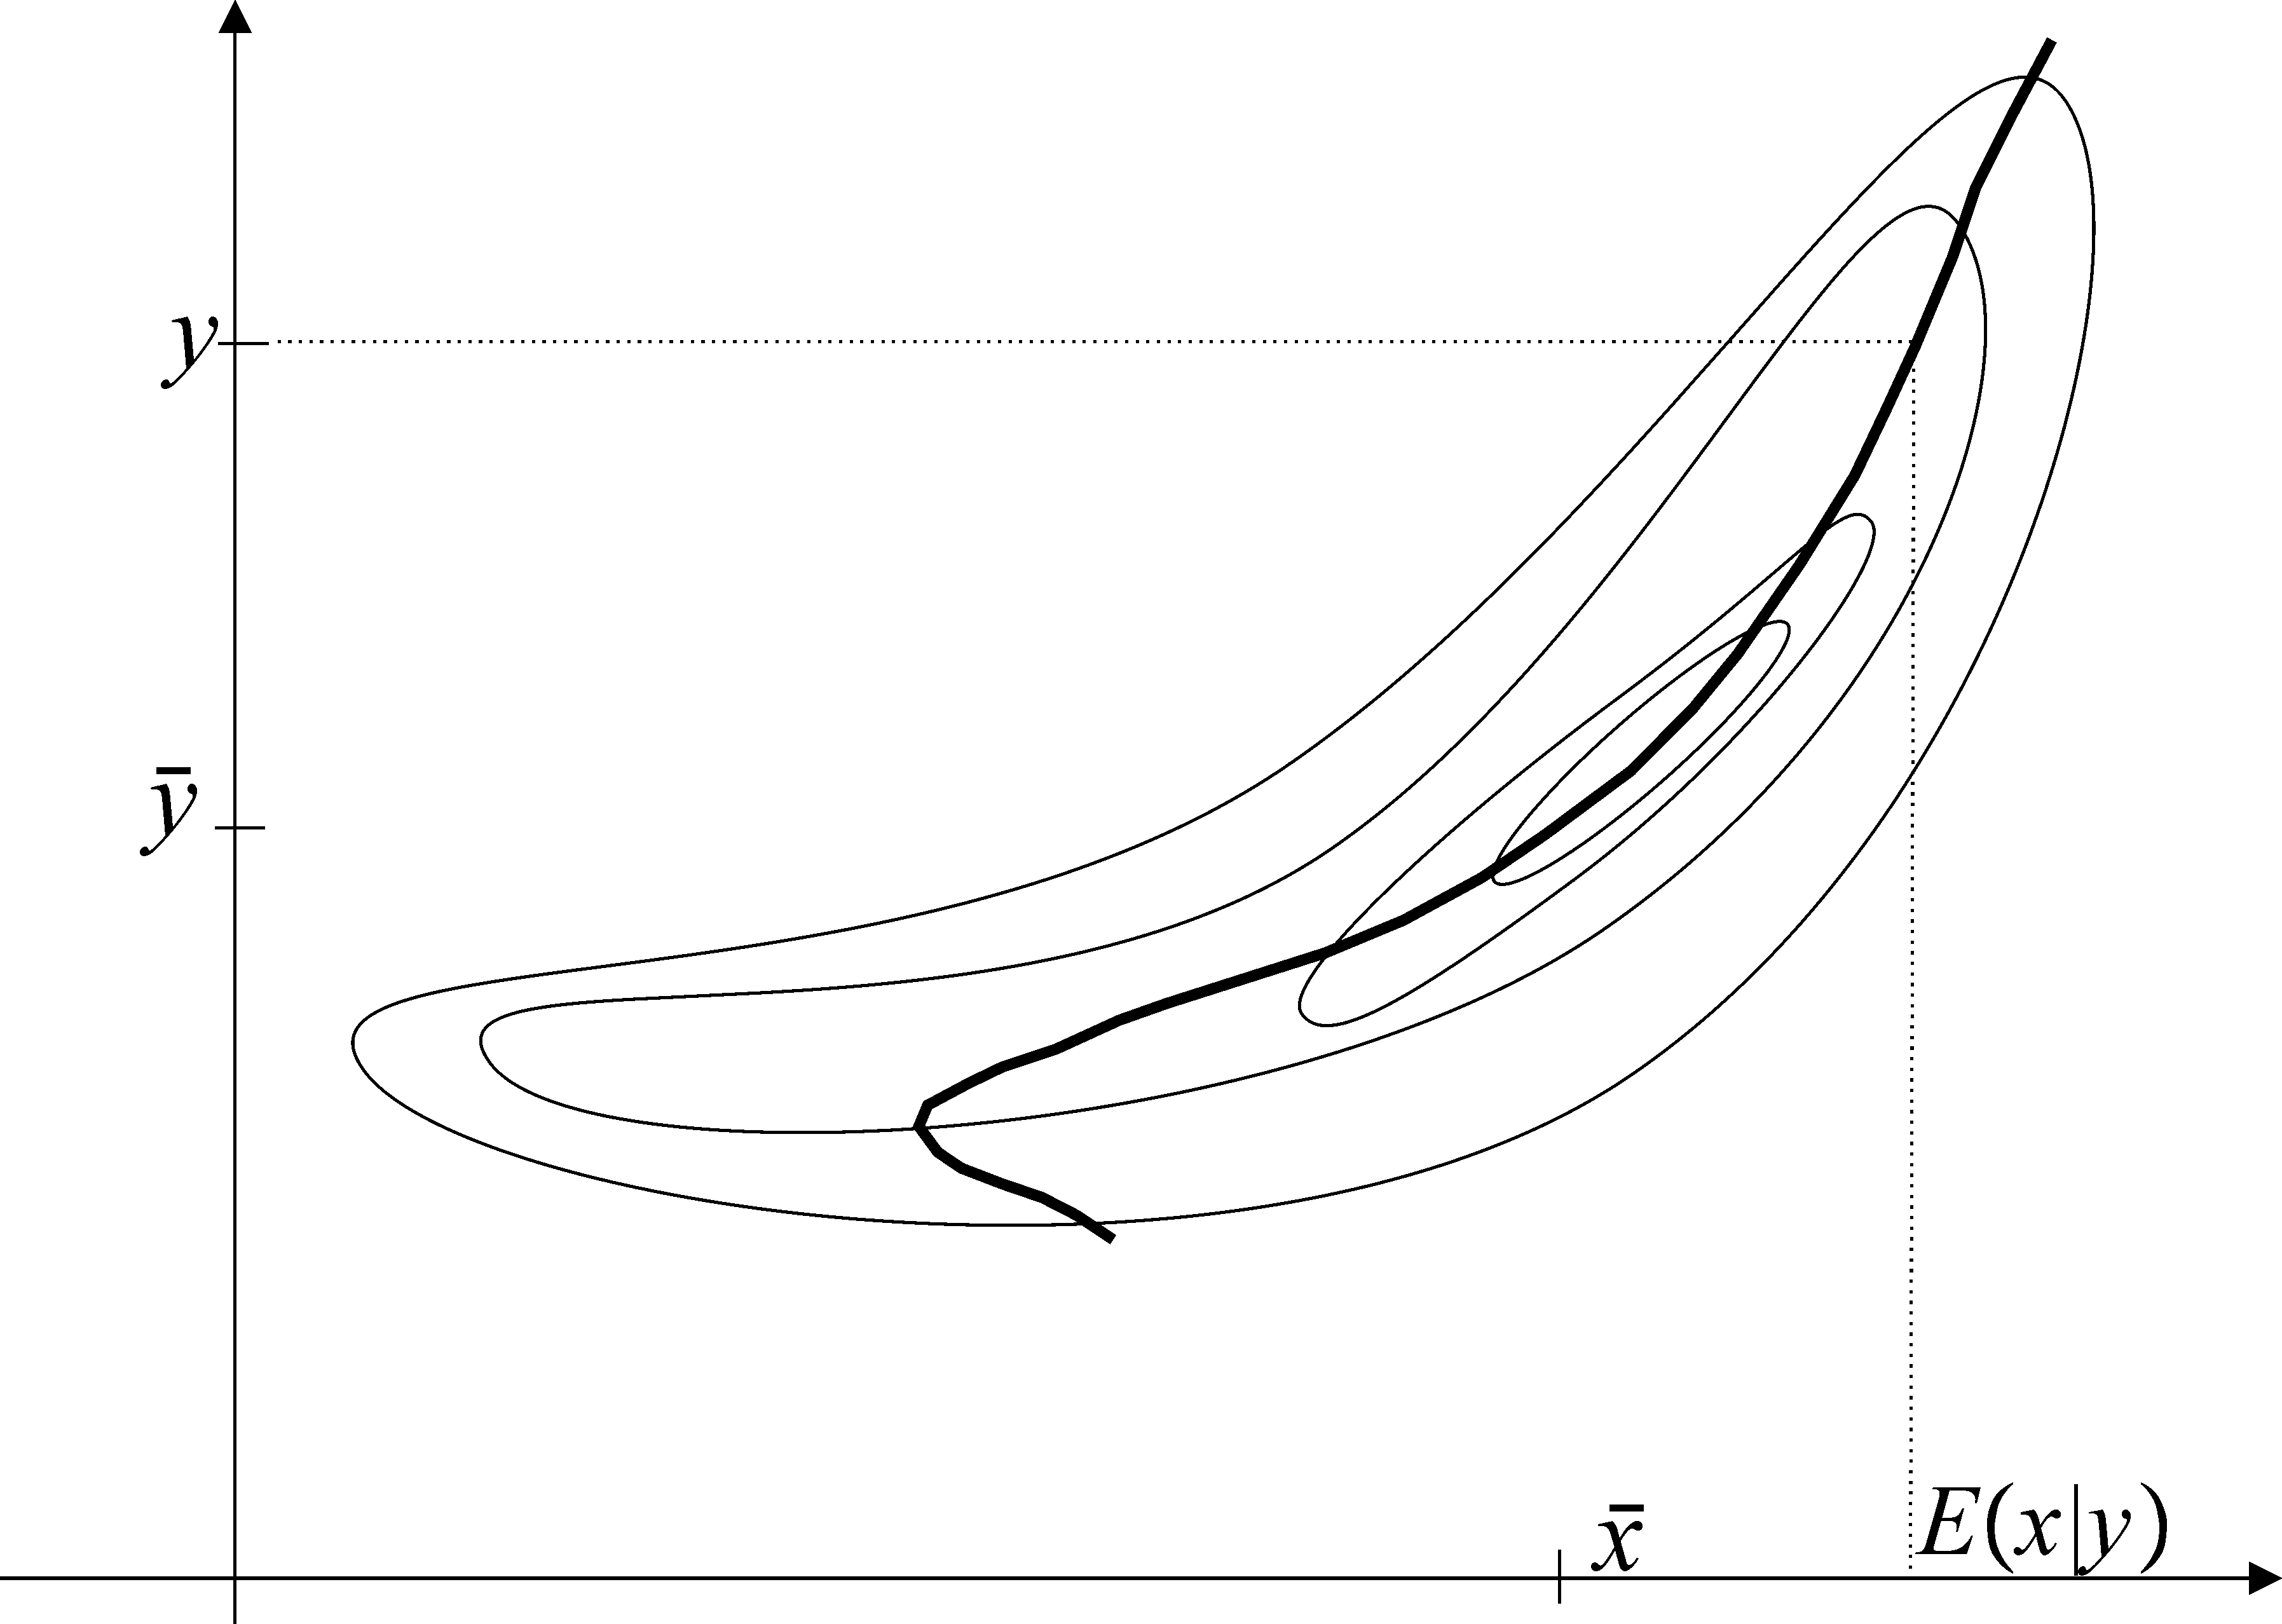
\includegraphics[width=10cm]{best_estimator_gaussian}\caption{Nonlinear estimator $E(x|y)$}

\label{fig:best_estimator_gaussian}
\end{figure}

However, obtaining an analytic expression for such an estimator is
generally not a simple task and it is preferable to limit ourselves
to linear estimators. A \emph{linear estimator} is a linear function
of $\mathbb{R}^{m}\rightarrow\mathbb{R}^{n}$ of the form: 
\begin{equation}
\mathbf{\hat{x}}=\mathbf{Ky}+\mathbf{b}\label{eq:Kyplusb}
\end{equation}
where $\mathbf{K}\in\mathbb{R}^{n\times m}$ and $\mathbf{b}\in\mathbb{R}^{n}$.
In this section, we will propose a method capable of finding a \emph{good}
$\mathbf{K}$ and a \emph{good} $\mathbf{b}$ from the sole knowledge
of the first-order moments $\mathbf{\bar{x}},\mathbf{\bar{y}}$ and
the second-order moments $\mathbf{\boldsymbol{\Gamma}}_{\mathbf{x}},\mathbf{\boldsymbol{\Gamma}}_{\mathbf{x}},\mathbf{\boldsymbol{\Gamma}}_{\mathbf{xy}}$.
The \emph{estimation error} is: 
\[
\boldsymbol{\varepsilon}=\mathbf{\hat{x}}-\mathbf{x}
\]
\begin{figure}[H]
\centering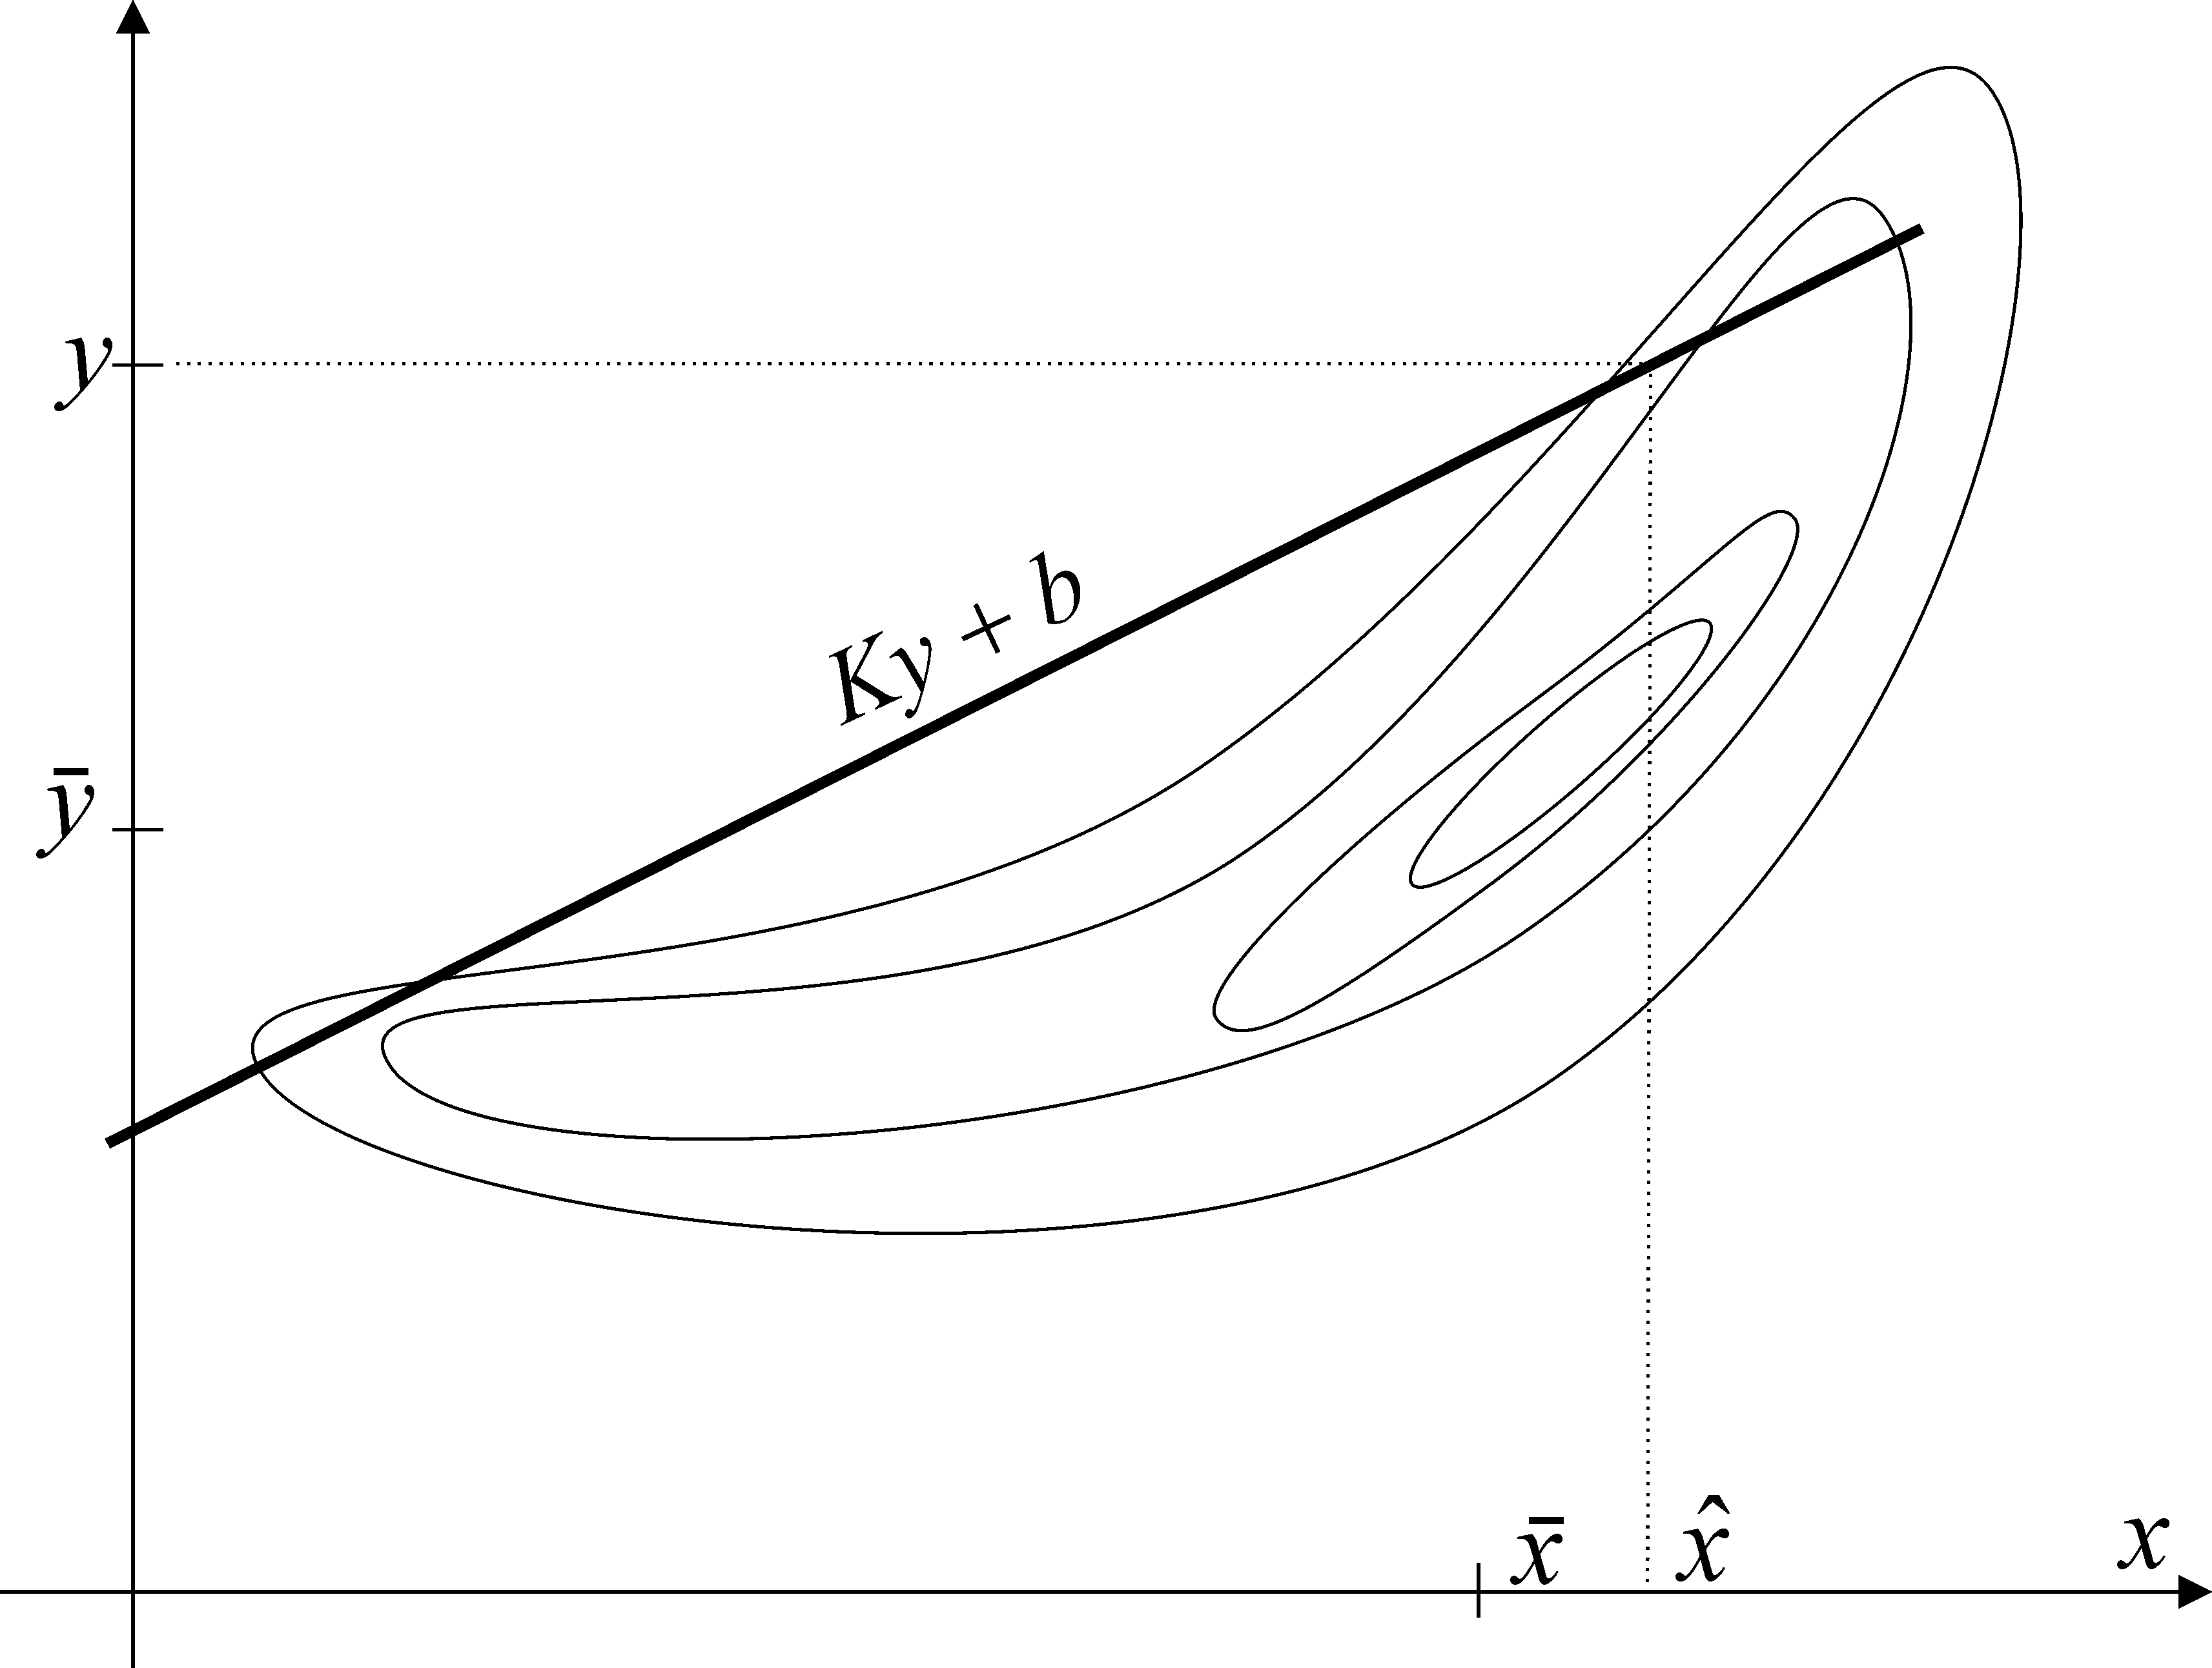
\includegraphics[width=10cm]{best_estimator1}\caption{Biased linear estimator}

\label{fig:best:estimator:1}
\end{figure}

The estimator is said to be \emph{unbiased} if $E\left(\boldsymbol{\varepsilon}\right)=\mathbf{0}$.
It is \emph{orthogonal }if\emph{\ }$E\left(\boldsymbol{\varepsilon}\widetilde{\mathbf{y}}^{\text{T}}\right)=\mathbf{0}$.
This naming comes from the fact that the space of random variables
of $\mathbb{R}$ can be equipped with a scalar product defined by
$\left\langle a,b\right\rangle =E\left(\left(a-\bar{a}\right)\left(b-\bar{b}\right)\right)$
and that if this scalar product is zero, the two random variables
$a$ and $b$ are called orthogonal. In the vector case (which is
that of our paragraph since $\boldsymbol{\varepsilon}$ and $\widetilde{\mathbf{y}}$
are vectors), we say that the two random vectors $\mathbf{a}$ and
$\mathbf{b}$ are orthogonal if their components are, \emph{i.e.,}
$E\left(\left(a_{i}-\bar{a}_{i}\right)\left(b_{j}-\bar{b}_{j}\right)\right)=0$
for all $\left(i,j\right)$, or equivalently $E\left(\left(\mathbf{a}-\mathbf{\bar{a}}\right)\left(\mathbf{b}-\mathbf{\bar{b}}\right)^{\text{T}}\right)=\mathbf{0}$.
Figure \ref{fig:best:estimator:1} represents the contour lines of
a probability law for the pair $\left(x,y\right)$. The line illustrates
a linear estimator. Let us randomly pick a pair $\left(x,y\right)$
while respecting its probability law. It is clear that the probability
to be above the line is high, \emph{i.e.,} the probability to have
$\hat{x}<x$ is high, or even that $E\left(\varepsilon\right)<0$.
The estimator is thus biased. Figure \ref{fig:best_estimator2} represents
four different linear estimators. For estimator (a), $E(\varepsilon)<0$
and for estimator (c), $E(\varepsilon)>0$. For estimators (b) and
(d), $E(\varepsilon)=0$ and therefore the two estimators are unbiased.
However, it is evident that estimator (b) is better. What differentiates
these two is orthogonality. For (d), we have $E\left(\varepsilon\widetilde{y}\right)<0$
(if $\widetilde{y}>0$, $\varepsilon$ tends to be negative whereas
if $\widetilde{y}<0$, $\varepsilon$ tends to be positive).

\begin{figure}[th]
\centering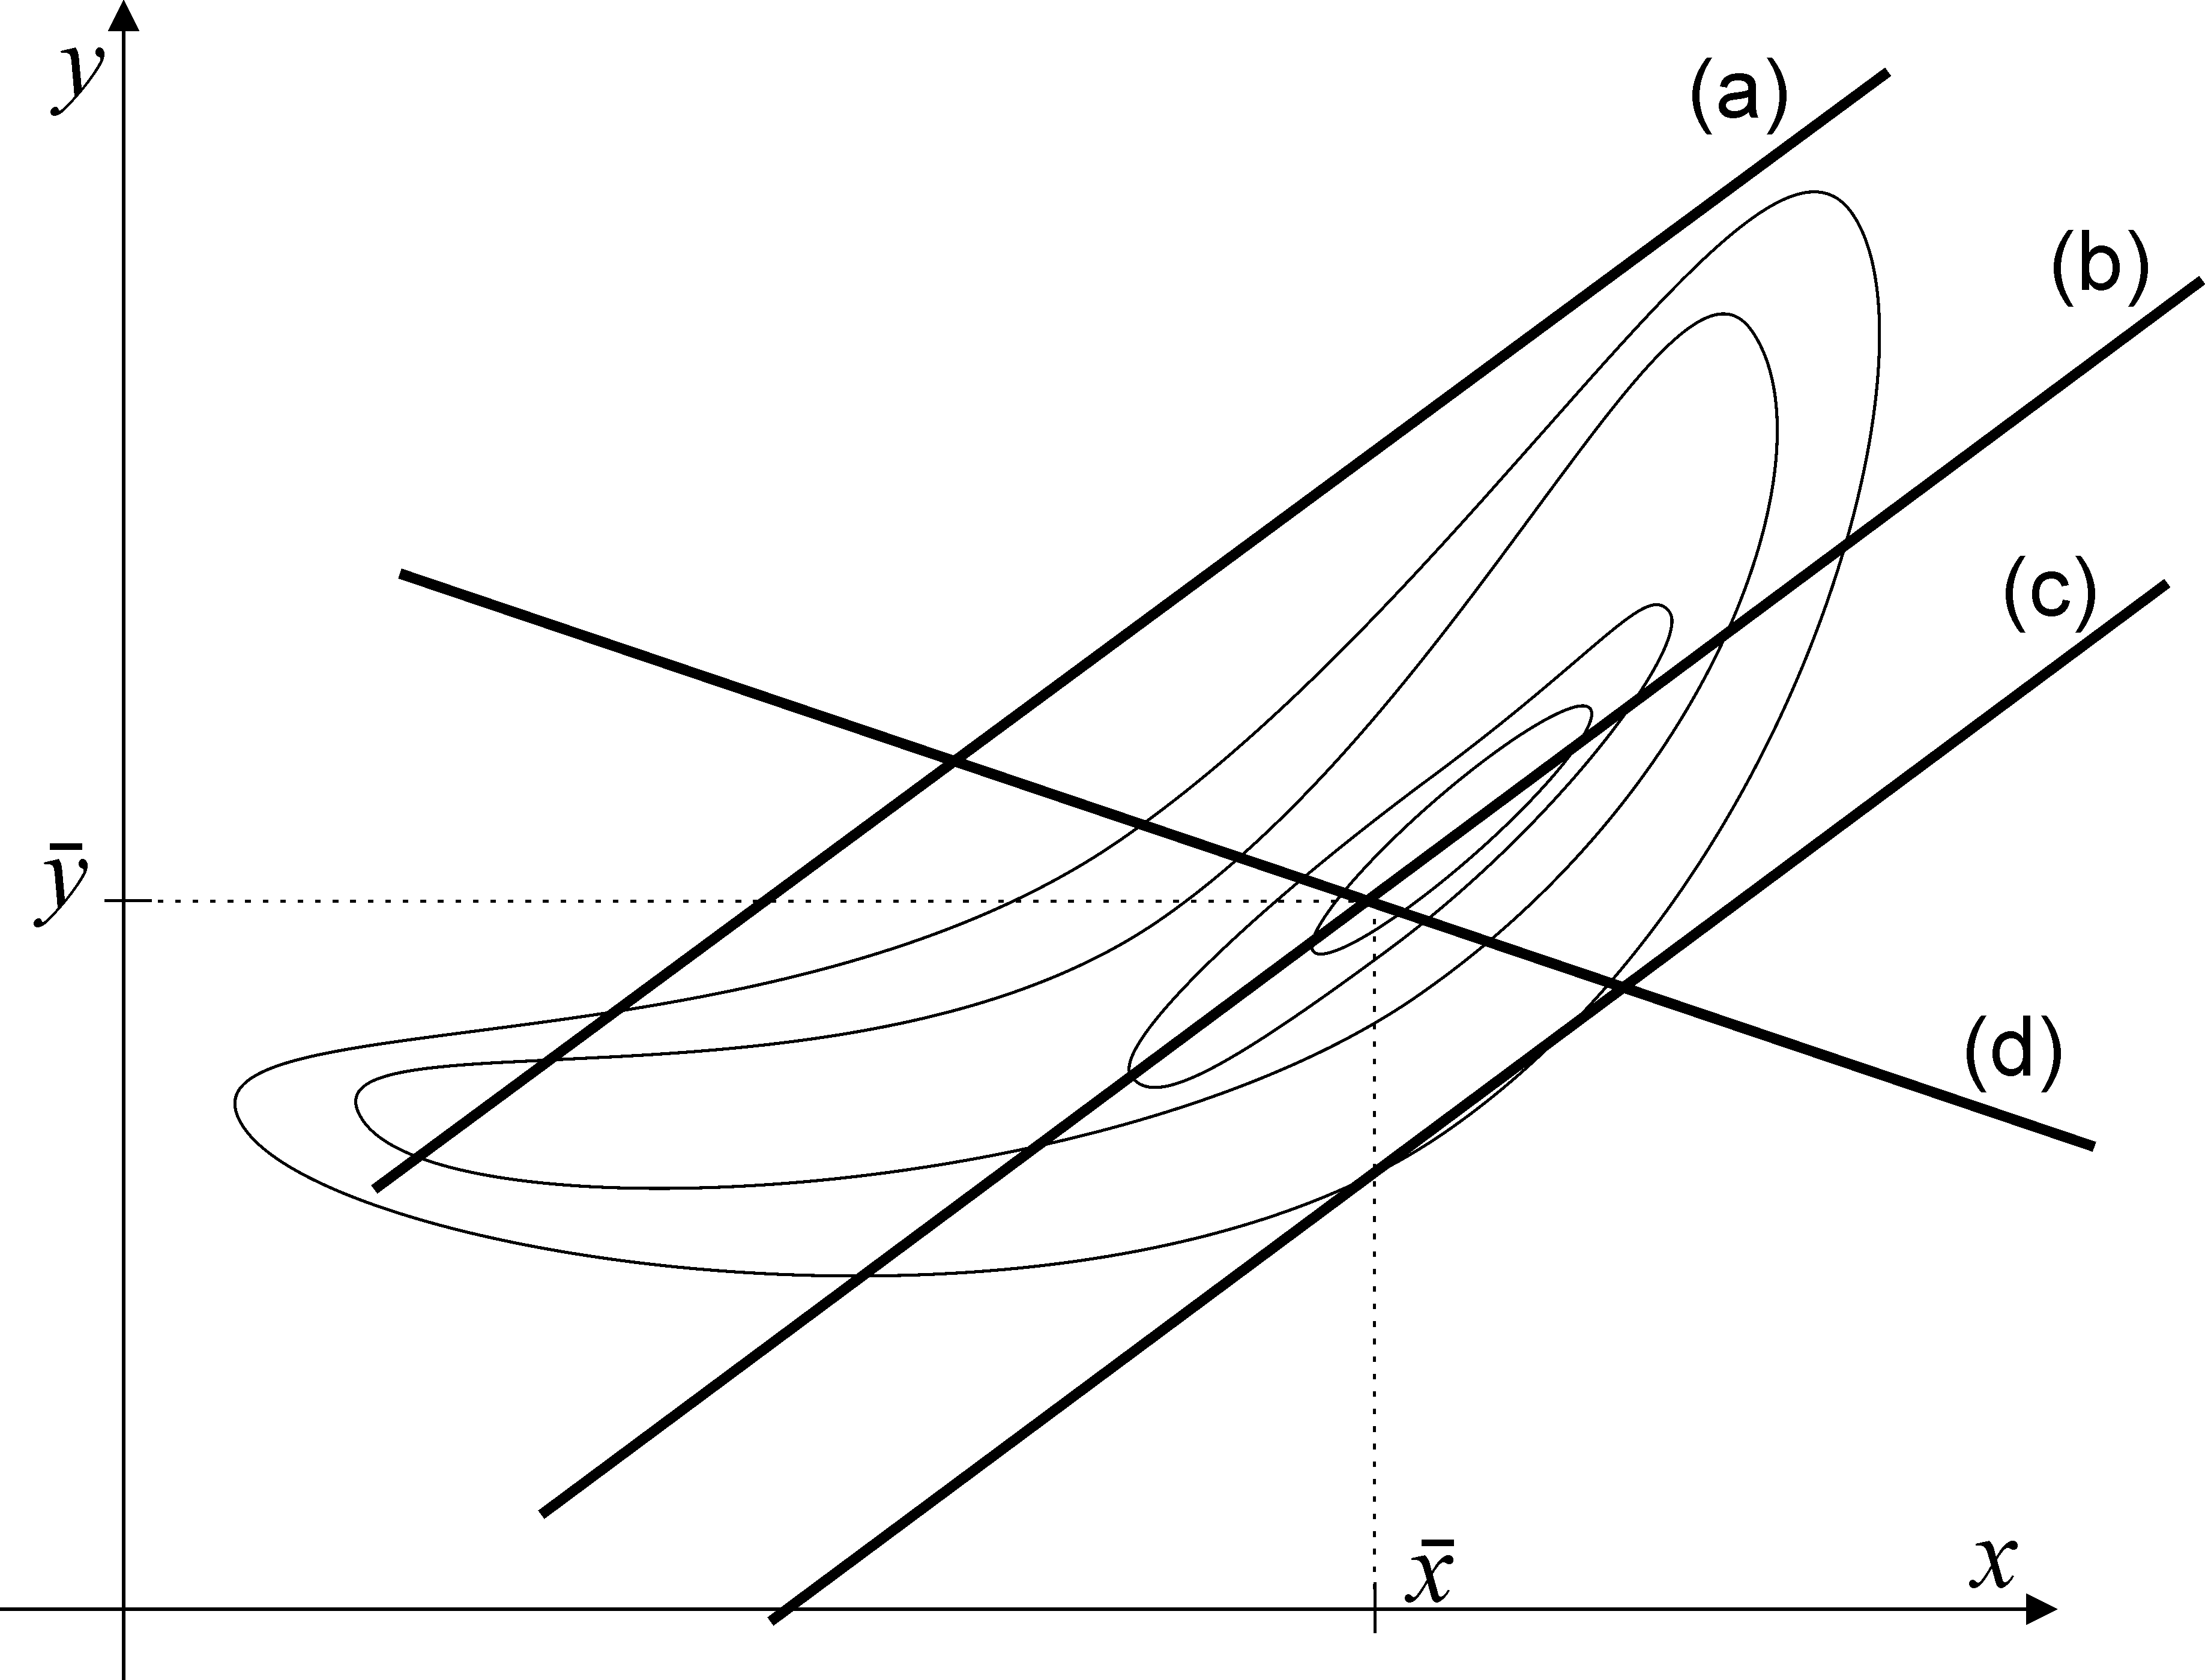
\includegraphics[width=10cm]{best_estimator2}\caption{Among these four linear estimators, estimator (b), which is unbiased
and orthogonal, seems to be the best}

\label{fig:best_estimator2}
\end{figure}

\begin{thm}
Consider two random vectors $\mathbf{x}$ and $\mathbf{y}$. A unique
unbiased orthogonal estimator exists. It is given by: 
\begin{equation}
\mathbf{\hat{x}}=\mathbf{\bar{x}+K}\cdot\left(\mathbf{y}-\mathbf{\bar{y}}\right)\label{eq:ortho:estimator}
\end{equation}
where: 
\begin{equation}
\mathbf{K}=\mathbf{\boldsymbol{\Gamma}}_{\mathbf{xy}}\mathbf{\boldsymbol{\Gamma}}_{\mathbf{y}}^{-1}\label{eq:kalman:gain}
\end{equation}
is referred to as the \emph{Kalman gain}. 
\end{thm}
\textbf{Example}. Let us consider once again the example in Section
\ref{sst:kalman:cov:interpret}. We obtain: 
\[
\hat{x}=\bar{x}+\boldsymbol{\Gamma}_{xy}\boldsymbol{\Gamma}_{y}^{-1}\cdot\left(y-\bar{y}\right)=2+0.1\cdot\left(y-10\right).
\]
The corresponding estimator is illustrated on Figure \ref{fig:kalman_unbiased_ortho}.

\begin{figure}[H]
\centering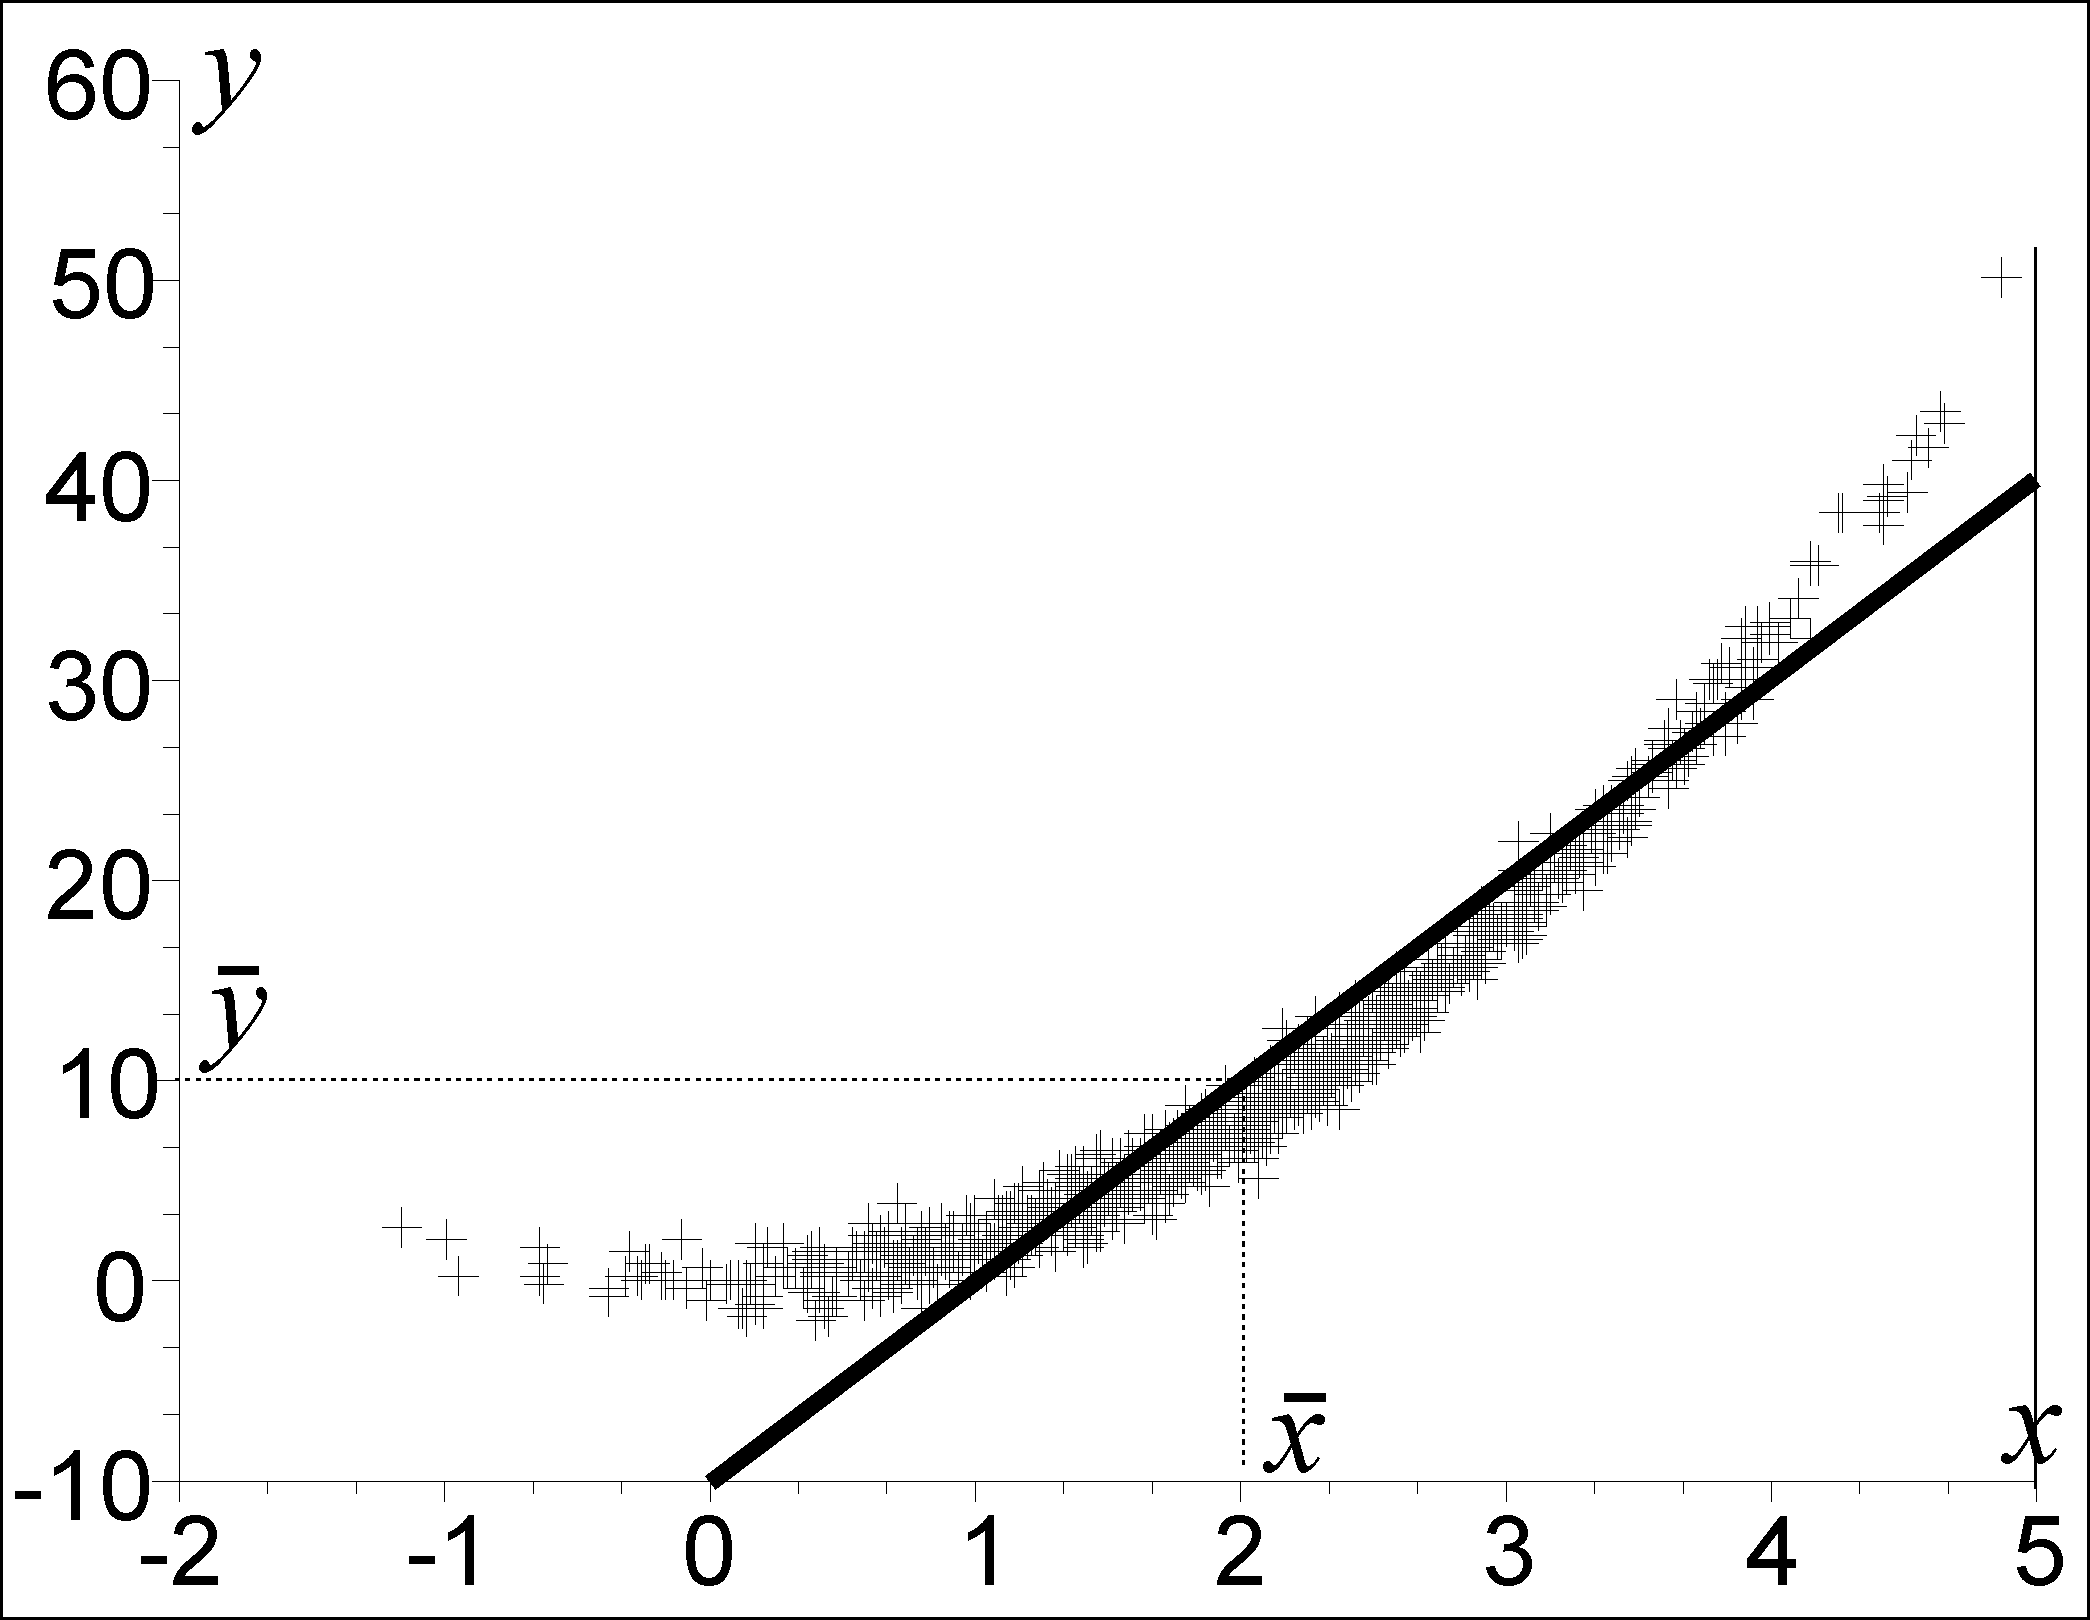
\includegraphics[width=8cm]{kalman_unbiased_ortho}\caption{Unbiased orthogonal linear estimator}

\label{fig:kalman_unbiased_ortho}
\end{figure}

\begin{proof}
\noindent We have: 
\[
\begin{array}{ccl}
E\left(\boldsymbol{\varepsilon}\right) & = & E\left(\mathbf{\hat{x}}-\mathbf{x}\right)\\
 & \overset{\text{(\ref{eq:Kyplusb})}}{=} & E\left(\mathbf{Ky}+\mathbf{b}-\mathbf{x}\right)\\
 & = & \mathbf{K}E\left(\mathbf{y}\right)+\mathbf{b}-E\left(\mathbf{x}\right)\\
 & = & \mathbf{K\bar{y}}+\mathbf{b}-\mathbf{\bar{x}}
\end{array}
\]
The estimator is unbiased if $E\left(\boldsymbol{\varepsilon}\right)=\mathbf{0}$,
\emph{i.e.}: 
\begin{equation}
\mathbf{b}=\mathbf{\bar{x}}-\mathbf{K\bar{y}},\label{eq:biasb}
\end{equation}
which gives us (\ref{eq:ortho:estimator}). In this case: 
\begin{equation}
\boldsymbol{\varepsilon}=\mathbf{\hat{x}}-\mathbf{x}\overset{\text{(\ref{eq:ortho:estimator})}}{=}\mathbf{\bar{x}+K}\cdot\left(\mathbf{y}-\mathbf{\bar{y}}\right)-\mathbf{x}=\mathbf{K}\widetilde{\mathbf{y}}-\widetilde{\mathbf{x}}.\label{eq:eps:unbiased}
\end{equation}
The estimator is orthogonal if: 
\[
\begin{array}{lll}
E\left(\boldsymbol{\varepsilon}\cdot\widetilde{\mathbf{y}}^{\text{T}}\right)=\mathbf{0} & \overset{\text{(\ref{eq:eps:unbiased})}}{\Leftrightarrow} & E\left(\left(\mathbf{K}\widetilde{\mathbf{y}}-\widetilde{\mathbf{x}}\right)\cdot\widetilde{\mathbf{y}}^{\text{T}}\right)=\mathbf{0}\\
 & \Leftrightarrow & E\left(\mathbf{K}\widetilde{\mathbf{y}}\widetilde{\mathbf{y}}^{\text{T}}-\widetilde{\mathbf{x}}\widetilde{\mathbf{y}}^{\text{T}}\right)=\mathbf{0}\\
 & \Leftrightarrow & \mathbf{K\boldsymbol{\Gamma}}_{\mathbf{y}}-\mathbf{\boldsymbol{\Gamma}}_{\mathbf{xy}}=\mathbf{0}\\
 & \Leftrightarrow & \mathbf{K}=\mathbf{\boldsymbol{\Gamma}}_{\mathbf{xy}}\cdot\mathbf{\boldsymbol{\Gamma}}_{\mathbf{y}}^{-1}
\end{array}
\]
which concludes the proof.
\end{proof}
\begin{thm}
The covariance matrix of the error associated with the unbiased orthogonal
linear estimator is: 
\begin{equation}
\mathbf{\boldsymbol{\Gamma}}_{\boldsymbol{\varepsilon}}=\mathbf{\boldsymbol{\Gamma}}_{\mathbf{x}}-\mathbf{K}\cdot\mathbf{\boldsymbol{\Gamma}}_{\mathbf{yx}}.\label{eq:cov_error}
\end{equation}
\end{thm}
\begin{proof}
\noindent The covariance matrix of $\boldsymbol{\varepsilon}$ in
the unbiased case is written as: 
\begin{align*}
\mathbf{\boldsymbol{\Gamma}}_{\boldsymbol{\varepsilon}} & =E\left(\boldsymbol{\varepsilon}\cdot\boldsymbol{\varepsilon}^{\text{T}}\right)\overset{\text{(\ref{eq:eps:unbiased})}}{=}E\left(\left(\mathbf{K}\widetilde{\mathbf{y}}-\widetilde{\mathbf{x}}\right)\cdot\left(\mathbf{K}\widetilde{\mathbf{y}}-\widetilde{\mathbf{x}}\right)^{\text{T}}\right)\\
 & =E\left(\left(\mathbf{K}\widetilde{\mathbf{y}}-\widetilde{\mathbf{x}}\right)\cdot\left(\widetilde{\mathbf{y}}^{\text{T}}\mathbf{K}^{\text{T}}-\widetilde{\mathbf{x}}^{\text{T}}\right)\right)\\
 & =E\left(\mathbf{K}\widetilde{\mathbf{y}}\widetilde{\mathbf{y}}^{\text{T}}\mathbf{K}^{\text{T}}-\widetilde{\mathbf{x}}\widetilde{\mathbf{y}}^{\text{T}}\mathbf{K}^{\text{T}}-\mathbf{K}\widetilde{\mathbf{y}}\widetilde{\mathbf{x}}^{\text{T}}+\widetilde{\mathbf{x}}\widetilde{\mathbf{x}}^{\text{T}}\right).
\end{align*}
Using the linearity of the expectation operator, we get 
\begin{equation}
\mathbf{\boldsymbol{\Gamma}}_{\boldsymbol{\varepsilon}}=~\underset{\overset{\text{(\ref{eq:kalman:gain})}}{=}\mathbf{0}}{\underbrace{(\mathbf{K\boldsymbol{\Gamma}}_{\mathbf{y}}-\mathbf{\boldsymbol{\Gamma}}_{\mathbf{xy}}})}\mathbf{K}^{\text{T}}-\mathbf{K\boldsymbol{\Gamma}}_{\mathbf{yx}}+\mathbf{\boldsymbol{\Gamma}}_{\mathbf{x}}.\label{eq:gamma:eps}
\end{equation}
\end{proof}

\section{Optimality}

We will now present a theorem that shows that the unbiased orthogonal
linear estimator is the best among all unbiased estimators. In order
to understand this concept of \emph{best}, we need to recall the inequalities
on the covariance matrices, which tells us that $\boldsymbol{\Gamma}_{1}\leq\boldsymbol{\Gamma}_{2}$
if and only if \textbf{$\Delta~$}$=\boldsymbol{\Gamma}_{2}-\boldsymbol{\Gamma}_{1}$
is a covariance matrix.
\begin{thm}
No unbiased linear estimator exists allowing to obtain a smaller covariance
matrix on the error $\mathbf{\boldsymbol{\Gamma}}_{\boldsymbol{\varepsilon}}$
than the one given by the orthogonal estimator.
\end{thm}
\vspace*{-2mm}

\begin{proof}
\noindent Every possible matrix $\mathbf{K}$ for our unbiased linear
estimator is written in the form $\mathbf{K}=\mathbf{K}_{0}+\mathbf{\Delta}$
with $\mathbf{K}_{0}=\mathbf{\boldsymbol{\Gamma}}_{\mathbf{xy}}\mathbf{\boldsymbol{\Gamma}}_{\mathbf{y}}^{-1}$
and $\mathbf{\Delta}$ being an arbitrary matrix. Following (\ref{eq:gamma:eps}),
the covariance matrix for the error is:
\[
\begin{array}{lll}
\mathbf{\boldsymbol{\Gamma}}_{\boldsymbol{\varepsilon}} & = & \left(\left(\mathbf{K}_{0}+\mathbf{\Delta}\right)\mathbf{\boldsymbol{\Gamma}}_{\mathbf{y}}-\mathbf{\boldsymbol{\Gamma}}_{\mathbf{xy}}\right)\left(\mathbf{K}_{0}+\mathbf{\Delta}\right)^{\text{T}}-\left(\mathbf{K}_{0}+\mathbf{\Delta}\right)\mathbf{\boldsymbol{\Gamma}}_{\mathbf{yx}}+\mathbf{\boldsymbol{\Gamma}}_{\mathbf{x}}\\
 & = & \left(\mathbf{K}_{0}+\mathbf{\Delta}\right)(\underset{=\mathbf{\boldsymbol{\Gamma}}_{\mathbf{yx}}}{\underbrace{\mathbf{\boldsymbol{\Gamma}}_{\mathbf{y}}\mathbf{K}_{0}^{\text{T}}}}+\mathbf{\boldsymbol{\Gamma}}_{\mathbf{y}}\mathbf{\Delta}^{\text{T}})-(\underset{=\mathbf{K}_{0}\mathbf{\boldsymbol{\Gamma}}_{\mathbf{yx}}}{\underbrace{\mathbf{\boldsymbol{\Gamma}}_{\mathbf{xy}}\mathbf{K}_{0}^{\text{T}}}}+\mathbf{\boldsymbol{\Gamma}}_{\mathbf{xy}}\mathbf{\Delta}^{\text{T}})-\left(\mathbf{K}_{0}\mathbf{\boldsymbol{\Gamma}}_{\mathbf{yx}}+\mathbf{\Delta\boldsymbol{\Gamma}}_{\mathbf{yx}}\right)+\mathbf{\boldsymbol{\Gamma}}_{\mathbf{x}}\\
 & = & \mathbf{K}_{0}\mathbf{\boldsymbol{\Gamma}}_{\mathbf{yx}}+\mathbf{\Delta\boldsymbol{\Gamma}}_{\mathbf{yx}}+\underset{=\mathbf{\boldsymbol{\Gamma}}_{\mathbf{xy}}}{\underbrace{\mathbf{K}_{0}\mathbf{\boldsymbol{\Gamma}}_{\mathbf{y}}}}\mathbf{\Delta}^{\text{T}}+\mathbf{\Delta\boldsymbol{\Gamma}}_{\mathbf{y}}\mathbf{\Delta}^{\text{T}}-\mathbf{K}_{0}\mathbf{\boldsymbol{\Gamma}}_{\mathbf{yx}}-\mathbf{\boldsymbol{\Gamma}}_{\mathbf{xy}}\mathbf{\Delta}^{\text{T}}-\mathbf{K}_{0}\mathbf{\boldsymbol{\Gamma}}_{\mathbf{yx}}-\mathbf{\Delta\boldsymbol{\Gamma}}_{\mathbf{yx}}+\mathbf{\boldsymbol{\Gamma}}_{\mathbf{x}}\\
 & = & -\mathbf{K}_{0}\mathbf{\boldsymbol{\Gamma}}_{\mathbf{yx}}+\mathbf{\Delta\boldsymbol{\Gamma}}_{\mathbf{y}}\mathbf{\Delta}^{\text{T}}+\mathbf{\boldsymbol{\Gamma}}_{\mathbf{x}}.
\end{array}
\]
\end{proof}
Since $\mathbf{\Delta\boldsymbol{\Gamma}}_{\mathbf{y}}\mathbf{\Delta}^{\text{T}}$
is always positive symmetric, the covariance matrix $\mathbf{\boldsymbol{\Gamma}}_{\boldsymbol{\varepsilon}}$
is minimal for $\mathbf{\Delta}=\mathbf{0}$, i.e. for $\mathbf{K}=\mathbf{\boldsymbol{\Gamma}}_{\mathbf{xy}}\mathbf{\boldsymbol{\Gamma}}_{\mathbf{y}}^{-1}$,
which corresponds to the orthogonal unbiased estimator.

\section{Application to linear estimation}

Let us assume that $\mathbf{x}$ and $\mathbf{y}$ are related by
the relation 
\[
\mathbf{y}=\mathbf{Cx}+\mathbf{\boldsymbol{\beta}}
\]
where $\mathbf{\boldsymbol{\beta}}$ is a centered random vector non-correlated
with $\mathbf{x}$. The covariance matrices of $\mathbf{x}$ and $\mathbf{\boldsymbol{\beta}}$
are denoted by $\mathbf{\boldsymbol{\Gamma}}_{\mathbf{x}}$ and $\mathbf{\boldsymbol{\Gamma}}_{\mathbf{\boldsymbol{\beta}}}$.
Let us use the results obtained in the previous section in order to
find the best unbiased linear estimator for $\mathbf{x}$ (refer to
\cite{Walter14} for more details on linear estimation). 

We have:
\begin{equation}
\begin{array}{lcl}
\mathbf{\bar{y}} & = & \mathbf{C\bar{x}}+\mathbf{\bar{\boldsymbol{\beta}}}=\mathbf{C\bar{x}}\\
\mathbf{\boldsymbol{\Gamma}}_{\mathbf{y}} & \overset{\text{(\ref{eq:matcov:linear})}}{=} & \mathbf{C\boldsymbol{\Gamma}}_{\mathbf{x}}\mathbf{C}^{\text{T}}+\mathbf{\boldsymbol{\Gamma}}_{\mathbf{\boldsymbol{\beta}}}\\
\mathbf{\boldsymbol{\Gamma}}_{\mathbf{xy}} & = & E\left(\widetilde{\mathbf{x}}\cdot\widetilde{\mathbf{y}}^{\text{T}}\right)=E\left(\widetilde{\mathbf{x}}\cdot\left(\mathbf{C}\widetilde{\mathbf{x}}+\widetilde{\mathbf{\boldsymbol{\beta}}}\right)^{\text{T}}\right)=E\left(\widetilde{\mathbf{x}}\cdot\widetilde{\mathbf{x}}^{\text{T}}\mathbf{C}^{\text{T}}+\widetilde{\mathbf{x}}\cdot\widetilde{\mathbf{\boldsymbol{\beta}}}^{\text{T}}\right)\\
 & = & E\left(\widetilde{\mathbf{x}}\cdot\widetilde{\mathbf{x}}^{\text{T}}\right)\mathbf{C}^{\text{T}}+~\underset{=\ \mathbf{0}}{\underbrace{E\left(\widetilde{\mathbf{x}}\cdot\widetilde{\mathbf{\boldsymbol{\beta}}}^{\text{T}}\right)}}\ =\mathbf{\boldsymbol{\Gamma}}_{\mathbf{x}}\mathbf{C}^{\text{T}}.
\end{array}\label{eq:lin_estim:0}
\end{equation}
Consequently, the best unbiased estimator for $\mathbf{x}$ and covariance
matrix of the error can be obtained from $\mathbf{\mathbf{\boldsymbol{\Gamma}}_{\mathbf{x}}},\mathbf{\boldsymbol{\Gamma}}_{\mathbf{\boldsymbol{\beta}}},\mathbf{C},\mathbf{\bar{x}}$
by using the following formulas:
\begin{equation}
\begin{array}{lllll}
\text{(i)} & \mathbf{\hat{x}} & \overset{\text{(\ref{eq:ortho:estimator})}}{=} & \mathbf{\bar{x}+K}\widetilde{\mathbf{y}} & \text{(estimation)}\\
\text{(ii)} & \mathbf{\boldsymbol{\Gamma}}_{\mathbf{\varepsilon}} & \overset{\text{(\ref{eq:cov_error})}}{=} & \mathbf{\boldsymbol{\Gamma}}_{\mathbf{x}}-\mathbf{KC\boldsymbol{\Gamma}}_{\mathbf{x}} & \text{(covariance of the error)}\\
\text{(iii)} & \widetilde{\mathbf{y}} & \overset{\text{(\ref{eq:lin_estim:0})}}{=} & \mathbf{y}-\mathbf{C\bar{x}} & \text{(innovation)}\\
\text{(iv)} & \mathbf{\boldsymbol{\Gamma}}_{\mathbf{y}} & \overset{\text{(\ref{eq:lin_estim:0})}}{=} & \mathbf{C\boldsymbol{\Gamma}}_{\mathbf{x}}\mathbf{C}^{\text{T}}+\mathbf{\boldsymbol{\Gamma}}_{\mathbf{\boldsymbol{\beta}}} & \text{(covariance of the innovation)}\\
\text{(v)} & \mathbf{K} & \overset{\text{(\ref{eq:kalman:gain},\ref{eq:lin_estim:0})}}{=} & \mathbf{\mathbf{\boldsymbol{\Gamma}}_{\mathbf{x}}\mathbf{C}}^{\text{T}}\mathbf{\boldsymbol{\Gamma}}_{\mathbf{y}}^{-1} & \text{(Kalman gain)}
\end{array}\label{eq:linear:estim}
\end{equation}

\textbf{Remark}. Figure \ref{fig:best_estimator_gaussian} illustrates
a situation in which it could be advantageous not to use a linear
estimator. Here, the chosen estimator corresponds to $\hat{x}=$ $E\left(x|y\right)$.
In the particular case where the pair $\left(\mathbf{x},\mathbf{y}\right)$
is Gaussian, the estimator $\mathbf{\hat{x}}=E\left(\mathbf{x}|\mathbf{y}\right)$
corresponds to the unbiased orthogonal estimator. In this case, we
have, following (\ref{eq:linear:estim}):
\[
\begin{array}{lll}
E\left(\mathbf{x}|\mathbf{y}\right) & = & \mathbf{\bar{x}+\boldsymbol{\Gamma}}_{\mathbf{xy}}\mathbf{\boldsymbol{\Gamma}}_{\mathbf{y}}^{-1}\left(\mathbf{y}-\mathbf{\bar{y}}\right)\\
E\left(\mathbf{\varepsilon}\cdot\mathbf{\varepsilon}^{\text{T}}|\mathbf{y}\right) & = & E\left(\left(\mathbf{\hat{x}}-\mathbf{x}\right)\left(\mathbf{\hat{x}}-\mathbf{x}\right)^{\text{T}}|\mathbf{y}\right)\\
 & = & \mathbf{\boldsymbol{\Gamma}}_{\mathbf{x}}-\mathbf{K}\mathbf{C\boldsymbol{\Gamma}}_{\mathbf{x}}\\
 & = & \mathbf{\boldsymbol{\Gamma}}_{\mathbf{x}}-\mathbf{\boldsymbol{\Gamma}}_{\mathbf{xy}}\mathbf{\boldsymbol{\Gamma}}_{\mathbf{y}}^{-1}\mathbf{\boldsymbol{\Gamma}}_{\mathbf{yx}}
\end{array}
\]


\chapter*{Exercises}

\rule{0.95\columnwidth}{1pt}

\begin{Exercice} \label{ex:ellipsoide:confiance:estimateur} Confidence
ellipse: correction \end{Exercice}

\textcolor{blue}{See the correction video at \href{https://youtu.be/Rmx7nIEwpBg}{https://youtu.be/Rmx7nIEwpBg}}

1) Generate a Gaussian point cloud of $n=1~000$ points associated
with the random vector $\mathbf{x}$ with: 
\[
\mathbf{\bar{x}}=\left(\begin{array}{c}
1\\
2
\end{array}\right)\text{ and }\boldsymbol{\Gamma}_{\mathbf{x}}=\left(\begin{array}{ccc}
3 & \, & 1\\
1 &  & 3
\end{array}\right).
\]
Use a two-line, $n$-column matrix to store the clouds.

2) Find an unbiased and orthogonal linear estimator which allows to
find $x_{1}$ from $x_{2}$. Draw this estimator.

3) Same question as above, but one that allows to find $x_{2}$ from
$x_{1}$. Draw the estimator and discuss the difference with the previous
question.

\rule{0.95\columnwidth}{1pt}

\begin{Exercice} \label{ex:matrice:cov} Covariance matrix propagation
\end{Exercice}

\textcolor{blue}{See the correction video at \href{https://youtu.be/e0iRudPE8-Y}{https://youtu.be/e0iRudPE8-Y}}

Consider three centered random vectors $\mathbf{a},\mathbf{b},\mathbf{c}$
with covariance matrices equal to the identity matrix. These three
vectors are independent of each other. Let $\mathbf{x},\mathbf{y}$
be two random vectors defined as follows: 
\[
\begin{array}{lll}
\mathbf{x} & = & \mathbf{A\cdot a}-\mathbf{b}\\
\mathbf{y} & = & \mathbf{C}\cdot\mathbf{x}+\mathbf{c}
\end{array}
\]
where $\mathbf{A},\mathbf{C}$ are matrices that are known.

1) Give the expression of the mathematical expectations $\mathbf{\bar{x}},\mathbf{\bar{y}}$
and of the covariance matrices $\mathbf{\boldsymbol{\Gamma}}_{\mathbf{x}},\mathbf{\boldsymbol{\Gamma}}_{\mathbf{y}}$
of these two vectors, in function of $\mathbf{A}$ and $\mathbf{C}$.

2) We form the vector $\mathbf{v}=(\mathbf{x~},~\mathbf{y})$. Calculate
the mathematical expectation $\mathbf{\bar{v}}$ and the covariance
matrix $\boldsymbol{\Gamma}_{\mathbf{v}}$ for $\mathbf{v}$.

3) Deduce from the previous question the covariance matrix of the
random vector $\mathbf{z}=\mathbf{y}-\mathbf{x}$. We assume that
$\mathbf{x}$ and $\mathbf{y}$ have same dimension.

4) We measure $\mathbf{y}$, which means that now the random vector
$\mathbf{y}$ becomes deterministic and is well-known. Give an estimation
$\mathbf{\hat{x}}$ for $\mathbf{x}$ using an unbiased and orthogonal
linear estimator.

\rule{0.95\columnwidth}{1pt}

\begin{Exercice} \label{ex:trois:equations} Solving three equations
using a linear estimator$~$ \end{Exercice}

\textcolor{blue}{See the correction video at \href{https://youtu.be/Rst52D2GXM0}{https://youtu.be/Rst52D2GXM0}}

The linear estimator can be used to solve problems that can be translated
as linear equations. Let us consider as an illustration the system:
\[
\left\{ \begin{array}{lll}
2x_{1}+3x_{2} & = & 8\\
3x_{1}+2x_{2} & = & 7\\
x_{1}-x_{2} & = & 0
\end{array}\right.
\]
Since we have more equations than unknowns, the linear estimator must
find some sort of compromise between all of these equations. Let us
assume that the errors $\varepsilon_{i}$ over the $i^{th}$ equation
are centered and with variances : $\sigma_{1}^{2}=1,$ $\sigma_{2}^{2}=4$
and $\sigma_{3}^{2}=4$. Solve the system by using a linear estimator
and find the associated covariance matrix.

\rule{0.95\columnwidth}{1pt}

\begin{Exercice} \label{ex:regression:moteurcc} Estimating the parameters
of an electric motor using a linear estimator$~$ \end{Exercice}

\textcolor{blue}{See the correction video at \href{https://youtu.be/vCCbSvANT7M}{https://youtu.be/vCCbSvANT7M}}

Let us consider a DC motor whose parameters have been estimated with
a least squares method (see Exercise \ref{ex:mc:moteurcc}). Recall
that in that example, the angular speed $\Omega$ of a DC motor verifies
the relation: 
\[
\Omega=x_{1}U+x_{2}T_{r}
\]
where $U$ is the input voltage, $T_{r}$ is the resistive torque
and $\mathbf{x}=\left(x_{1},x_{2}\right)$ is the vector of parameters
that we need to estimate. The following table recalls the measurements
made on the motor for various experimental conditions:
\[
\begin{tabular}{|c|c|c|c|c|c|}
\hline  \ensuremath{U(\text{V})}  &  \ensuremath{4}  &  \ensuremath{10}  &  \ensuremath{10}  &  \ensuremath{13}  &  \ensuremath{15}\\
\hline  \ensuremath{T_{r}(\text{Nm})}  &  \ensuremath{0}  &  \ensuremath{1}  &  \ensuremath{5}  &  \ensuremath{5}  &  \ensuremath{3}\\
\hline  \ensuremath{\Omega(}rad\ensuremath{/\sec)}  &  \ensuremath{5}  &  \ensuremath{10}  &  \ensuremath{8}  &  \ensuremath{14}  &  \ensuremath{17} 
\\\hline \end{tabular}
\]
We assume that the variance of the measurement error is equal to $9$
and does not depend on the experimental conditions. Moreover, we assume
that we know \emph{a priori} that $x_{1}\simeq1$ and $x_{2}\simeq-1$
with a variance of $4$. Estimate the parameters of the motor and
find the associated covariance matrix.

\rule{0.95\columnwidth}{1pt}

\begin{Exercice} \label{ex:kalman:mobile} Trochoid \end{Exercice}

\textcolor{blue}{See the correction video at \href{https://youtu.be/tzkliJQQj7g}{https://youtu.be/tzkliJQQj7g}}

A point mass (placed on a wheel) is moving following a trochoid of
the form: 
\[
\left\{ \begin{array}{lll}
x\left(t\right) & = & p_{1}t-p_{2}\sin t\\
y\left(t\right) & = & p_{1}-p_{2}\cos t
\end{array}\right.
\]
where $x$ corresponds to the abscissa and $y$ to the altitude of
the mass. We measure $y$ for various instants $t$:
\[
\begin{tabular}{|c|cccc|}
\hline  \ensuremath{t}(sec)  &  \ensuremath{1}  &  \ensuremath{2}  &  \ensuremath{3}  &  \ensuremath{7}\\
\hline  \ensuremath{y}(m)  &  \ensuremath{0.38}  &  \ensuremath{3.25}  &  \ensuremath{4.97}  &  \ensuremath{-0.26} 
\\\hline \end{tabular}
\]
The measurement errors have a standard deviation of $10~$cm. 

1) Using an unbiased orthogonal filter, compute an estimation for
$p_{1}$ and $p_{2}$.

2) Draw the estimated path of the mass.


\chapter{Kalman filter\label{ch:filtre:de:Kalman}}

When we control a system, such as a robot, we generally assume that
the state vector was completely known. However, this is not the case
in practice. This vector must be estimated from sensor measurements.
In the case where the only unknown variables are associated with the
position of the robot, Chapter \ref{ch:localisation} gives guidelines
to find them. In the more general case, \emph{filtering}\index{filtering}
or \emph{state observation} seeks to reconstruct this state vector
as well as possible from all the data measured on the robot throughout
time by taking into account the state equations. The aim of this chapter
is to show how such reconstruction is performed, within a stochastic
context in which the system to observe is assumed to be linear. This
is the purpose of the Kalman filter \cite{Kalman60} which will be
developed in this chapter. The Kalman filter is used in numerous mobile
robotics applications, even though the robots in question are strongly
nonlinear. For such applications, the initial conditions are assumed
to be relatively well known in order to allow a reliable linearization.

\section{Equations of the Kalman filter\label{sec:Kalman-filter}}

This paragraph presents the Kalman filter (refer to \cite{DeLarminat93}
for more information). Let us consider the system described by the
following state equations: 
\[
\left\{ \begin{array}{ccl}
\mathbf{x}_{k+1} & = & \mathbf{A}_{k}\mathbf{x}_{k}+\mathbf{u}_{k}+\mathbf{\boldsymbol{\alpha}}_{k}\\
\mathbf{y}_{k} & = & \mathbf{C}_{k}\mathbf{x}_{k}+\mathbf{\boldsymbol{\beta}}_{k}
\end{array}\right.
\]
where $\boldsymbol{\alpha}_{k}$ and $\boldsymbol{\beta}_{k}$ are
random, independent Gaussian noises white in time. By white in time
we mean that the vectors $\boldsymbol{\alpha}_{k_{1}}$ and $\boldsymbol{\alpha}_{k_{2}}$
(or $\boldsymbol{\beta}_{k_{1}}$ and $\boldsymbol{\beta}_{k_{2}}$)
are independent of one another if $k_{1}\neq k_{2}$. The Kalman filter
alternates between two phases: \emph{correction} and \emph{\ prediction}.
To understand the mechanism of the filter, let us position ourselves
at time $k$ and assume that we have already processed the measurements
$\mathbf{y}_{0},\mathbf{y}_{1},\dots,\mathbf{y}_{k-1}$. At this stage,
the state vector is a random vector that we will denote by $\mathbf{x}_{k|k-1}$
(since we are at time $k$ and the measurements have been processed
until $k-1$). This random vector is represented by an estimation
denoted by $\mathbf{\hat{x}}_{k|k-1}$ and a covariance matrix $\mathbf{\boldsymbol{\Gamma}}_{k|k-1}$.

\textbf{Correction}\index{correction}. Let us take the measurement
$\mathbf{y}_{k}$. The random vector representing the state is now
$\mathbf{x}_{k|k}$, which is different than $\mathbf{x}_{k|k-1}$
since $\mathbf{x}_{k|k}$ has knowledge of the measurement $\mathbf{y}$.
The expectation $\mathbf{\hat{x}}_{k|k}$ and the covariance matrix
$\mathbf{\boldsymbol{\Gamma}}_{k|k}$ associated to $\mathbf{x}_{k|k}$
are given by Equations (\ref{eq:linear:estim}). We therefore have:
\begin{equation}
\begin{array}{lllll}
\text{(i)} & \mathbf{\hat{x}}_{k|k} & = & \mathbf{\hat{x}}_{k|k-1}+\mathbf{K}_{k}\cdot\widetilde{\mathbf{y}}_{k} & \text{(corrected estimation)}\\
\text{(ii)} & \mathbf{\boldsymbol{\Gamma}}_{k|k} & = & \mathbf{\mathbf{\boldsymbol{\Gamma}}}_{k|k-1}-\mathbf{K}_{k}\cdot\mathbf{C}_{k}\mathbf{\mathbf{\boldsymbol{\Gamma}}}_{k|k-1} & \text{(corrected covariance)}\\
\text{(iii)} & \widetilde{\mathbf{y}}_{k} & = & \mathbf{y}_{k}-\mathbf{C}_{k}\mathbf{\hat{x}}_{k|k-1} & \text{(innovation)}\\
\text{(iv)} & \mathbf{S}_{k} & = & \mathbf{C}_{k}\mathbf{\mathbf{\boldsymbol{\Gamma}}}_{k|k-1}\mathbf{C}_{k}^{\text{T}}+\mathbf{\boldsymbol{\Gamma}}_{\mathbf{\boldsymbol{\beta}}_{k}} & \text{(covariance of the innovation)}\\
\text{(v)} & \mathbf{K}_{k} & = & \mathbf{\mathbf{\boldsymbol{\Gamma}}}_{k|k-1}\mathbf{C}_{k}^{\text{T}}\mathbf{S}_{k}^{-1} & \text{(Kalman gain)}
\end{array}\label{eq:Kalman3}
\end{equation}

\textbf{Prediction}\index{prediction}. Given the measurements $\mathbf{y}_{0},\mathbf{y}_{1},\dots,\mathbf{y}_{k}$,
the random vector representing the state is now $\mathbf{x}_{k+1|k}$.
Let us calculate its expectation $\mathbf{\hat{x}}_{k+1|k}$ and its
covariance matrix $\mathbf{\boldsymbol{\Gamma}}_{k+1|k}$. Since 
\[
\mathbf{x}_{k+1}=\mathbf{A}_{k}\mathbf{x}_{k}+\mathbf{u}_{k}+\mathbf{\boldsymbol{\alpha}}_{k},
\]
we have, following (\ref{eq:matcov:linear}): 
\begin{equation}
\mathbf{\hat{x}}_{k+1|k}=\mathbf{A}_{k}\mathbf{\hat{x}}_{k|k}+\mathbf{u}_{k}\label{eq:Kalman1}
\end{equation}
and 
\begin{equation}
\mathbf{\boldsymbol{\Gamma}}_{k+1|k}=\mathbf{A}_{k}\cdot\mathbf{\boldsymbol{\Gamma}}_{k|k}\cdot\mathbf{A}_{k}^{\text{T}}+\mathbf{\boldsymbol{\Gamma}}_{\mathbf{\boldsymbol{\alpha}}_{k}}.\label{eq:Kalman2}
\end{equation}

\textbf{Kalman filter}. The complete Kalman filter is given by the
following equations : 
\[
\begin{array}{llll}
\mathbf{\hat{x}}_{k+1|k} & \overset{\text{(\ref{eq:Kalman1})}}{=} & \mathbf{A}_{k}\mathbf{\hat{x}}_{k|k}+\mathbf{u}_{k} & \text{(predicted estimation)}\\
\mathbf{\boldsymbol{\Gamma}}_{k+1|k} & \overset{\text{(\ref{eq:Kalman2})}}{=} & \mathbf{A}_{k}\cdot\mathbf{\boldsymbol{\Gamma}}_{k|k}\cdot\mathbf{A}_{k}^{\text{T}}+\mathbf{\boldsymbol{\Gamma}}_{\boldsymbol{\alpha}_{k}} & \text{(predicted covariance)}\\
\mathbf{\hat{x}}_{k|k} & \overset{\text{(\ref{eq:linear:estim},i)}}{=} & \mathbf{\hat{x}}_{k|k-1}\mathbf{+K}_{k}\cdot\widetilde{\mathbf{y}}_{k} & \text{(corrected estimation)}\\
\mathbf{\boldsymbol{\Gamma}}_{k|k} & \overset{\text{(\ref{eq:linear:estim},ii)}}{=} & \left(\mathbf{\mathbf{I}}-\mathbf{K}_{k}\mathbf{C}_{k}\right)\mathbf{\mathbf{\boldsymbol{\Gamma}}}_{k|k-1} & \text{(corrected covariance)}\\
\widetilde{\mathbf{y}}_{k} & \overset{\text{(\ref{eq:linear:estim},iii)}}{=} & \mathbf{y}_{k}-\mathbf{C}_{k}\mathbf{\hat{x}}_{k|k-1} & \text{(innovation)}\\
\mathbf{S}_{k} & \overset{\text{(\ref{eq:linear:estim},iv)}}{=} & \mathbf{C}_{k}\mathbf{\mathbf{\boldsymbol{\Gamma}}}_{k|k-1}\mathbf{C}_{k}^{\text{T}}+\mathbf{\boldsymbol{\Gamma}}_{\mathbf{\boldsymbol{\beta}}_{k}} & \text{(covariance of the innovation)}\\
\mathbf{K}_{k} & \overset{\text{(\ref{eq:linear:estim},v)}}{=} & \mathbf{\mathbf{\boldsymbol{\Gamma}}}_{k|k-1}\mathbf{C}_{k}^{\text{T}}\mathbf{S}_{k}^{-1}. & \text{(Kalman gain)}
\end{array}
\]
Figure \ref{fig:Kalman:filter} illustrates the fact that the Kalman
filter stores the vector $\mathbf{\hat{x}}_{k+1|k}$ and the matrix
$\mathbf{\boldsymbol{\Gamma}}_{k+1|k}$. Its inputs are $\mathbf{y}_{k}$,
$\mathbf{u}_{k}$, $\mathbf{A}_{k}$, $\mathbf{C}_{k}$, $\boldsymbol{\Gamma}_{\mathbf{\boldsymbol{\alpha}}_{k}}$
and $\boldsymbol{\Gamma}_{\mathbf{\boldsymbol{\beta}}_{k}}$. The
quantities $\mathbf{\hat{x}}_{k|k},$ $\mathbf{\boldsymbol{\Gamma}}_{k|k}$,
$\widetilde{\mathbf{y}}_{k}$, $\mathbf{S}_{k},$ $\mathbf{K}_{k}$
are auxiliary variables. The delay is activated by a clock and when
activated, $k$ is incremented by $1$.

\begin{figure}[H]
\centering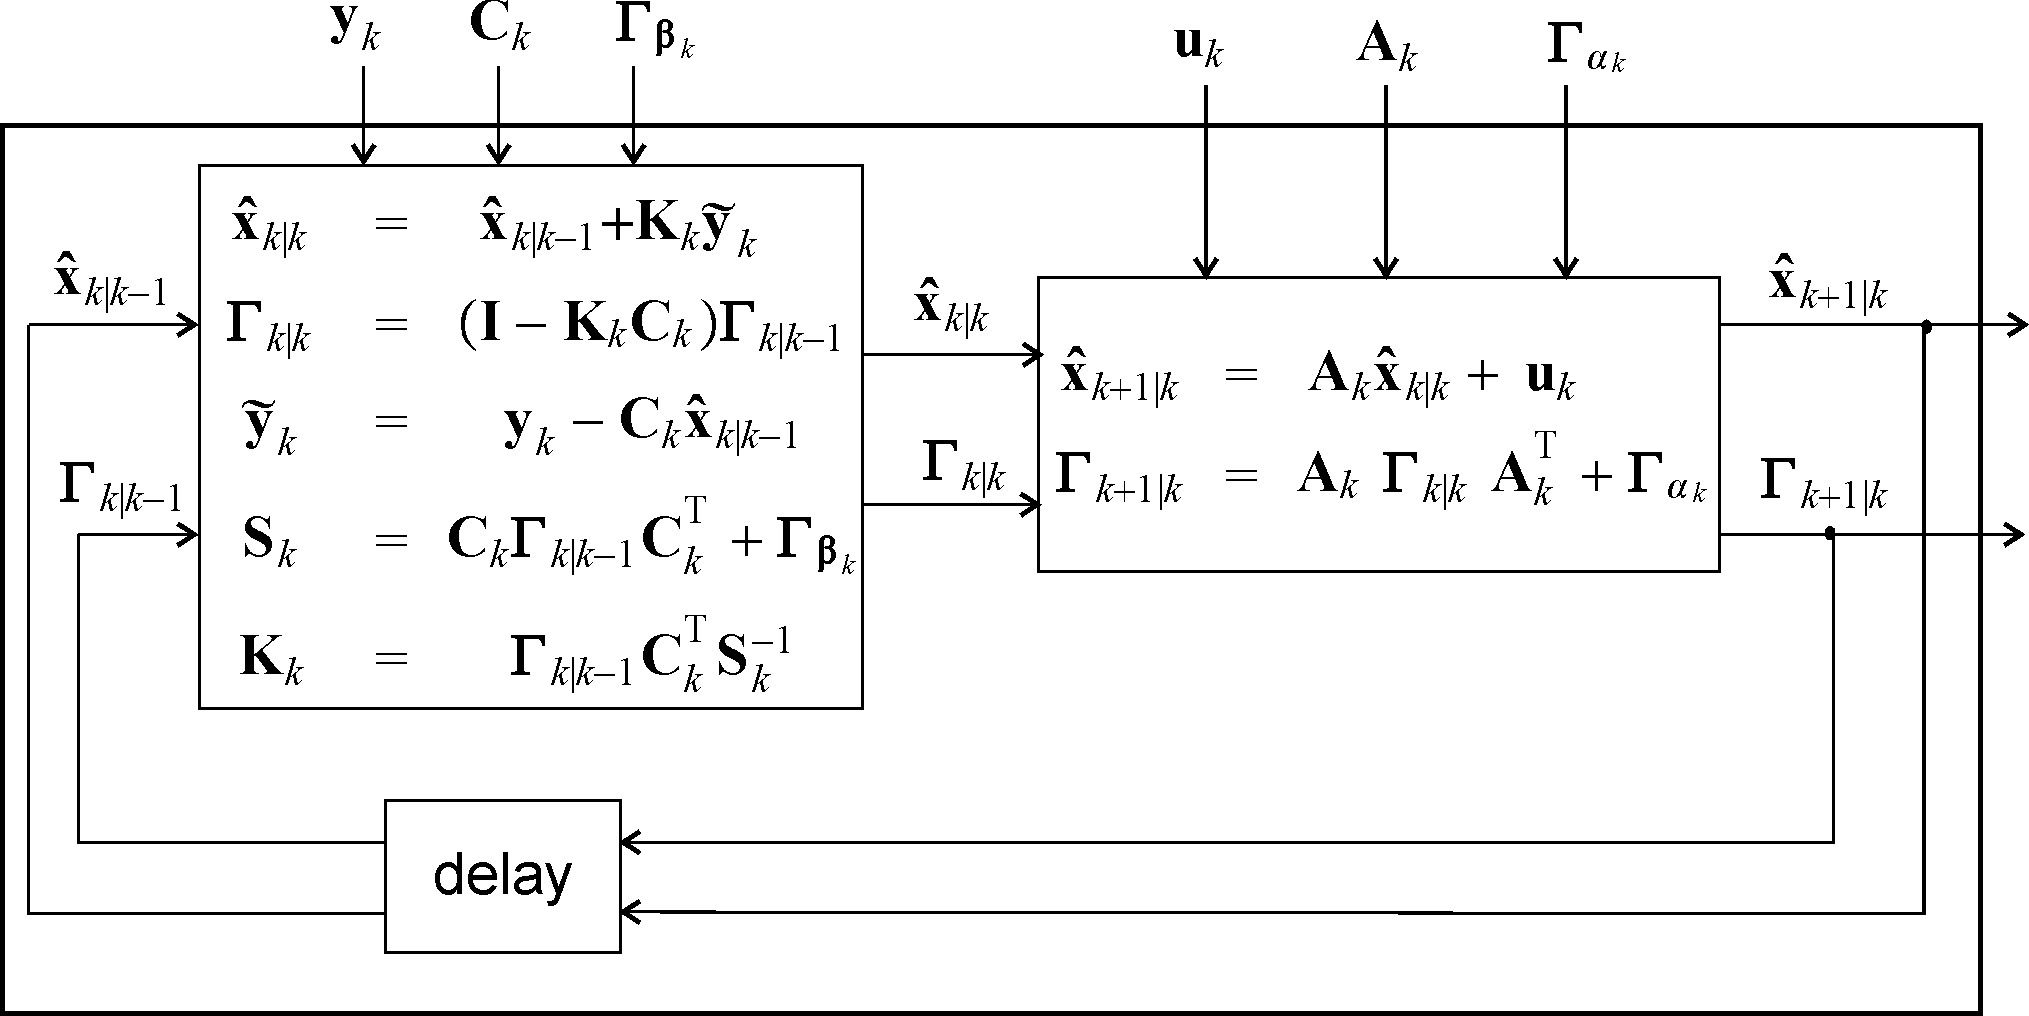
\includegraphics[width=12cm]{kalman_filter_sep_en}\caption{The Kalman filter is composed of a corrector followed by a predictor }

\label{fig:Kalman:filter}
\end{figure}

The function \noun{Kalman} below implements the Kalman filter and
returns $\mathbf{\hat{x}}_{k+1|k},\mathbf{\boldsymbol{\Gamma}}_{k+1|k}$.
In this program, we have the following correspondences: $\mathbf{\hat{x}^{\text{pred}}}\leftrightarrow\mathbf{\hat{x}}_{k|k-1},$
$\boldsymbol{\boldsymbol{\Gamma}}^{\text{pred}}\leftrightarrow\mathbf{\boldsymbol{\Gamma}}_{k|k-1}$
, $\mathbf{\hat{x}^{\text{up}}}\leftrightarrow\mathbf{\hat{x}}_{k|k}$,
$\boldsymbol{\boldsymbol{\Gamma}}^{\text{up}}\leftrightarrow\mathbf{\boldsymbol{\Gamma}}_{k|k}$
(the term \texttt{up} refers to \emph{update}, \emph{i.e.,} correction).\label{algo:kalman}
\begin{singlespace}
\begin{center}
\begin{tabular}{|cl|}
\hline 
 & $\textbf{Function}\ensuremath{\;}\textsc{Kalman }(\mathbf{\hat{x}^{\text{pred}}},\boldsymbol{\boldsymbol{\Gamma}}^{\text{pred}},\mathbf{u},\mathbf{y},\mathbf{\boldsymbol{\Gamma}}_{\mathbf{\boldsymbol{\alpha}}},\mathbf{\boldsymbol{\Gamma}}_{\mathbf{\boldsymbol{\beta}}},\mathbf{A},\mathbf{C})$\tabularnewline
\hline 
1 & $\mathbf{S}:=\mathbf{C}\cdot\boldsymbol{\boldsymbol{\Gamma}}^{\text{pred}}\cdot\mathbf{C}^{\text{T}}+\mathbf{\boldsymbol{\Gamma}}_{\mathbf{\boldsymbol{\beta}}}$\tabularnewline
2 & $\mathbf{K}:=\boldsymbol{\boldsymbol{\Gamma}}^{\text{pred}}\cdot\mathbf{C}^{\text{T}}\cdot\mathbf{S}^{-1}$\tabularnewline
3 & $\widetilde{\mathbf{y}}:=\mathbf{y}-\mathbf{C}\cdot\mathbf{\hat{x}^{\text{pred}}}$\tabularnewline
4 & $\mathbf{\hat{x}^{\text{up}}}:=\mathbf{\hat{x}^{\text{pred}}}\mathbf{+K}\cdot\widetilde{\mathbf{y}}$\tabularnewline
5 & $\boldsymbol{\boldsymbol{\Gamma}}^{\text{up}}:=\left(\mathbf{\mathbf{I}}-\mathbf{K}\cdot\mathbf{C}\right)\boldsymbol{\boldsymbol{\Gamma}}^{\text{pred}}$\tabularnewline
6 & $\hat{\mathbf{x}}^{\text{pred}}:=\mathbf{A}\cdot\mathbf{\hat{x}^{\text{up}}}+\mathbf{u}$\tabularnewline
7 & $\boldsymbol{\boldsymbol{\Gamma}}^{\text{pred}}:=\mathbf{A}\cdot\boldsymbol{\boldsymbol{\Gamma}}^{\text{up}}\cdot\mathbf{A}^{\text{T}}+\mathbf{\boldsymbol{\Gamma}}_{\boldsymbol{\alpha}}$\tabularnewline
8 & Return$\left(\hat{\mathbf{x}}^{\text{pred}},\boldsymbol{\boldsymbol{\Gamma}}^{\text{pred}}\right)$\tabularnewline
\hline 
\end{tabular}
\par\end{center}
\end{singlespace}
\begin{verbatim}

\end{verbatim}
\textbf{Positivity lost}. Due to numerical problems, the covariance
of the innovation $\mathbf{S}_{k}$ can sometimes loose its positivity.
If such a problem arises, it is preferable to replace the corrected
covariance equation by : 
\[
\mathbf{\boldsymbol{\Gamma}}_{k|k}:=\sqrt{\left(\mathbf{\mathbf{I}}-\mathbf{K}_{k}\mathbf{C}_{k}\right)\mathbf{\mathbf{\boldsymbol{\Gamma}}}_{k|k-1}\mathbf{\mathbf{\boldsymbol{\Gamma}}}_{k|k-1}^{\text{T}}\left(\mathbf{\mathbf{I}}-\mathbf{K}_{k}\mathbf{C}_{k}\right)^{\text{T}}}
\]
which will always be positive definite, even when the matrix $\mathbf{\mathbf{\boldsymbol{\Gamma}}}_{k|k-1}$
is not. The Kalman filter equations will then be more stable in the
sense that a slight error on the positive character of the covariance
matrices is removed at the next iteration.

\textbf{Predictor.} When no measurement is available, the Kalman filter
operates in \emph{predictor} mode. In order to be able to use the
Kalman function, $\mathbf{y}$, $\mathbf{\boldsymbol{\Gamma}}_{\mathbf{\boldsymbol{\beta}}},\mathbf{C}$
have to become empty quantities. However, they have to have correct
dimensions in order to perform matrix operations. 

\textbf{Initialization} : Most of the time, we have no idea of the
initial state $\mathbf{x}_{0}$. In this case, we generally set 
\[
\mathbf{\hat{x}}_{0}=\left(0,0,\dots,0\right)\text{ et }\boldsymbol{\Gamma}\mathbf{_{x}}(0)=\left(\begin{array}{llll}
\frac{1}{\varepsilon^{2}} & 0 & 0\\
0 & \frac{1}{\varepsilon^{2}}\\
0 &  & \ddots & 0\\
 &  & 0 & \frac{1}{\varepsilon^{2}}
\end{array}\right),
\]
where $\varepsilon$ in a small positive number (for instance $0.001$).
More or less, this assumption amounts to say that $\mathbf{x}_{0}$
is inside a sphere centered in zero and a radius $\frac{1}{\varepsilon}$.

\textbf{Stationary case}. For time independent systems $\mathbf{\boldsymbol{\Gamma}}_{k+1|k}$
converges to a matrix $\boldsymbol{\Gamma}$. For large $k$ , $\boldsymbol{\Gamma}=\mathbf{\boldsymbol{\Gamma}}_{k+1|k}=\mathbf{\boldsymbol{\Gamma}}_{k|k-1}$.
Thus:
\[
\begin{array}{clcl}
\mathbf{\boldsymbol{\Gamma}}_{k+1|k} & = & \, & \mathbf{A}\cdot\mathbf{\boldsymbol{\Gamma}}_{k|k}\cdot\mathbf{A}^{\text{T}}+\mathbf{\boldsymbol{\Gamma}}_{\boldsymbol{\alpha}}\\
 & = &  & \mathbf{A}\cdot\left(\mathbf{\mathbf{I}}-\mathbf{K}_{k}\mathbf{C}\right)\mathbf{\mathbf{\boldsymbol{\Gamma}}}_{k|k-1}\cdot\mathbf{A}^{\text{T}}+\mathbf{\boldsymbol{\Gamma}}_{\boldsymbol{\alpha}}\\
 & = &  & \mathbf{A}\cdot\left(\mathbf{\mathbf{I}}-\left(\mathbf{\mathbf{\boldsymbol{\Gamma}}}_{k|k-1}\mathbf{C}^{\text{T}}\mathbf{S}^{-1}\right)\mathbf{C}\right)\mathbf{\mathbf{\boldsymbol{\Gamma}}}_{k|k-1}\cdot\mathbf{A}^{\text{T}}+\mathbf{\boldsymbol{\Gamma}}_{\boldsymbol{\alpha}}\\
 & = &  & \mathbf{A}\cdot\left(\mathbf{\mathbf{I}}-\left(\mathbf{\mathbf{\boldsymbol{\Gamma}}}_{k|k-1}\mathbf{C}^{\text{T}}\left(\mathbf{C}\mathbf{\mathbf{\boldsymbol{\Gamma}}}_{k|k-1}\mathbf{C}^{\text{T}}+\mathbf{\boldsymbol{\Gamma}}_{\mathbf{\boldsymbol{\beta}}}\right)^{-1}\right)\mathbf{C}\right)\mathbf{\mathbf{\boldsymbol{\Gamma}}}_{k|k-1}\cdot\mathbf{A}^{\text{T}}+\mathbf{\boldsymbol{\Gamma}}_{\boldsymbol{\alpha}}
\end{array}
\]
Therefore, for large $k$,
\[
\mathbf{\boldsymbol{\Gamma}}=\mathbf{A}\cdot\left(\mathbf{\boldsymbol{\Gamma}}-\mathbf{\boldsymbol{\Gamma}}\cdot\mathbf{C}^{\text{T}}\cdot\left(\mathbf{C}\cdot\mathbf{\mathbf{\boldsymbol{\Gamma}}}\cdot\mathbf{C}^{\text{T}}+\mathbf{\boldsymbol{\Gamma}}_{\mathbf{\boldsymbol{\beta}}}\right)^{-1}\cdot\mathbf{C}\cdot\mathbf{\boldsymbol{\Gamma}}\right)\cdot\mathbf{A}^{\text{T}}+\mathbf{\boldsymbol{\Gamma}}_{\boldsymbol{\alpha}}
\]
which is an equation of Ricatti in $\mathbf{\boldsymbol{\Gamma}}$.
It can be solved by the sequence 
\[
\mathbf{\boldsymbol{\Gamma}}(k+1)\mathbf{=}\mathbf{A}\cdot\left(\mathbf{\boldsymbol{\Gamma}}(k)-\mathbf{\boldsymbol{\Gamma}}(k)\cdot\mathbf{C}^{\text{T}}\cdot\left(\mathbf{C}\cdot\mathbf{\boldsymbol{\Gamma}}(k)\cdot\mathbf{C}^{\text{T}}+\mathbf{\boldsymbol{\Gamma}}_{\mathbf{\boldsymbol{\beta}}}\right)^{-1}\cdot\mathbf{C}\cdot\mathbf{\boldsymbol{\Gamma}}(k)\right)\cdot\mathbf{A}^{\text{T}}+\mathbf{\boldsymbol{\Gamma}}_{\boldsymbol{\alpha}}
\]
up to the equilibrium and starting with $\mathbf{\boldsymbol{\Gamma}}(0)$
large (e.g. $10^{10}\cdot\mathbf{I}$). This computation can be done
before the implementation of the filter, which allows us to avoid
unnecessary real time computation of $\mathbf{\boldsymbol{\Gamma}}_{k+1|k}$.
The corresponding stationary Kalman filter is thus : 
\[
\begin{array}{lll}
\mathbf{\hat{x}}_{k+1|k} & = & \mathbf{A}\mathbf{\hat{x}}_{k|k-1}\mathbf{+\mathbf{A}K}\cdot\left(\mathbf{y}_{k}-\mathbf{C}\mathbf{\hat{x}}_{k|k-1}\right)+\mathbf{u}_{k}\end{array}
\]
with $\mathbf{K}=\mathbf{\mathbf{\boldsymbol{\Gamma}}}\mathbf{C}^{\text{T}}\left(\mathbf{C}\mathbf{\mathbf{\boldsymbol{\Gamma}}}\mathbf{C}^{\text{T}}+\mathbf{\boldsymbol{\Gamma}}\right)^{-1}$.

\chapter*{Exercises}

\rule{0.95\columnwidth}{1pt}

\begin{Exercice} \label{ex:3_equations} Solving three equations
using a Kalman filter \end{Exercice}

\textcolor{blue}{See the correction video at \href{https://youtu.be/Z8x7b1Owdko}{https://youtu.be/Z8x7b1Owdko}}

Let us consider once again the linear equations of Exercise \ref{ex:trois:equations}:
\[
\left\{ \begin{array}{lll}
2x_{1}+3x_{2} & = & 8+\beta_{1}\\
3x_{1}+2x_{2} & = & 7+\beta_{2}\\
x_{1}-x_{2} & = & 0+\beta_{3}
\end{array}\right.
\]
where $\beta_{1},\beta_{2},\beta_{3}$ are three independent, centered
random variables with respective variances $1,4,4$.

1) Solve this system by calling the Kalman filter three times. Give
an estimation of the solution and find the covariance matrix of the
error.

2) Draw the confidence ellipses associated with each call.

3) Compare these with the results obtained for Exercise \ref{ex:trois:equations}.

\rule{0.95\columnwidth}{1pt}

\begin{Exercice} \label{ex:kalman:systdyn:simple} Three-step Kalman
filter \end{Exercice}

\textcolor{blue}{See the correction video at \href{https://youtu.be/beIEAc2QI4s}{https://youtu.be/beIEAc2QI4s}}

Let us consider the discrete-time system: 
\[
\left\{ \begin{array}{lll}
\mathbf{x}_{k+1} & = & \mathbf{A}_{k}\mathbf{x}_{k}+\mathbf{u}_{k}+\mathbf{\boldsymbol{\alpha}}_{k}\\
y_{k} & = & \mathbf{C}_{k}\mathbf{x}_{k}+\beta_{k}
\end{array}\right.
\]
with $k\in\left\{ 0,1,2\right\} $. The values for the quantities
$\mathbf{A}_{k},\mathbf{C}_{k},\mathbf{u}_{k},y_{k}$ are given by:
\[
\begin{tabular}{|c|c|c|c|c|}
\hline  \ensuremath{k}  &  \ensuremath{\mathbf{A}_{k}}  &  \ensuremath{\mathbf{u}_{k}}  &  \ensuremath{\mathbf{C}_{k}}  &  \ensuremath{y_{k}}\\
\hline  \ensuremath{0}  &  \ensuremath{\left(\begin{array}{cc}
0.5 & 0\\
0 & 1
\end{array}\right)}  &  \ensuremath{\left(\begin{array}{c}
8\\
16
\end{array}\right)}  &  \ensuremath{\left(\begin{array}{cc}
1 & 1\end{array}\right)}  &  \ensuremath{7}\\
\hline  \ensuremath{1}  &  \ensuremath{\left(\begin{array}{cc}
1 & -1\\
1 & 1
\end{array}\right)}  &  \ensuremath{\left(\begin{array}{c}
-6\\
-18
\end{array}\right)}  &  \ensuremath{\left(\begin{array}{cc}
1 & 1\end{array}\right)}  &  \ensuremath{30}\\
\hline  \ensuremath{2}  &  \ensuremath{\left(\begin{array}{cc}
1 & -1\\
1 & 1
\end{array}\right)}  &  \ensuremath{\left(\begin{array}{c}
32\\
-8
\end{array}\right)}  &  \ensuremath{\left(\begin{array}{cc}
1 & 1\end{array}\right)}  &  \ensuremath{-6} 
\\\hline \end{tabular}
\]
Let us assume that the signals $\mathbf{\boldsymbol{\alpha}}_{k}$
and $\beta_{k}$ are white Gaussian signals with a unitary covariance
matrix. We have 
\[
\boldsymbol{\Gamma}_{\boldsymbol{\alpha}}=\left(\begin{array}{ccc}
1 &  & 0\\
0 &  & 1
\end{array}\right)\text{ and }\mathbf{\Gamma}_{\mathbf{\beta}}=1.
\]
The initial state vector is unknown and is represented by an estimation
$\mathbf{\hat{x}}_{0|-1}$ and a covariance matrix $\mathbf{\boldsymbol{\Gamma}}_{0|-1}$.
We will take:
\[
\mathbf{\hat{x}}_{0|-1}=\left(\begin{array}{c}
0\\
0
\end{array}\right),\ \mathbf{\boldsymbol{\Gamma}}_{0|-1}=\left(\begin{array}{ccc}
100 &  & 0\\
0 &  & 100
\end{array}\right).
\]
Draw the $\eta=0.9$ confidence ellipses with center $\mathbf{\hat{x}}_{k|k}$
and covariance matrix $\boldsymbol{\Gamma}_{k|k}$ obtained by the
Kalman filter.

\rule{0.95\columnwidth}{1pt}

\begin{Exercice} \label{ex:kalman:moteurcc} Estimating the parameters
of an electric motor \end{Exercice}

\textcolor{blue}{See the correction video at \href{https://youtu.be/_05sBBiw3ac}{https://youtu.be/\_05sBBiw3ac}}

Let us consider once more the DC motor with angular speed $\Omega$
(see Exercises \ref{ex:mc:moteurcc} to \ref{ex:regression:moteurcc}).
We have: 
\[
\Omega=x_{1}U+x_{2}T_{r}
\]
where $U$ is the input voltage, $T_{r}$ is the resistive torque
and $\mathbf{x}=\left(x_{1},x_{2}\right)$ is the vector of parameters
to estimate. The following table presents the measurements obtained
for various experimental conditions:
\[
\begin{tabular}{|c|c|c|c|c|c|}
\hline  \ensuremath{k}  &  \ensuremath{0}  &  \ensuremath{1}  &  \ensuremath{2}  &  \ensuremath{3}  &  \ensuremath{4}\\
\hline  \ensuremath{U(\text{V})}  &  \ensuremath{4}  &  \ensuremath{10}  &  \ensuremath{10}  &  \ensuremath{13}  &  \ensuremath{15}\\
\hline  \ensuremath{T_{r}(\text{Nm})}  &  \ensuremath{0}  &  \ensuremath{1}  &  \ensuremath{5}  &  \ensuremath{5}  &  \ensuremath{3}\\
\hline  \ensuremath{\Omega(}rad\ensuremath{/\sec)}  &  \ensuremath{5}  &  \ensuremath{10}  &  \ensuremath{11}  &  \ensuremath{14}  &  \ensuremath{17} 
\\\hline \end{tabular}
\]
We still assume that the variance of the measurement error is equal
to 9 and that $x_{1}\simeq1$ and $x_{2}\simeq-1$ with a variance
of $4$. Using the Kalman filter, calculate an estimation of the parameters
$x_{1},x_{2}$ and give the associated covariance matrix.

\rule{0.95\columnwidth}{1pt}

\begin{Exercice} \label{ex:kalman:temperature} Temperature estimation
\end{Exercice}

\textcolor{blue}{See the correction video at \href{https://youtu.be/6sTAJvH3PO8}{https://youtu.be/6sTAJvH3PO8}}

The temperature in a room has to verify (after temporal discretization)
the state equation: 
\[
\left\{ \begin{array}{lll}
x_{k+1} & = & x_{k}+\alpha_{k}\\
y_{k} & = & x_{k}+\beta_{k}
\end{array}\right.
\]
We assume that the state noise $\alpha_{k}$ and the measurement noise
$\beta_{k}$ are independent and Gaussian with covariance $\Gamma_{\alpha}=4$
and $\Gamma_{\beta}=3$.

1) Give the expression of the Kalman filter that allows to estimate
the temperature $x_{k}$ from the measurement $y_{k}$. From this
deduce an expression of $\hat{x}_{k+1|k}$ and $\Gamma_{k+1|k}$ in
function of $\hat{x}_{k|k-1},\Gamma_{k|k-1}$,$y_{k}$.

2) For large enough $k$, we may assume that $\Gamma_{k+1|k}=\Gamma_{k|k-1}=\Gamma_{\infty}$.
We then obtain the so-called\emph{ asymptotic} Kalman filter. Give
the expression of the asymptotic Kalman filter. How would you characterize
the precision of this filter ?$~$

3) Going back to the non-asymptotic case, but now assuming that $\Gamma_{\alpha_{k}}=0$,
what is the value of $\Gamma_{\infty}$ ? Discuss.


\chapter{Localization \label{ch:localisation}}

Localization consists of finding the position of the robot (\emph{i.e.},
the coordinates of its center as well as its orientation), or more
generally all its degrees of freedom. This problem is encountered
in navigation, where we need to approximate the position, orientation
and speed of the robot. The problem of localization is often considered
to be a particular case of state estimation, which will be presented
in the following chapters. However, in the case where an accurate
state model is not available for our robot, an instantaneous localization
often remains possible and may be sufficient for making a decision.
Let us take for instance the situation in which we are aboard a ship
and have just detected a lighthouse whose absolute position and height
are known. By measuring the perceived height of the lighthouse and
its angle relative to the ship, we may deduce the position of the
ship using a compass and this, without using a state model for the
ship. Instantaneous, or \emph{model-free} localization is an approach
to localization that does not utilize the evolution equation of the
robot, \emph{i.e.}, it does not seek to make the measures coherent
through time. This localization mainly consists of solving equations
of geometric nature which are often nonlinear. The variables involved
may be position variables or kinematic variables such as speed or
accelerations. Since these localization methods are specific and quite
far from state estimation methods, we will devote an entire chapter
to them. After introducing the main sensors used for localization,
we will present goniometric localization (in which the robot uses
the angles of perception of landmarks) followed by multilateration
which uses distances between the robot and the landmarks.

\section{Sensors}

The robots are equipped with numerous sensors that are used for their
localization. We will now present some of these.

\textbf{Compass.} It measures the magnetic field of its environment.
If no magnetic disturbance exists, we get the magnetic north. In practice
magnetic disturbances exists in the robot and a calibration procedure
is required to compensate the hard-iron and soft-iron disturbances.

\textbf{Odometers}. Robots with wheels are generally equipped with
odometers that measure the angular movements of the wheels. Given
only the odometers, it is possible to calculate an estimation of the
position of the robot. The precision of such a localization is very
low given the systematic integration of the estimation error. We say
that the estimation is drifting.

\textbf{Doppler log}.This type of sensor, mainly used in underwater
robotics, allows to calculate the speed of the robot. A Doppler log
emits ultrasounds that are reflected by the ocean bed. Since the ocean
bed is immobile, the sensor is able to estimate the speed of the robot
by using the Doppler effect with a very high precision (around $0.1$
$m/s$).

\textbf{Accelerometers}. These sensors provide measurements of the
instantaneous forward acceleration. The principle of the axis-based
accelerometer is illustrated on Figure \ref{fig:accelero}. Generally,
three accelerometers are used by the robot. Due to gravity, the value
measured according to the vertical axis must be compensated.

\begin{figure}[H]
\centering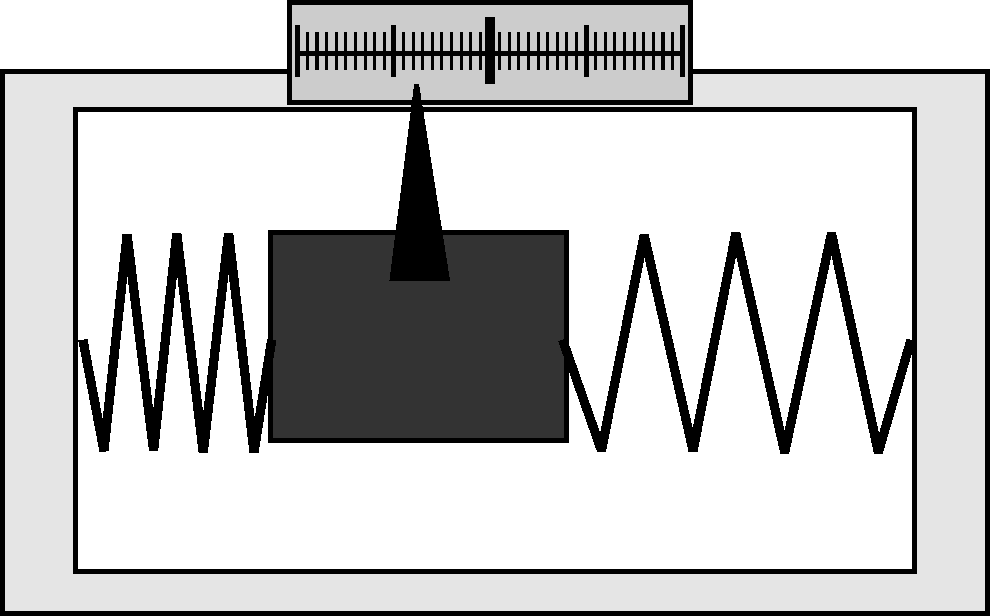
\includegraphics[width=6cm]{accelero}\caption{Operating principle of an accelerometer}

\label{fig:accelero}
\end{figure}

\textbf{Gyros}. A gyro provides measurements of the instantaneous
rotation speed. There are three types of gyros: the Coriolis vibratory
gyro, the mechanical gyro and the optical gyro. The principle of the
Coriolis vibratory gyro is illustrated on the left of Figure \ref{fig:gyro}.
A vertical rod placed on a horizontal disk vibrates from left to right.
As a result of the Coriolis force, if the disk rotates there is an
angular vibration following the axis of the rod whose amplitude allows
to get the rotation speed of the disk. If the disk is not rotating,
there is a forward rotation, but it is not angular. Piezoelectric
gyros, very widely used for low-cost robotics, form a subclass of
Coriolis vibratory gyroscopes. These gyros exploit the variation of
the amplitude of a piezoelectric oscillator induced by the Coriolis
force, due to the rotation applied to the sensor. Mechanical gyros
make use of the fact that a rotating body tends to preserve its rotational
axis if no torque is subjected to it. A well-known example is the
gimbal gyroscope invented by Foucault, represented on the right side
of Figure \ref{fig:gyro}. A flywheel at the center rotates with high
speed. If the base of the gyroscope moves, the two gimbal angles $\psi,\theta$
will change, but the rotation axis of the flywheel will not. From
the values of $\psi,\theta,\dot{\psi},\dot{\theta}$, we can find
the rotation speed of the base (which is fixed on the robot). If the
rotation axis of the flywheel is initialized correctly, and in a perfect
situation in which no torque is exerted on this flywheel, such a system
would theoretically give us the orientation of the robot. Unfortunately,
there is always a small drift and only the rotation speed can be given
in a reliable and drift-free way.

\begin{figure}[H]
\centering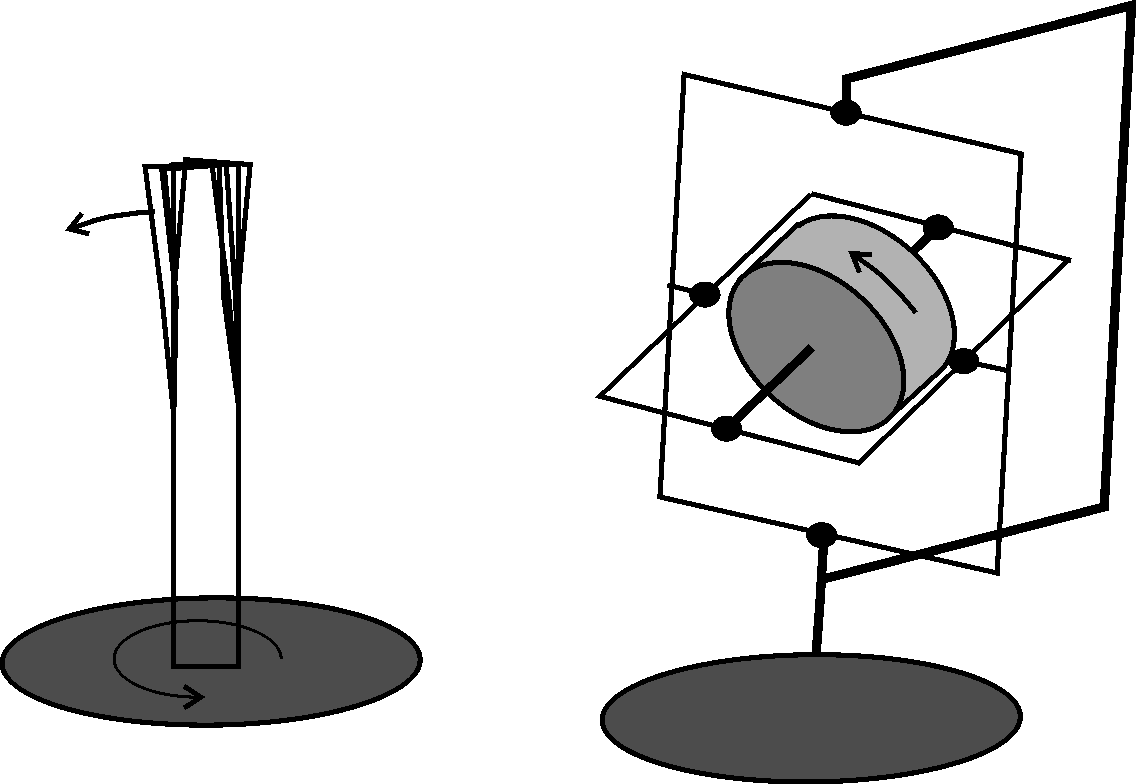
\includegraphics[width=7cm]{gyro}\caption{Coriolis vibratory gyroscope and gimbal gyroscope}

\label{fig:gyro}
\end{figure}

More recent, optical gyroscopes can be as precise as mechanical ones.
They make use of the Sagnac effect (for a circular optical path, the
time taken by light to make a complete lap depends on the direction
of the path) and have a precision of around $0.001$ deg/s. Their
principle is illustrated in Figure \ref{fig:sagnac}. On figure (a),
the laser leaves the light source represented by the black disk. On
figure (b), the beam splitter creates two other beams which travel
in opposite directions in the optical loop. After rebounding several
times on the three mirrors represented in grey, the two beams meet.
Since the beams intersect on the left, the gyro rotates in the opposite
trigonometric direction (c). The beams are separated again on figure
(d). The two beams that arrive at the receiver are not in phase. Their
phase offset allows to find the rotation speed of the gyro, which
is fixed on the robot.

\textbf{IMU.\ }An \emph{inertial measurement unit} associates a gyro
and an accelerometer in order to increase the precision of the estimation.
More recent ones merge other types of information such as the estimated
speed or even take into account Earth's rotation. Thus, they may deduce
the direction of the Earth's North-South axis in the robot's coordinate
system. Knowing this direction gives us two equations involving the
Euler angles of the robot which are the bank $\phi,$ the elevation
$\theta$ and the heading $\psi$ of the robot, expressed in a local
coordinate system. Due to the accelerometer included in the unit,
it is possible to deduce the gravity vector from the above and thus
to generate an additional equation which will allow to calculate the
three Euler angles. Let us note that the accelerometers also give
us the accelerations in all directions (the \emph{surge} in the direction
of the robot, the \emph{heave} (in the vertical direction), the \emph{sway}
for lateral accelerations). The knowledge of the gravity vector and
the axis of rotation theoretically allows, using a simple scalar product,
to find the latitude of the robot. However, the obtained precision
is too low to be taken into account in localization.

\begin{figure}[H]
\centering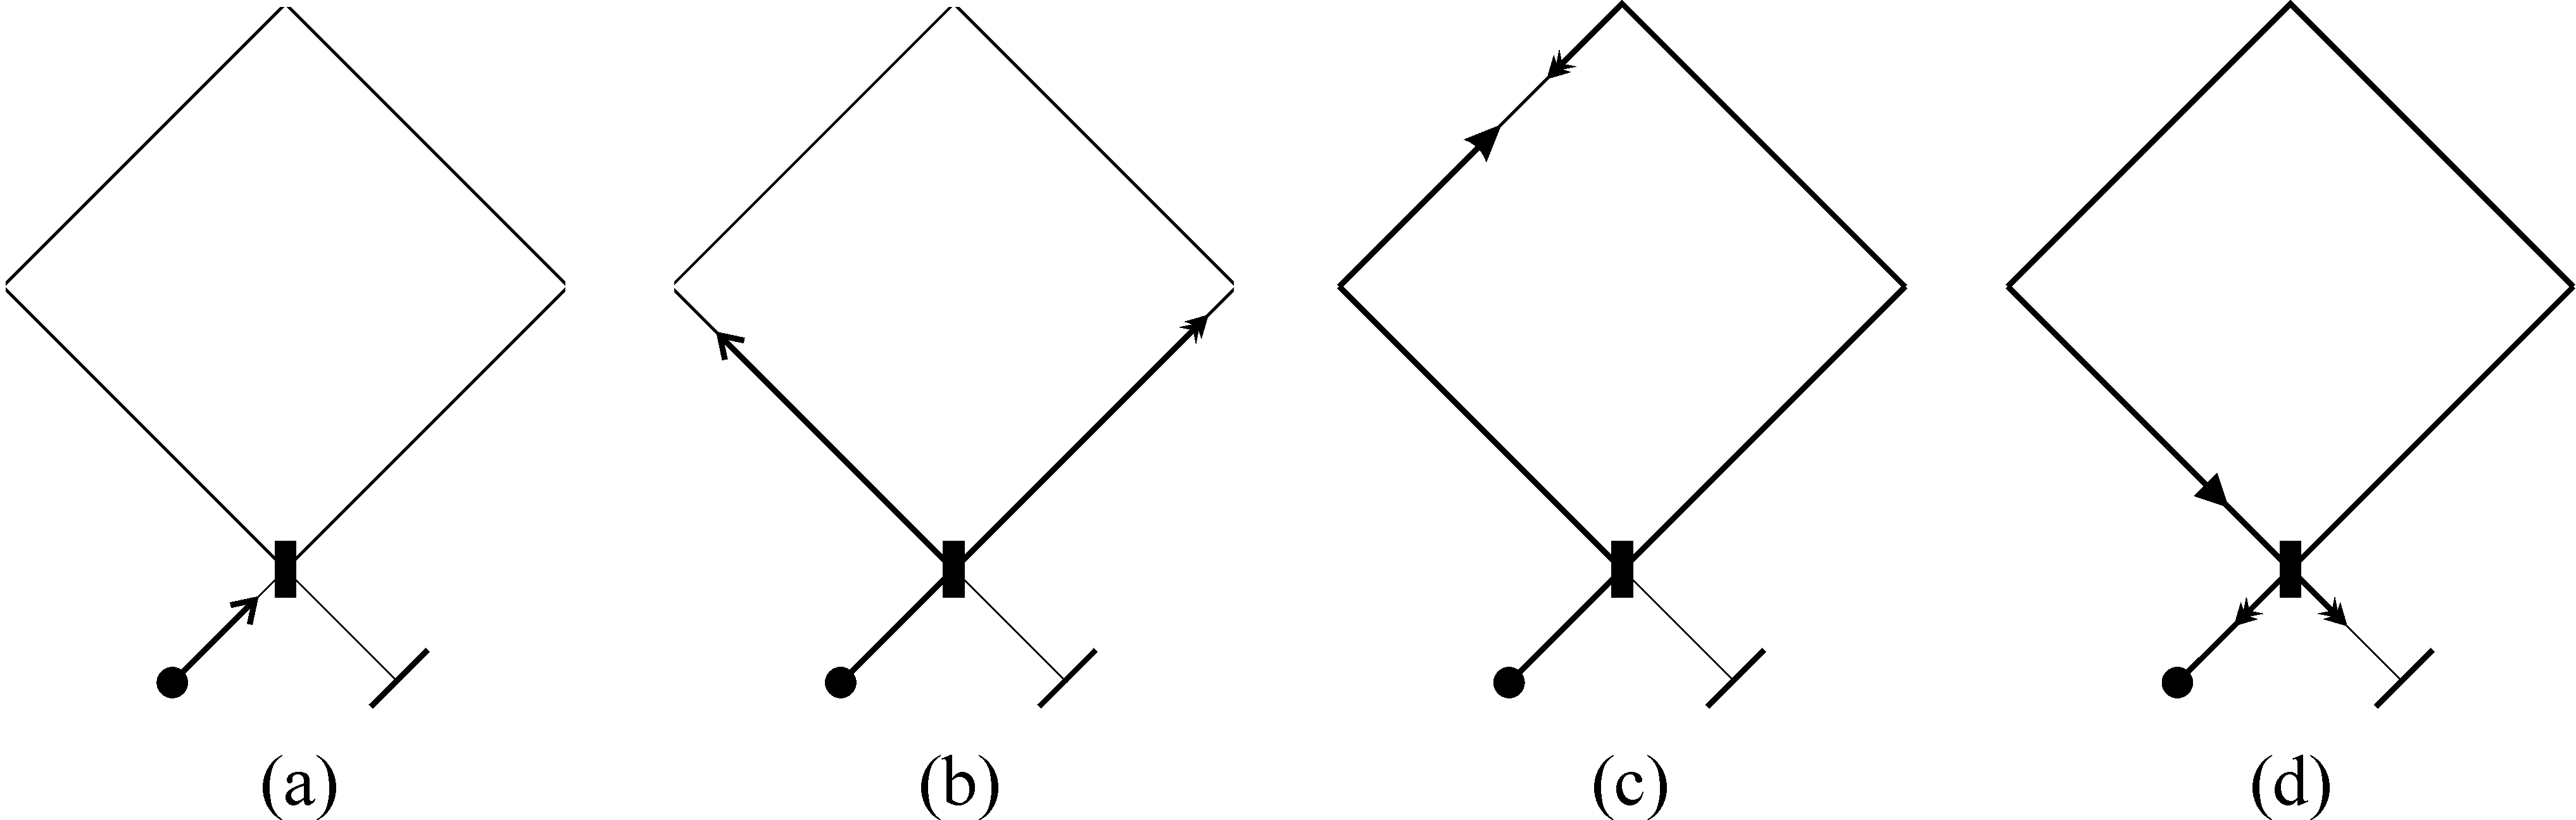
\includegraphics[width=12cm]{sagnac}\caption{Principle of the Sagnac effect for optical gyroscopes}

\label{fig:sagnac}
\end{figure}

\textbf{Barometer}.\index{barometer} It measures pressure. In the
case of underwater robots, it allows to deduce the depth of the robot
with a precision of 1~cm. For indoor flying robots, the barometer
is used to measure the altitude with a precision of around one meter.

\textbf{GPS} (\emph{Global Positioning System}) or \textbf{GNSS} (\emph{Global
Navigation Satellite System}) is a satellite navigation system that
provides a geolocalization service covering the entire world. Nowadays,
the American NAVSTAR system (\emph{NAVigation System by Timing And
Ranging}) and the Russian GLONASS system (GLObalnaya NAvigazionnaya
Sputnikovaya Sistema) are operational. Two other systems are being
developed: the Chinese \emph{Compass} system and the European \emph{Galileo}
system. In practice, our mobile robots will use the American system,
operational since 1995, that we will refer to as GNSS. Originally
designed for exclusive military use, the precision of civil applications
was limited to several hundreds of meters by a deliberate degradation
of civil signals. The deactivation of this degradation in 2000 allowed
the precision to increase to about ten meters. Given that electromagnetic
waves (here around 1.2 MHz) do not propagate under water or across
walls, the GNSS does not work within buildings or in water. Thus,
during a diving experiment, an underwater robot can only be localized
by GNSS when it begins its dive or when it resurfaces. When a georeferenced
station is near the robot and advises it about the errors in distance
calculated for each satellite, a localization with a precision of
$\pm1~$m is possible. This operating mode forms the so-called differential
GPS or DGPS. Finally, by using the phase, it us possible to achieve
even a centimeter precision. This is the principle of the \emph{kinematic
GPS}\index{kinematic GPS}. A detailed and educational presentation
of the GNSS can be found in the thesis of Vincent Drevelle \cite{DrevelleThese}.
In practice, a GNSS gives us a longitude $\ell_{x}$ and a latitude
$\ell_{y}$ and it is often comfortable to convert it to Cartesian
coordinates in a local coordinate system $(\mathbf{o,i},\mathbf{j},\mathbf{k})$
fixed within the area in which the robot is evolving. Let us denote
by $\ell_{x}^{0}$ and $\ell_{y}^{0}$ the longitude and the latitude
expressed in radians at the origin $\mathbf{o}$ of this coordinate
system. We will assume that the vector $\mathbf{i}$ indicates the
North, $\mathbf{j}$ indicates the East and $\mathbf{k}$ is oriented
towards the center of the Earth. Let $\mathbf{p}=(p_{x},p_{y},p_{z})$
be the coordinates of the robot expressed in the coordinate system
$(\mathbf{o,i},\mathbf{j},\mathbf{k})$. From the latitude and longitude
given by the GNSS, we can deduce the first two coordinates of the
robot, expressed in meters in the local coordinate system, by using
the following relation: 
\[
\left(\begin{array}{l}
p_{x}\\
p_{y}
\end{array}\right)=\rho\left(\begin{array}{ccc}
0 & \, & 1\\
\cos\ell_{y} &  & 0
\end{array}\right)\left(\begin{array}{c}
\ell_{x}-\ell_{x}^{0}\\
\ell_{y}-\ell_{y}^{0}
\end{array}\right)=\left(\begin{array}{c}
\rho~\left(\ell_{y}-\ell_{y}^{0}\right)\\
\rho\cos\ell_{y}\cdot\left(\ell_{x}-\ell_{x}^{0}\right)
\end{array}\right)
\]
where $\rho$ corresponds to the distance between $\mathbf{o}$ and
the center of the Earth ($\rho\simeq6~371~$km, if $\mathbf{o}$ is
not too far from sea level). This formula is valid everywhere on Earth,
if we assume that the Earth is spherical and if the robot is in the
neighborhood of the origin $\mathbf{o}$ (let us say a distance inferior
to 100~km). In order to understand this formula, we must note that
$\rho\cos\left(\ell_{y}\right)$ corresponds to the distance between
$\mathbf{o}$ and the rotational axis of the Earth. Thus, if a robot
is moving on a latitude parallel $\ell_{y}$, by modifying its longitude
by an angle $\alpha>0$, it will have traveled $\alpha\rho\cos\ell_{y}$
meters. Similarly, if this robot is moving on a meridian with an angle
$\beta$ in latitude, it will have traveled $\beta\rho$ meters.

\textbf{Radar or sonar. }The robot emits electromagnetic or ultrasound
waves. It recovers their echoes and builds an image that it interprets
in order to map its surroundings. The radar is mainly used by surface
or flying robots. The sonar is used as a low-cost rangefinder by robots
with wheels as well as in underwater robotics.

\textbf{Lidar}. It composed of an emitter, projecting laser beams,
and a receiver measuring the time-of-flight. Underwater, green lasers
are used to get a lower absorption.

\textbf{Cameras}. Cameras are low-cost sensors used for the recognition
of objects. They are also used as goniometers by finding angles relative
to landmarks that will then be used for localization.

\section{Goniometric localization}

\subsection{Formulation of the problem}

The problem consists of using angles measured between the robot and
the landmarks, whose position as a function of time is known, for
localization. Let us consider the robot in Figure \ref{fig:etastriangule}
moving on a plane. We call \emph{bearing} the angle $\alpha_{i}$
between the axis of the robot and the vector pointing towards the
landmark. These angles could have been obtained, for instance, using
a camera.

\begin{figure}[H]
\centering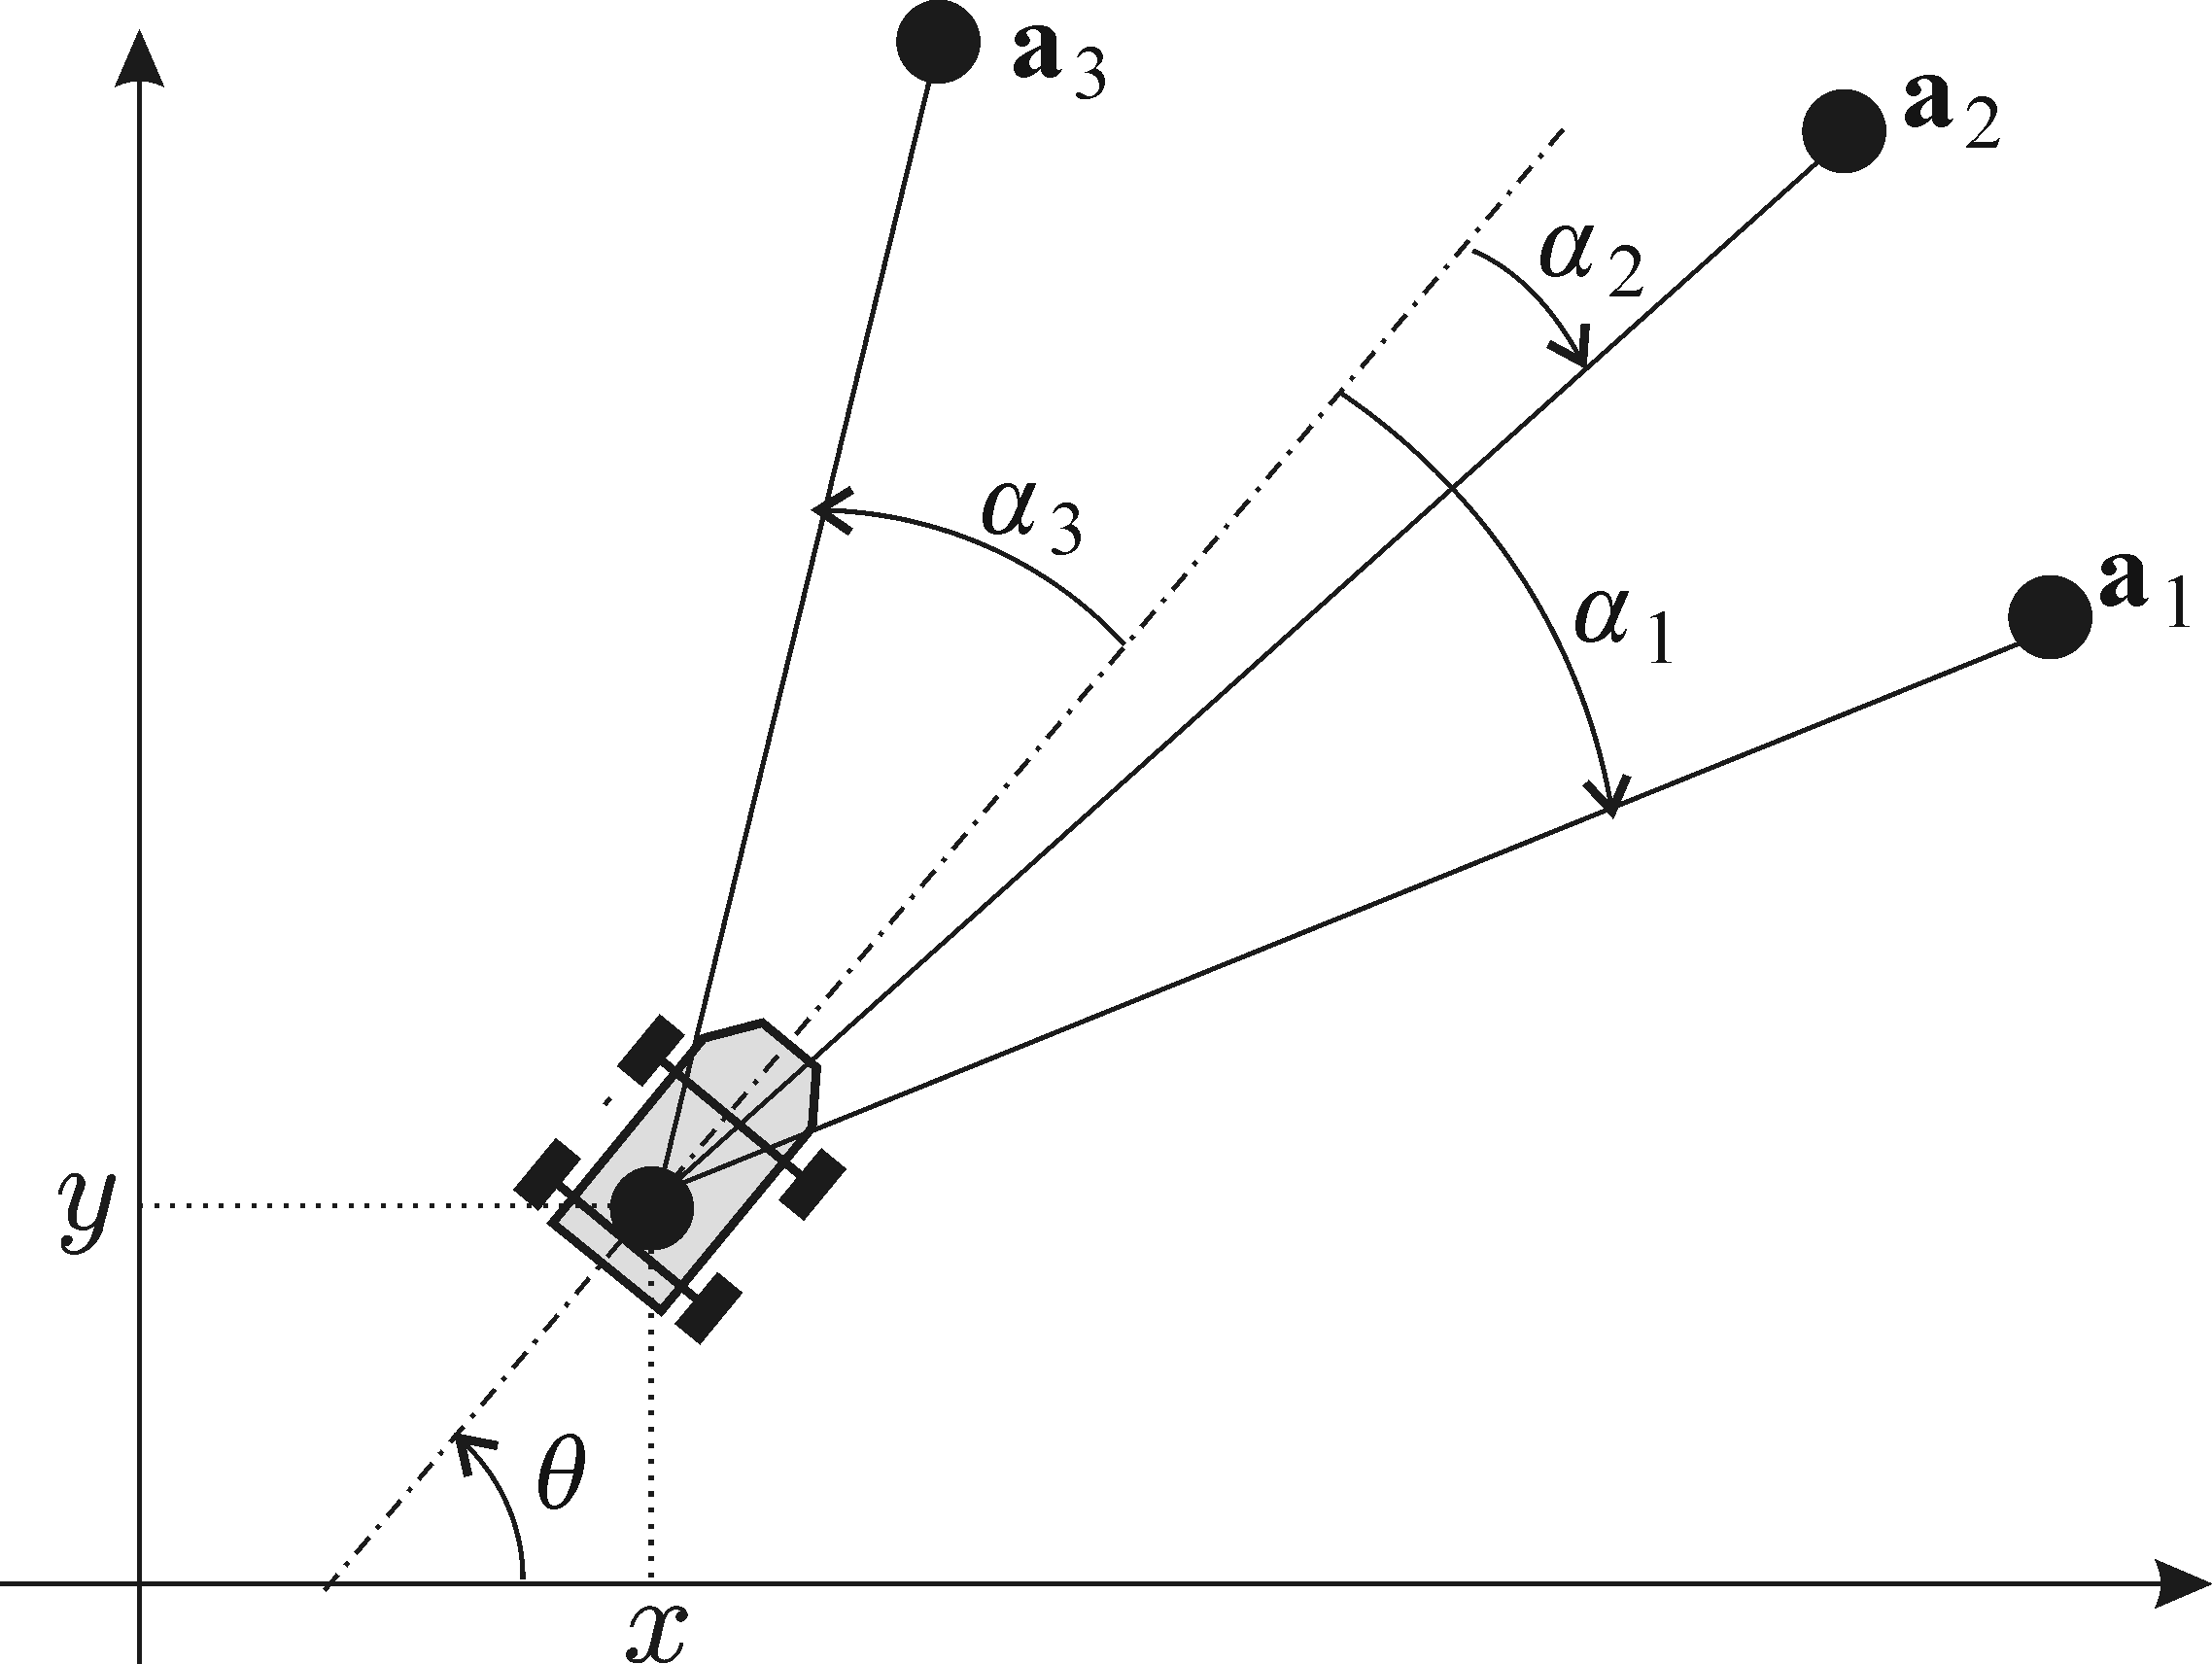
\includegraphics[width=7.5cm]{etastriangule}\caption{A robot moving on a plane, measures the angles in order to locate
itself}

\label{fig:etastriangule}
\end{figure}

Recall that two vectors $\mathbf{u},\mathbf{v}$ of $\mathbb{R}^{2}$
are collinear if their determinant is zero, \emph{i.e.}, if $\det\left(\mathbf{u},\mathbf{v}\right)=0$.
Thus, for each landmark, we have the relation: 
\[
\begin{array}{lll}
\det\left(\left(\begin{array}{c}
x_{i}-x\\
y_{i}-y
\end{array}\right),\left(\begin{array}{c}
\cos\left(\theta+\alpha_{i}\right)\\
\sin\left(\theta+\alpha_{i}\right)
\end{array}\right)\right) & = & 0\end{array},
\]
\emph{i.e.}, 
\begin{equation}
\begin{array}{lll}
\left(x_{i}-x\right)\sin\left(\theta+\alpha_{i}\right)-\left(y_{i}-y\right)\cos\left(\theta+\alpha_{i}\right) & = & 0,\end{array}\label{eq:relation:angle}
\end{equation}
where $(x_{i},y_{i})$ are the coordinates of the landmark $\mathbf{a}_{i}$
and $\theta$ is the robot's heading.

\subsection{Inscribed angles\index{inscribed angles}}
\begin{thm}
\textbf{(Inscribed Angle)} Consider a triangle $\mathbf{abm}$ as
represented on Figure \ref{fig:arc_capable_th}. Let us denote by
$\mathbf{c}$ the center of the circle circumscribed to this triangle
(\emph{i.e.}, $\mathbf{c}$ is at the intersection of the three perpendicular
bisectors). Let $\alpha=\widehat{\mathbf{amc}}$, $\beta=\widehat{\mathbf{cmb}}$,
$\gamma=\widehat{\mathbf{acb}}$. We have the angular relation: 
\[
\gamma=2\left(\alpha+\beta\right).
\]
\end{thm}
\begin{figure}[H]
\centering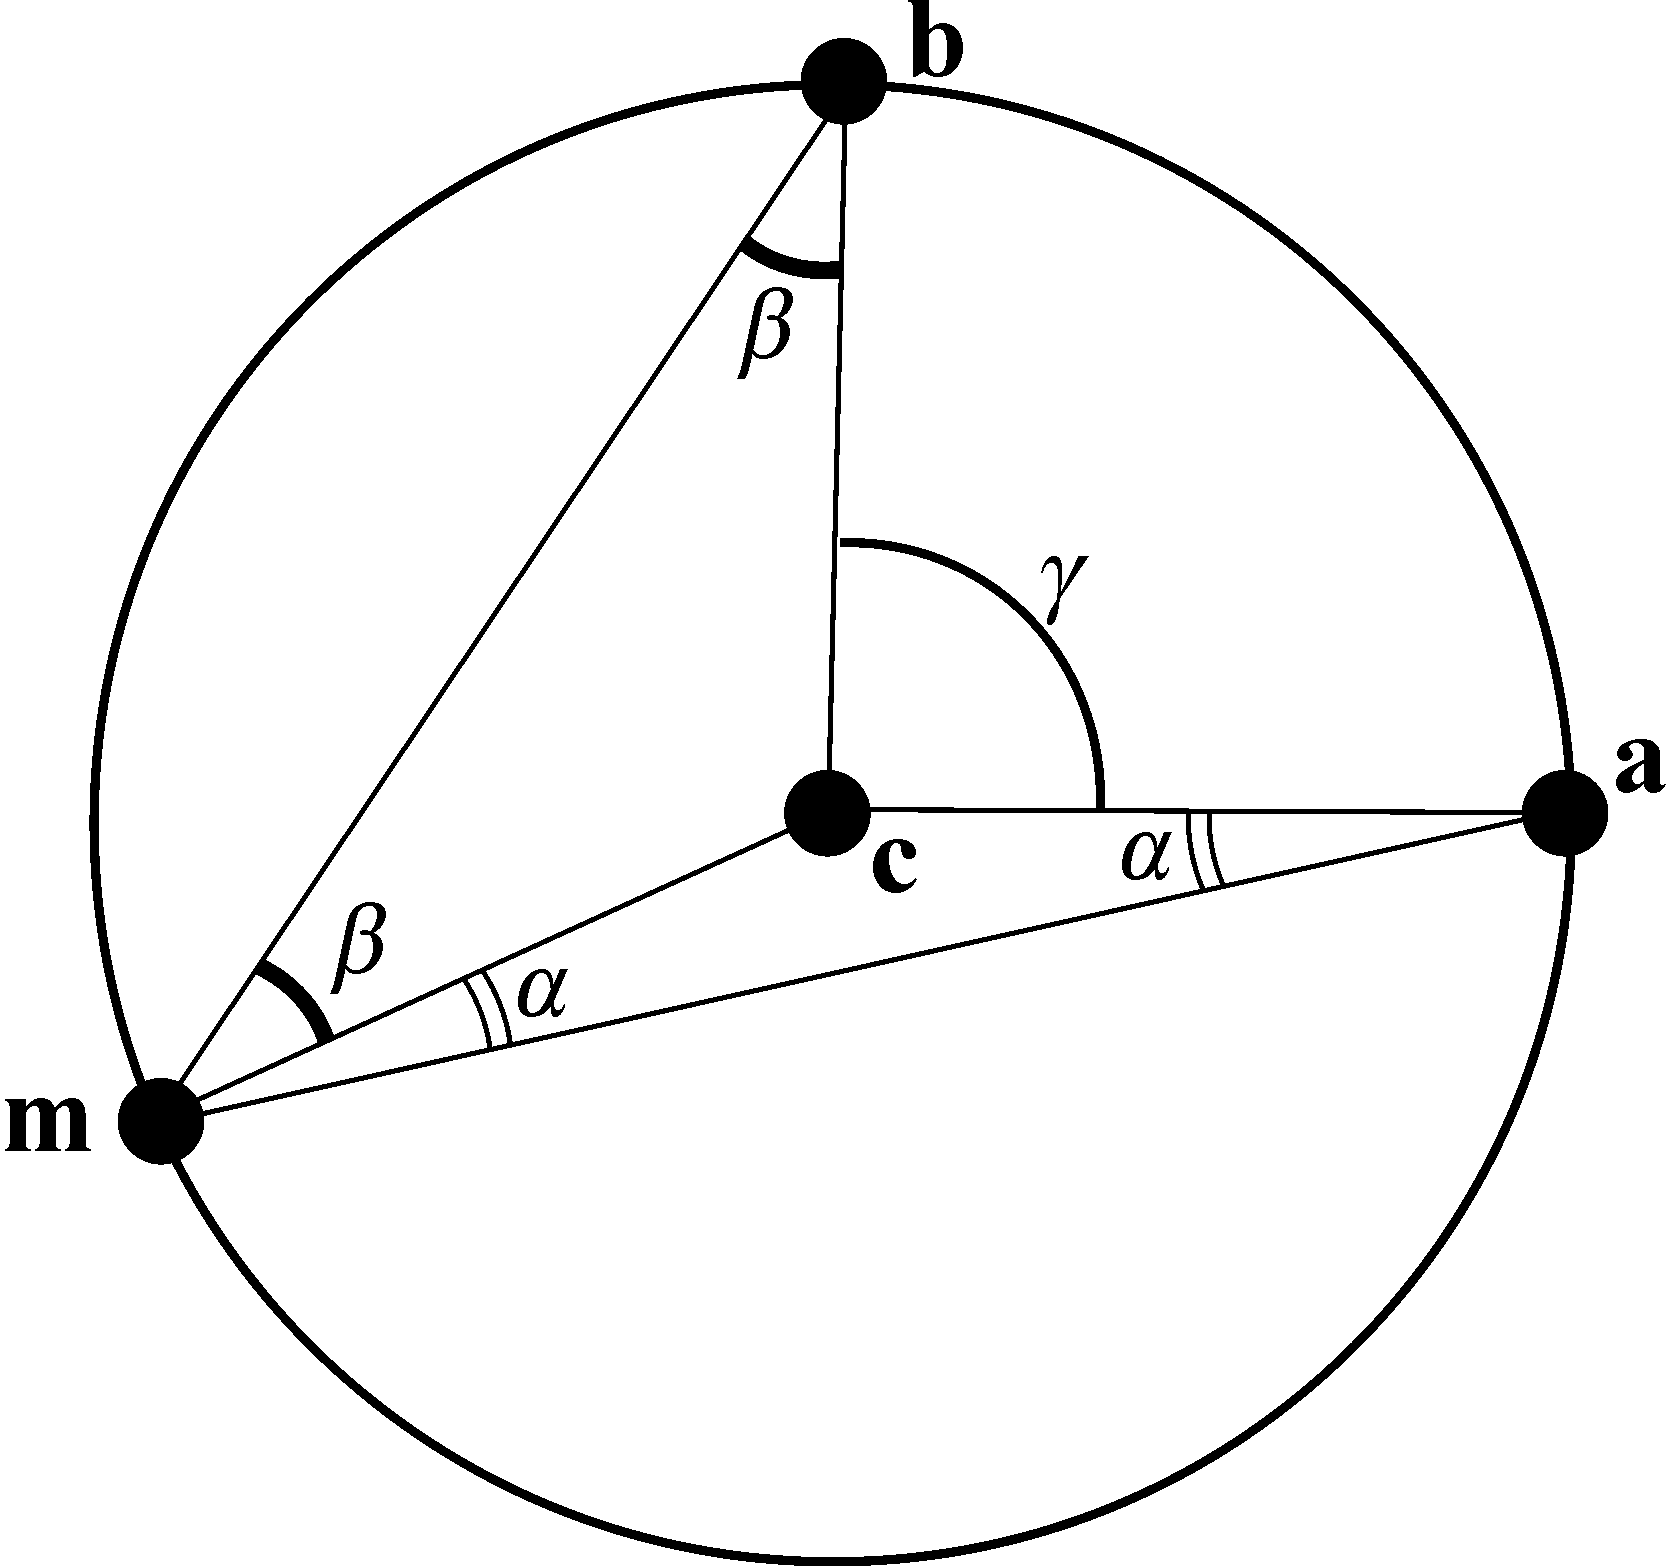
\includegraphics[width=7cm]{arc_capable_th}\caption{Illustration of the Inscribed Angle Theorem}

\label{fig:arc_capable_th}
\end{figure}

\begin{proof}
\noindent Since the two triangles $\mathbf{amc}$ and $\mathbf{cmb}$
are isosceles. We thus find the angles $\alpha$ and $\beta$ as shown
on the figure. By going around the point $\mathbf{c}$ we obtain:
\[
\gamma+\left(\pi-2\beta\right)+\left(\pi-2\alpha\right)=2\pi.
\]
Thus $\gamma=2\alpha+2\beta.$
\end{proof}
A consequence of this theorem is that if $\mathbf{m}$ moves on the
circle, the angle $\alpha+\beta$ will not move.

\textbf{Inscribed arcs}. Let us consider two points $\mathbf{a}_{1}$
and $\mathbf{a}_{2}$. The set of points $\mathbf{m}$ such that the
angle $\widehat{\mathbf{a}_{1}\mathbf{ma}_{2}}$ is equal to $\alpha$
is a circle arc, referred to as an \emph{inscribed arc}\index{inscribed arc}.
We can show this from Relations (\ref{eq:relation:angle}) or from
the Inscribed Angle Theorem. Goniometric localization often breaks
down to intersecting arcs. Figure \ref{fig:arc_capable} illustrates
the concept of an inscribed arc.

\begin{figure}[H]
\centering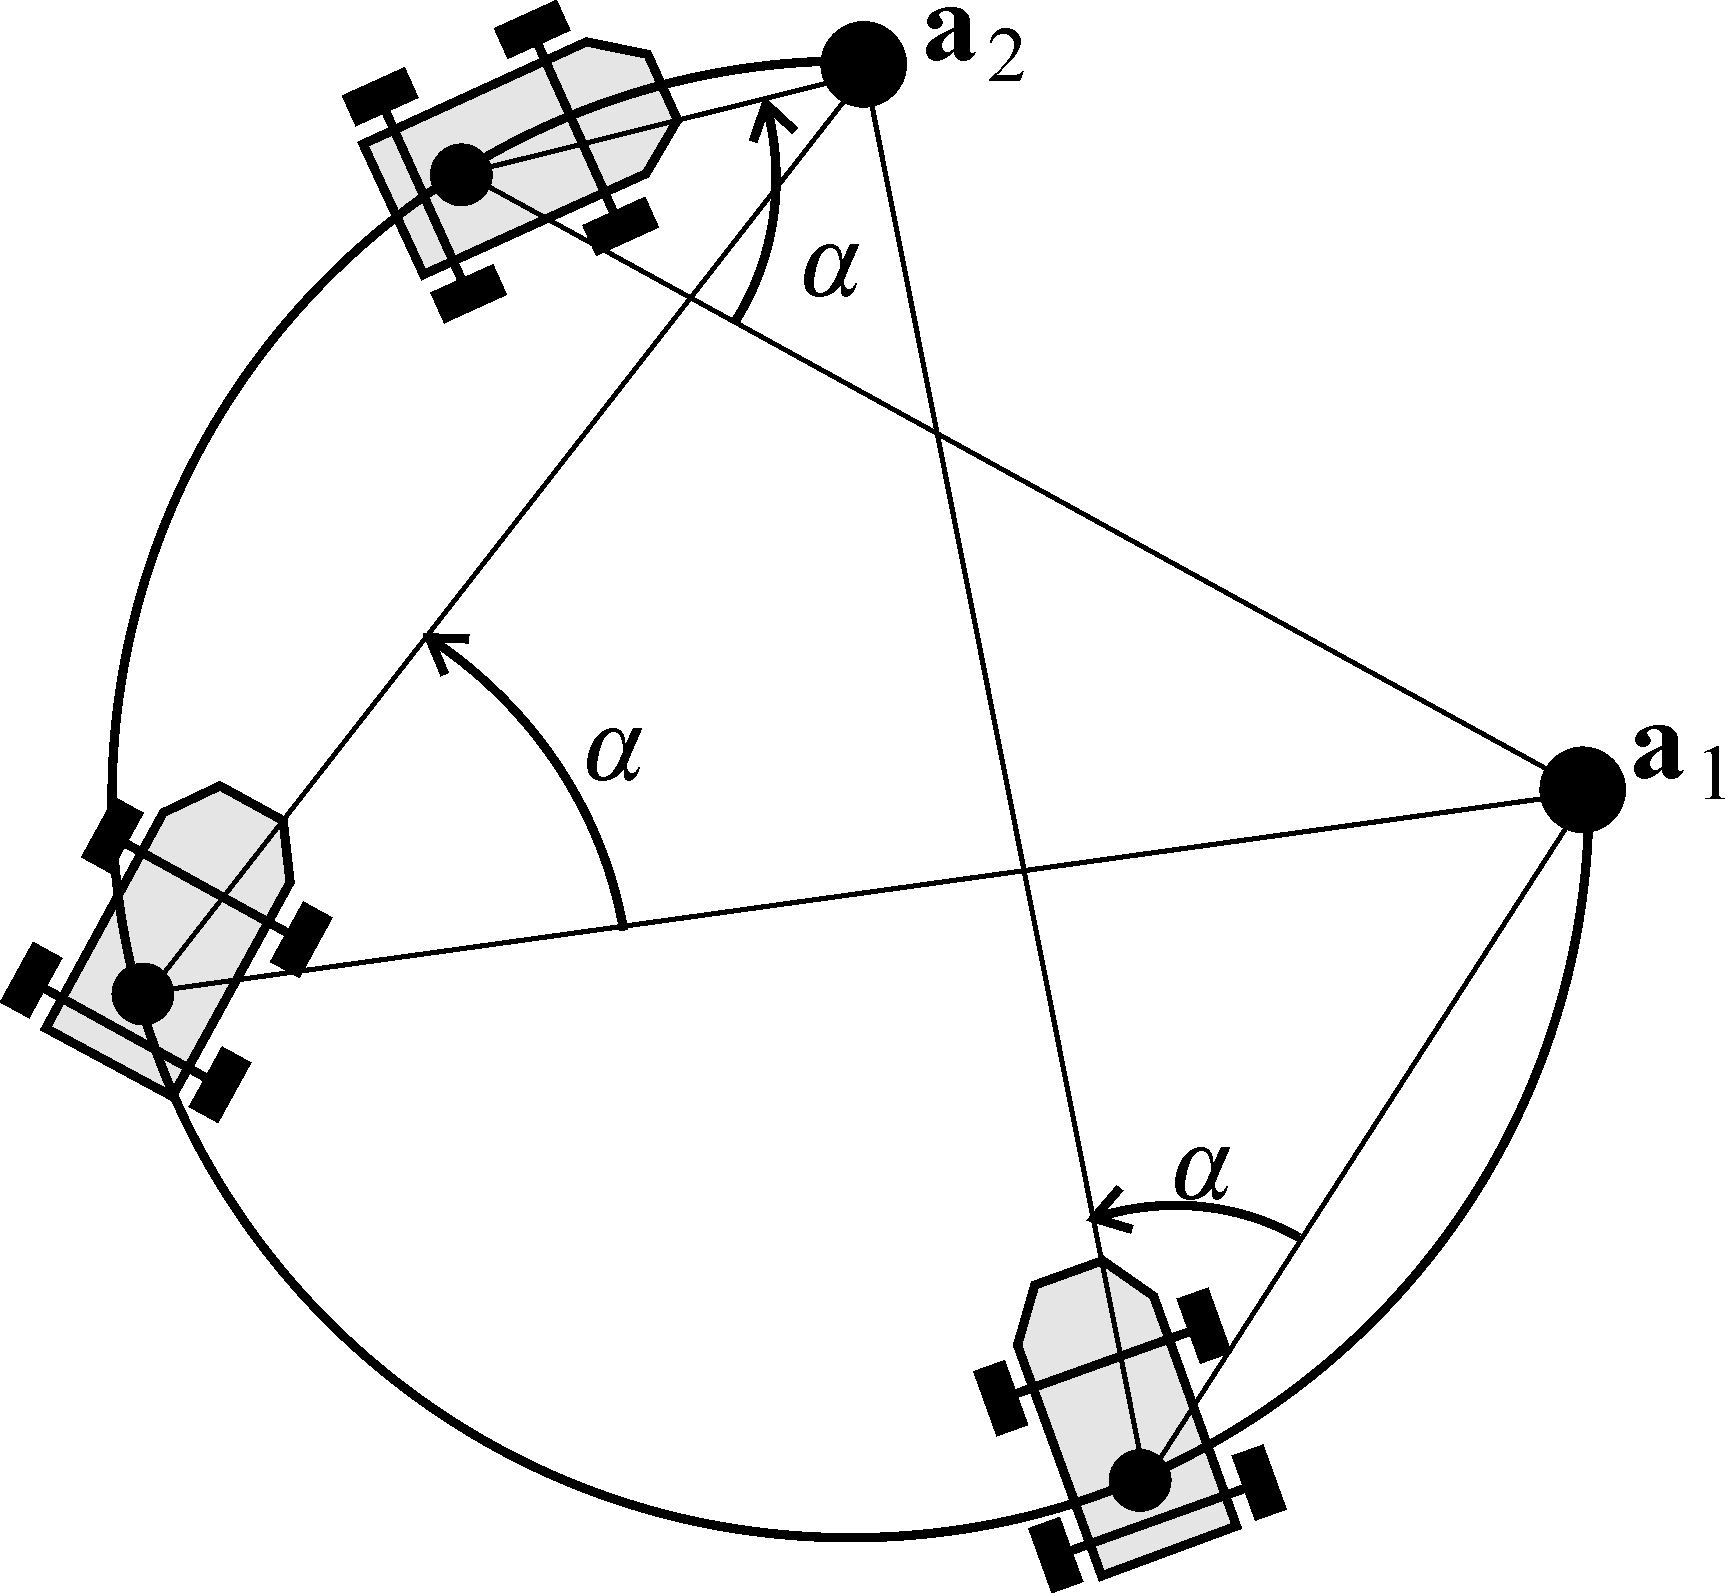
\includegraphics[width=7cm]{arc_capable}\caption{The three cars perceive the landmarks with the same angle}

\label{fig:arc_capable}
\end{figure}


\subsection{Static triangulation of a plane robot\index{triangulation}}

\subsubsection{Two landmarks and a compass}

In the case where we have two landmarks and a compass, we have, following
(\ref{eq:relation:angle}), the two relations: 
\[
\left\{ \begin{array}{lll}
\left(x_{1}-x\right)\sin\left(\theta+\alpha_{1}\right)-\left(y_{1}-y\right)\cos\left(\theta+\alpha_{1}\right) & = & 0\\
\left(x_{2}-x\right)\sin\left(\theta+\alpha_{2}\right)-\left(y_{2}-y\right)\cos\left(\theta+\alpha_{2}\right) & = & 0
\end{array}\right.
\]
Or equivalently 
\[
\underset{\mathbf{A}\left(\theta,\alpha_{1},\alpha_{2}\right)}{\underbrace{\left(\begin{array}{cc}
\sin\left(\theta+\alpha_{1}\right) & -\cos\left(\theta+\alpha_{1}\right)\\
\sin\left(\theta+\alpha_{2}\right) & -\cos\left(\theta+\alpha_{2}\right)
\end{array}\right)}}\left(\begin{array}{c}
x\\
y
\end{array}\right)=\underset{\mathbf{b}\left(\theta,\alpha_{1},\alpha_{2},x_{1},y_{1},x_{2},y_{2}\right)}{\underbrace{\left(\begin{array}{c}
x_{1}\sin\left(\theta+\alpha_{1}\right)-y_{1}\cos\left(\theta+\alpha_{1}\right)\\
x_{2}\sin\left(\theta+\alpha_{2}\right)-y_{2}\cos\left(\theta+\alpha_{2}\right)
\end{array}\right)}}
\]
\emph{i.e.}, 
\[
\left(\begin{array}{c}
x\\
y
\end{array}\right)=\mathbf{A}^{-1}\left(\theta,\alpha_{1},\alpha_{2}\right)\cdot\mathbf{b}\left(\theta,\alpha_{1},\alpha_{2},x_{1},y_{1},x_{2},y_{2}\right).
\]
The problem of localization is therefore a linear one, which can be
solved analytically. We have an identifiability problem if the matrix
to invert has zero determinant, \emph{i.e.}, 
\[
\begin{array}{ll}
 & \sin\left(\theta+\alpha_{1}\right)\cos\left(\theta+\alpha_{2}\right)=\cos\left(\theta+\alpha_{1}\right)\sin\left(\theta+\alpha_{2}\right)\\
\Leftrightarrow & \tan\left(\theta+\alpha_{2}\right)=\tan\left(\theta+\alpha_{1}\right)\\
\Leftrightarrow & \theta+\alpha_{2}=\theta+\alpha_{1}+k\pi,\ k\in\mathbb{N}\\
\Leftrightarrow & \alpha_{2}=\alpha_{1}+k\pi,\ k\in\mathbb{N}
\end{array}
\]
This corresponds to a situation in which the two landmarks and the
robot are aligned.

\subsubsection{Three landmarks}

\noindent If we no longer have a compass, we need at least three landmarks.
We then need to solve the system of three equations and three unknowns:
\[
\left(x_{i}-x\right)\sin\left(\theta+\alpha_{i}\right)-\left(y_{i}-y\right)\cos\left(\theta+\alpha_{i}\right)=0,\ i\in\{1,2,3\}.
\]
It can be shown that this system always has a unique solution, except
when the robot is located on the circle that passes through all three
landmarks. Indeed, in such a case the inscribed angles are superimposed.

\subsection{Dynamic triangulation}

\subsubsection{One landmark, a compass, several odometers}

In the case of dynamic state observation, we are looking for the relation
that connects the position of the robot to the derivatives of the
values measured. For localization, we will assume that a single landmark
is available to us. We will use the equations: 
\begin{equation}
\left\{ \begin{array}{l}
\dot{x}=v\cos\theta\\
\dot{y}=v\sin\theta
\end{array}\right.\label{eq:xdot:ydot}
\end{equation}
where $v$ represents the speed of the robot measured by the odometer
and $\theta$ its heading measured by the compass. These equations,
which are kinematic in nature, are not supposed to describe the behavior
of a particular robot with the aim of controlling it. The inputs $v$
and $\theta$ are not necessarily the real inputs of the system that
we can act on. These equations have to be understood as a simple differential
relation between the variables of a plane robot. By differentiating
Relation (\ref{eq:relation:angle}), we obtain: 
\begin{equation}
\begin{array}{lll}
\left(\dot{x}_{i}-\dot{x}\right)\sin\left(\theta+\alpha_{i}\right)+\left(x_{i}-x\right)\left(\dot{\theta}+\dot{\alpha}_{i}\right)\cos\left(\theta+\alpha_{i}\right)\\
-\left(\dot{y}_{i}-\dot{y}\right)\cos\left(\theta+\alpha_{i}\right)+\left(y_{i}-y\right)\left(\dot{\theta}+\dot{\alpha}_{i}\right)\sin\left(\theta+\alpha_{i}\right) & = & 0
\end{array}\label{eq:diff:relation:angle}
\end{equation}
Let us take the relations (\ref{eq:relation:angle}) and (\ref{eq:diff:relation:angle})
for $i=1$. By isolating $x$ and $y$, we obtain: 
\begin{equation}
\begin{array}{lll}
\left(\begin{array}{c}
x\\
y
\end{array}\right) & = & \left(\begin{array}{cc}
\sin\left(\theta+\alpha_{1}\right) & \cos\left(\theta+\alpha_{1}\right)\\
-\cos\left(\theta+\alpha_{1}\right) & \sin\left(\theta+\alpha_{1}\right)
\end{array}\right)\\
 &  & \ \ \ \cdot\left(\begin{array}{cc}
-y_{1} & x_{1}\\
x_{1}-\frac{\dot{y}_{1}-v\sin\theta}{\dot{\theta}+\dot{\alpha}_{1}} & \frac{\dot{x}_{1}-v\cos\theta}{\dot{\theta}+\dot{\alpha}_{1}}+y_{1}
\end{array}\right)\left(\begin{array}{c}
\cos\left(\theta+\alpha_{1}\right)\\
\sin\left(\theta+\alpha_{1}\right)
\end{array}\right)
\end{array}\label{eq:local:un:amer}
\end{equation}
\indent This relation can allow us to be located using a single mobile
or fixed landmark and other proprioceptive sensors. For instance,
in the case where we have a compass and several odometers (for a robot
on wheels), we are able to measure the heading $\theta$ using the
compass, the speed $v$ and $\dot{\theta}$ using the odometers. Relation
(\ref{eq:local:un:amer}) then allows us to calculate the position
$x$ and $y$ at the given moment in time.

\subsubsection{One landmark, no compass}

In the situation where the compass is not present, we are missing
an equation. We either need to add a second landmark, or differentiate
again. Let us remain with a single landmark and differentiate Relation
(\ref{eq:diff:relation:angle}), we obtain: 
\[
\begin{array}{ll}
\left(\ddot{x}_{1}-\ddot{x}\right)\sin\left(\theta+\alpha_{1}\right)-\left(\ddot{y}_{1}-\ddot{y}\right)\cos\left(\theta+\alpha_{1}\right)\\
+\left(x_{1}-x\right)\left(\ddot{\theta}+\ddot{\alpha}_{1}\right)\cos\left(\theta+\alpha_{1}\right)+\left(y_{1}-y\right)\left(\ddot{\theta}+\ddot{\alpha}_{1}\right)\sin\left(\theta+\alpha_{1}\right)\\
+2\left(\dot{x}_{1}-\dot{x}\right)\left(\dot{\theta}+\dot{\alpha}_{1}\right)\cos\left(\theta+\alpha_{1}\right)+2\left(\dot{y}_{1}-\dot{y}\right)\left(\dot{\theta}+\dot{\alpha}_{1}\right)\sin\left(\theta+\alpha_{1}\right)\\
-\left(x_{1}-x\right)\left(\dot{\theta}+\dot{\alpha}_{1}\right)^{2}\sin\left(\theta+\alpha_{1}\right)+\left(y_{1}-y\right)\left(\dot{\theta}+\dot{\alpha}_{1}\right)^{2}\cos\left(\theta+\alpha_{1}\right) & =0
\end{array}
\]
Moreover: 
\[
\left\{ \begin{array}{lll}
\ddot{x} & = & \dot{v}\cos\theta-v\dot{\theta}\sin\theta\\
\ddot{y} & = & \dot{v}\sin\theta+v\dot{\theta}\cos\theta
\end{array}\right.
\]
We thus obtain a system of three equations with three unknowns $x,y,\theta$:
\[
\begin{array}{lll}
\left(x_{1}-x\right)\sin\left(\theta+\alpha_{1}\right)-\left(y_{1}-y\right)\cos\left(\theta+\alpha_{1}\right) & = & 0\\[1mm]
\left(\dot{x}_{1}-v\cos\theta\right)\sin\left(\theta+\alpha_{1}\right)+\left(x_{1}-x\right)\left(\dot{\theta}+\dot{\alpha}_{1}\right)\cos\left(\theta+\alpha_{1}\right)\\[1mm]
\ \ \ -\left(\dot{y}_{1}-v\sin\theta\right)\cos\left(\theta+\alpha_{1}\right)+\left(y_{1}-y\right)\left(\dot{\theta}+\dot{\alpha}_{1}\right)\sin\left(\theta+\alpha_{1}\right) & = & 0\\[1mm]
\left(\ddot{x}_{1}-\dot{v}\cos\theta+v\dot{\theta}\sin\theta\right)\sin\left(\theta+\alpha_{1}\right)-\left(\ddot{y}_{1}-\dot{v}\sin\theta-v\dot{\theta}\cos\theta\right)\cos\left(\theta+\alpha_{1}\right)\\[1mm]
\ \ \ +\left(x_{1}-x\right)\left(\ddot{\theta}+\ddot{\alpha}_{1}\right)\cos\left(\theta+\alpha_{1}\right)+\left(y_{1}-y\right)\left(\ddot{\theta}+\ddot{\alpha}_{1}\right)\sin\left(\theta+\alpha_{1}\right)\\[1mm]
\ \ \ +2\left(\dot{x}_{1}-v\cos\theta\right)\left(\dot{\theta}+\dot{\alpha}_{1}\right)\cos\left(\theta+\alpha_{1}\right)+2\left(\dot{y}_{1}-v\sin\theta\right)\left(\dot{\theta}+\dot{\alpha}_{1}\right)\sin\left(\theta+\alpha_{1}\right)\\[1mm]
\ \ \ -\left(x_{1}-x\right)\left(\dot{\theta}+\dot{\alpha}_{1}\right)^{2}\sin\left(\theta+\alpha_{1}\right)+\left(y_{1}-y\right)\left(\dot{\theta}+\dot{\alpha}_{1}\right)^{2}\cos\left(\theta+\alpha_{1}\right) & = & 0
\end{array}
\]
The quantities $x_{1},y_{1},\dot{x}_{1},\dot{y}_{1},\ddot{x}_{1},\ddot{y}_{1}$
are calculated from the path of landmark 1, for which we know an analytic
expression. The quantities $\alpha_{1}$, $\dot{\alpha}_{1},\ddot{\alpha}_{1}$
are assumed to be measured. The quantities $\dot{\theta},~\ddot{\theta}$
can be obtained using a gyro. The speed $v$ can be measured using
odometers. It is clear that this system is not easy to solve analytically
and does not always admit a unique solution. For instance, if the
landmark is fixed, by rotational symmetry we can see that we will
not be able to find the angle $\theta$. In such a case, we need at
least two landmarks for localization.

\section{Multilateration}

\emph{Multilateration} is a localization technique based on measuring
the difference of the distances between the robot and the landmarks.
Indeed, in a number of situations (such as in GNSS localization),
the clocks between the landmarks and the robot are not synchronized
and we can not therefore directly measure the absolute distance between
the landmarks and the robot (by the propagation time of air- or soundwaves),
but we can measure the difference between these distances. We will
now give the principles of this technique.

Four landmarks emit a brief signal at the same time $t_{0}$ which
propagates with a speed $c$. Each emitted signal contains the identifier
of the landmark, its position and the emission time $t_{0}$. The
robot (which does not have an accurate clock, only an accurate chronometer)
receives the four signals at times $t_{i}$. From this it easily deduces
the offsets between the reception times $\tau_{2}=t_{2}-t_{1}$,\ $\tau_{3}=t_{3}-t_{1}$,
$\tau_{4}=t_{4}-t_{1}$ (see Figure \ref{fig:gps_times}). We thus
obtain the four equations: 
\[
\begin{array}{lll}
\sqrt{\left(x-x_{1}\right)^{2}+\left(y-y_{1}\right)^{2}+\left(z-z_{1}\right)^{2}} & = & c(t_{1}-t_{0})\\
\sqrt{\left(x-x_{2}\right)^{2}+\left(y-y_{2}\right)^{2}+\left(z-z_{2}\right)^{2}} & = & c(\tau_{2}+t_{1}-t_{0})\\
\sqrt{\left(x-x_{3}\right)^{2}+\left(y-y_{3}\right)^{2}+\left(z-z_{3}\right)^{2}} & = & c(\tau_{3}+t_{1}-t_{0})\\
\sqrt{\left(x-x_{4}\right)^{2}+\left(y-y_{4}\right)^{2}+\left(z-z_{4}\right)^{2}} & = & c(\tau_{4}+t_{1}-t_{0})
\end{array}
\]
where the parameters, whose values are known with high precision,
are $c,$$t_{0},$$x_{1},y_{1},z_{1},\dots,$$x_{4},y_{4},z_{4},$\ $\tau_{2},$$\tau_{3},$$\tau_{4}$.
The four unknowns are $x,y,z,t_{1}$. Solving this system allows it
to be localized and also to readjust its clock (through $t_{1}$).
In the case of the GNSS, the landmarks are mobile. They use a similar
principle to be localized and synchronized, from fixed landmarks on
the ground.

\begin{figure}[H]
\centering 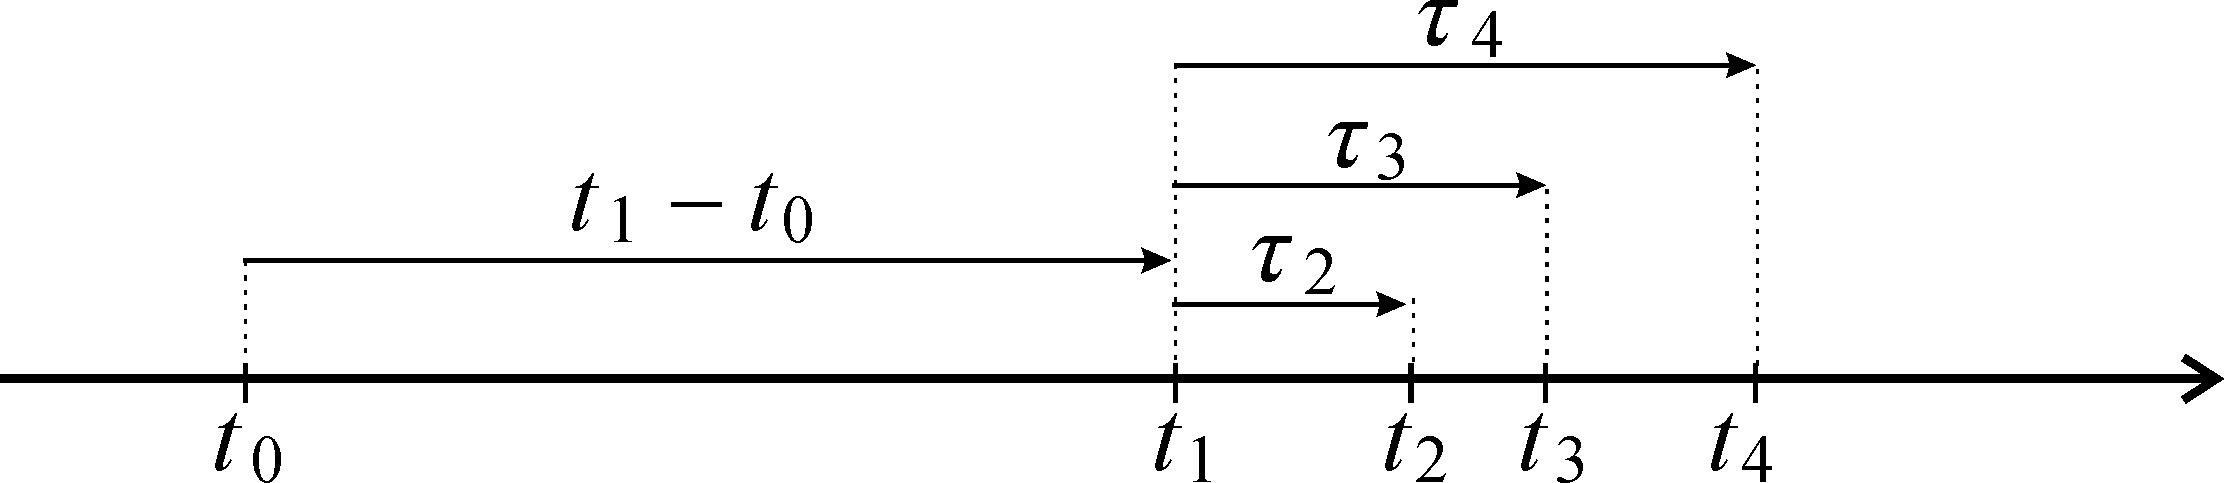
\includegraphics[width=9.5cm]{gps_times} \vspace*{-2mm}
\caption{The emission time $t_{0}$ and the offsets between the arrival times
$\tau_{2},\tau_{3},\tau_{4}$ are known}

\label{fig:gps_times}
\end{figure}


\chapter*{Exercises}

\rule{0.95\columnwidth}{1pt}

\begin{Exercice} \label{ex:loc_triangle} Localization from wall
distance measurements \end{Exercice}

\textcolor{blue}{See the correction video at \href{https://youtu.be/A6dYrlsGl8k}{https://youtu.be/A6dYrlsGl8k}}

\begin{figure}[H]
\centering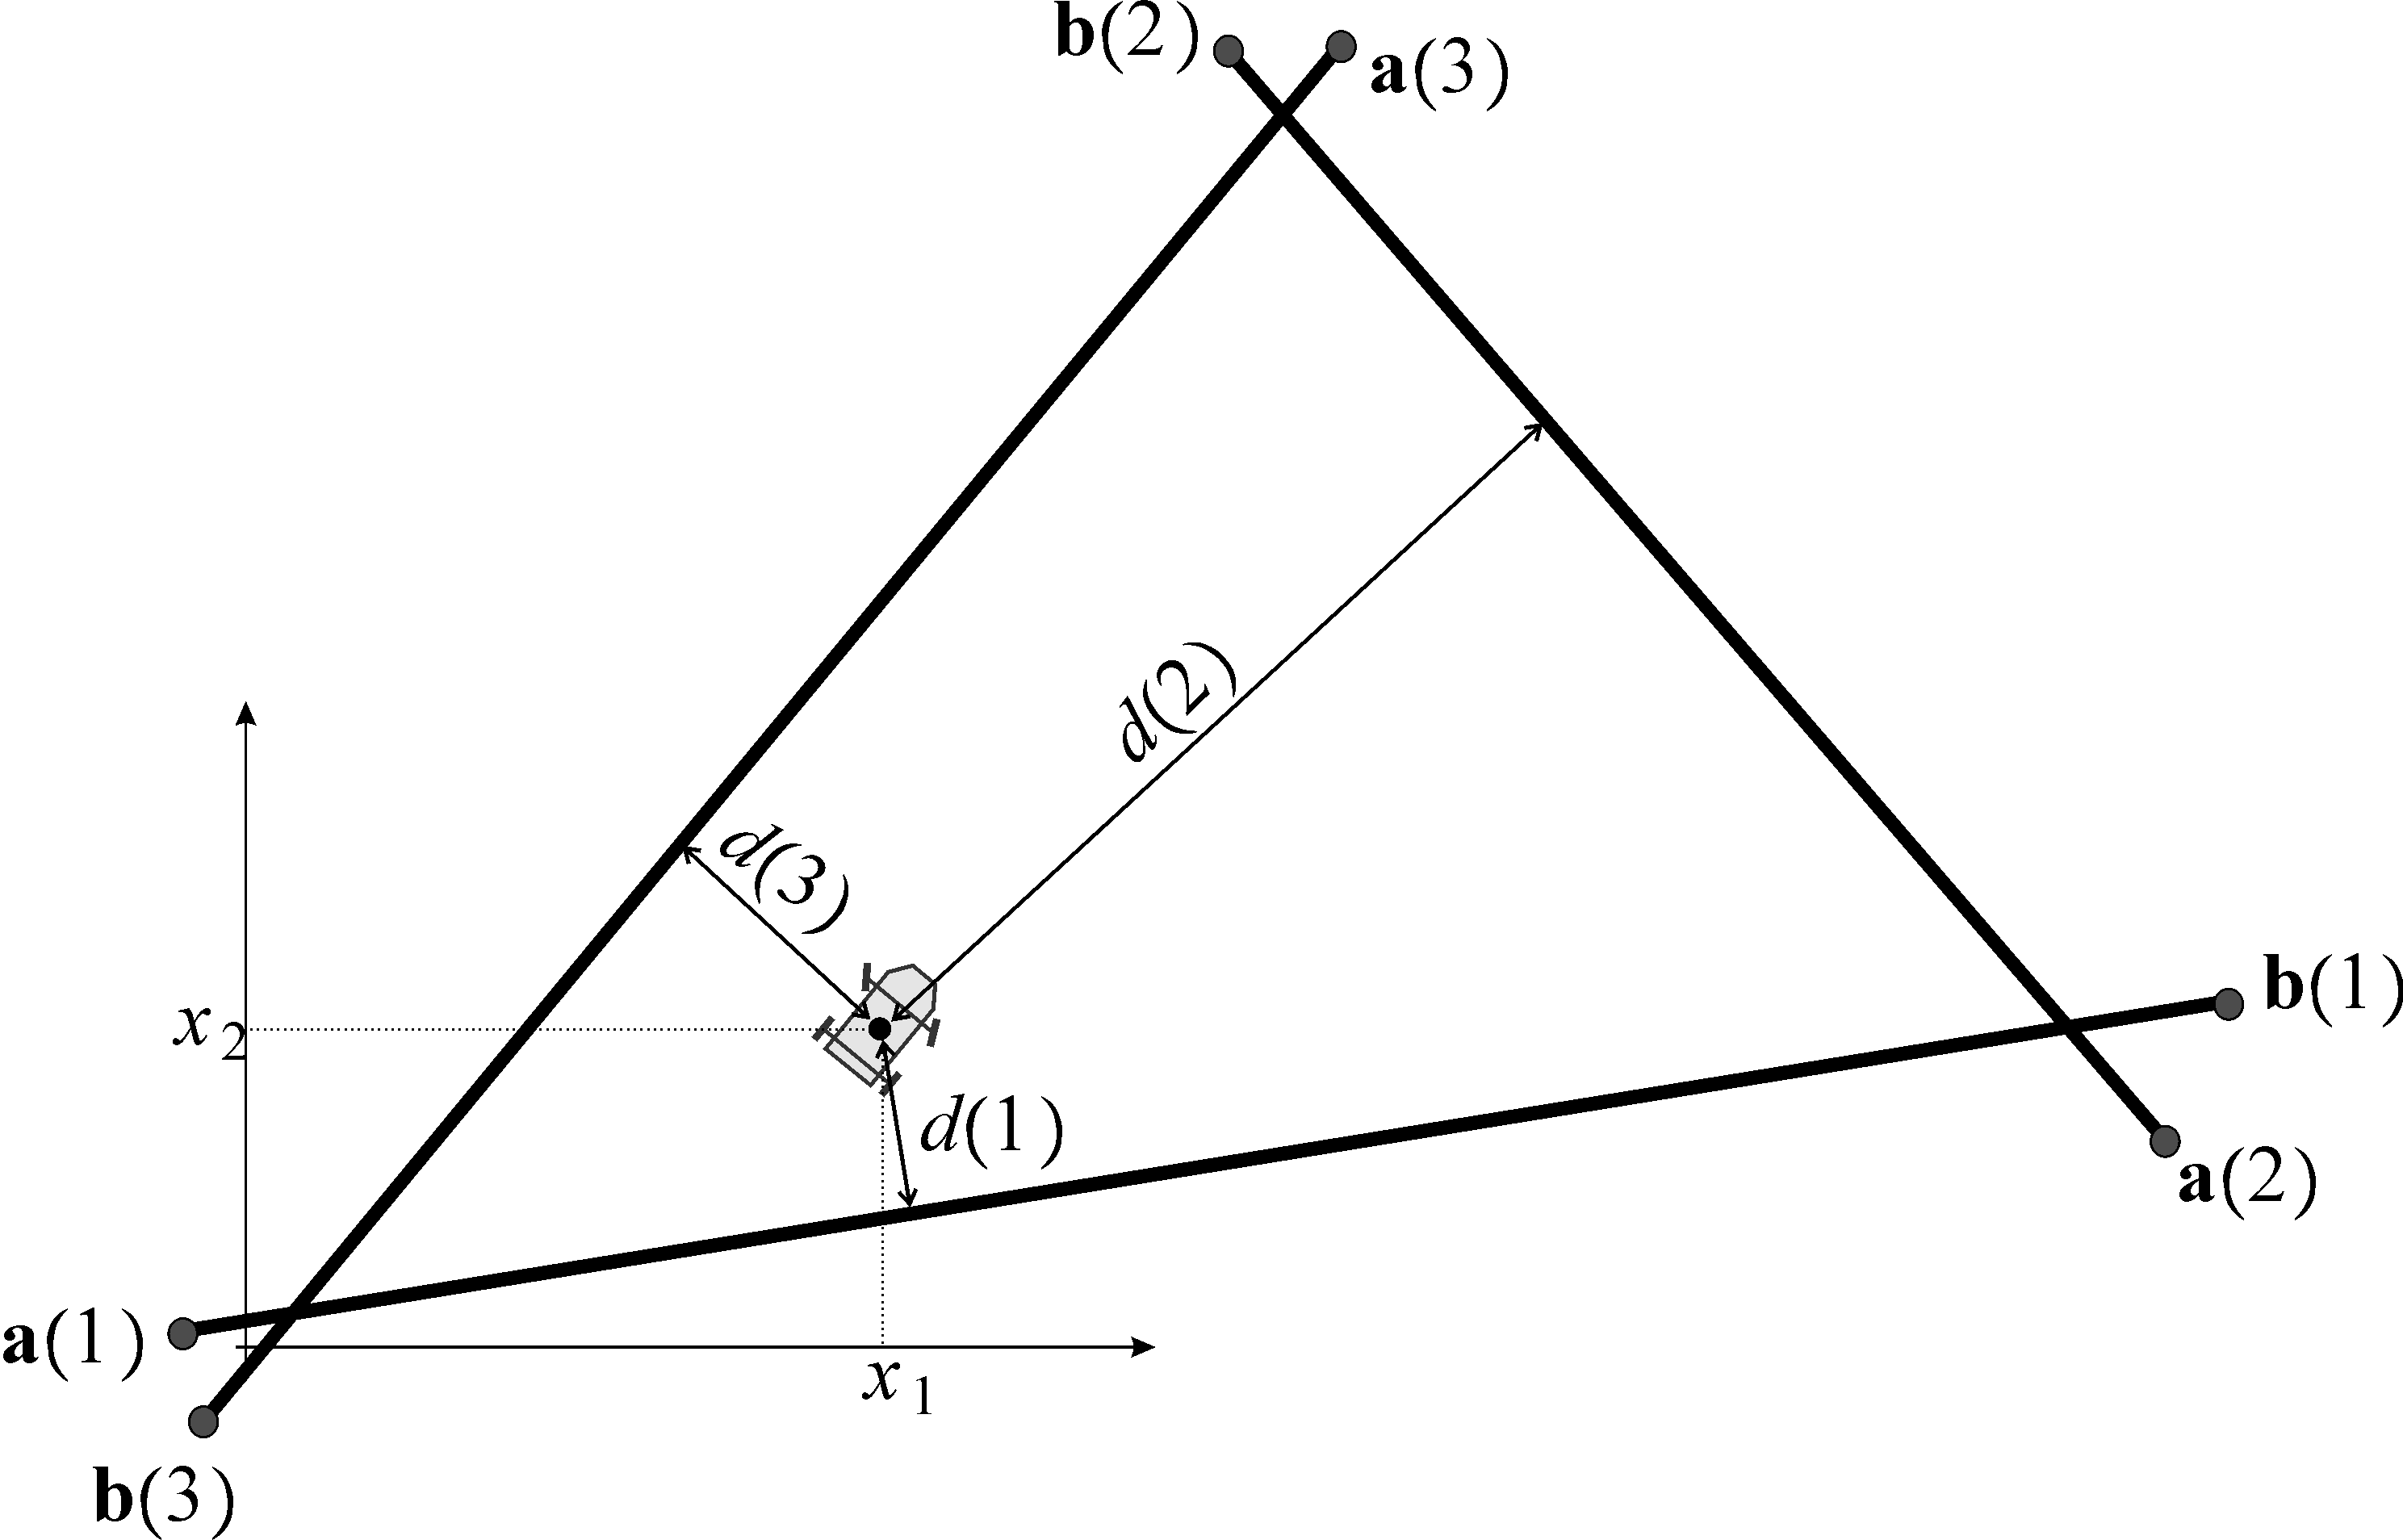
\includegraphics[width=10cm]{kalman_dist}\caption{The robot must locate itself by measuring its distance to the three
walls}

\label{fig:kalman_dist}
\end{figure}

Consider a punctual robot positioned at $\mathbf{x}=\left(x_{1},x_{2}\right)$.
This robot measures its distance to the three walls, as shown in Figure
\ref{fig:kalman_dist}. The $i^{\text{th}}$ wall corresponds to a
line defined by two points $\mathbf{a}\left(i\right)$ and\textbf{\ }$\mathbf{b}\left(i\right)$.
The distance to the $i^{\text{th}}$ wall is: 
\[
d\left(i\right)=\det\left(\mathbf{u}\left(i\right),\mathbf{x}-\mathbf{a}\left(i\right)\right)+\beta_{i}
\]
with $\mathbf{u}\left(i\right)=\frac{\mathbf{b}\left(i\right)-\mathbf{a}\left(i\right)}{\left\Vert \mathbf{b}\left(i\right)-\mathbf{a}\left(i\right)\right\Vert }$.
Each distance is measured with a centered error $\beta_{i}$ with
variance $1$ and all the errors are independent of one other. Before
taking any measurements, the robot assumes it is in position $\mathbf{\bar{x}}=\left(1,2\right)$
with the associated covariance matrix given by $100\cdot\mathbf{I}$
where $\mathbf{I}$ is the identity matrix.

1) Give, in function of the $\mathbf{a}\left(i\right),\mathbf{b}\left(i\right),d\left(i\right)$,
an estimation of the robot's position as well as the covariance matrix
for the error. For this you can use the expression of the unbiased
orthogonal linear estimator or equivalently the expression of the
Kalman filter in correction mode.

2) The coordinates of the points as well as the distances are given
by:
\[
\begin{tabular}{|c|c|c|c|}
\hline  \ensuremath{i}  &  \ensuremath{1}  &  \ensuremath{2}  &  \ensuremath{3}\\
\hline  \ensuremath{\mathbf{a}\left(i\right)}  &  \ensuremath{\left(\begin{array}{c}
2\\
1
\end{array}\right)}  &  \ensuremath{\left(\begin{array}{c}
15\\
5
\end{array}\right)}  &  \ensuremath{\left(\begin{array}{c}
3\\
12
\end{array}\right)}\\
\hline  \ensuremath{\mathbf{b}\left(i\right)}  &  \ensuremath{\left(\begin{array}{c}
15\\
5
\end{array}\right)}  &  \ensuremath{\left(\begin{array}{c}
3\\
12
\end{array}\right)}  &  \ensuremath{\left(\begin{array}{c}
2\\
1
\end{array}\right)}\\
\hline  \ensuremath{d(i)}  &  \ensuremath{2}  &  \ensuremath{5}  &  \ensuremath{4} 
\\\hline \end{tabular}
\]
Write a program that gives us the required estimation.

\rule{0.95\columnwidth}{1pt}

\begin{Exercice} Blind walker\label{exer:kalman:facteur:echelle}
\end{Exercice}

\textcolor{blue}{See the correction video at \href{https://youtu.be/MAkBZiEyt3I}{https://youtu.be/MAkBZiEyt3I}}

We consider a blind walker moving on a horizontal line. Its movement
is described by the discretized state equation: 
\[
\left\{ \begin{array}{lll}
x_{1}\left(k+1\right) & = & x_{1}\left(k\right)+x_{2}\left(k\right)\cdot u\left(k\right)\\
x_{2}\left(k+1\right) & = & x_{2}\left(k\right)+\alpha_{2}\left(k\right)
\end{array}\right.
\]
where $x_{1}\left(k\right)$ is the position of the walker, $x_{2}\left(k\right)$
is the length of a step (referred to as \emph{scale factor}) and $u\left(k\right)$
is the number of steps per time unit. We measure the quantity $u\left(k\right)$.
Thus, at each unit of time, the walker moves a distance of $x_{2}\left(k\right)\cdot u\left(k\right)$.
At the initial moment, we know that $x_{1}$ is zero and that $x_{2}$
is close to $1$. $x_{2}\left(0\right)$ will be represented by a
Gaussian distribution whose mean is equal to $1$ and whose standard
deviation is $0.02$. The scale factor $x_{2}$ evolves slowly by
means of $\alpha_{2}\left(k\right)$ that we will assume to be centered,
white and of standard deviation $0.01.$

1) We apply an input $u\left(k\right)=1$ for $k=0,\dots,9$ and $u\left(k\right)=-1$
for $k=10,\dots,19$. Write a program that implements a predictive
Kalman filter capable of estimating the position $x_{1}\left(k\right)$.

2) Draw the confidence ellipses associated with the probability $\eta=0.99.$
How does the uncertainty evolve for $x_{1}$ in function of $k$ ?

3) Draw the determinant of the covariance matrix $\mathbf{\boldsymbol{\Gamma}}_{\mathbf{x}}$
with respect to $k$. Discuss.

\rule{0.95\columnwidth}{1pt}

\begin{Exercice} \label{ex:kalman:dead:reckoning} Dead reckoning
\end{Exercice}

\textcolor{blue}{See the correction video at \href{https://youtu.be/Zumje1wUOJg}{https://youtu.be/Zumje1wUOJg}}

\emph{Dead reckoning} corresponds to the problem of localization in
which only proprioceptive sensors are available. This type of navigation
was used by early navigators who were trying to locate themselves
during long journeys. They were able to do this in a very approximate
way by measuring the heading of the boat, the speed at various instants
and integrating all the corresponding variations in position over
the entire journey. In a more general context, we may consider that
using a state observer in prediction mode and without correction (in
the particular case in which the state is the position of the robot)
corresponds to dead reckoning. Let us consider the robot represented
on Figure \ref{fig:robot_tricycle} and whose state equations are:
\[
\left(\begin{array}{l}
\dot{x}\\
\dot{y}\\
\dot{\theta}\\
\dot{v}\\
\dot{\delta}
\end{array}\right)=\left(\begin{array}{c}
v\cos\delta\cos\theta\\
v\cos\delta\sin\theta\\
\frac{{\displaystyle v\sin\delta}}{3}+\alpha_{\theta}\\
u_{1}+\alpha_{v}\\
u_{2}+\alpha_{\delta}
\end{array}\right)
\]
where $\alpha_{\theta},\alpha_{v},\alpha_{\delta}$ are independent
continuous-time Gaussian white noises. In a more rigorous way, these
are random distributions with infinite power, but once they are discretized,
the mathematical difficulties disappear.

\begin{figure}[H]
\centering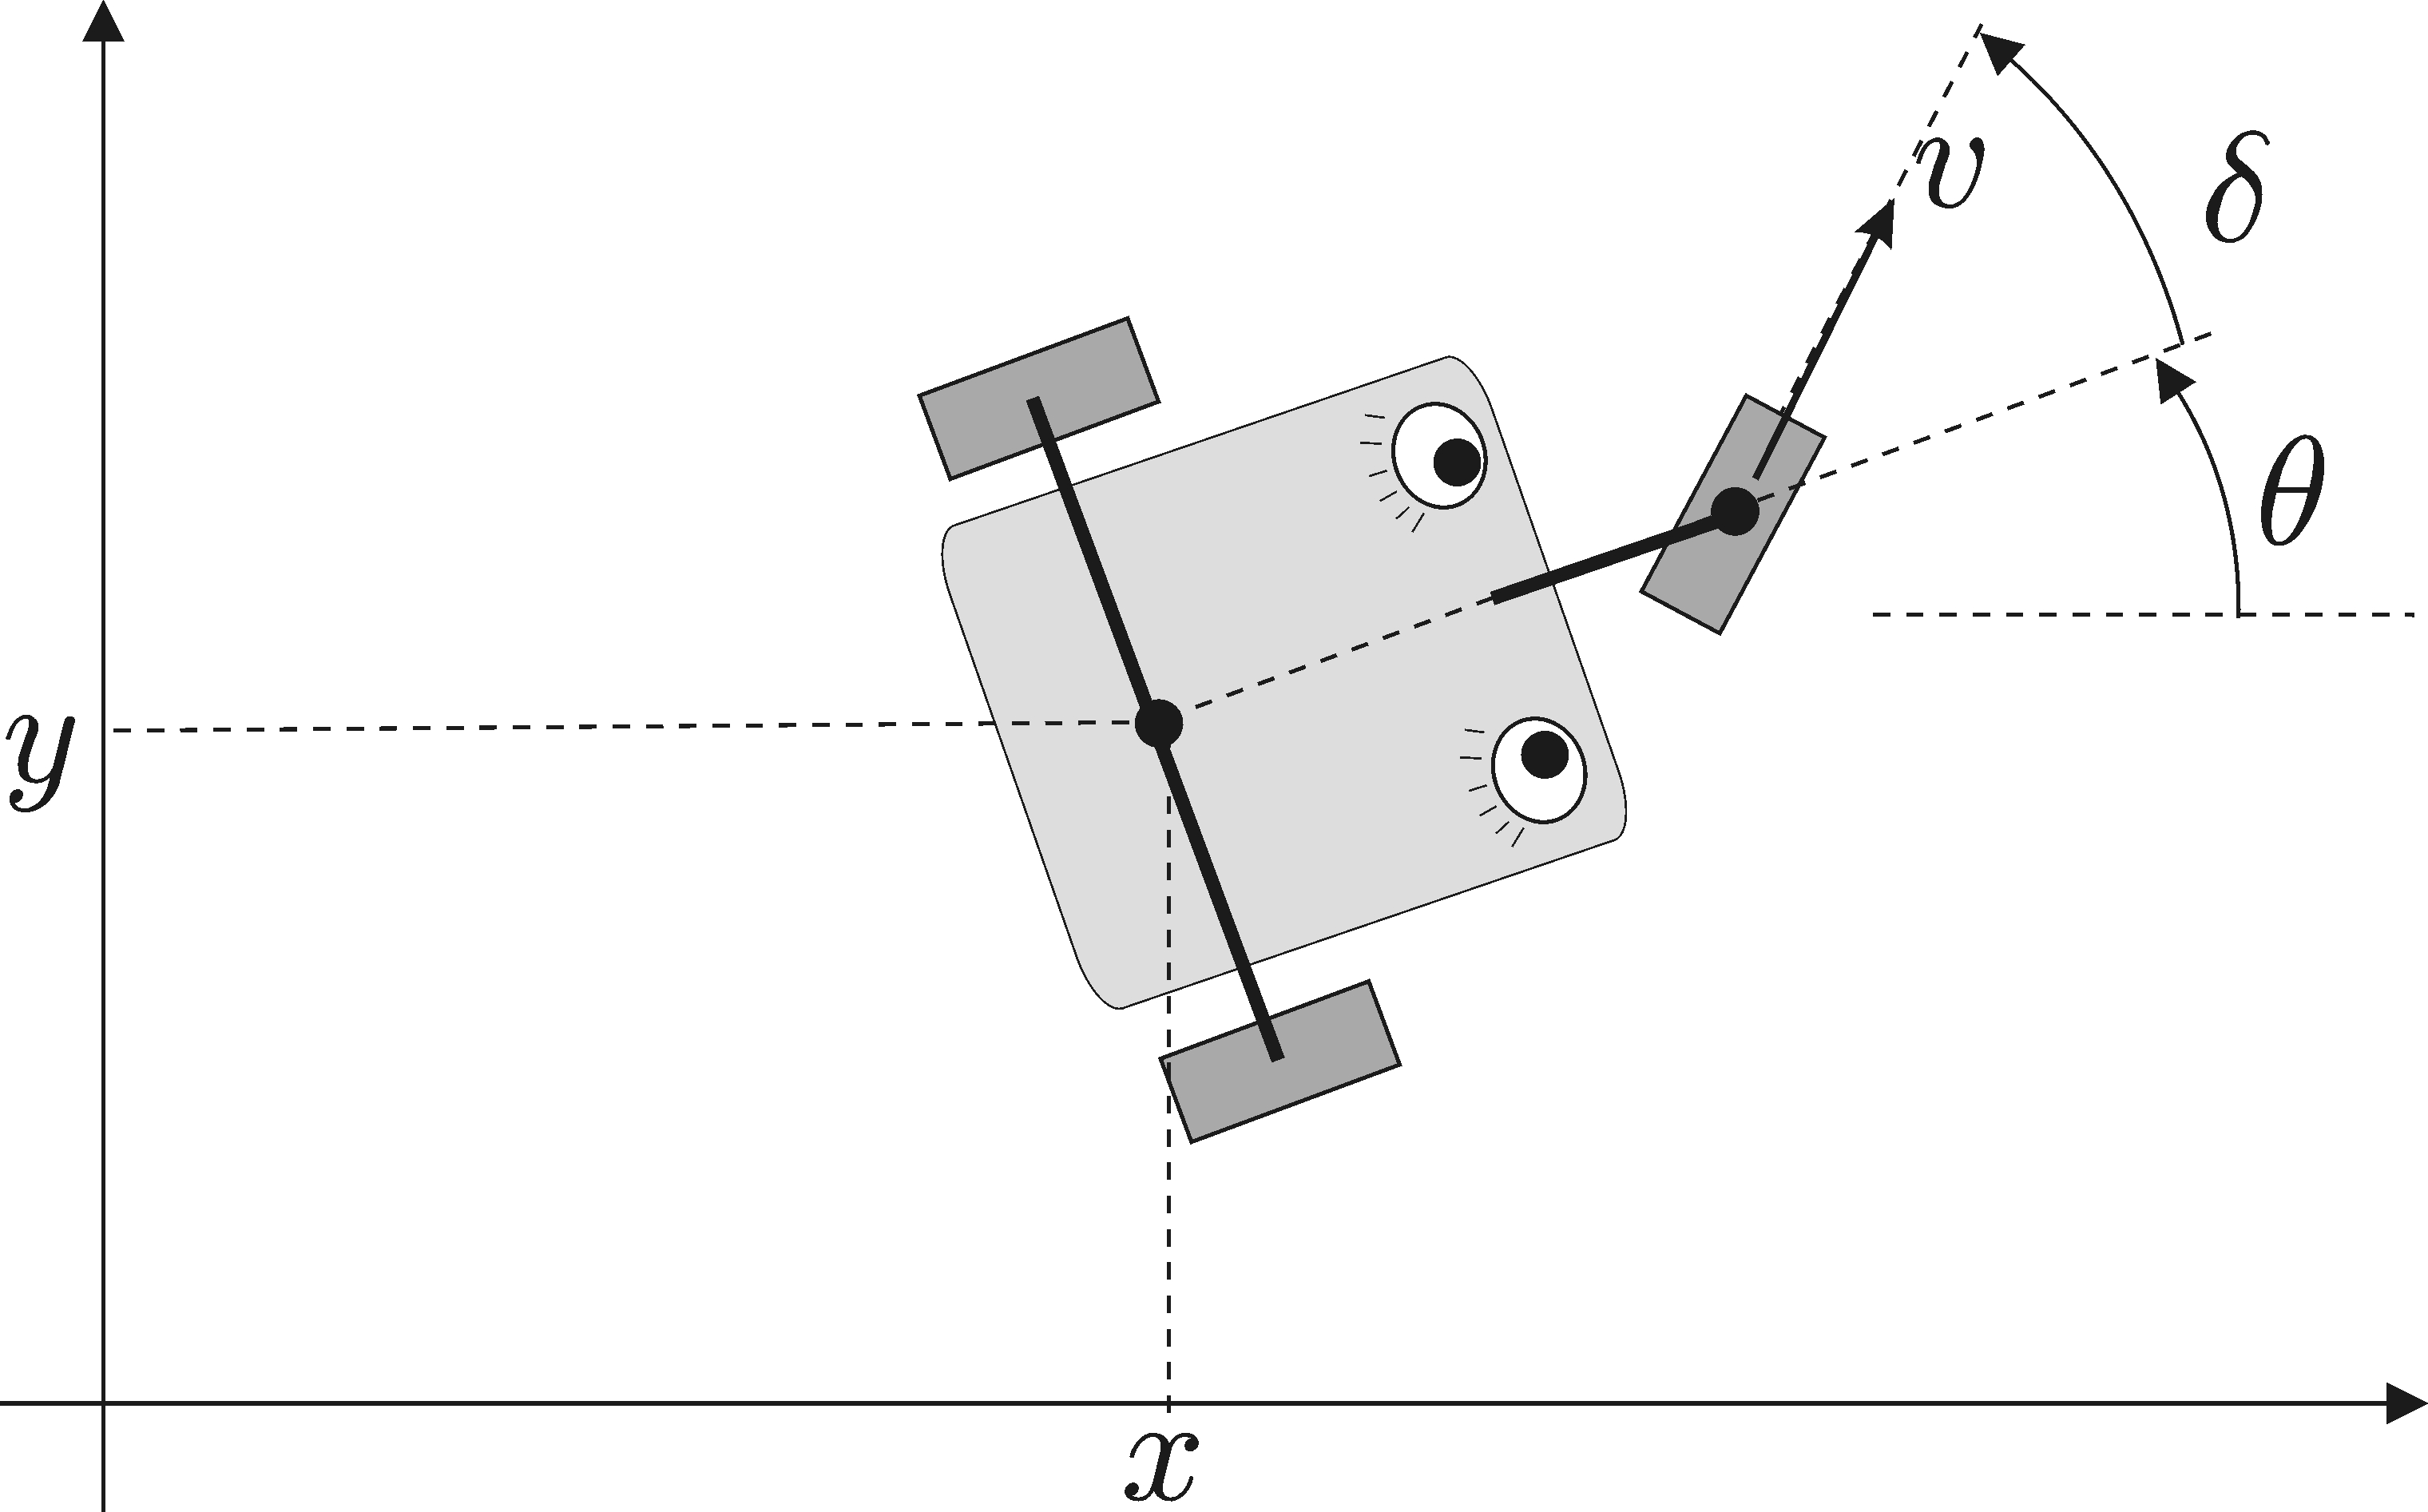
\includegraphics[width=6.368cm,height=3.9803cm]{robot_tricycle}\caption{Dead reckoning for a tricycle robot}

\label{fig:robot_tricycle}
\end{figure}

The robot is equipped with a compass that returns $\theta$ with high
precision and an angle sensor that returns the angle $\delta$ of
the front wheel.

1) Discretize this system with an Euler method. Simulate this system
for an arbitrary input $\mathbf{u}\left(t\right)$ and initial vector.
For the variance of the discretized noises $\alpha_{\theta},\alpha_{v},\alpha_{\delta}$
we will take $0.01\cdot dt$, where $dt$ is the discretization step.

2) Express this localization problem in a linear and discretized form.

3) Using a Kalman filter, predict the position of the robot as well
as the associated covariance matrix.

4) How does the localization program change if we assume that, using
odometers, the robot is capable of measuring its speed $v$ with a
variance of $0.01$ ?

\rule{0.95\columnwidth}{1pt}

\begin{Exercice} \label{ex:localisation:gonio} Goniometric localization$~$
\end{Exercice}

\textcolor{blue}{See the correction video at \href{https://youtu.be/kIhSORI2cwg}{https://youtu.be/kIhSORI2cwg}}

Let u\&s consider once again a robot vehicle described by the state
equations: 
\[
\left(\begin{array}{l}
\dot{x}_{1}\\
\dot{x}_{2}\\
\dot{x}_{3}\\
\dot{x}_{4}\\
\dot{x}_{5}
\end{array}\right)=\left(\begin{array}{c}
x_{4}\cos x_{5}\cos x_{3}\\
x_{4}\cos x_{5}\sin x_{3}\\
\frac{{\displaystyle x_{4}\sin x_{5}}}{3}\\
u_{1}\\
u_{2}
\end{array}\right)
\]
The vector $\left(x_{1},x_{2}\right)$ represents the coordinates
of the center of the robot, $x_{3}$ is the heading of the robot,
$x_{4}$ its speed and $x_{5}$ the angle of its front wheels. The
robot is surrounded by point landmarks $\mathbf{m}(1),\mathbf{m}(2),\dots$
whose positions are known. The robot can only detect these landmarks
$\mathbf{m}(i)$ if the distance to them is sufficiently small (smaller
than $15~$m). In such a case, the robot measures the bearing angle
$\delta_{i}$ with high precision. We will also assume that the robot
knows the angles $x_{3}$ and $x_{5}$ at all times, without any error.
Finally, it measures its speed $x_{4}$ with an error of variance
$1$. Figure \ref{fig:kalman_gonio} illustrates a situation in which
two landmarks $\mathbf{m}(1)$ and $\mathbf{m}(2)$ are detected by
the robot.

\begin{figure}[H]
\centering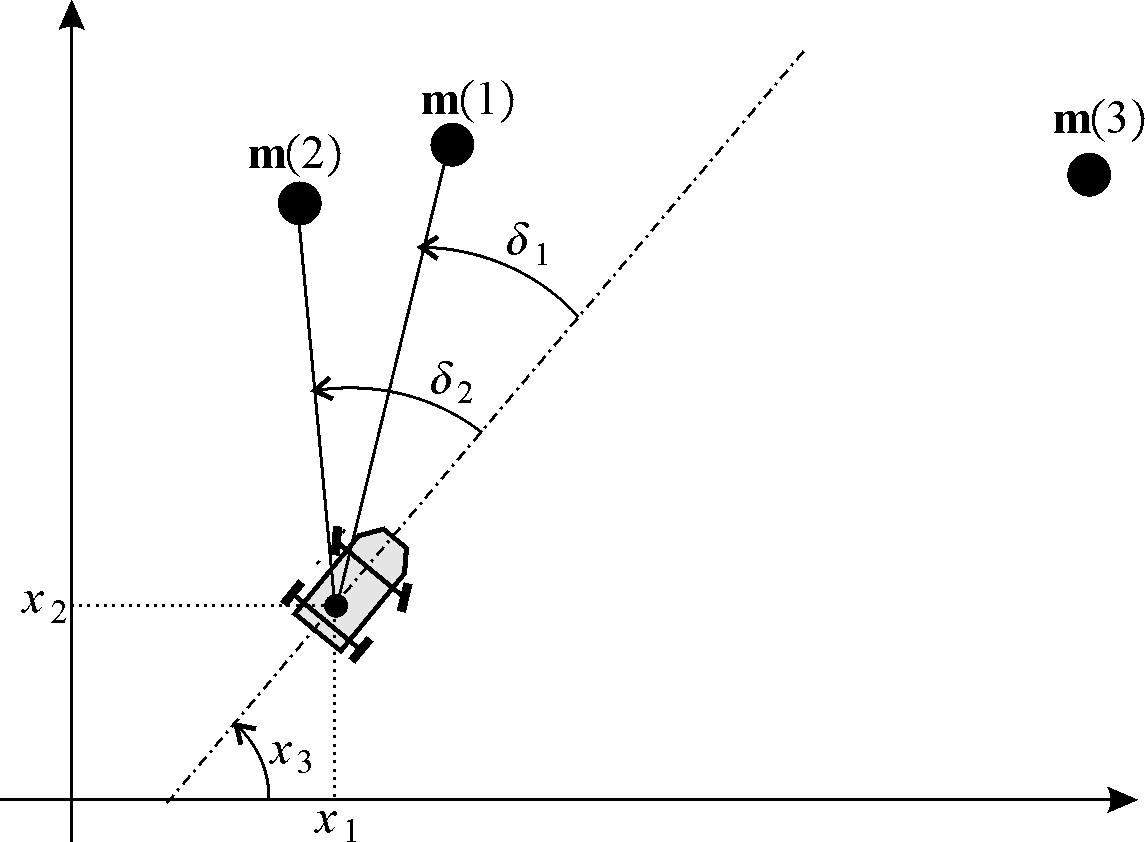
\includegraphics[width=9cm]{kalman_gonio}\caption{Goniometric localization}

\label{fig:kalman_gonio}
\end{figure}

In order for the robot to locate itself, we would like to use a Kalman
filter. For this, we need linear equations, which we do not have here.
Since $x_{3}$ and $x_{5}$ are known, the nonlinearity can be based
on a temporal dependency. Let us take for this $\mathbf{z}=\left(x_{1},x_{2},x_{4}\right)$.

1) Show that $\mathbf{z}$ satisfies a linear state evolution equation.
Find the associated observation equation.

2) Find a discretization for the evolution of $\mathbf{z}$ in order
to feed a Kalman filter.

3) Implement a simulator with the robot surrounded by the following
four landmarks:
\[
\mathbf{a}\left(1\right)=\left(\begin{array}{c}
0\\
25
\end{array}\right),~\mathbf{a}\left(2\right)=\left(\begin{array}{c}
15\\
30
\end{array}\right),~\mathbf{a}\left(3\right)=\left(\begin{array}{c}
30\\
15
\end{array}\right),~\mathbf{a}\left(4\right)=\left(\begin{array}{c}
15\\
20
\end{array}\right)
\]
As stated above, the robot can only goniometrically detect landmarks
once they are close.

4) Implement a Kalman filter for the localization. The initial state
will be assumed unknown.

5) We now have two robots $\mathcal{R}_{a}$ and $\mathcal{R}_{b}$
capable of communicating wirelessly while measuring the landmark angles
(see Figure \ref{fig:kalman_gonio_2robots}). When the distances are
small (i.e. smaller than 20~m), the robots can measure the angles
$\varphi_{a}$ and $\varphi_{b}$ with high precision using cameras
(see figure). Suggest a centralized Kalman filter for the localization
of the two robots.

\begin{figure}[H]
\centering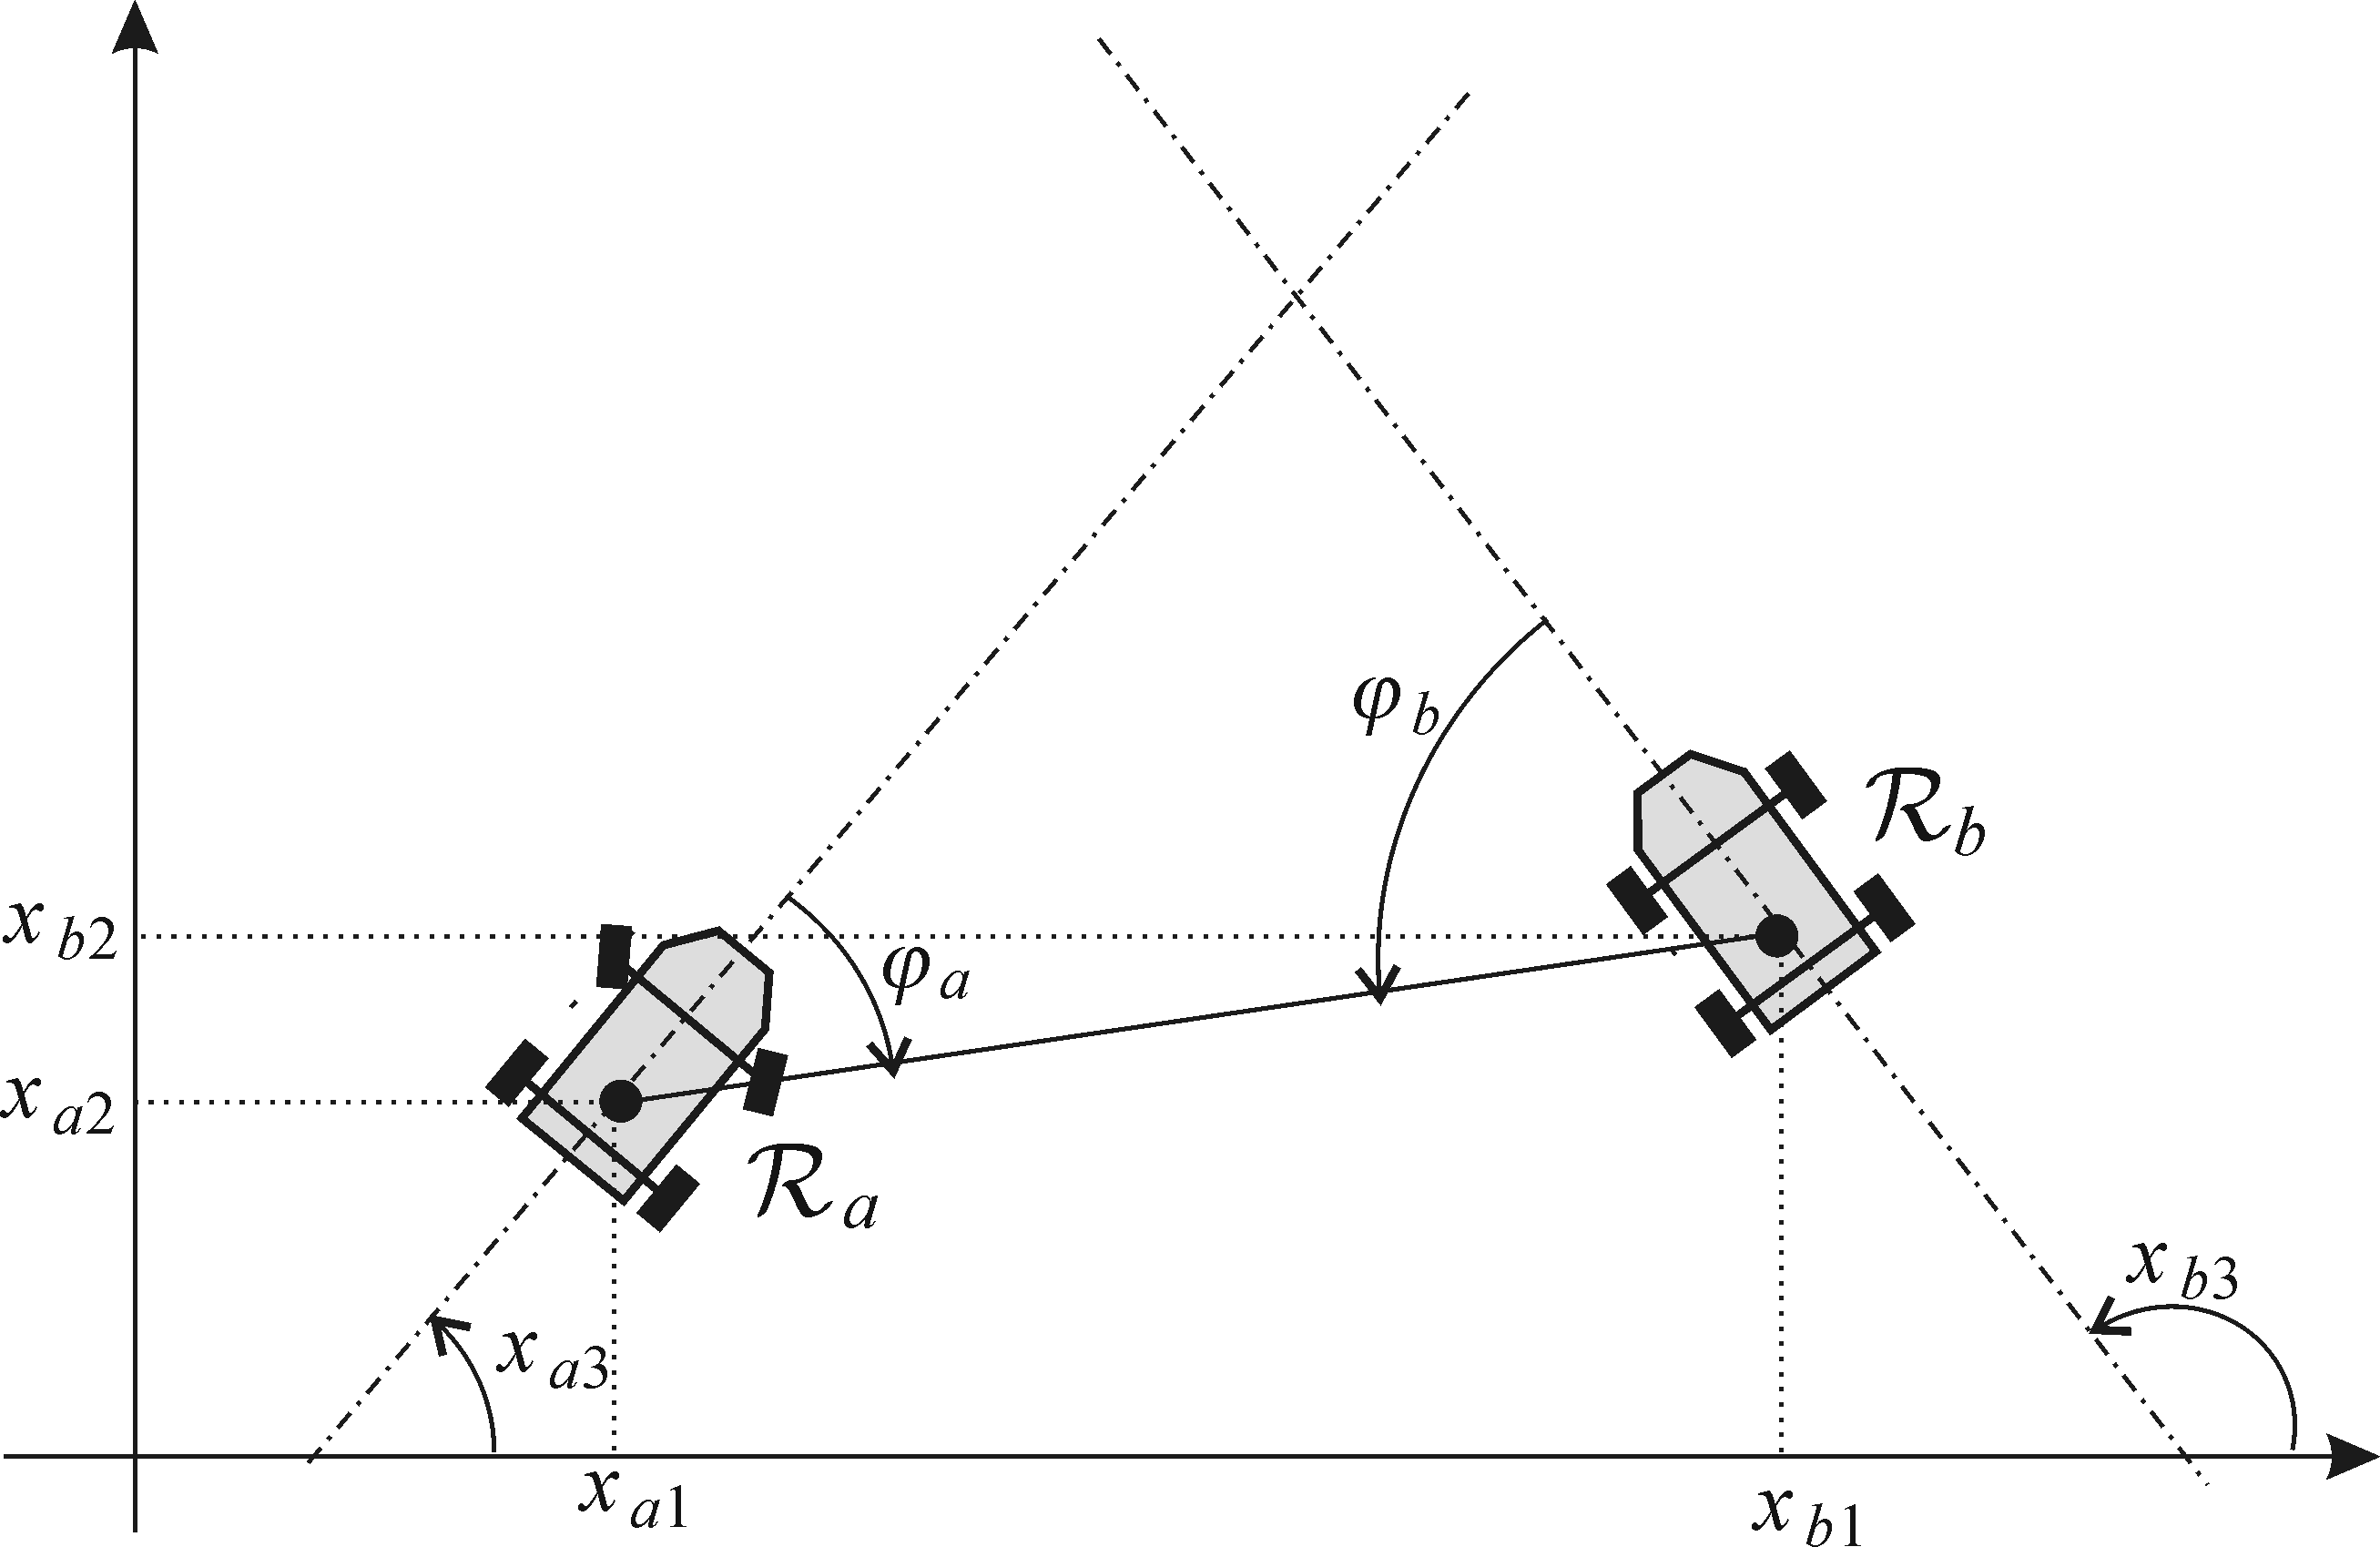
\includegraphics[width=8.5cm]{kalman_gonio_2robots}\caption{Goniometric localization for two communicating robots}

\label{fig:kalman_gonio_2robots}
\end{figure}

\rule{0.95\columnwidth}{1pt}

\begin{Exercice} \label{ex:hokuyo} Localization by lidar \end{Exercice}

\textcolor{blue}{See the correction video at \href{https://youtu.be/V0hOejnwNEo}{https://youtu.be/V0hOejnwNEo}}

Here we are interested in developing a fast and robust localization
method for a robot using a rotating laser rangefinder, or lidar (\emph{light
radar}) of type Hokuyo. The robot has no compass and in located inside
a rectangular room whose length and width are unknown. More precisely,
we want to localize the walls of the rectangular room in the robot
frame.

1) Let $\mathbf{a}_{1},\dots,\mathbf{a}_{n_{p}}$ be points of $\mathbb{R}^{2}$
located on the same line. Find this line using a least squares method.
Represent this line in normal form: 
\[
x\cos\alpha+y\sin\alpha=d\text{, with }d\geq0
\]
where $\alpha,d$ are the parameters of the line.

2) The lidar of the robot has an aperture angle of $180$ degrees.
It returns $n=512$ points $(x_{i},y_{i})$, in the robot frame as
represented by Figure \ref{fig:lidar1}. These points correspond to
real data and can be found in the file \texttt{lidar\_data.csv.} In
the world frame, most of the points, say $70\%$, are supposed to
belong to the rectangle representing our room. 

\begin{figure}[H]
\centering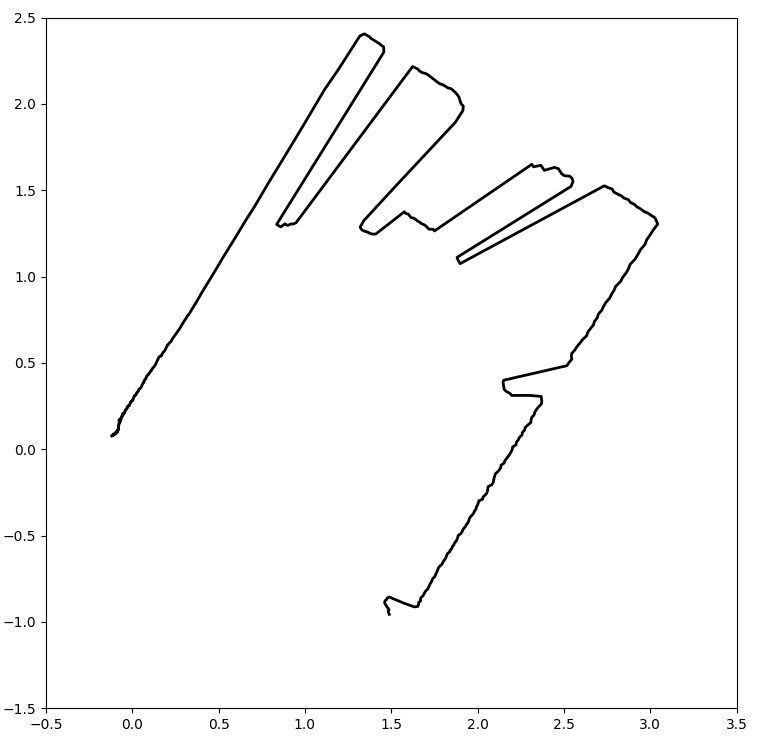
\includegraphics[width=7cm]{lidar1}\caption{Data collected by the lidar}

\label{fig:lidar1}
\end{figure}

Take them in groups of ten (\emph{i.e.}, 51 groups) and try to find
the line that passes the best through each group using the least squares
method. Keep only the groups with a small residue. You should thus
obtain $m$ lines, represented by $m$ points of the form $\left(\beta_{j},d_{j}\right),$
$j\in\left\{ 1,\dots,n\right\} $ in the so-called \emph{Hough space}.
A pair $\left(\beta_{j},d_{j}\right)$ is called an \emph{alignment}.
Write a program which draw all alignments with a small residue.

3) Find the four possible directions for walls of our room (knowing
that it is rectangular). 

4) Associate one wall to each aligment $\left(\beta_{j},d_{j}\right)$.

5) Write a program which localizes the walls of the room in the robot
frame from the data set given in the file \texttt{lidar\_data}.csv.

\rule{0.95\columnwidth}{1pt}


\chapter{Observers}

\section{Kalman-Bucy\label{sec:Kalman-Bucy}}

We now consider the linear continuous time system described by
\[
\left\{ \begin{array}{lll}
\mathbf{\dot{x}}_{t} & = & \mathbf{A}_{t}\mathbf{x}_{t}+\mathbf{u}_{t}+\boldsymbol{\alpha}_{t}\\
\mathbf{y}_{t} & = & \mathbf{C}_{t}\mathbf{x}_{t}+\boldsymbol{\beta}_{t}
\end{array}\right.
\]
where $\mathbf{u}_{t}$ and $\mathbf{y}_{t}$ are known for all $t$.
The noise $\boldsymbol{\alpha}_{t}$ and $\boldsymbol{\beta}_{t}$
are assumed to be white and Gaussian. For a better understanding,
the order of the quantities that will be used with respect to $dt$
(assumed to be infinitely small) are recalled below

\begin{tabular}{|c|c|c|c|}
\hline 
Size & Order & Random & Deterministic\tabularnewline
\hline 
\hline 
Infinitely small & $O\left(dt\right)$ & $\boldsymbol{\alpha}_{k}$ & $\mathbf{K}_{t}$,$\mathbf{u}_{k}$\tabularnewline
\hline 
Medium & $O\left(1\right)$ & $\mathbf{x}_{t},\mathbf{x}_{k}$ & $\mathbf{\boldsymbol{\Gamma}}_{\boldsymbol{\alpha}},\mathbf{\boldsymbol{\Gamma}}_{\boldsymbol{\beta}},\mathbf{K}_{b},\mathbf{u}_{t},\mathbf{A}_{t},\mathbf{C}_{t}$\tabularnewline
\hline 
Infinitely Large & $O\left(\frac{1}{dt}\right)$ & $\boldsymbol{\alpha}_{t},\boldsymbol{\beta}_{t},\boldsymbol{\beta}_{k},\mathbf{\dot{x}}_{t},\mathbf{y}_{t}$ & $\boldsymbol{\Gamma}_{\boldsymbol{\alpha}_{t}},\boldsymbol{\Gamma}_{\boldsymbol{\beta}_{t}}$\tabularnewline
\hline 
\end{tabular}

The covariance matrices $\boldsymbol{\Gamma}_{\boldsymbol{\alpha}_{t}}$,$\boldsymbol{\Gamma}_{\boldsymbol{\beta}_{t}}$
for $\mathbf{\boldsymbol{\alpha}}_{t}$ et $\mathbf{\boldsymbol{\beta}}_{t}$
and are infinite ($O\left(\frac{1}{dt}\right)$) and we write $\boldsymbol{\Gamma}_{\boldsymbol{\alpha}_{t}}=\frac{1}{dt}\cdot\boldsymbol{\Gamma}_{\mathbf{\boldsymbol{\alpha}}}$
and $\boldsymbol{\Gamma}_{\boldsymbol{\beta}_{t}}=\frac{1}{dt}\cdot\boldsymbol{\Gamma}_{\mathbf{\boldsymbol{\beta}}}$. 

\textbf{Remark}. The fact that $\mathbf{\dot{x}}_{t},\mathbf{y}_{t}$
are considered as infinite, due to the fact the noises $\boldsymbol{\alpha}_{t},\boldsymbol{\beta}_{t}$
are also infinite. If all would have been finite, the state could
have been found in a infinitely small time. To be able to deal properly
with these infinitely large quantities, distribution theory is needed.
Here, we will not use these difficult notions and consider classical
notions from signal processing. Note that this type of simplification
is usually made in physics, as for instance when we assimilate the
Dirac distribution to the Dirac function $\delta_{0}\left(t\right).$

Since we have
\[
\begin{array}{cll}
\mathbf{x}_{t+dt} & = & \mathbf{x}_{t}+\int_{t}^{t+dt}\mathbf{\dot{x}}_{\tau}d\tau\\
 & = & \mathbf{x}_{t}+\int_{t}^{t+dt}\left(\mathbf{A}_{\tau}\mathbf{x}_{\tau}+\mathbf{u}_{\tau}+\boldsymbol{\alpha}_{\tau}\right)d\tau\\
 &  & \mathbf{x}_{t}+dt\cdot\left(\mathbf{A}_{t}\mathbf{x}_{t}+\mathbf{u}_{t}\right)+\int_{t}^{t+dt}\boldsymbol{\alpha}_{\tau}d\tau
\end{array}
\]
a discretization with a sampling time $dt$ is 
\[
\left\{ \begin{array}{cccl}
\underset{\mathbf{x}_{k+1}}{\underbrace{\mathbf{x}_{t+dt}}} & = & \underset{\mathbf{A}_{k}}{\underbrace{\left(\mathbf{I}+dt\cdot\mathbf{A}_{t}\right)}}\cdot\underset{\mathbf{x}_{k}}{\underbrace{\mathbf{x}_{t}}} & +\underset{\mathbf{u}_{k}}{\underbrace{dt\cdot\mathbf{u}_{t}}}+\underset{\boldsymbol{\alpha}_{k}}{\underbrace{\int_{t}^{t+dt}\boldsymbol{\alpha}_{\tau}d\tau}}\\
\underset{\mathbf{y}_{k}}{\underbrace{\mathbf{y}_{t}}} & = & \underset{\mathbf{C}_{k}}{\underbrace{\mathbf{C}_{t}}}\cdot\underset{\mathbf{x}_{k}}{\underbrace{\mathbf{x}_{t}}} & +\underset{\boldsymbol{\beta}_{k}}{\underbrace{\boldsymbol{\beta}_{t}}}.
\end{array}\right.
\]
Note that, as explained in Exercise \ref{ex:brownien}, the covariance
for the state noise $\boldsymbol{\alpha}_{k}$ increases linearly
with $dt$. More precisely, 
\[
\boldsymbol{\Gamma}_{\boldsymbol{\alpha}_{k}}=dt\cdot\mathbf{\boldsymbol{\Gamma}}_{\mathbf{\boldsymbol{\alpha}}}.
\]
This means that when $dt$ is infinitely small, $\boldsymbol{\alpha}_{k}$
is infinitely small, whereas $\boldsymbol{\alpha}_{t}$ is infinitely
large (otherwise $\boldsymbol{\alpha}_{k}$ would be equal to zero).
The measurement $\mathbf{y}_{k}$ represents a fusion of all measurement
$\mathbf{y}_{t}$ with $t\in[t,t+dt]$. As for $\boldsymbol{\beta}_{t}$,
its covariance matrix is 
\[
\mathbf{\boldsymbol{\Gamma}}_{\boldsymbol{\beta}_{k}}=\frac{1}{dt}\cdot\mathbf{\boldsymbol{\Gamma}}_{\mathbf{\boldsymbol{\beta}}}.
\]
We now have a linear discrete-time system, and we can apply the classical
Kalman filter given at Section \ref{sec:Kalman-filter}. We have the
following correspondences.

\[
\begin{array}{ccccccccccc}
\mathbf{A}_{k} & \rightarrow & \left(\mathbf{I}+dt\mathbf{A}_{t}\right) &  & \mathbf{u}_{k} & \rightarrow & dt\cdot\mathbf{u}_{t} &  & \boldsymbol{\alpha}_{k} & \rightarrow & \int_{t}^{t+dt}\mathbf{\boldsymbol{\alpha}}_{\tau}d\tau\\
\mathbf{\hat{x}}_{k+1|k} & \rightarrow & \mathbf{\hat{x}}_{t+dt} & \,\,\,\,\, & \mathbf{\hat{x}}_{k|k-1} & \rightarrow & \mathbf{\hat{x}}_{t} & \,\,\,\,\, & \mathbf{\hat{x}}_{k|k} & \rightarrow & \mathbf{\mathring{x}}_{t}\\
\boldsymbol{\Gamma}_{k+1|k} & \rightarrow & \boldsymbol{\Gamma}_{t+dt} &  & \boldsymbol{\Gamma}_{k|k-1} & \rightarrow & \boldsymbol{\Gamma}_{t} &  & \boldsymbol{\Gamma}_{k|k} & \rightarrow & \boldsymbol{\mathring{\Gamma}}_{t}\\
\boldsymbol{\Gamma}_{\boldsymbol{\alpha}_{k}} & \rightarrow & dt\cdot\boldsymbol{\Gamma}_{\boldsymbol{\alpha}} &  & \boldsymbol{\Gamma}_{\boldsymbol{\beta}_{k}} & \rightarrow & \frac{1}{dt}\cdot\boldsymbol{\Gamma}_{\mathbf{\boldsymbol{\beta}}}
\end{array}\,
\]
 The Kalman filter becomes

\[
\left\{ \begin{array}{lll}
\mathbf{\hat{x}}_{t+dt} & = & (\mathbf{I}+dt\mathbf{A}_{t}){\color{red}\mathbf{\mathring{x}}_{t}}+dt\cdot\mathbf{u}_{t}\\
\mathbf{\mathbf{\boldsymbol{\Gamma}}}_{t+dt} & = & (\mathbf{I}+dt\mathbf{A}_{t})\cdot{\color{blue}\mathbf{\boldsymbol{\mathring{\Gamma}}}}_{{\color{blue}t}}\cdot(\mathbf{I}+dt\mathbf{A}_{t})^{T}+dt\boldsymbol{\Gamma}_{\boldsymbol{\alpha}}\\
{\color{red}\mathbf{\mathring{x}}_{t}} & {\color{red}=} & {\color{red}\mathbf{\hat{x}}_{t}\mathbf{+K}_{t}\cdot\widetilde{\mathbf{y}}_{t}}\\
{\color{blue}\mathbf{\boldsymbol{\mathring{\Gamma}}}_{t}} & = & {\color{blue}(\mathbf{\mathbf{I}}-\mathbf{K}_{t}\mathbf{C}_{t})\cdot\mathbf{\mathbf{\boldsymbol{\Gamma}}}_{t}}\\
{\color{red}\widetilde{\mathbf{y}}_{t}} & {\color{red}=} & {\color{red}\mathbf{y}_{t}-\mathbf{C}_{t}\mathbf{\hat{x}}_{t}}\\
\mathbf{S}_{t} & = & {\color{magenta}\mathbf{C}_{t}\mathbf{\mathbf{\boldsymbol{\Gamma}}}_{t}\mathbf{C}_{t}^{\text{T}}}+\frac{1}{dt}\cdot\boldsymbol{\Gamma}_{\mathbf{\boldsymbol{\beta}}}\\
\mathbf{K}_{t} & = & \mathbf{\mathbf{\boldsymbol{\Gamma}}}_{t}\mathbf{C}_{t}^{\text{T}}\mathbf{S}_{t}^{-1}
\end{array}\right.
\]
Taking into account the fact that ${\color{magenta}\mathbf{C}_{t}\mathbf{\mathbf{\boldsymbol{\Gamma}}}_{t}\mathbf{C}_{t}^{\text{T}}}$
is small (line (vi)) compared to $\frac{1}{dt}\cdot\mathbf{\boldsymbol{\Gamma}}_{\mathbf{\boldsymbol{\beta}}}$
(which is infinitely large) and we can simplify it, i.e., $\mathbf{S}_{t}=\frac{1}{dt}\cdot\boldsymbol{\Gamma}_{\mathbf{\boldsymbol{\beta}}}\left(t\right)$,
We conclude that $\mathbf{S}_{t}$ is huge ($=O(1/dt)$) and thus
that $\mathbf{S}_{t}^{-1}$ at line (viii) is small ($=O(dt)$). The
Kalman filter becomes
\[
\left\{ \begin{array}{lll}
\mathbf{\hat{x}}_{t+dt} & = & \left(\mathbf{I}+dt\mathbf{A}_{t}\right)\left({\color{red}\mathbf{\hat{x}}_{t}\mathbf{+K}_{t}\cdot\left(\mathbf{y}_{t}-\mathbf{C}_{t}\mathbf{\hat{x}}_{t}\right)}\right)+dt\cdot\mathbf{u}_{t}\\
\mathbf{\mathbf{\boldsymbol{\Gamma}}}_{t+dt} & = & \left(\mathbf{I}+dt\mathbf{A}_{t}\right)\cdot{\color{blue}\left(\mathbf{\mathbf{I}}-\mathbf{K}_{t}\mathbf{C}_{t}\right)\mathbf{\mathbf{\boldsymbol{\Gamma}}}_{t}}\cdot\left(\mathbf{I}+dt\mathbf{A}_{t}\right)^{T}+dt\boldsymbol{\Gamma}_{\boldsymbol{\alpha}}\\
\mathbf{K}_{t} & = & dt\mathbf{\mathbf{\boldsymbol{\Gamma}}}_{t}\mathbf{C}_{t}^{\text{T}}\boldsymbol{\Gamma}_{\mathbf{\boldsymbol{\beta}}}^{-1}.
\end{array}\right.
\]
Since $\mathbf{K}_{t}$ is small ($=O(dt)$), it is more convenient
to introduce the \emph{Kalman-Bucy} \index{Kalman-Bucy} gain given
by $\mathbf{K}_{b}=\mathbf{\mathbf{\boldsymbol{\Gamma}}}_{t}\mathbf{C}_{t}^{\text{T}}\mathbf{\boldsymbol{\Gamma}}_{\mathbf{\boldsymbol{\beta}}}^{-1}$
which is $O(1)$, \emph{i.e.}, neither infinitely small nor infinitely
large. We have
\[
\left\{ \begin{array}{lll}
\mathbf{\hat{x}}_{t+dt} & = & \underset{=\left(\mathbf{I}+dt\mathbf{A}_{t}\right)\mathbf{\hat{x}}_{t}+dt\mathbf{K}_{b}\cdot\left(\mathbf{y}_{t}-\mathbf{C}_{t}\mathbf{\hat{x}}_{t}\right)+O\left(dt\right)^{2}}{\underbrace{\left(\mathbf{I}+dt\mathbf{A}_{t}\right)\left({\color{red}\mathbf{\hat{x}}_{t}+dt\mathbf{K}_{b}\cdot\left(\mathbf{y}_{t}-\mathbf{C}_{t}\mathbf{\hat{x}}_{t}\right)}\right)}}+dt\cdot\mathbf{u}_{t}\\
\mathbf{\mathbf{\boldsymbol{\Gamma}}}_{t+dt} & = & \underset{=\mathbf{\mathbf{\boldsymbol{\Gamma}}}_{t}+dt\left(\mathbf{A}_{t}\mathbf{\mathbf{\boldsymbol{\Gamma}}}_{t}-\mathbf{K}_{b}\mathbf{C}_{t}\mathbf{\mathbf{\boldsymbol{\Gamma}}}_{t}+\mathbf{\mathbf{\boldsymbol{\Gamma}}}_{t}\mathbf{A}_{t}^{T}\right)+O\left(dt\right)^{2}}{\underbrace{\left(\mathbf{I}+dt\mathbf{A}_{t}\right)\cdot{\color{blue}\left(\mathbf{\mathbf{I}}-dt\mathbf{K}_{b}\mathbf{C}_{t}\right)\mathbf{\mathbf{\boldsymbol{\Gamma}}}_{t}}\cdot\left(\mathbf{I}+dt\mathbf{A}_{t}\right)^{T}}}+dt\boldsymbol{\Gamma}_{\boldsymbol{\alpha}}\\
\mathbf{K}_{b} & = & \mathbf{\mathbf{\boldsymbol{\Gamma}}}_{t}\mathbf{C}_{t}^{\text{T}}\boldsymbol{\Gamma}_{\mathbf{\boldsymbol{\beta}}}^{-1}
\end{array}\right.
\]
Or equivalently
\[
\left\{ \begin{array}{lll}
\frac{\mathbf{\hat{x}}_{t+dt}-\mathbf{\hat{x}}_{t}}{dt} & = & \mathbf{A}_{t}\mathbf{\hat{x}}_{t}+\mathbf{K}_{b}\cdot\left(\mathbf{y}_{t}-\mathbf{C}_{t}\mathbf{\hat{x}}_{t}\right)+\mathbf{u}_{t}\\
\frac{\boldsymbol{\Gamma}_{t+dt}-\boldsymbol{\Gamma}_{t}}{dt} & = & \left(\mathbf{A}_{t}\boldsymbol{\Gamma}_{t}-\mathbf{K}_{b}{\color{blue}\mathbf{C}_{t}\boldsymbol{\Gamma}_{t}}+\mathbf{\mathbf{\boldsymbol{\Gamma}}}_{t}\mathbf{A}_{t}^{\textnormal{T}}\right)+\boldsymbol{\Gamma}_{\boldsymbol{\alpha}}\\
\mathbf{K}_{b} & = & \boldsymbol{\Gamma}_{t}\mathbf{C}_{t}^{\text{T}}\boldsymbol{\Gamma}_{\mathbf{\boldsymbol{\beta}}}^{-1}.
\end{array}\right.
\]
Now, $\,{\color{blue}\mathbf{C}_{t}\boldsymbol{\Gamma}_{t}}=\left(\mathbf{\boldsymbol{\Gamma}}_{t}\mathbf{C}_{t}^{\text{T}}\right)^{T}=\left(\mathbf{K}_{b}\boldsymbol{\Gamma}_{\mathbf{\boldsymbol{\beta}}}\right)^{T}=\mathbf{\boldsymbol{\Gamma}}_{\boldsymbol{\beta}}\mathbf{K}_{b}^{\textnormal{T}}$.
Therefore, we get the Kalman-Bucy filter: 
\[
\left\{ \begin{array}{lll}
\frac{d}{dt}\mathbf{\hat{x}}_{t} & = & \mathbf{A}_{t}\mathbf{\hat{x}}_{t}+\mathbf{K}_{b}\left(\mathbf{y}_{t}-\mathbf{C}_{t}\mathbf{\hat{x}}_{t}\right)+\mathbf{u}_{t}\\
\frac{d}{dt}\mathbf{\mathbf{\boldsymbol{\Gamma}}}_{t} & = & \mathbf{A}_{t}\mathbf{\mathbf{\boldsymbol{\Gamma}}}_{t}+\mathbf{\mathbf{\boldsymbol{\Gamma}}}_{t}\cdot\mathbf{A}_{t}^{\textnormal{T}}-\mathbf{K}_{b}{\color{blue}\mathbf{\boldsymbol{\Gamma}}_{\boldsymbol{\beta}}\mathbf{K}_{b}^{T}}+\boldsymbol{\Gamma}_{\boldsymbol{\alpha}}\\
\mathbf{K}_{b} & = & \mathbf{\mathbf{\boldsymbol{\Gamma}}}_{t}\mathbf{C}_{t}^{\text{T}}\boldsymbol{\Gamma}_{\mathbf{\boldsymbol{\beta}}}^{-1}.
\end{array}\right.
\]
The advantage of the latter formulation compared to the former is
that the product $\mathbf{K}_{b}{\color{blue}\mathbf{\boldsymbol{\Gamma}}_{\boldsymbol{\beta}}\mathbf{K}_{b}^{T}}$
is more stable than $\mathbf{K}_{b}{\color{blue}\mathbf{C}_{t}\boldsymbol{\Gamma}_{t}}$,
since it preserves the symmetry of the resulting matrix. This Kalman-Bucy
filter corresponds to a continuous version of the Kalman filter. In
its formulation all quantities that are $O\left(1\right)$ and thus
no more infinitely small ($O(dt)$) or infinitely large ($O\left(\frac{1}{dt}\right)$)
quantities appear.

\textbf{Remark}. The Kalman-Bucy allows us to understand some effects
that occur when the discrete-time Kalman filter is used for continuous
time systems, such as a robot described by
\[
\left\{ \begin{array}{lll}
\mathbf{\dot{x}} & = & \mathbf{f}_{c}(\mathbf{x},\mathbf{u})\\
\mathbf{y} & = & \mathbf{g}(\mathbf{x})
\end{array}\right.
\]
To perform a simulation, we discretize it, for instance using an Euler
integration. We get
\[
\left\{ \begin{array}{ll}
\mathbf{x}_{k+1} & =\mathbf{f}(\mathbf{x}_{k},\mathbf{u}_{k})+\text{\ensuremath{\boldsymbol{\alpha}}}_{k}\\
\mathbf{y}_{k} & =\mathbf{g}(\mathbf{x}_{k})+\text{\ensuremath{\boldsymbol{\beta}}}_{k}
\end{array}\right.
\]
where $\mathbf{f}(\mathbf{x}_{k},\mathbf{u}_{k})=\mathbf{x}_{k}+dt\cdot\mathbf{f}_{c}(\mathbf{x}_{k},\mathbf{u}_{k})$
and where $\text{\ensuremath{\boldsymbol{\alpha}}}_{k},\text{\ensuremath{\boldsymbol{\beta}}}_{k}$
is the noise. Now, a good tuning for the covariances matrices $\mathbf{\boldsymbol{\Gamma}}_{\boldsymbol{\alpha}},\mathbf{\boldsymbol{\Gamma}}_{\boldsymbol{\beta}}$
at a given sampling time $dt$, should still be consistent if we change
$dt$. For have this property, the Kalman-Bucy filter tells us that
the covariance matrices should depend on $dt$ as follows:
\[
\begin{array}{ccc}
\mathbf{\boldsymbol{\Gamma}}_{\boldsymbol{\alpha}} & = & dt\cdot\mathbf{\boldsymbol{\Gamma}}_{\boldsymbol{\alpha}}^{0}\\
\mathbf{\boldsymbol{\Gamma}}_{\boldsymbol{\beta}} & = & \frac{1}{dt}\cdot\mathbf{\boldsymbol{\Gamma}}_{\boldsymbol{\beta}}^{0}
\end{array}
\]
In such a case, the behavior of the simulated system will not be affected
by a change of $dt$. As consequence, if we change $dt\rightarrow2\cdot dt$
(for instance to make the simulation goes twice faster), we need to
multiply the noises noise $\text{\ensuremath{\boldsymbol{\alpha}}}_{k},\text{\ensuremath{\boldsymbol{\beta}}}_{k}$,
by $\sqrt{2},\frac{1}{\sqrt{2}}$, respectively.

\section{Extended Kalman Filter}

As we have seen in previous chapters, a robot is described by continuous
state equations of the form 

\[
\left\{ \begin{array}{lll}
\mathbf{\dot{x}} & = & \mathbf{f}_{c}(\mathbf{x},\mathbf{u})\\
\mathbf{y} & = & \mathbf{g}(\mathbf{x})
\end{array}\right.
\]
which are nonlinear. A Kalman filter can still be used to estimate
the state vector $\mathbf{x}$, but we need to discretize the system
and to linearize it. A possible discretization can be performed with
an Euler method. We get
\[
\left\{ \begin{array}{ll}
\mathbf{x}_{k+1} & =\mathbf{x}_{k}+dt\cdot\mathbf{f}_{c}(\mathbf{x}_{k},\mathbf{u}_{k})=\mathbf{f}(\mathbf{x}_{k},\mathbf{u}_{k})\\
\mathbf{y}_{k} & =\mathbf{g}(\mathbf{x}_{k}).
\end{array}\right.
\]
To linearize the system, we assume that we have an estimation $\hat{\mathbf{x}}_{k}$
of the state vector. Therefore,
\[
\left\{ \begin{array}{ccl}
\mathbf{x}_{k+1} & \simeq & \mathbf{f}(\hat{\mathbf{x}}_{k},\mathbf{u}_{k})+\frac{\partial\mathbf{f}(\hat{\mathbf{x}}_{k},\mathbf{u}_{k})}{\partial\mathbf{x}}\cdot\left(\mathbf{x}_{k}-\hat{\mathbf{x}}_{k}\right)\\
\mathbf{y}_{k} & \simeq & \mathbf{g}(\hat{\mathbf{x}}_{k})+\frac{d\mathbf{g}(\hat{\mathbf{x}}_{k})}{d\mathbf{x}}\cdot\left(\mathbf{x}_{k}-\hat{\mathbf{x}}_{k}\right).
\end{array}\right.
\]
 If we set
\[
\mathbf{A}_{k}=\frac{\partial\mathbf{f}(\hat{\mathbf{x}}_{k},\mathbf{u}_{k})}{\partial\mathbf{x}}\textnormal{ and }\mathbf{C}_{k}=\frac{d\mathbf{g}(\hat{\mathbf{x}}_{k})}{d\mathbf{x}}
\]
we get,
\[
\left\{ \begin{array}{ccl}
\mathbf{x}_{k+1} & \simeq & \mathbf{A}_{k}\cdot\mathbf{x}_{k}+\underset{\mathbf{v}_{k}}{\underbrace{\left(\mathbf{f}(\hat{\mathbf{x}}_{k},\mathbf{u}_{k})-\mathbf{A}_{k}\cdot\hat{\mathbf{x}}_{k}\right)}}\\
\underset{\mathbf{z}_{k}}{\underbrace{\left(\mathbf{y}_{k}-\mathbf{g}(\hat{\mathbf{x}}_{k})+\mathbf{C}_{k}\cdot\hat{\mathbf{x}}_{k}\right)}} & \simeq & \mathbf{C}_{k}\cdot\mathbf{x}_{k}.
\end{array}\right.
\]
This approximation can be written as
\[
\left\{ \begin{array}{ccl}
\mathbf{x}_{k+1} & = & \mathbf{A}_{k}\mathbf{x}_{k}+\mathbf{v}_{k}+\mathbf{\boldsymbol{\alpha}}_{k}\\
\mathbf{z}_{k} & = & \mathbf{C}_{k}\mathbf{x}_{k}+\mathbf{\boldsymbol{\beta}}_{k}.
\end{array}\right.
\]
The noises $\mathbf{\boldsymbol{\alpha}}_{k}$ and $\mathbf{\boldsymbol{\beta}}_{k}$
are non Gaussian and are not white, since they include some linearization
errors. A classical Kalman filter can be used (with $\mathbf{v}_{k}$
and $\mathbf{z}_{k}$, which are known, take the role of $\mathbf{u}_{k}$
and $\mathbf{y}_{k}$) but its behavior is not reliable anymore. If
we are lucky, the results will not be so bad even if they are too
optimistic in general. But very often, we are not lucky and the filter
provides wrong results. Moreover, it is difficult to quantify the
linearization errors in order to deduce covariance matrices for the
noises.

In our context, $\hat{\mathbf{x}}_{k}$ corresponds to $\mathbf{\hat{x}}_{k|k-1}$,
the estimation we have for the state $\mathbf{x}_{k}$, taking into
account all the past measurements. But it can also correspond to $\mathbf{\hat{x}}_{k|k}$,
when available. Therefore, the linearized Kalman filter, called the
\emph{extended Kalman filter}, is\index{extended Kalman filter} 
\[
\begin{array}{llll}
\mathbf{A}_{k} & = & \frac{\partial\mathbf{f}(\hat{\mathbf{x}}_{k|k},\mathbf{u}_{k})}{\partial\mathbf{x}} & \textnormal{(evolution matrix)}\\
\mathbf{C}_{k} & = & \frac{d\mathbf{g}(\hat{\mathbf{x}}_{k|k-1})}{d\mathbf{x}} & \textnormal{(observation matrix)}\\
\mathbf{\hat{x}}_{k+1|k} & = & \mathbf{A}_{k}\mathbf{\hat{x}}_{k|k}+\underset{\mathbf{v}_{k}}{\underbrace{\left(\mathbf{f}(\mathbf{\hat{x}}_{k|k},\mathbf{u}_{k})-\mathbf{A}_{k}\cdot\mathbf{\hat{x}}_{k|k}\right)}}=\mathbf{f}(\mathbf{\hat{x}}_{k|k},\mathbf{u}_{k}) & \text{(predicted estimation)}\\
\mathbf{\boldsymbol{\Gamma}}_{k+1|k} & = & \mathbf{A}_{k}\cdot\mathbf{\boldsymbol{\Gamma}}_{k|k}\cdot\mathbf{A}_{k}^{\text{T}}+\mathbf{\boldsymbol{\Gamma}}_{\boldsymbol{\alpha}_{k}} & \text{(predicted covariance)}\\
\mathbf{\hat{x}}_{k|k} & = & \mathbf{\hat{x}}_{k|k-1}\mathbf{+K}_{k}\cdot\widetilde{\mathbf{z}}_{k} & \text{(corrected estimation)}\\
\mathbf{\boldsymbol{\Gamma}}_{k|k} & = & \left(\mathbf{\mathbf{I}}-\mathbf{K}_{k}\mathbf{C}_{k}\right)\mathbf{\mathbf{\boldsymbol{\Gamma}}}_{k|k-1} & \text{(corrected covariance)}\\
\widetilde{\mathbf{z}}_{k} & = & \underset{\mathbf{z}_{k}}{\underbrace{\left(\mathbf{y}_{k}-\mathbf{g}(\mathbf{\hat{x}}_{k|k-1})+\mathbf{C}_{k}\cdot\mathbf{\hat{x}}_{k|k-1}\right)}}-\mathbf{C}_{k}\mathbf{\hat{x}}_{k|k-1}=\mathbf{y}_{k}-\mathbf{g}(\hat{\mathbf{x}}_{k|k-1}) & \text{(innovation)}\\
\mathbf{S}_{k} & = & \mathbf{C}_{k}\mathbf{\mathbf{\boldsymbol{\Gamma}}}_{k|k-1}\mathbf{C}_{k}^{\text{T}}+\mathbf{\boldsymbol{\Gamma}}_{\mathbf{\boldsymbol{\beta}}_{k}} & \text{(covariance of the innovation)}\\
\mathbf{K}_{k} & = & \mathbf{\mathbf{\boldsymbol{\Gamma}}}_{k|k-1}\mathbf{C}_{k}^{\text{T}}\mathbf{S}_{k}^{-1} & \text{(Kalman gain)}
\end{array}
\]
The extended Kalman filter takes as inputs $\mathbf{\hat{x}}_{k|k-1}$
, $\mathbf{\boldsymbol{\Gamma}}_{k|k-1}$, $\mathbf{y}_{k}$, $\mathbf{u}_{k}$
and returns $\mathbf{\hat{x}}_{k+1|k}$ and $\mathbf{\boldsymbol{\Gamma}}_{k+1|k}$.

\chapter*{Exercises}

\rule{0.95\columnwidth}{1pt}

\begin{Exercice} \label{ex:kalman:pendule:inverse} State estimation
of the inverted rod pendulum \end{Exercice}

\textcolor{blue}{See the correction video at \href{https://youtu.be/wuwmIOaj7Fc}{https://youtu.be/wuwmIOaj7Fc}}

We consider an inverted rod pendulum whose state equations are given
by: 
\[
\begin{array}{ccc}
\left(\begin{array}{l}
\dot{x}_{1}\\
\dot{x}_{2}\\
\dot{x}_{3}\\
\dot{x}_{4}
\end{array}\right) & = & \left(\begin{array}{c}
x_{3}\\
x_{4}\\
\frac{{\displaystyle m_{r}\sin x_{2}(g\cos x_{2}-\ell x_{4}^{2})+u}}{{\displaystyle m_{c}+m_{r}\sin^{2}x_{2}}}\\
\frac{{\displaystyle \sin x_{2}((m_{c}+m_{r})g-m_{r}\ell x_{4}^{2}\cos x_{2})+\cos x_{2}u}}{{\displaystyle \ell(m_{c}+m_{r}\sin^{2}x_{2})}}
\end{array}\right)\end{array}\ \ \text{and}\ \ \ \begin{array}{ccc}
\mathbf{y} & = & \left(\begin{array}{c}
x_{1}\\
x_{2}
\end{array}\right)\end{array}
\]
Here, we have taken as state vector $\mathbf{x}=\left(s,\theta,\dot{s},\dot{\theta}\right)$,
where the input $u$ is the force exerted on the cart of mass $m_{c}$,
$s$ is the position of the cart and $\theta$ is the angle between
the pendulum and the vertical direction. We will assume here that
only the position of the cart $s$ and the angle $\theta$ of the
pendulum are measured.

1) Linearize this system around the state $\mathbf{x}=\mathbf{0}$.

2) Suggest a state feedback controller of the form $u=-\mathbf{K}\cdot\mathbf{x}+h\ w$
that stabilizes the system. Use a pole placement method to achieve
this. All the poles will be equal to $-2$. For the precompensator
$h$, take a setpoint $w$ that corresponds to the desired position
for the cart. Following \cite{jaulinISTEautoen}, we must take: 
\[
h=-\left(\mathbf{E}\cdot(\mathbf{A}-\mathbf{B}\cdot\mathbf{K})^{-1}\cdot\mathbf{B}\right)^{-1}
\]
where $\mathbf{E}$ is the setpoint matrix given by: 
\[
\mathbf{E}=(\begin{array}{lclclcl}
1 & \, & 0 & \, & 0 & \, & 0\end{array}).
\]
Simulate the system controlled by this state feedback.

3) In order to perform an output-based feedback, we need an estimation
$\mathbf{\hat{x}}$ of the state vector $\mathbf{x}.$ For this, we
will use a Kalman filter (see Figure \ref{fig:pendule_inverse_obs}):

\begin{figure}[H]
\centering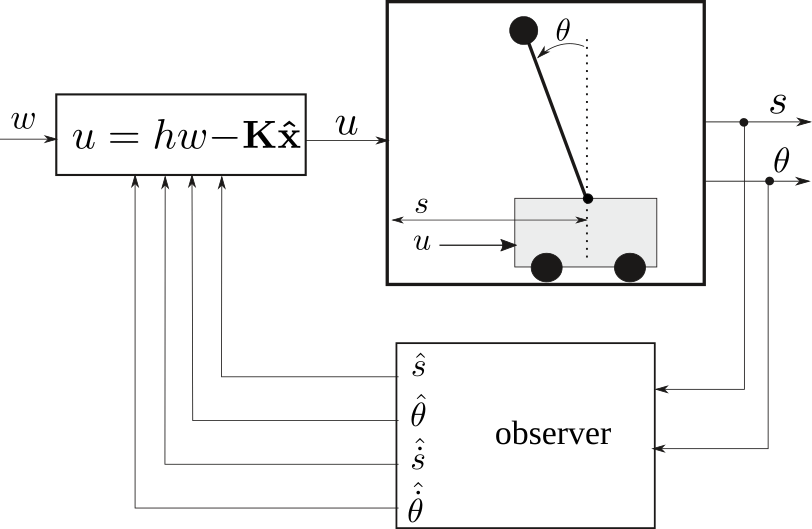
\includegraphics[width=7.5cm]{pendule_inverse_obs}\caption{Kalman filter used to estimate the state of the inverted rod pendulum}

\label{fig:pendule_inverse_obs}
\end{figure}

Discretize the system using steps of $dt=0.1\sec$, then propose a
Kalman filter for observing the state.

4) Implement this filter and study the robustness of the Kalman observer
when the measurement noise is increased.

5) An extended Kalman filter can be obtained by replacing, in the
prediction step of the Kalman filter, the statement: 
\[
\mathbf{\hat{x}}_{k+1|k}=\mathbf{A}_{k}\mathbf{\hat{x}}_{k|k}+\mathbf{B}_{k}\mathbf{u}_{k}
\]
by: 
\[
\mathbf{\hat{x}}_{k+1|k}=\mathbf{\hat{x}}_{k|k}+\mathbf{f}\left(\mathbf{\hat{x}}_{k|k},\mathbf{u}_{k}\right)\cdot dt.
\]
Here we have replaced the prediction performed on the linearized model
by a prediction performed on the initial nonlinear model that is closer
to reality. Propose an implementation of this extended Kalman filter
on the inverted rod pendulum.

\rule{0.95\columnwidth}{1pt}

\begin{Exercice} \label{ex:kalman:suivi:bateau} Following a boat
with two radars \end{Exercice}

\textcolor{blue}{See the correction video at \href{https://youtu.be/FQSud487xIE}{https://youtu.be/FQSud487xIE}}

The movement of a boat that we are seeking to localize is described
by the state equations: 
\[
\left\{ \begin{array}{lll}
p_{x}\left(k+1\right) & = & p_{x}\left(k\right)+dt\cdot v_{x}\left(k\right)\\
v_{x}\left(k+1\right) & = & v_{x}\left(k\right)-dt\cdot v_{x}\left(k\right)+\alpha_{x}\left(k\right)\\
p_{y}\left(k+1\right) & = & p_{y}\left(k\right)+dt\cdot v_{y}\left(k\right)\\
v_{y}\left(k+1\right) & = & v_{y}\left(k\right)-dt\cdot v_{y}\left(k\right)+\alpha_{y}\left(k\right)
\end{array}\right.
\]
where $dt=0.01$ and $\alpha_{x}$ and $\alpha_{y}$ are Gaussian
white noises with variance matrix $dt$. The state vector is therefore
$\mathbf{x}=\left(p_{x},v_{x},p_{y},v_{y}\right)$.

1) Write a program that simulates the boat.

2) Two radars placed at $\mathbf{a}:\left(a_{x},a_{y}\right)=\left(0,0\right)$
and $\mathbf{b}:\left(b_{x},b_{y}\right)=\left(1,0\right)$ measure
the square of the distance to the boat. The observation equation is:
\[
\mathbf{y}_{k}=\underset{\mathbf{g}\left(\mathbf{x}_{k}\right)}{\underbrace{\left(\begin{array}{c}
\left(p_{x}\left(k\right)-a_{x}\right)^{2}+\left(p_{y}\left(k\right)-a_{y}\right)^{2}\\
\left(p_{x}\left(k\right)-b_{x}\right)^{2}+\left(p_{y}\left(k\right)-b_{y}\right)^{2}
\end{array}\right)}}\ +\ \mathbf{\boldsymbol{\beta}}_{k}
\]
where $\beta_{1}\left(k\right)$ and $\beta_{2}\left(k\right)$ are
independent Gaussian white noises with a variance equal to $\frac{1}{dt}\cdot10^{-2}$.
Adjust the simulation in order to visualize the radars and generate
the measurement vector $\mathbf{y}\left(k\right)$.

3) Linearize this observation equation around the current estimation
$\mathbf{\hat{x}}_{k}$ of the state vector $\mathbf{x}_{k}$. Deduce
from this an equation of the form $\mathbf{z}_{k}=~\mathbf{C}_{k}\mathbf{x}_{k}$
where $\mathbf{z}_{k}=\mathbf{h}\left(\mathbf{y}_{k},\mathbf{\hat{x}}_{k}\right)$
takes the role of the measurement taken at time $k$.

4) Implement a Kalman filter that allows the localization of the boat.

\rule{0.95\columnwidth}{1pt}

\begin{Exercice} Robot localization in a pool \label{exer:locpool}
\end{Exercice}

\textcolor{blue}{See the correction video at \href{https://youtu.be/U3X52L9quvE}{https://youtu.be/U3X52L9quvE}}

Consider an underwater robot moving within a rectangular pool of length
$2R_{y}$ and width $2R_{x}$. A sonar placed at the center of the
robot rotates with a constant angular speed $\dot{\delta}$. The depth
is easily obtained using a barometer and we will therefore assume
this quantity to be known. The robot is weighted in such a way that
the bank and elevation angles may be assumed to be zero. We want to
estimate the coordinates $(x,y)$ of the robot. The origin of the
coordinate system is in middle of the pool. For this localization,
we will assume that the angle $\delta$ of the sonar is known perfectly
relative to the body of the robot and the heading angle $\theta$
is measured with a compass. The sonar illuminates the environment
inside an emission cone with an angle $\pm\frac{\pi}{4}$, as illustrated
by Figure \ref{fig:locpool0}.

\begin{figure}[H]
\centering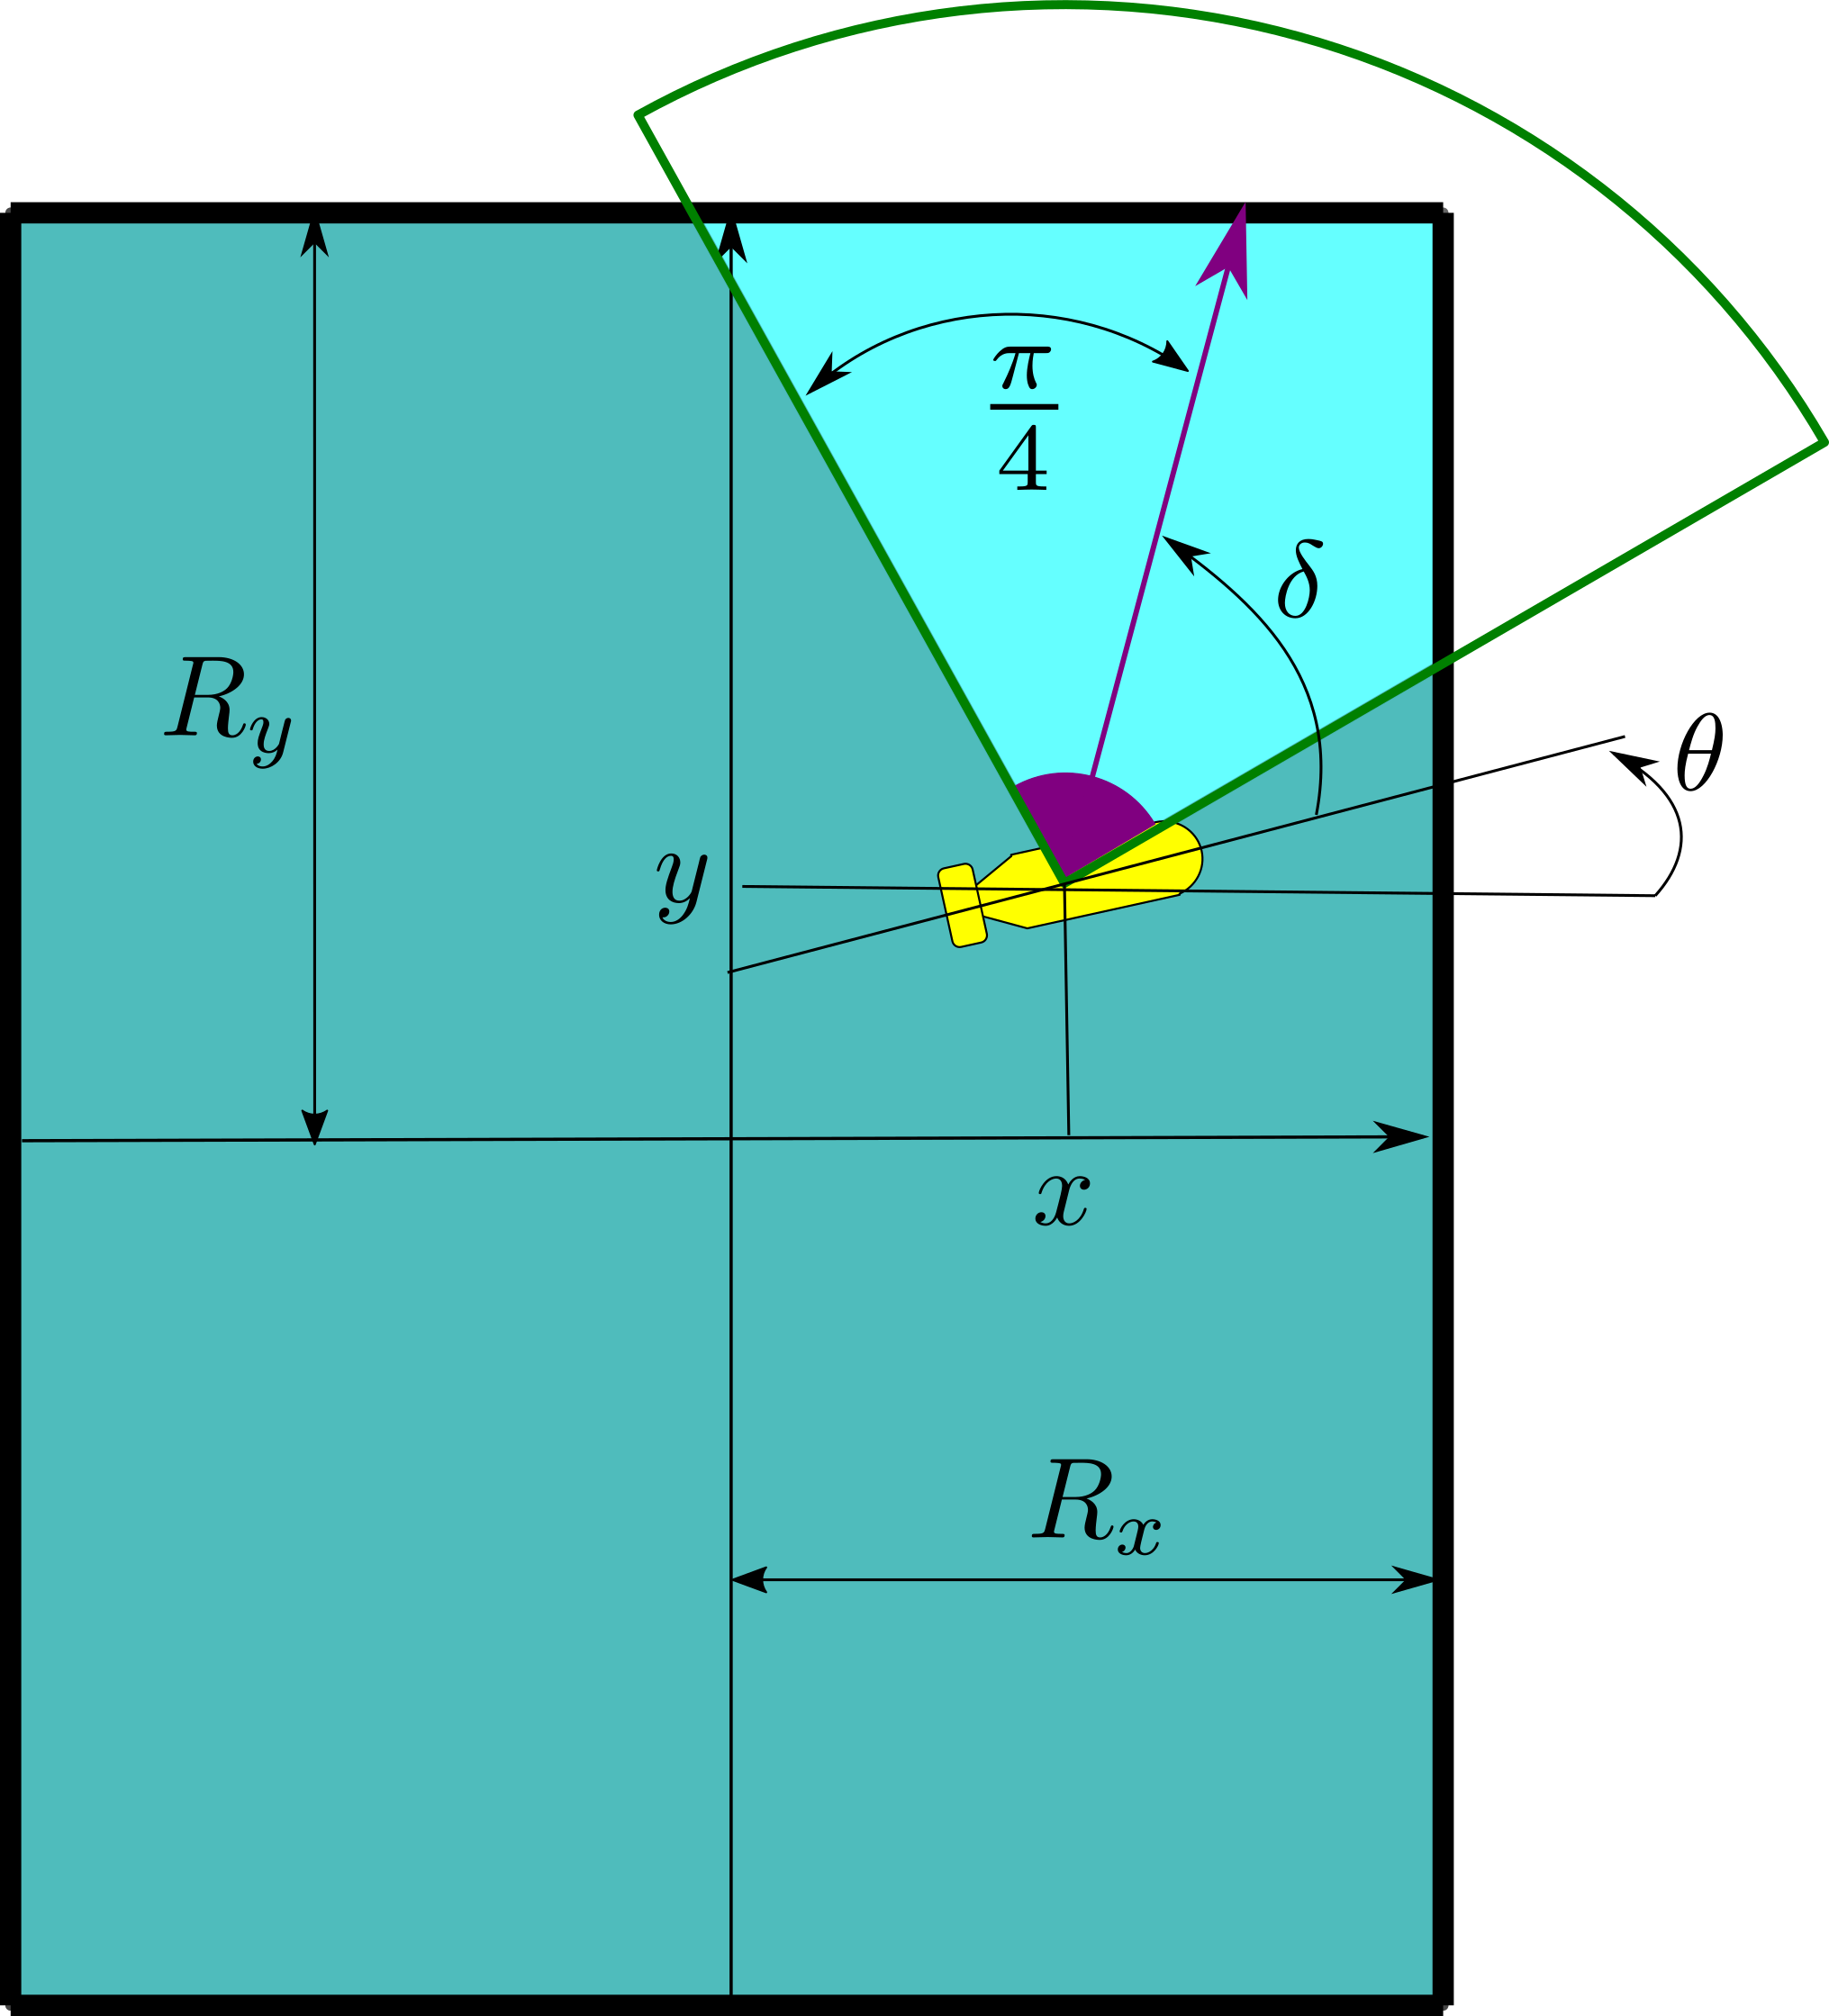
\includegraphics[width=6cm]{locpool0}\caption{In the pool, the rotating sonar measures the distance to one of the
wall}

\label{fig:locpool0}
\end{figure}

The tangential acceleration $a$ is measured with an accelerometer.
Every $dt=0.05$s, the sonar returns the distance $\ell$ to the wall
in front of it. As illustrated by Figure \ref{fig:locpool1} the number
$w$ of the wall involved in the distance measurement (called the
\emph{hit wall}) only depends on the angle $\theta+\delta$ and not
on the position of the robot. In the configuration (a) of Figure \ref{fig:locpool1}
right, the sonar in on the right of the robot and since $\theta+\delta\simeq\frac{\pi}{2}$,
Wall 1 is hit. In the configuration (b), the sonar is on the left
of the robot and since $\theta+\delta\simeq\pi$, Wall 2 is hit. 

\begin{figure}[H]
\centering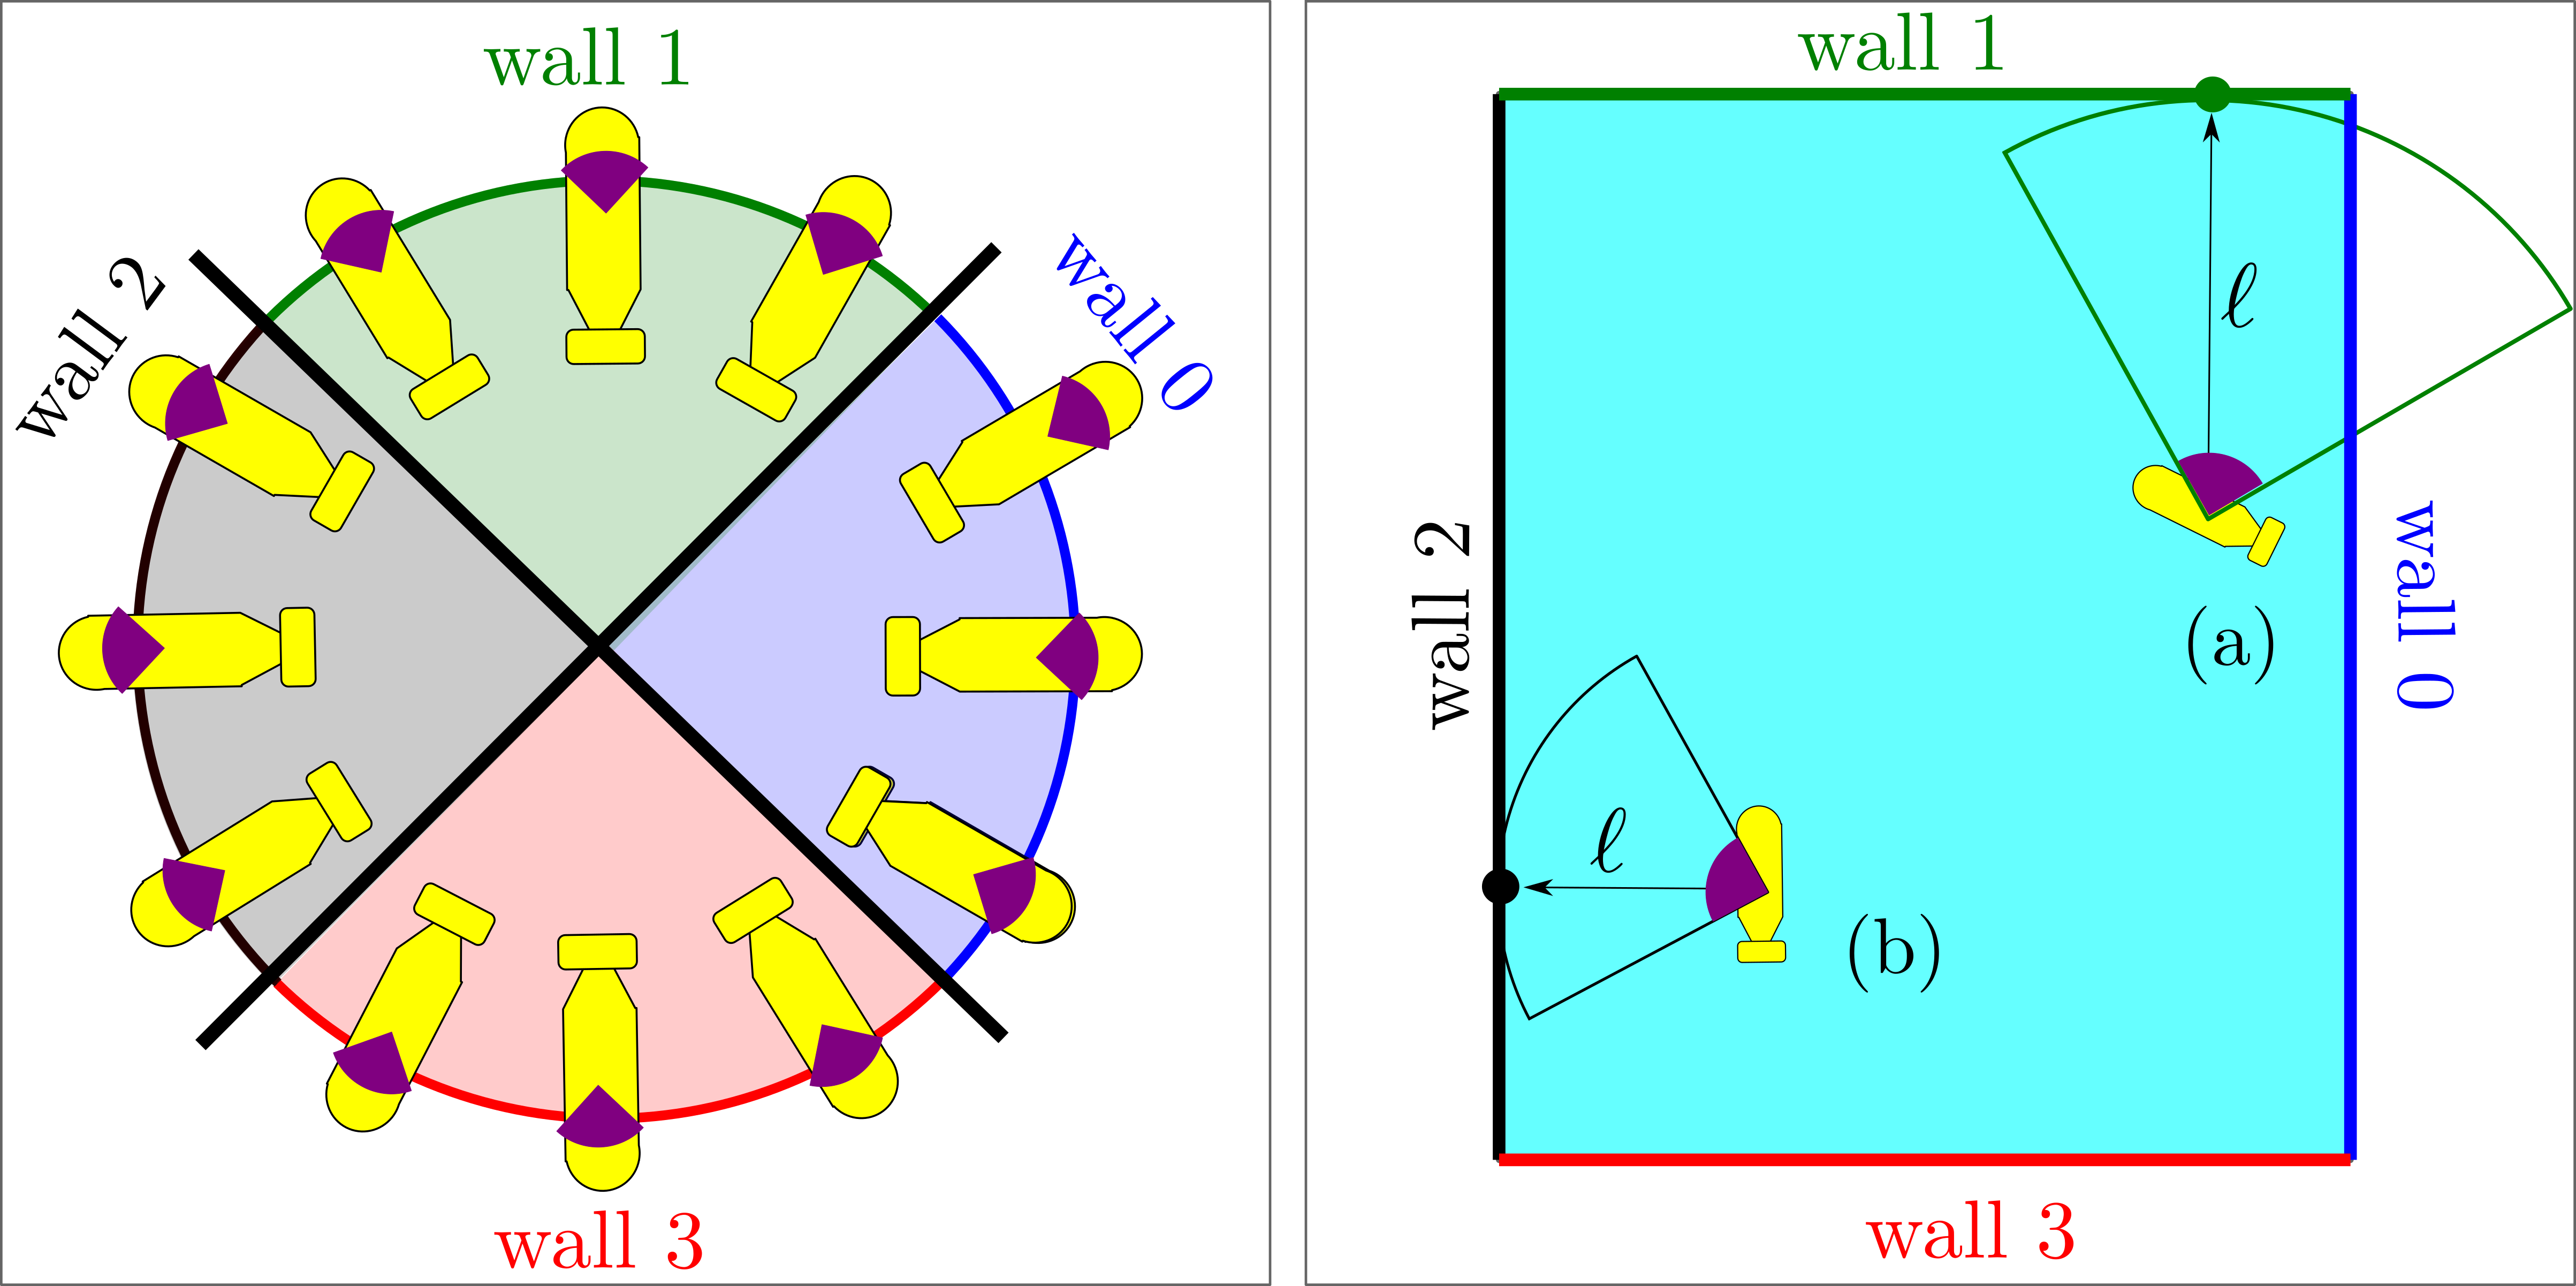
\includegraphics[width=13cm]{locpool1}\caption{The sonar returns the distance $\ell$ to the $w$th wall where $w$
depends on the orientation $\theta+\delta$ of the sonar }

\label{fig:locpool1}
\end{figure}

We want the build a Kalman filter which estimates the position $(x,y)$
from the measurements $a_{k},\ell_{k},\theta_{k},\delta_{k}$ at time
$t_{k}=dt\cdot k$.

\begin{figure}[H]
\centering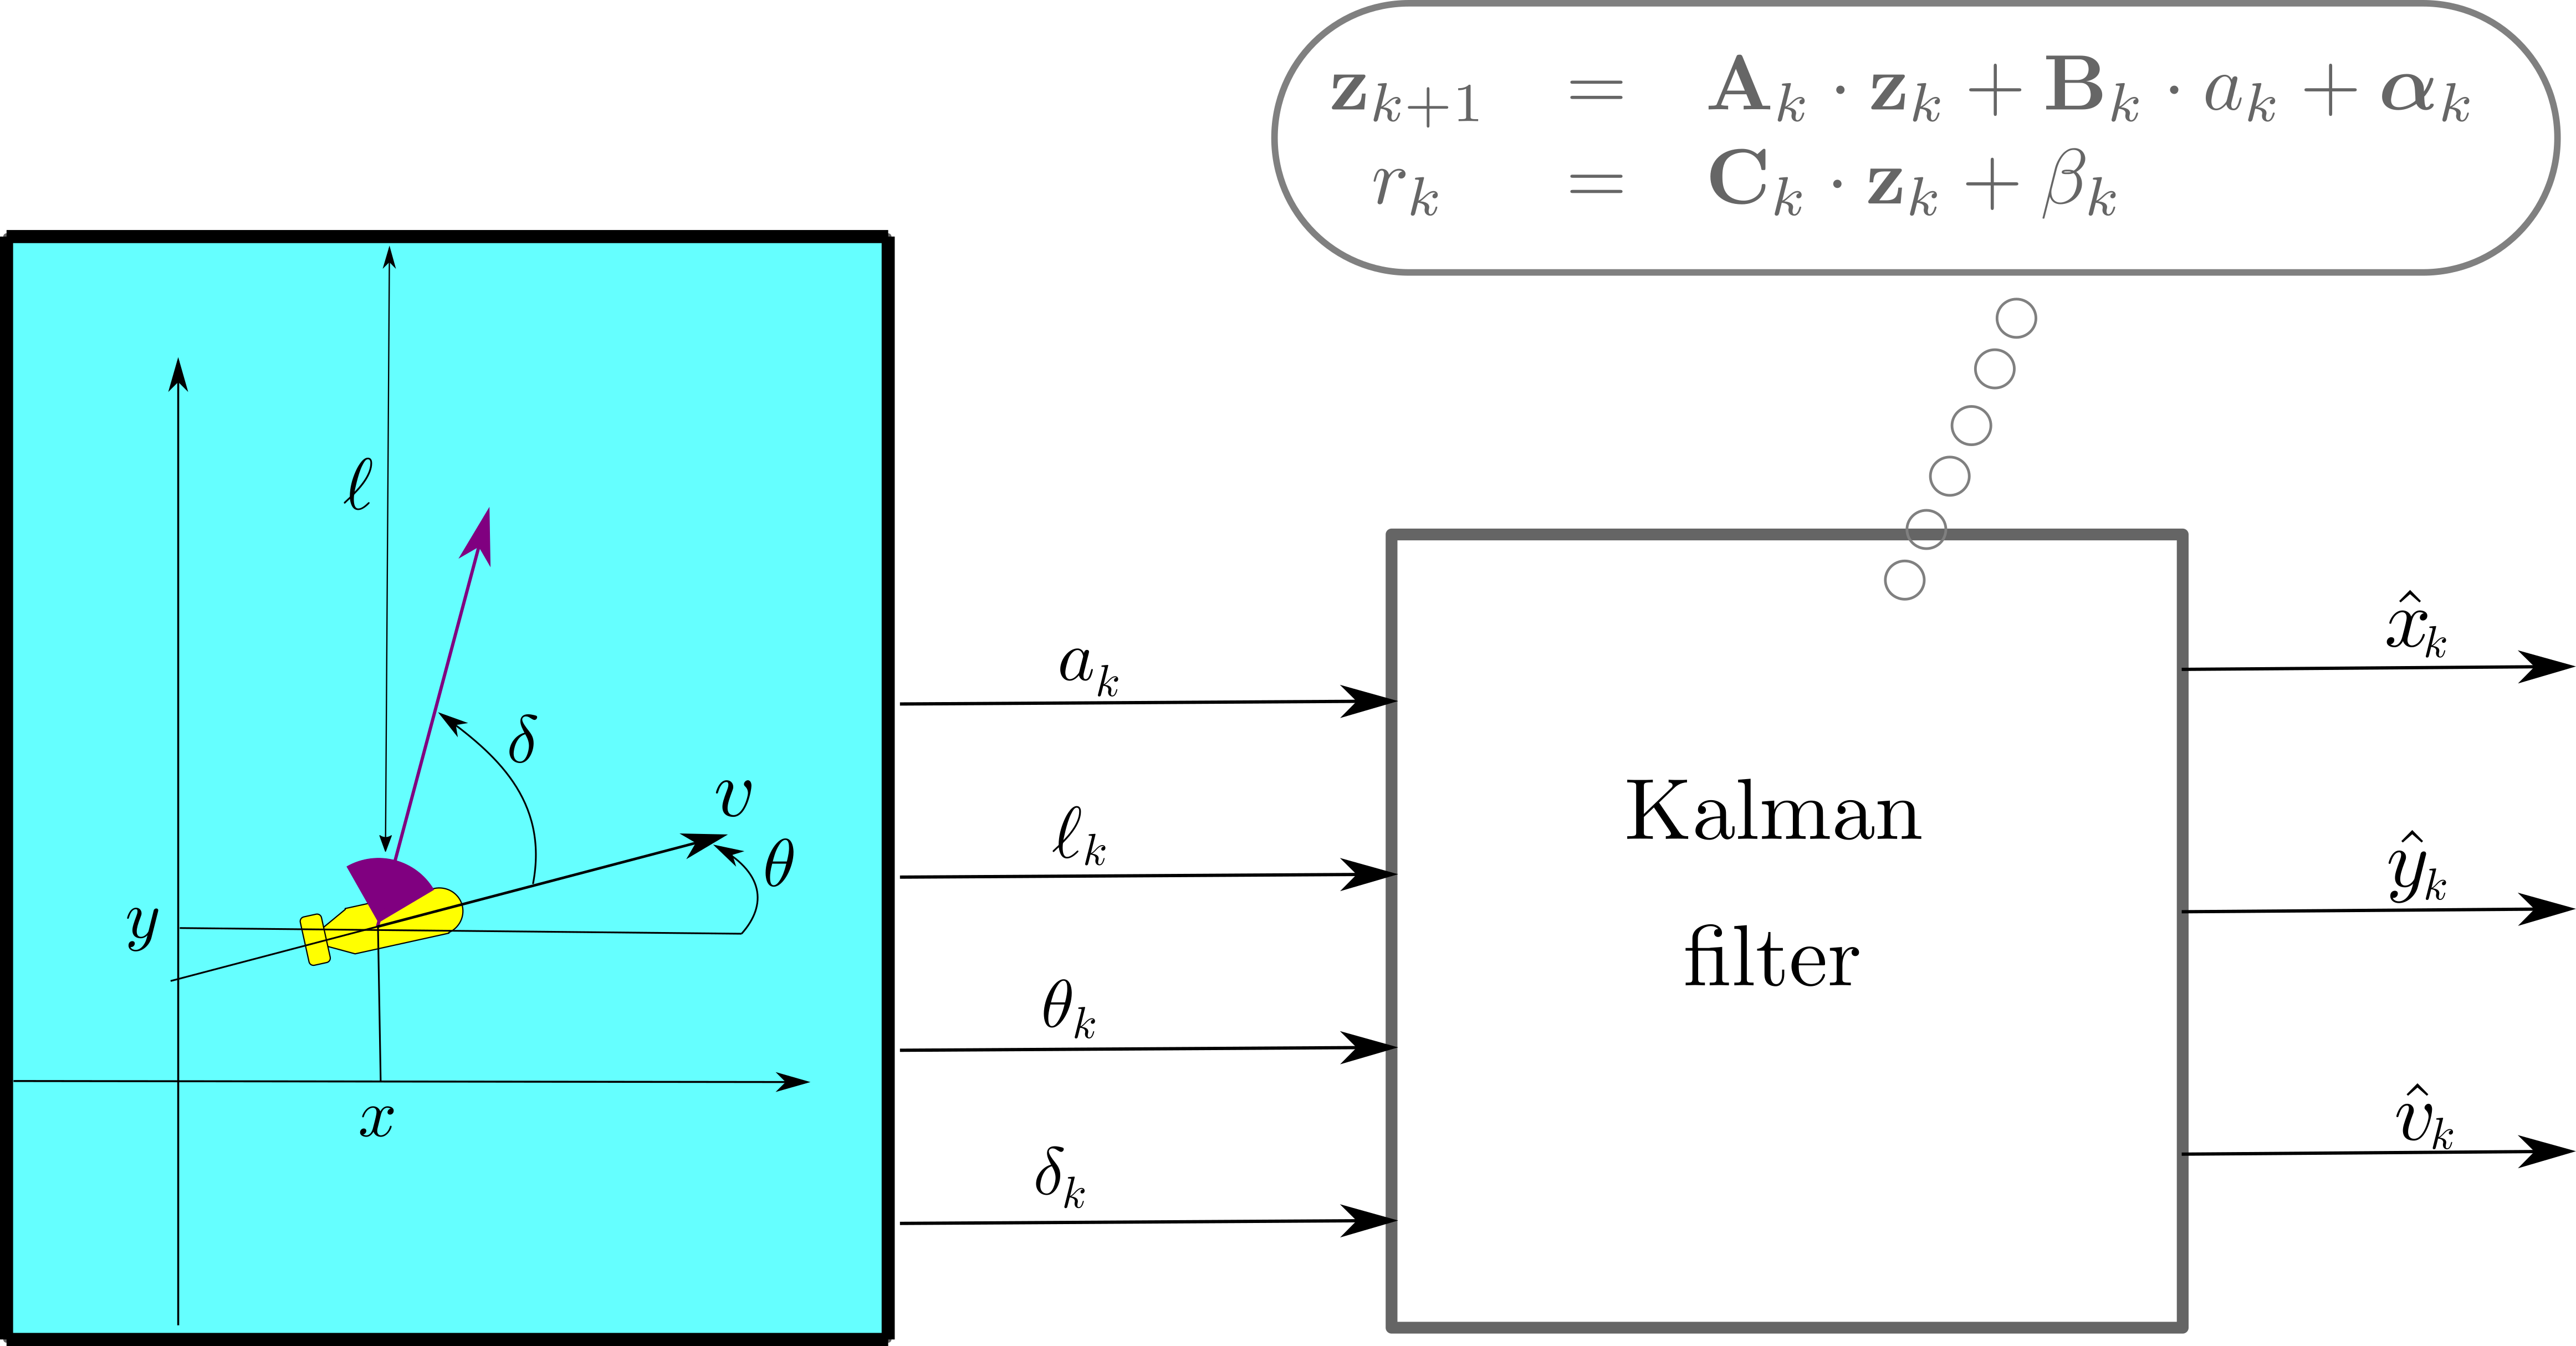
\includegraphics[width=13cm]{locpool2}\caption{The Kalman filter estimates the position of the robot in the pool
from the measurements collected by the sensors }

\label{fig:locpool1-1}
\end{figure}

The Kalman filter will be built on the following cinematic model 
\[
\left\{ \begin{array}{lll}
\dot{x} & = & v\cdot\cos\theta\\
\dot{y} & = & v\cdot\sin\theta\\
\dot{v} & = & a
\end{array}\right.
\]
The state vector is $\mathbf{z}=(x,y,v)$ and the input is $a$.

1) The Kalman filter assumes the following linear state equations
\[
\begin{array}{cll}
\mathbf{z}_{k+1} & = & \mathbf{A}_{k}\cdot\mathbf{z}_{k}+\mathbf{B}_{k}\cdot a_{k}+\mathbf{\boldsymbol{\alpha}}_{k}\\
r_{k} & = & \mathbf{C}_{k}\cdot\mathbf{z}_{k}+\beta_{k}
\end{array}
\]
where $\mathbf{\boldsymbol{\alpha}}_{k}$ and $\beta_{k}$ are white
Gaussian noises. Give the expressions for $\mathbf{A}_{k},\mathbf{B}_{k}$
and $\mathbf{C}_{k}$ we should take to have the estimations $\hat{x},\,\hat{y},\,\hat{v}$
of the variables $x,\,y,\,v$. Explain how the quantity $r_{k}$ should
be chosen from the measurements.

2) Simulate a robot in the pool. Its motion will obey to the state
equation

\[
\begin{array}{ccc}
\dot{x} & = & v\cdot\cos\theta\\
\dot{y} & = & v\cdot\sin\theta\\
\dot{\theta} & = & u_{1}\\
\dot{v} & = & u_{2}\\
\dot{\delta} & = & u_{3}
\end{array}
\]
The initial state vector $\mathbf{x}_{0}$ and the constant input
$\mathbf{u}$ are given by
\[
\mathbf{x}_{0}=\left(\begin{array}{c}
10\\
-10\\
1\\
3\\
0
\end{array}\right)\text{ and }\mathbf{u}=\left(\begin{array}{c}
0.2\\
0\\
2
\end{array}\right)
\]
Illustrate the behavior of the Kalman filter. To avoid outliers, we
will assume that the distance $\ell$ is reliable only when the sonar
beam is orthogonal to the hit wall.

\rule{0.95\columnwidth}{1pt}

\begin{Exercice} \label{ex:estim:etat:quasistat} Instantaneous state
estimation \end{Exercice}

\textcolor{blue}{See the correction video at \href{https://youtu.be/-JIQb_0CEI4}{https://youtu.be/-JIQb\_0CEI4}}

Localization consists of finding the position and the orientation
of the robot. This problem can sometimes be reduced to a state estimation
problem, if the state model for our robot is available. In this exercise,
we will give a method that is sometimes used for the state estimation
of nonlinear systems. Let us consider the tricycle described by the
state equations: 
\[
\left(\begin{array}{l}
\dot{x}\\
\dot{y}\\
\dot{\theta}\\
\dot{v}\\
\dot{\delta}
\end{array}\right)=\left(\begin{array}{c}
v\cos\delta\cos\theta\\
v\cos\delta\sin\theta\\
v\sin\delta\\
u_{1}\\
u_{2}
\end{array}\right)
\]
\begin{figure}[H]
\centering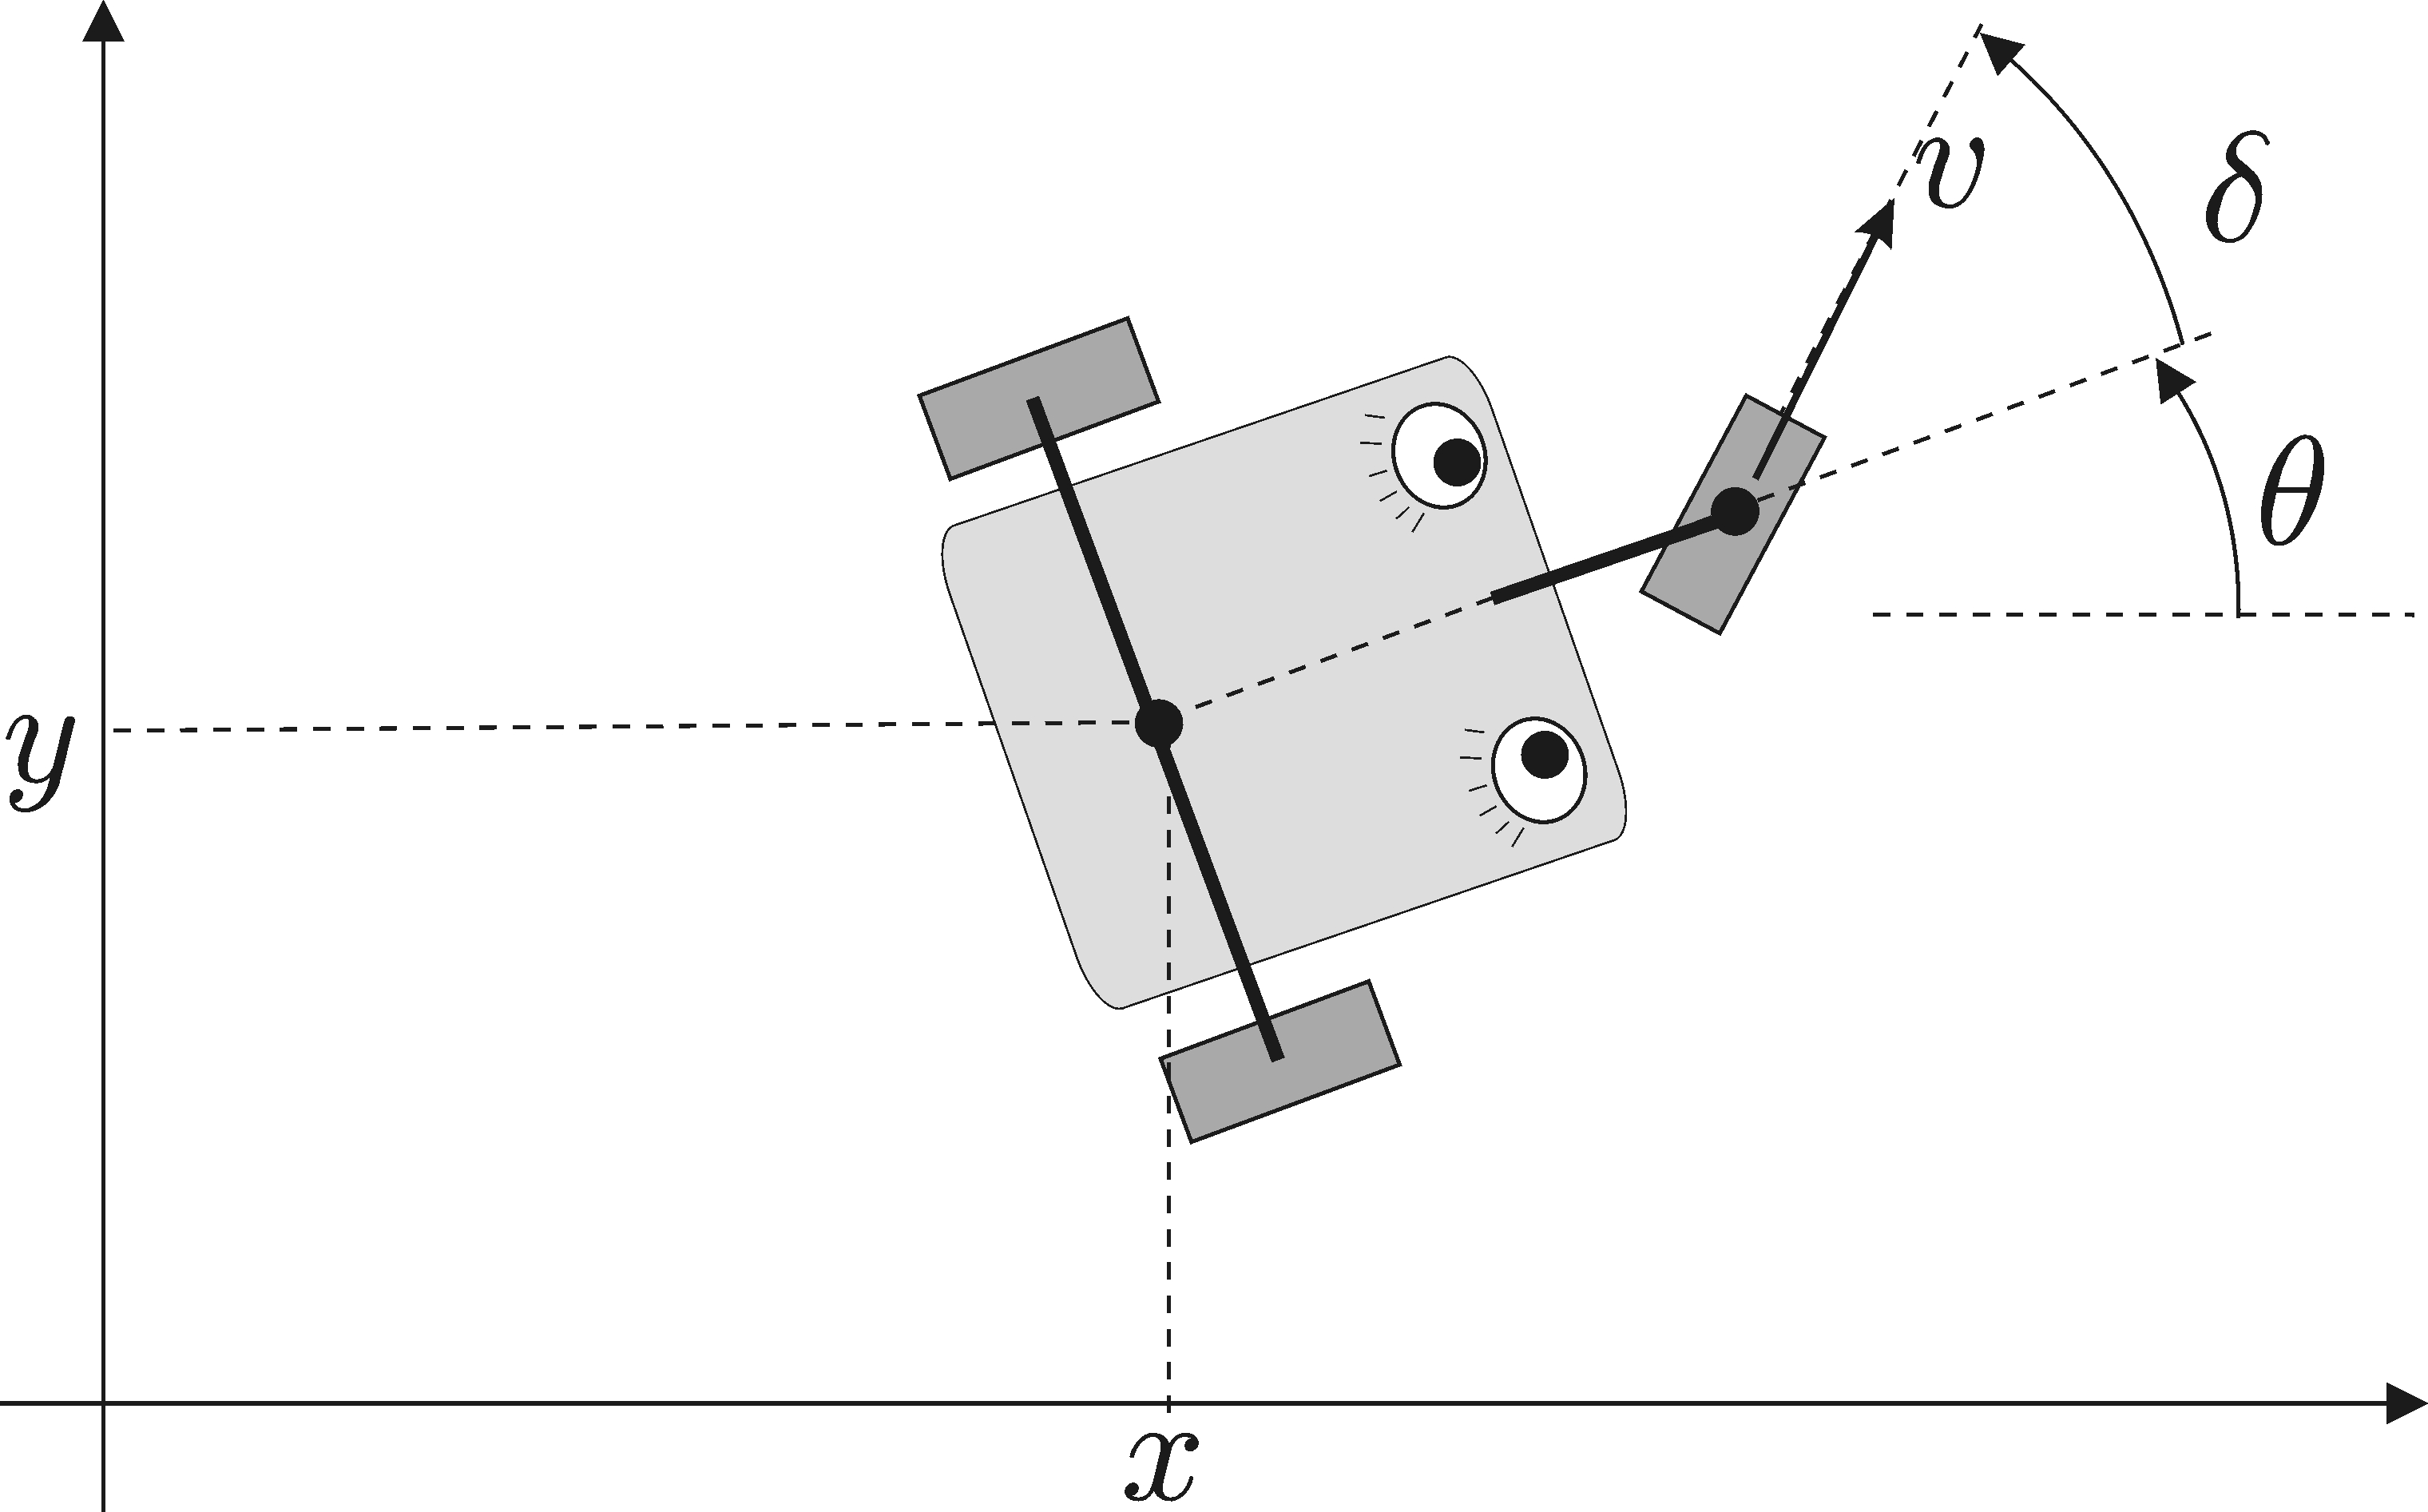
\includegraphics[width=6cm]{robot_tricycle}\caption{Tricycle for which we want to reconstruct the state}

\label{fig:robot:tricycle}
\end{figure}
We measure the positions $x$ and $y$ with such high precision that
we may assume that $\dot{x},\dot{y},\ddot{x},\ddot{y}$ are known.
Express the other state variables $\theta,v,\delta$ in function of
$x$,$y$,$\dot{x}$,$\dot{y}$,$\ddot{x}$,$\ddot{y}$.


\chapter{Bayes filter\label{chap:Bayes-filter}}

\section{Introduction}

This chapter proposes to generalize the Kalman filter to the case
where the functions are nonlinear and the noise is non Gaussian. The
resulting observer will be called the \emph{Bayes filter}. Instead
of computing for each time $k$ the covariance and the estimate of
the state, the Bayes filter directly computes the probability density
function of the state vector. As for the Kalman filter, it consists
of two parts: the prediction and the correction. In the linear and
Gaussian case, the Bayes filter is equivalent to the Kalman filter.

By increasing the level of abstraction, the Bayes filter will allow
us to have a better understanding of the Kalman filter, and some proofs
become easier and more intuitive. As an illustration we will consider
the smoothing problem where the estimation is made more accurate by
taking all future measurements, when available. Of course, the smoothing
is mainly used for offline applications.

\section{Basic notions on probabilities}

\textbf{Marginal density}. If $\mathbf{x}\in\mathbb{R}^{n}$ and $\mathbf{y}\in\mathbb{R}^{m}$
are two random vectors with a joint probability density function $\pi(\mathbf{x},\mathbf{y})$.
Note that $\pi(\mathbf{x},\mathbf{y})$ is a function which associates
to $\left(\mathbf{\tilde{x},\tilde{y}}\right)\in\mathbb{R}^{n}\times\mathbb{R}^{m}$
an element of $\mathbb{R}^{+}$ denoted by $\pi(\mathbf{x=\tilde{x}},\mathbf{y=\tilde{y}})$.
The \emph{marginal density} for $\mathbf{x}$ is
\begin{equation}
\pi(\mathbf{x})=\int\pi(\mathbf{x},\mathbf{y})\cdot d\mathbf{y}.\label{eq:loi:marginale:x}
\end{equation}
Note that, to be rigorous, we should have written
\[
\pi(\mathbf{x=\tilde{x}})=\int_{\mathbf{\tilde{y}\in}\mathbb{R}^{m}}\pi(\mathbf{x=\tilde{x}},\mathbf{y=\tilde{y}})\cdot d\mathbf{\tilde{y}},
\]
but this notation would become too heavy for our applications. In
the same manner, the marginal density for $\mathbf{y}$ is 
\[
\pi(\mathbf{y})=\int\pi(\mathbf{x},\mathbf{y})\cdot d\mathbf{x}.
\]
The two random vectors $\mathbf{x}$ and $\mathbf{y}$ are \emph{independent}
if 
\[
\pi(\mathbf{x},\mathbf{y})=\pi(\mathbf{x})\cdot\pi(\mathbf{y}).
\]
\textbf{Conditional density}. The \emph{conditional density} for $\mathbf{x}$
given $\mathbf{y}$ is 
\begin{equation}
\pi(\mathbf{x}|\mathbf{y})=\frac{\pi(\mathbf{x\textnormal{,}y})}{\pi(\mathbf{y})}.\label{eq:pi:de:x:sachant:y}
\end{equation}
Again, the quantity $\pi(\mathbf{x}|\mathbf{y})$ is a function which
associates with the pair $\left(\mathbf{\tilde{x},\tilde{y}}\right)\in\mathbb{R}^{n}\times\mathbb{R}^{m}$
a positive real number. But, $\mathbf{y}$ has not the same role:
it is a parameter of the density for $\mathbf{x}$. We also have
\begin{equation}
\pi(\mathbf{y}|\mathbf{x})=\frac{\pi(\mathbf{x\textnormal{,}y})}{\pi(\mathbf{x})}.\label{eq:pi:de:y:sachant:x}
\end{equation}
\textbf{Bayes rule}. Combining the two equations (\ref{eq:pi:de:x:sachant:y})
and (\ref{eq:pi:de:y:sachant:x}), we get
\[
\pi(\mathbf{x\textnormal{,}y})=\pi(\mathbf{y}|\mathbf{x})\cdot\pi(\mathbf{x})=\pi(\mathbf{x}|\mathbf{y})\cdot\pi(\mathbf{y}).
\]
The\emph{ Bayes} \emph{rule} obtained from the previous equation:
\begin{equation}
\pi(\mathbf{x}|\mathbf{y})=\frac{\pi(\mathbf{y}|\mathbf{x})\cdot\pi(\mathbf{x})}{\pi(\mathbf{y})}=\eta\cdot\pi(\mathbf{y}|\mathbf{x})\cdot\pi(\mathbf{x}).\label{eq:regle:bayes}
\end{equation}
The quantity $\eta=\frac{1}{\pi(\mathbf{y})}$ called the \emph{normalizer}
allows to have an integral for $\mathbf{x}$ equal to one. Sometimes,
we use the following notation
\[
\pi(\mathbf{x}|\mathbf{y})\propto\pi(\mathbf{y}|\mathbf{x})\cdot\pi(\mathbf{x})
\]
to indicate that the two functions $\pi(\mathbf{x}|\mathbf{y})\ $and
$\pi(\mathbf{y}|\mathbf{x})\cdot\pi(\mathbf{x})$ are proportional
for a given $\mathbf{y}$.

\textbf{Total probability law}. The marginal density for $\mathbf{x}$
is
\begin{equation}
\pi(\mathbf{x})\overset{\text{(\ref{eq:loi:marginale:x},\ref{eq:pi:de:x:sachant:y})}}{=}\int\pi(\mathbf{x}|\mathbf{y})\cdot\pi(\mathbf{y})\cdot d\mathbf{y}.\label{eq:total:density}
\end{equation}
This corresponds to the \emph{law of total probability}. 

\textbf{Parametric case}. If $\mathbf{z}$ is a parameter (which can
be random vector and any other deterministic quantity), the parametric
total probability law is given by 
\begin{equation}
\pi(\mathbf{x|z})\overset{(\ref{eq:total:density})}{=}\int\pi(\mathbf{x}|\mathbf{y\textnormal{,}z})\cdot\pi(\mathbf{y|z})\cdot d\mathbf{y}\label{eq:th:proba:totale:cond}
\end{equation}
and the parametric Bayes rule is
\begin{equation}
\pi(\mathbf{x}|\mathbf{y,z})\overset{(\ref{eq:regle:bayes})}{=}\frac{\pi(\mathbf{y}|\mathbf{x\textnormal{,}z})\cdot\pi(\mathbf{x|z})}{\pi(\mathbf{y|z})}.\label{eq:Bayes:cond}
\end{equation}

\textbf{Bayes network}. A Bayes network is a probabilistic graphical
model that represents a set of random vectors and their conditional
dependencies. Formally, Bayes networks are directed acyclic graph
whose nodes represent random vectors. Arcs represent dependencies.
More precisely the two vectors $\mathbf{x},\mathbf{y}$ are connected
by an arc there exists a relation linking them. Nodes that are not
connected (there is no path from one of the variables to the other
in the Bayes network) represent variables that are independent. To
have a better understanding, consider five vectors $\mathbf{a},\mathbf{b},\mathbf{c},\mathbf{d},\mathbf{e}$
that are linked by the relations
\[
\begin{array}{ccc}
\mathbf{b} & = & \mathbf{a}+\boldsymbol{\alpha}_{1}\\
\mathbf{e} & = & \mathbf{a}+2\mathbf{b}+\boldsymbol{\alpha}_{2}\\
\mathbf{c} & = & \mathbf{e}+\boldsymbol{\alpha}_{3}\\
\mathbf{d} & = & 3\mathbf{c}+\boldsymbol{\alpha}_{4}
\end{array}
\]
where the $\boldsymbol{\alpha}_{i}$ are all independent vectors with
a known density, for instance $\mathcal{N}(0,1)$, which means Gaussian
centered with a unit variance. It is clear that if we know a density
$\pi(\mathbf{a})$ for $\mathbf{a}$, we can compute the probabilities
for all other vectors. Equivalently, we can easily write a program
which generates the generates some realizations for all the vectors.
For instance in the scalar case, if $\pi(a)=\mathcal{N}(1,9)$, the
program could be:
\begin{singlespace}
\begin{center}
\begin{tabular}{|cl|}
\hline 
1 & $a:=1+$randn$(9)$\tabularnewline
2 & $b:=a+\text{randn}(1)$\tabularnewline
3 & $e:=a+2\cdot b+\text{randn}(1)$\tabularnewline
4 & $c:=e+\text{randn}(1);$\tabularnewline
5 & $d:=3\cdot c+\text{randn}(1)$\tabularnewline
\hline 
\end{tabular}
\par\end{center}
\end{singlespace}

From this program, we easily see that $\pi(\mathbf{c}|\mathbf{a},\mathbf{e},\mathbf{b})=\pi(\mathbf{c}|\mathbf{e})$,
which means that given $\mathbf{e}$, the vector $\mathbf{c}$ is
independent of $\mathbf{a}$ and $\mathbf{b}$. The corresponding
network is depicted on Figure \ref{fig:bayes_net1} (left). The network
will help us to simplify conditional densities. For instance, from
the network we can conclude that $\pi(\mathbf{c}|\mathbf{a},\mathbf{e},\mathbf{b})=\pi(\mathbf{c}|\mathbf{e})$,
since all paths from $\mathbf{a}$ to $\mathbf{c}$ and all paths
from $\mathbf{b}$ to $\mathbf{c}$ have to go through $\mathbf{e}$.
Equivalently, this means that if we know $\mathbf{e}$, the knowledge
of $\mathbf{a}$ and $\mathbf{b}$ does not bring any new information
on $\mathbf{c}$. This reasoning can be formalized and generalized
under the form of the Hammersley\textendash Clifford theorem.

Consider 3 vectors $\mathbf{x},\mathbf{y},\mathbf{z}$ that are linked
by the relations
\[
\begin{array}{ccc}
\mathbf{y} & = & 2\mathbf{x}+\boldsymbol{\alpha}_{1}\\
\mathbf{z} & = & 3\mathbf{y}+\boldsymbol{\alpha}_{2}\\
\mathbf{x} & = & 4\mathbf{z}+\boldsymbol{\alpha}_{3}
\end{array}
\]
where the $\boldsymbol{\alpha}_{i}$ are all independent vectors.
The graph (see Figure \ref{fig:bayes_net1} (right) has a cycle and
is not considered as a Bayes network anymore. It is now much more
difficult (or even impossible) to compute the marginal densities or
to build a program that generates a cloud of points consistent with
the probabilistic assumptions.

\begin{figure}[H]
\centering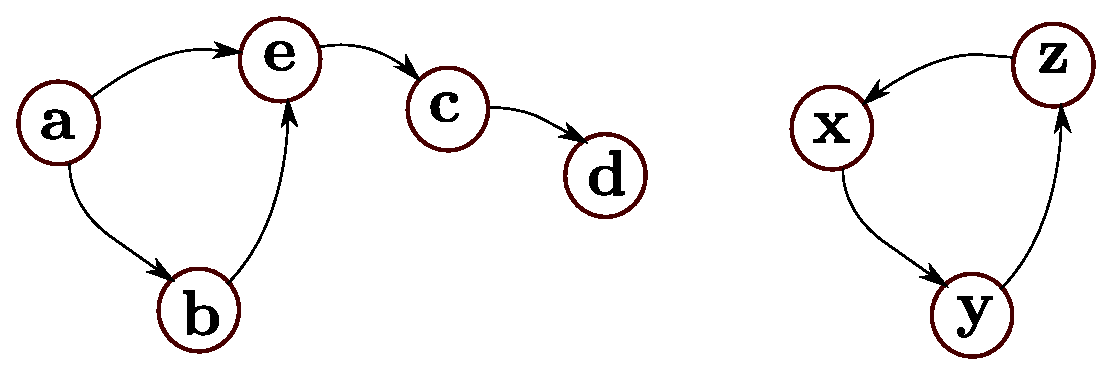
\includegraphics[width=8cm]{bayes_net1}\caption{Left: a Bayes network; Right, the graph has a cycle and thus is not
a Bayes network}

\label{fig:bayes_net1}
\end{figure}


\section{Bayes filter}

Consider a system described by the following state equations
\begin{equation}
\left\{ \begin{array}{ccc}
\mathbf{x}_{k+1} & = & \mathbf{f}_{k}(\mathbf{x}_{k})+\boldsymbol{\alpha}_{k}\\
\mathbf{y}_{k} & = & \mathbf{g}_{k}(\mathbf{x}_{k})+\boldsymbol{\beta}_{k}
\end{array}\right.\label{eq:equations:etat}
\end{equation}
where $\boldsymbol{\alpha}_{k}$ and $\boldsymbol{\beta}_{k}$ are
random vectors white and mutually independent. The dependency with
respect to some known inputs $\mathbf{u}_{k}$ is taken into account
via the functions $\mathbf{f}_{k}$ and $\mathbf{g}_{k}$.\textbf{\ }We
have here a random process which satisfies the Markov assumptions
which tells us that the future of the system only depends of the past
through the state at the current time $t$. This can be written as:
\begin{equation}
\begin{array}{lll}
\pi(\mathbf{y}_{k}|\mathbf{x}_{k},\mathbf{y}_{0:k-1}) & = & \pi(\mathbf{y}_{k}|\mathbf{x}_{k})\\
\pi(\mathbf{x}_{k+1}|\mathbf{x}_{k},\mathbf{y}_{0:k}) & = & \pi(\mathbf{x}_{k+1}|\mathbf{x}_{k}).
\end{array}\label{eq:hyp:markov}
\end{equation}
The notation $\mathbf{y}_{0:k}$ has to be understood as follows
\[
\mathbf{y}_{0:k}=\left(\mathbf{y}_{0},\mathbf{y}_{1},\dots,\mathbf{y}_{k}\right).
\]

This is illustrated by the Bayes network of Figure \ref{fig:bayes_net2}.
An arc of this graph corresponds to a dependency. For instance, the
arc between $\mathbf{x}_{k}$ and $\mathbf{x}_{k+1}$ corresponds
to the knowledge that $\mathbf{x}_{k+1}-\mathbf{f}_{k}(\mathbf{x}_{k})$
has a density which corresponds to that of $\boldsymbol{\alpha}_{k}$.

\begin{figure}[H]
\centering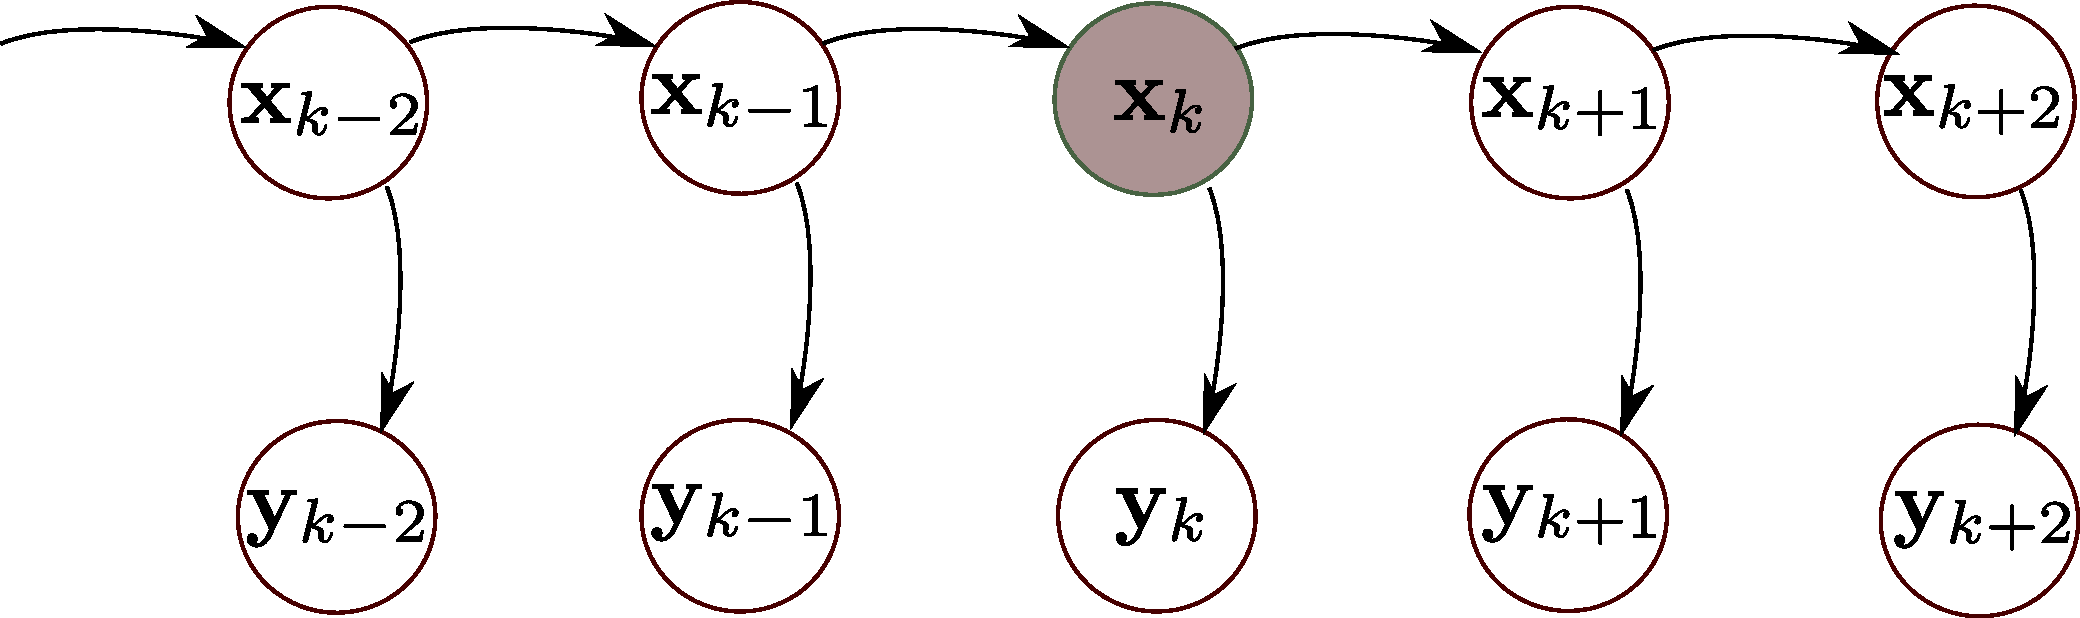
\includegraphics[width=8cm]{bayes_net2}\caption{Bayes network associated with the state equation}

\label{fig:bayes_net2}
\end{figure}

\begin{thm}
The two densities 
\begin{equation}
\begin{array}{lll}
\text{pred}(\mathbf{x}_{k}) & \overset{\text{def}}{=} & \pi(\mathbf{x}_{k}|\mathbf{y}_{0:k-1})\\
\text{bel}(\mathbf{x}_{k}) & \overset{\text{def}}{=} & \pi(\mathbf{x}_{k}|\mathbf{y}_{0:k}).
\end{array}\label{eq:pred:bel:def}
\end{equation}
satisfy
\begin{equation}
\begin{array}{lllll}
\text{(i)} & \text{pred}\left(\mathbf{x}_{k+1}\right) & = & \int\pi\left(\mathbf{x}_{k+1}|\mathbf{x}_{k}\right)\cdot\text{bel}\left(\mathbf{x}_{k}\right)\cdot d\mathbf{x}_{k} & \text{ (prediction)}\\
\text{(ii)} & \text{bel}\left(\mathbf{x}_{k}\right) & = & \frac{\pi(\mathbf{y}_{k}|\mathbf{x}_{k})\cdot\text{pred}\left(\mathbf{x}_{k}\right)}{\pi\left(\mathbf{y}_{k}|\mathbf{y}_{0:k-1}\right)}. & \text{(correction)}
\end{array}\label{eq:pred:bel}
\end{equation}
\end{thm}
These relations correspond to a \emph{Bayes observer} or \emph{Bayes}
\emph{filter}. The prediction equation is known as the equation of
\emph{Chapman-Kolmogorov}. 
\begin{proof}
Let us prove relation (ii). We have 
\[
\begin{array}{lllcc}
\text{bel}\left(\mathbf{x}_{k}\right) & \overset{\text{(\ref{eq:pred:bel:def})}}{=} & \pi\left(\mathbf{x}_{k}|\mathbf{y}_{0:k}\right)\\
 & = & \pi\left({\color{magenta}\mathbf{x}_{k}}|\mathbf{y}_{k},{\color{green}\mathbf{y}_{0:k-1}}\right)\\
 & \overset{\text{(\ref{eq:Bayes:cond})}}{=} & \frac{1}{\pi\left(\mathbf{y}_{k}|{\color{green}\mathbf{y}_{0:k-1}}\right)}\cdot\underset{\overset{\text{(\ref{eq:hyp:markov})}}{=}\pi(\mathbf{y}_{k}|\mathbf{x}_{k})}{\underbrace{\pi(\mathbf{y}_{k}|{\color{magenta}\mathbf{x}_{k}},{\color{green}\mathbf{y}_{0:k-1}})}}\cdot\underset{\overset{\text{(\ref{eq:pred:bel:def})}}{=}\text{pred}\left(\mathbf{x}_{k}\right)}{\underbrace{\pi({\color{magenta}\mathbf{x}_{k}}|{\color{green}\mathbf{y}_{0:k-1}})}} & \,\,\,\, & \left\{ \pi({\color{magenta}\mathbf{x}}|\mathbf{y,{\color{green}z}})=\frac{\pi(\mathbf{y}|\mathbf{{\color{magenta}x},{\color{green}z}})\cdot\pi(\mathbf{{\color{magenta}x}|{\color{green}z}})}{\pi(\mathbf{y|{\color{green}z}})}\right\} 
\end{array}
\]
Let us now prove (i). From the\emph{ }total probability rule (\ref{eq:th:proba:totale:cond}),
we get
\[
\begin{array}[t]{lllcc}
\text{pred}\left(\mathbf{x}_{k+1}\right) & \overset{\text{(\ref{eq:pred:bel:def})}}{=} & \pi\left({\color{magenta}\mathbf{x}_{k+1}}|{\color{green}\mathbf{y}_{0:k}}\right)\\
 & \overset{\text{(\ref{eq:th:proba:totale:cond})}}{=} & \int\underset{\begin{array}{cc}
\overset{\text{(\ref{eq:hyp:markov})}}{=} & \pi(\mathbf{x}_{k+1}|\mathbf{x}_{k})\end{array}}{\underbrace{\pi({\color{magenta}\mathbf{x}_{k+1}}|{\color{red}\mathbf{x}_{k}},{\color{green}\mathbf{y}_{0:k}})}}\cdot\underset{\begin{array}{cc}
\overset{\text{(\ref{eq:pred:bel:def})}}{=} & \text{bel}\left(\mathbf{x}_{k}\right)\end{array}}{\underbrace{\pi({\color{red}\mathbf{x}_{k}}|{\color{green}\mathbf{y}_{0:k}})}}d{\color{red}\mathbf{x}_{k}} & \, & \begin{array}{clc}
\{ & \pi(\mathbf{{\color{magenta}x}|{\color{green}z}})=\\
 & \,\int\pi(\mathbf{{\color{magenta}x}}|\mathbf{{\color{red}y},{\color{green}z}})\cdot\pi(\mathbf{{\color{red}y}|{\color{green}z}})\cdot d\mathbf{{\color{red}y}} & \}
\end{array}
\end{array}
\]
This corresponds to relation (i).
\end{proof}
\textbf{Remark}. From (\ref{eq:pred:bel}, ii), we have
\[
\underset{=1}{\underbrace{\int\text{bel}\left(\mathbf{x}_{k}\right)\cdot d\mathbf{x}_{k}}}\ =\ \int\frac{\pi(\mathbf{y}_{k}|\mathbf{x}_{k})\cdot\text{pred}\left(\mathbf{x}_{k}\right)}{\pi\left(\mathbf{y}_{k}|\mathbf{y}_{0:k-1}\right)}\cdot d\mathbf{x}_{k}.
\]
Thus
\[
\pi\left(\mathbf{y}_{k}|\mathbf{y}_{0:k-1}\right)=\int\pi(\mathbf{y}_{k}|\mathbf{x}_{k})\cdot\text{pred}\left(\mathbf{x}_{k}\right)\cdot d\mathbf{x}_{k}
\]
is a normalizer coefficient which can be computed directly from $\pi(\mathbf{y}_{k}|\mathbf{x}_{k})$
and pred$\left(\mathbf{x}_{k}\right).$

The relations (\ref{eq:pred:bel}) can be interpreted as an algorithm
where the variables pred$\left(\mathbf{x}_{k}\right)$ and bel$\left(\mathbf{x}_{k}\right)$
are densities, \emph{i.e.}, functions from $\mathbb{R}^{n}\rightarrow\mathbb{R}$.
Such an algorithm cannot be implemented in a computer in the general
case, and can only be poorly approximated. In practice different approaches
can be used to implement a Bayes filter.
\begin{itemize}
\item If the random vector $\mathbf{x}$ is discrete, the process can be
represented by a Markov chain and the densities pred$\left(\mathbf{x}_{k}\right)$
and bel$\left(\mathbf{x}_{k}\right)$ can be represented by a vector
of $\mathbb{R}^{n}$. The Bayes filter can be implemented exactly.
\item If the densities pred$\left(\mathbf{x}_{k}\right)$ and bel$\left(\mathbf{x}_{k}\right)$
are Gaussian, they can be represented exactly by their expectation
and their covariance matrices. We get the Kalman filter \index{Kalman filter}
\cite{Kalman60}.
\item We can approximate pred$\left(\mathbf{x}_{k}\right)$ and bel$\left(\mathbf{x}_{k}\right)$
by cloud of points (called \emph{particles}) with different weights.
The corresponding observer is called \emph{Particle filter}.
\item We can represent the densities pred$\left(\mathbf{x}_{k}\right)$
and bel$\left(\mathbf{x}_{k}\right)$ with a subset of $\mathbb{R}^{n}$
which contains the support of the density. We obtain an observer called
\emph{set-membership filter}.
\end{itemize}

\section{Bayes smoother}

A filter is causal. This means that the estimation $\mathbf{\hat{x}}_{k|k-1}$
only takes into account the past. The \emph{smoothing}\index{smoothing}\index{Kalman smoother}
process consists of a state estimation when all the measurements (future,
present and past) are available. Let us denote by $N$ the maximum
time $k$. This time can correspond, for instance, to the end date
of a mission performed by the robot and for which we are trying to
estimate its path. In order to perform smoothing, we simply need to
run once more a Kalman filter in the backward direction and merge,
for each $k$, the information from the future with that of the past. 
\begin{thm}
The three densities 
\begin{equation}
\begin{array}{lll}
\text{pred}\left(\mathbf{x}_{k}\right) & \overset{\text{def}}{=} & \pi\left(\mathbf{x}_{k}|\mathbf{y}_{0:k-1}\right)\\
\text{bel}\left(\mathbf{x}_{k}\right) & \overset{\text{def}}{=} & \pi\left(\mathbf{x}_{k}|\mathbf{y}_{0:k}\right).\\
\text{back}\left(\mathbf{x}_{k}\right) & \overset{\text{def}}{=} & \pi\left(\mathbf{x}_{k}|\mathbf{y}_{0:N}\right)
\end{array}\label{eq:pred:bel:def-1}
\end{equation}
can be defined recursively as follows
\begin{equation}
\begin{array}{lllll}
\text{(i)} & \text{pred}\left(\mathbf{x}_{k}\right) & = & \int\pi\left(\mathbf{x}_{k}|\mathbf{x}_{k-1}\right)\cdot\text{bel}\left(\mathbf{x}_{k-1}\right)\cdot d\mathbf{x}_{k-1} & \text{(prediction)}\\
\text{(ii)} & \text{bel}\left(\mathbf{x}_{k}\right) & = & \frac{\pi(\mathbf{y}_{k}|\mathbf{x}_{k})\cdot\text{pred}\left(\mathbf{x}_{k}\right)}{\pi\left(\mathbf{y}_{k}|\mathbf{y}_{0:k-1}\right)} & \text{(correction)}\\
\text{(iii)} & \text{back}\left(\mathbf{x}_{k}\right) & = & \text{bel}\left(\mathbf{x}_{k}\right)\int\,\frac{\pi\left(\mathbf{x}_{k+1}|\mathbf{x}_{k}\right)\cdot\text{back}\left(\mathbf{x}_{k+1}\right)}{\text{pred}\left(\mathbf{x}_{k+1}\right)}\cdot d\mathbf{x}_{k+1} & \textnormal{(smoother)}
\end{array}\label{eq:pback}
\end{equation}
\end{thm}
\begin{proof}
The prediction equation (i) and the correction equation (ii) have
already been proven. It remains to prove (iii). We have 
\[
\begin{array}{cccc}
 & \text{back}\left(\mathbf{x}_{k}\right) & \,\\
= & \pi\left({\color{magenta}\mathbf{x}_{k}}|{\color{blue}\mathbf{y}_{0:N}}\right)\\
\overset{(\ref{eq:th:proba:totale:cond})}{=} & \int\,\underbrace{\pi\left({\color{magenta}\mathbf{x}_{k}}|{\color{red}\mathbf{x}_{k+1}},{\color{blue}\mathbf{y}_{0:N}}\right)}_{||}\cdot\pi\left({\color{red}\mathbf{x}_{k+1}}|{\color{blue}\mathbf{y}_{0:N}}\right)\cdot d{\color{red}\mathbf{x}_{k+1}} &  & \left\{ \pi({\color{magenta}a}|{\color{blue}c})=\int\pi({\color{magenta}a}|{\color{red}b},{\color{blue}c})\cdot\pi({\color{red}b}|{\color{blue}c})\cdot d{\color{red}b}\right\} \\
\overset{\textnormal{(Markov)}}{=} & \int\,\overbrace{\underbrace{\pi\left({\color{magenta}\mathbf{x}_{k}}|{\color{green}\mathbf{x}_{k+1}},{\color{blue}\mathbf{y}_{0:k}}\right)}_{||}}\cdot\text{back}\left(\mathbf{x}_{k+1}\right)\cdot d\mathbf{x}_{k+1} & \textnormal{} & \textnormal{}\\
\overset{\textnormal{(Bayes)}}{=} & \int\,\overbrace{\frac{\pi\left({\color{green}\mathbf{x}_{k+1}}|{\color{magenta}\mathbf{x}_{k}},{\color{blue}\mathbf{y}_{0:k}}\right)\cdot\pi\left({\color{magenta}\mathbf{x}_{k}}|{\color{blue}\mathbf{y}_{0:k}}\right)}{\pi\left({\color{green}\mathbf{x}_{k+1}}|{\color{blue}\mathbf{y}_{0:k}}\right)}}\cdot\text{back}\left(\mathbf{x}_{k+1}\right)\cdot d\mathbf{x}_{k+1} & \,\, & \textnormal{ }\left\{ \pi({\color{magenta}a}|{\color{green}b},{\color{blue}c})=\pi({\color{green}b}|{\color{magenta}a},{\color{blue}c})\cdot\frac{\pi({\color{magenta}a}|{\color{blue}c})}{\pi({\color{green}b}|{\color{blue}c})}\right\} \\
\overset{\textnormal{(Markov)}}{=} & \int\,\frac{\pi\left({\color{green}{\normalcolor \mathbf{x}_{k+1}}}|{\color{magenta}{\normalcolor \mathbf{x}_{k}}}\right)\cdot{\color{red}\pi\left(\mathbf{x}_{k}|\mathbf{y}_{0:k}\right)}}{\text{pred}\left(\mathbf{x}_{k+1}\right)}\cdot\text{back}\left(\mathbf{x}_{k+1}\right)\cdot d\mathbf{x}_{k+1} &  & \textnormal{}\\
= & \underset{\text{bel}\left(\mathbf{x}_{k}\right)}{\underbrace{{\color{red}\pi\left(\mathbf{x}_{k}|\mathbf{y}_{0:k}\right)}}}\int\frac{\pi\left(\mathbf{x}_{k+1}|\mathbf{x}_{k}\right)}{\text{pred}\left(\mathbf{x}_{k+1}\right)}\cdot\text{back}\left(\mathbf{x}_{k+1}\right)\cdot d\mathbf{x}_{k+1}
\end{array}
\]
\end{proof}

\section{Kalman smoother}

\subsection{Equations of the Kalman smoother}

Consider a linear discrete time system described by the state equation.
\[
\left\{ \begin{array}{ccl}
\mathbf{x}_{k+1} & = & \mathbf{A}_{k}\mathbf{x}_{k}+\mathbf{u}_{k}+\mathbf{\boldsymbol{\alpha}}_{k}\\
\mathbf{y}_{k} & = & \mathbf{C}_{k}\mathbf{x}_{k}+\mathbf{\boldsymbol{\beta}}_{k}
\end{array}\right.
\]
where $\mathbf{\boldsymbol{\alpha}}_{k}$ and $\mathbf{\boldsymbol{\beta}}_{k}$
are Gaussian, white and independent. 

An optimized version of the Bayes smoother, in the case where all
densities are Gaussian and all functions are linear is referred to
as \emph{Kalman smoother} (or Rauch-Tung-Striebel Smoother). It can
then be applied by adding the smoothing equation of the following
theorem to those of the Kalman filter.
\begin{thm}
he smoothing density is
\[
\text{back}\left(\mathbf{x}_{k}\right)=\pi\left(\mathbf{x}_{k}|\mathbf{y}_{0:N}\right)=\mathcal{N}\left(\mathbf{x}_{k}\left\Vert \mathbf{\hat{x}}_{k|N},\mathbf{\mathbf{\boldsymbol{\Gamma}}}_{k|N}\right.\right)
\]
where
\begin{equation}
\begin{array}{lll}
\mathbf{J}_{k} & = & \mathbf{\boldsymbol{\boldsymbol{\Gamma}}}_{k|k}\cdot\mathbf{A}_{k}^{\text{T}}\cdot\boldsymbol{\boldsymbol{\Gamma}}_{k+1|k}^{-1}\\
\mathbf{\hat{x}}_{k|N} & = & \mathbf{\hat{x}}_{k|k}+\mathbf{J}_{k}\cdot\left(\mathbf{\hat{x}}_{k+1|N}-\mathbf{\hat{x}}_{k+1|k}\right)\\
\mathbf{\boldsymbol{\boldsymbol{\Gamma}}}_{k|N} & = & \boldsymbol{\boldsymbol{\Gamma}}_{k|k}-\mathbf{J}_{k}\cdot\left(\mathbf{\boldsymbol{\boldsymbol{\Gamma}}}_{k+1|k}-\mathbf{\boldsymbol{\boldsymbol{\Gamma}}}_{k+1|N}\right)\cdot\mathbf{J}_{k}^{\text{T}}.
\end{array}\label{eq:kalman:lisseur}
\end{equation}
\end{thm}
\begin{proof}
See exercise \vref{ex:kalman:smoother}.
\end{proof}

\subsection{Implementation}

In order to perform the smoothing process, we first need to run the
Kalman filter for $k$ ranging from $0$ to $N$, then run Equations
(\ref{eq:kalman:lisseur}) backwards for $k$ ranging form $N$ to
$0.$ Note that all the quantities $\mathbf{\hat{x}}_{k+1|k},\mathbf{\hat{x}}_{k|k},\mathbf{\boldsymbol{\boldsymbol{\Gamma}}}_{k+1|k},\mathbf{\boldsymbol{\boldsymbol{\Gamma}}}_{k|k},\mathbf{\hat{x}}_{k|N}$
are stored in the lists \texttt{$\mathbf{\hat{x}}_{k}^{\text{pred}}$,$\mathbf{\hat{x}}_{k}^{\text{up}}$,$\mathbf{\hat{x}}_{k}^{\text{back}}$,$\mathbf{\boldsymbol{\Gamma}}_{k}^{\text{pred}}$,$\mathbf{\boldsymbol{\Gamma}}_{k}^{\text{up}}$,$\mathbf{\boldsymbol{\Gamma}}_{k}^{\text{back}}$},
where \emph{pred}, \emph{up}, \emph{back} respectively mean \emph{prediction},
\emph{update}, \emph{backward}. The quantities $\mathbf{u}(k),\mathbf{y}(k),\mathbf{\boldsymbol{\Gamma}}_{\boldsymbol{\alpha}_{k}},\mathbf{\boldsymbol{\Gamma}}_{\boldsymbol{\beta}_{k}},\mathbf{A}_{k}$\textbf{\ }are
also stored in lists. The direct, or \emph{forward} part of the smoother
is given by the algorithm \noun{Filter} below. It uses the Kalman
function given page \pageref{algo:kalman}.
\begin{singlespace}
\begin{center}
\begin{tabular}{|cl|}
\hline 
 & $\textbf{Function}\ensuremath{\;}\textsc{Filter }(\mathbf{\hat{x}}_{0}^{\text{pred}},\mathbf{\boldsymbol{\Gamma}}_{0}^{\text{pred}},\mathbf{u}(k),\mathbf{y}(k),\mathbf{\boldsymbol{\Gamma}}_{\boldsymbol{\alpha}_{k}},\mathbf{\boldsymbol{\Gamma}}_{\boldsymbol{\beta}_{k}},\mathbf{A}_{k},\mathbf{C}_{k},k=0,\dots,N)$\tabularnewline
\hline 
1 & $\text{For \ensuremath{k=0} to \ensuremath{N}}$\tabularnewline
2 & $\hspace{1cm}\left(\mathbf{\hat{x}}_{k+1}^{\text{pred}},\mathbf{\boldsymbol{\Gamma}}_{k+1}^{\text{pred}},\mathbf{\hat{x}}_{k}^{\text{up}},\mathbf{\boldsymbol{\Gamma}}_{k}^{\text{up}}\right)=$\tabularnewline
3 & $\mathbf{\hspace{1cm}\hspace{1cm}}\text{\textsc{Kalman}}\left(\mathbf{\hat{x}}_{k}^{\text{pred}},\mathbf{\boldsymbol{\Gamma}}_{k}^{\text{pred}},\mathbf{u}(k),\mathbf{y}(k),\mathbf{\boldsymbol{\Gamma}}_{\boldsymbol{\alpha}_{k}},\mathbf{\boldsymbol{\Gamma}}_{\boldsymbol{\beta}_{k}},\mathbf{A}_{k},\mathbf{C}_{k}\right)$\tabularnewline
4 & Return $\left(\mathbf{\hat{x}}_{k+1}^{\text{pred}},\mathbf{\boldsymbol{\Gamma}}_{k+1}^{\text{pred}},\mathbf{\hat{x}}_{k}^{\text{up}},\mathbf{\boldsymbol{\Gamma}}_{k}^{\text{up}},k=0,\dots,N\right)$\tabularnewline
\hline 
\end{tabular}
\par\end{center}
\end{singlespace}

The \emph{backward} part of the smoother, this is given by the following
Algorithm \noun{Smoother} .
\begin{singlespace}
\begin{center}
\begin{tabular}{|cl|}
\hline 
 & $\textbf{Function}\ensuremath{\;}\textsc{Smoother }(\mathbf{\hat{x}}_{k+1}^{\text{pred}},\mathbf{\boldsymbol{\Gamma}}_{k+1}^{\text{pred}},\mathbf{\hat{x}}_{k}^{\text{up}},\mathbf{\boldsymbol{\Gamma}}_{k}^{\text{up}},\mathbf{A}_{k},k=0,\dots,N)$\tabularnewline
\hline 
1 & $\mathbf{\hat{x}}_{N}^{\text{back}}=\mathbf{\hat{x}}_{N}^{\text{up}}$\tabularnewline
2 & $\mathbf{\boldsymbol{\Gamma}}_{N}^{\text{back}}=\mathbf{\boldsymbol{\Gamma}}_{N}^{\text{up}}$\tabularnewline
3 & $\text{For \ensuremath{k=N-1} downto \ensuremath{0}}$\tabularnewline
4 & $\hspace{1cm}\mathbf{J}=\mathbf{\boldsymbol{\Gamma}}_{k}^{\text{up}}\cdot\mathbf{A}_{k}^{\text{T}}\cdot\left(\mathbf{\boldsymbol{\Gamma}}_{k+1}^{\text{pred}}\right)^{-1}$\tabularnewline
5 & $\hspace{1cm}\mathbf{\hat{x}}_{k}^{\text{back}}=\mathbf{\hat{x}}_{k}^{\text{up}}+\mathbf{J}\cdot\left(\mathbf{\hat{x}}_{k+1}^{\text{back}}-\mathbf{\hat{x}}_{k+1}^{\text{pred}}\right)$\tabularnewline
6 & $\hspace{1cm}\mathbf{\boldsymbol{\Gamma}}_{k}^{\text{back}}=\mathbf{\boldsymbol{\Gamma}}_{k}^{\text{up}}-\mathbf{J}\cdot\left(\mathbf{\boldsymbol{\Gamma}}_{k+1}^{\text{pred}}-\mathbf{\boldsymbol{\Gamma}}_{k+1}^{\text{back}}\right)\cdot\mathbf{J}^{\text{T}}$\tabularnewline
7 & Return $\left(\mathbf{\hat{x}}_{k}^{\text{back}},\mathbf{\boldsymbol{\Gamma}}_{k}^{\text{back}},k=0,\dots,N\right)$\tabularnewline
\hline 
\end{tabular}
\par\end{center}
\end{singlespace}

\chapter*{Exercises}

\begin{Exercice} \label{ex:marginal:basic} Conditional and marginal
densities \end{Exercice}

\textcolor{blue}{See the correction video at \href{https://youtu.be/joN7hHLz3oU}{https://youtu.be/joN7hHLz3oU}}

Consider two random variables $x,y$ which belong to the set $\left\{ 1,2,3\right\} .$
The table below gives $\pi(x,y).$
\[
\begin{tabular}{|c|c|c|c|}
\hline  \ensuremath{\pi(x,y)}  &  \ensuremath{x=1}  &  \ensuremath{x=2}  &  \ensuremath{x=3}\\
\hline  \ensuremath{y=1}  &  \ensuremath{0.1}  &  \ensuremath{0.2}  &  \ensuremath{0}\\
\hline  \ensuremath{y=2}  &  \ensuremath{0.1}  &  \ensuremath{0.3}  &  \ensuremath{0.1}\\
\hline  \ensuremath{y=3}  &  \ensuremath{0}  &  \ensuremath{0.1}  &  \ensuremath{0.1} 
\\\hline \end{tabular}
\]

1) Compute the marginal densities $\pi(x)$ and $\pi(y)$ for $x$
and $y$.

2) Compute the conditional densities $\pi(x|y)$ and $\pi(y|x)$.

\rule{0.95\columnwidth}{1pt}

\begin{Exercice} \label{ex:markov:chain} Weather forecast \end{Exercice}

\textcolor{blue}{See the correction video at \href{https://youtu.be/Qa8nkC7Hdeg}{https://youtu.be/Qa8nkC7Hdeg}}

\textbf{Markov chain}. A \emph{Markov chain} is a sequence of discrete
random variables $x_{0},x_{1},\dots,x_{k},\dots$, called the \emph{state
variables}, where $k$ is time such that the future of the system
only depends on the present state. More precisely, if the current
state is known precisely, a full knowledge of the past will not bring
any new information to predict the future. We can write the Markov
property as 
\[
\pi\left(x_{k+1}=j|\ x_{k}=i_{k},x_{k-1}=i_{k-1},\dots\right)=\pi\left(x_{k+1}=j|\ x_{k}=i_{k}\right).
\]
The set of all feasible values for $x_{k}$ is the \emph{state space}.
This probabilistic definition is totally consistent with all the notions
of state space used in this book. Markov chains can be described by
an oriented graph the label of which corresponds to the probability
to go from one state to another. To each $k$ we associate the vector
$\mathbf{p}_{k}$ the $i^{\text{th}}$ component of which is defined
by 
\[
p_{k,i}=\pi(x_{k}=i).
\]
Note that all components of $\mathbf{p}_{k}$ are positive and that
their sum is equal to 1. 

\textbf{Weather forecast}. In the town of Brest, two kinds of weather
are possible: sunny coded by $1$ and rainy coded by 2. And the weather
does not change during the day. Denote by $x_{k}$ the weather at
the day $k$. We assume that the state $x_{k}$ corresponds to a Markov
chain the conditional density $\pi(x_{k+1}|x_{k})$ of which is given
by 
\[
\begin{tabular}{|c|c|c|}
\hline  \ensuremath{\pi(x_{k+1}|x_{k})}  &  \ensuremath{x_{k}=1}  &  \ensuremath{x_{k}=2}\\
\hline  \ensuremath{x_{k+1}=1}  &  \ensuremath{0.9}  &  \ensuremath{0.5}\\
\hline  \ensuremath{x_{k+1}=2}  &  \ensuremath{0.1}  &  \ensuremath{0.5} 
\\\hline \end{tabular}
\]
This can be represented by Figure \ref{fig:filtre_markov_beau_temps}.
\begin{figure}[H]
\centering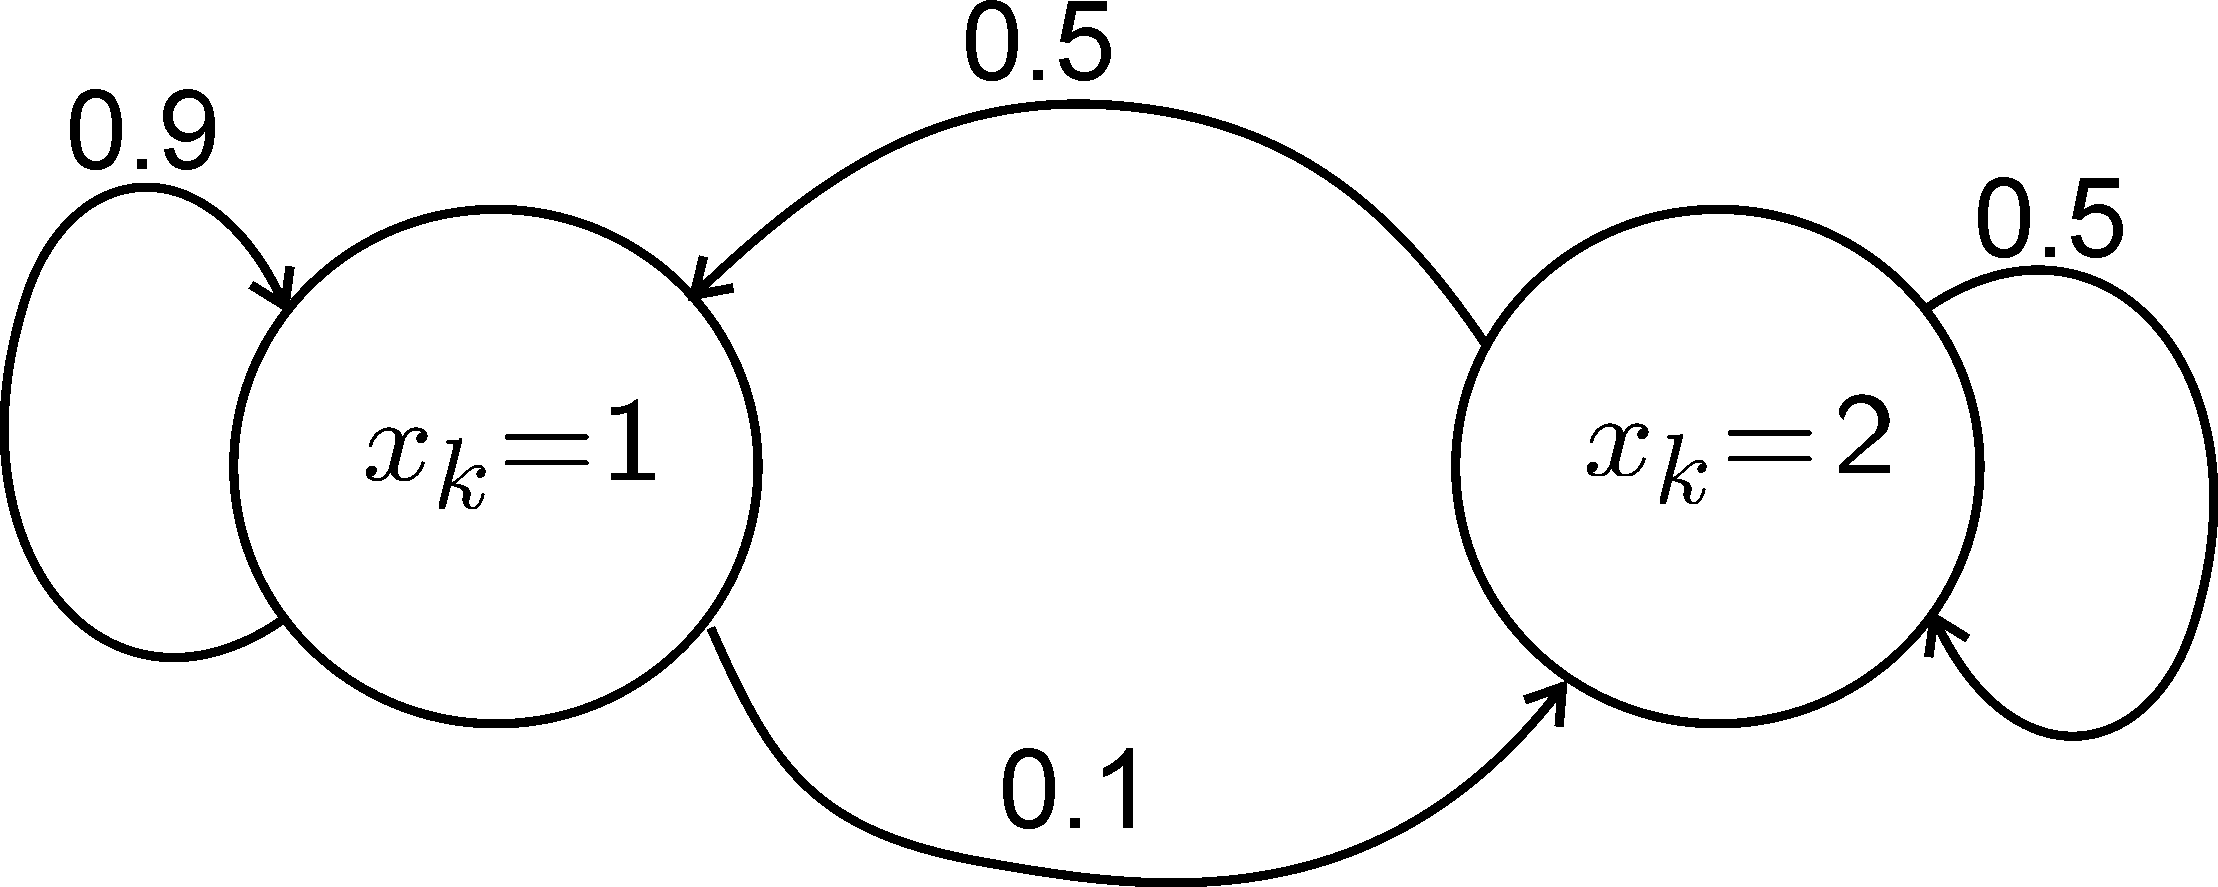
\includegraphics[bb=0bp 0bp 2218bp 887bp,clip,width=6cm]{filtre_markov_beau_temps}\caption{Markov chain describing the evolution of the weather in Brest }

\centering{}\label{fig:filtre_markov_beau_temps}
\end{figure}

1) We represent $\pi(x_{k})$ by a vector $\mathbf{p}_{k}$ of dimension
2. Using a Bayes filter, show that the evolution of $\mathbf{p}_{k}$
can be represented by a state equation of the form $\mathbf{p}_{k+1}=\mathbf{A}\cdot\mathbf{p}_{k}.$

2) At day $k$, the weather is sunny. What is the probability to be
sunny the day $k+\ell.$

3) What about this probability when $\ell$ tends to infinity?

\rule{0.95\columnwidth}{1pt}

\begin{Exercice} \label{ex:door:robot} Door robot$~$ \end{Exercice}

\textcolor{blue}{See the correction video at \href{https://youtu.be/J_0_-KTGpfM}{https://youtu.be/J\_0\_-KTGpfM}}

In this exercise, we illustrate the Bayes filter in a system with
a state $x\in\{0,1\}$. It corresponds \cite{Thrun05book} to a door
which can be closed ($x=0$) or open $(x=1)$ and an actuator to open
and close. The system has also a sensor to measure the state. The
input $u$, can be $u=-1,\,0$ or $1$ which mean 'close', 'do nothing'
or 'open'. The require input may fail (for instance, if someone stops
the door). We can represent the influence an $u$ on the state evolution
by the following table 
\[
\begin{tabular}{|c|c|c|c|}
\hline  \ensuremath{\pi(x_{k+1}|x_{k},u_{k})}  &  \ensuremath{u_{k}=-1,}  &  \ensuremath{u_{k}=0}  &  \ensuremath{u_{k}=1}\\
\hline  \ensuremath{x_{k}=0}  &  \ensuremath{\delta_{0}}  &  \ensuremath{\delta_{0}}  &  \ensuremath{0.2\ \delta_{0}+0.8\ \delta_{1}}\\
\hline  \ensuremath{x_{k}=1}  &  \ensuremath{0.8\ \delta_{0}+0.2\ \delta_{1}}  &  \ensuremath{\delta_{1}}  &  \ensuremath{\delta_{1}} 
\\\hline \end{tabular}
\]
For simplicity, the dependencies of the $\delta_{i}$ with respect
to $x_{k+1}$ is omitted. When we read in the table 
\[
\pi(x_{k+1}|x_{k}=0,u_{k}=1)=0.2\ \delta_{0}+0.8\ \delta_{1},
\]
it means that if $x_{k}=0$, there is a probability of $0.8$ to be
at state $1$ at time $k+1,$ if we apply the input $u_{k}=1$. The
sensor which gives us the state of the door is also uncertain. This
is represented by the following conditional density
\[
\begin{tabular}{|c|c|c|}
\hline  \ensuremath{\pi(y_{k}|x_{k})}  &  \ensuremath{x_{k}=0}  &  \ensuremath{x_{k}=1}\\
\hline  \ensuremath{y_{k}=0}  &  \ensuremath{0.8}  &  \ensuremath{0.4}\\
\hline  \ensuremath{y_{k}=1}  &  \ensuremath{0.2}  &  \ensuremath{0.6} 
\\\hline \end{tabular}
\]

The system can be represented by the graph of Figure \ref{fig:filtre_markov}.
\begin{figure}[H]
\centering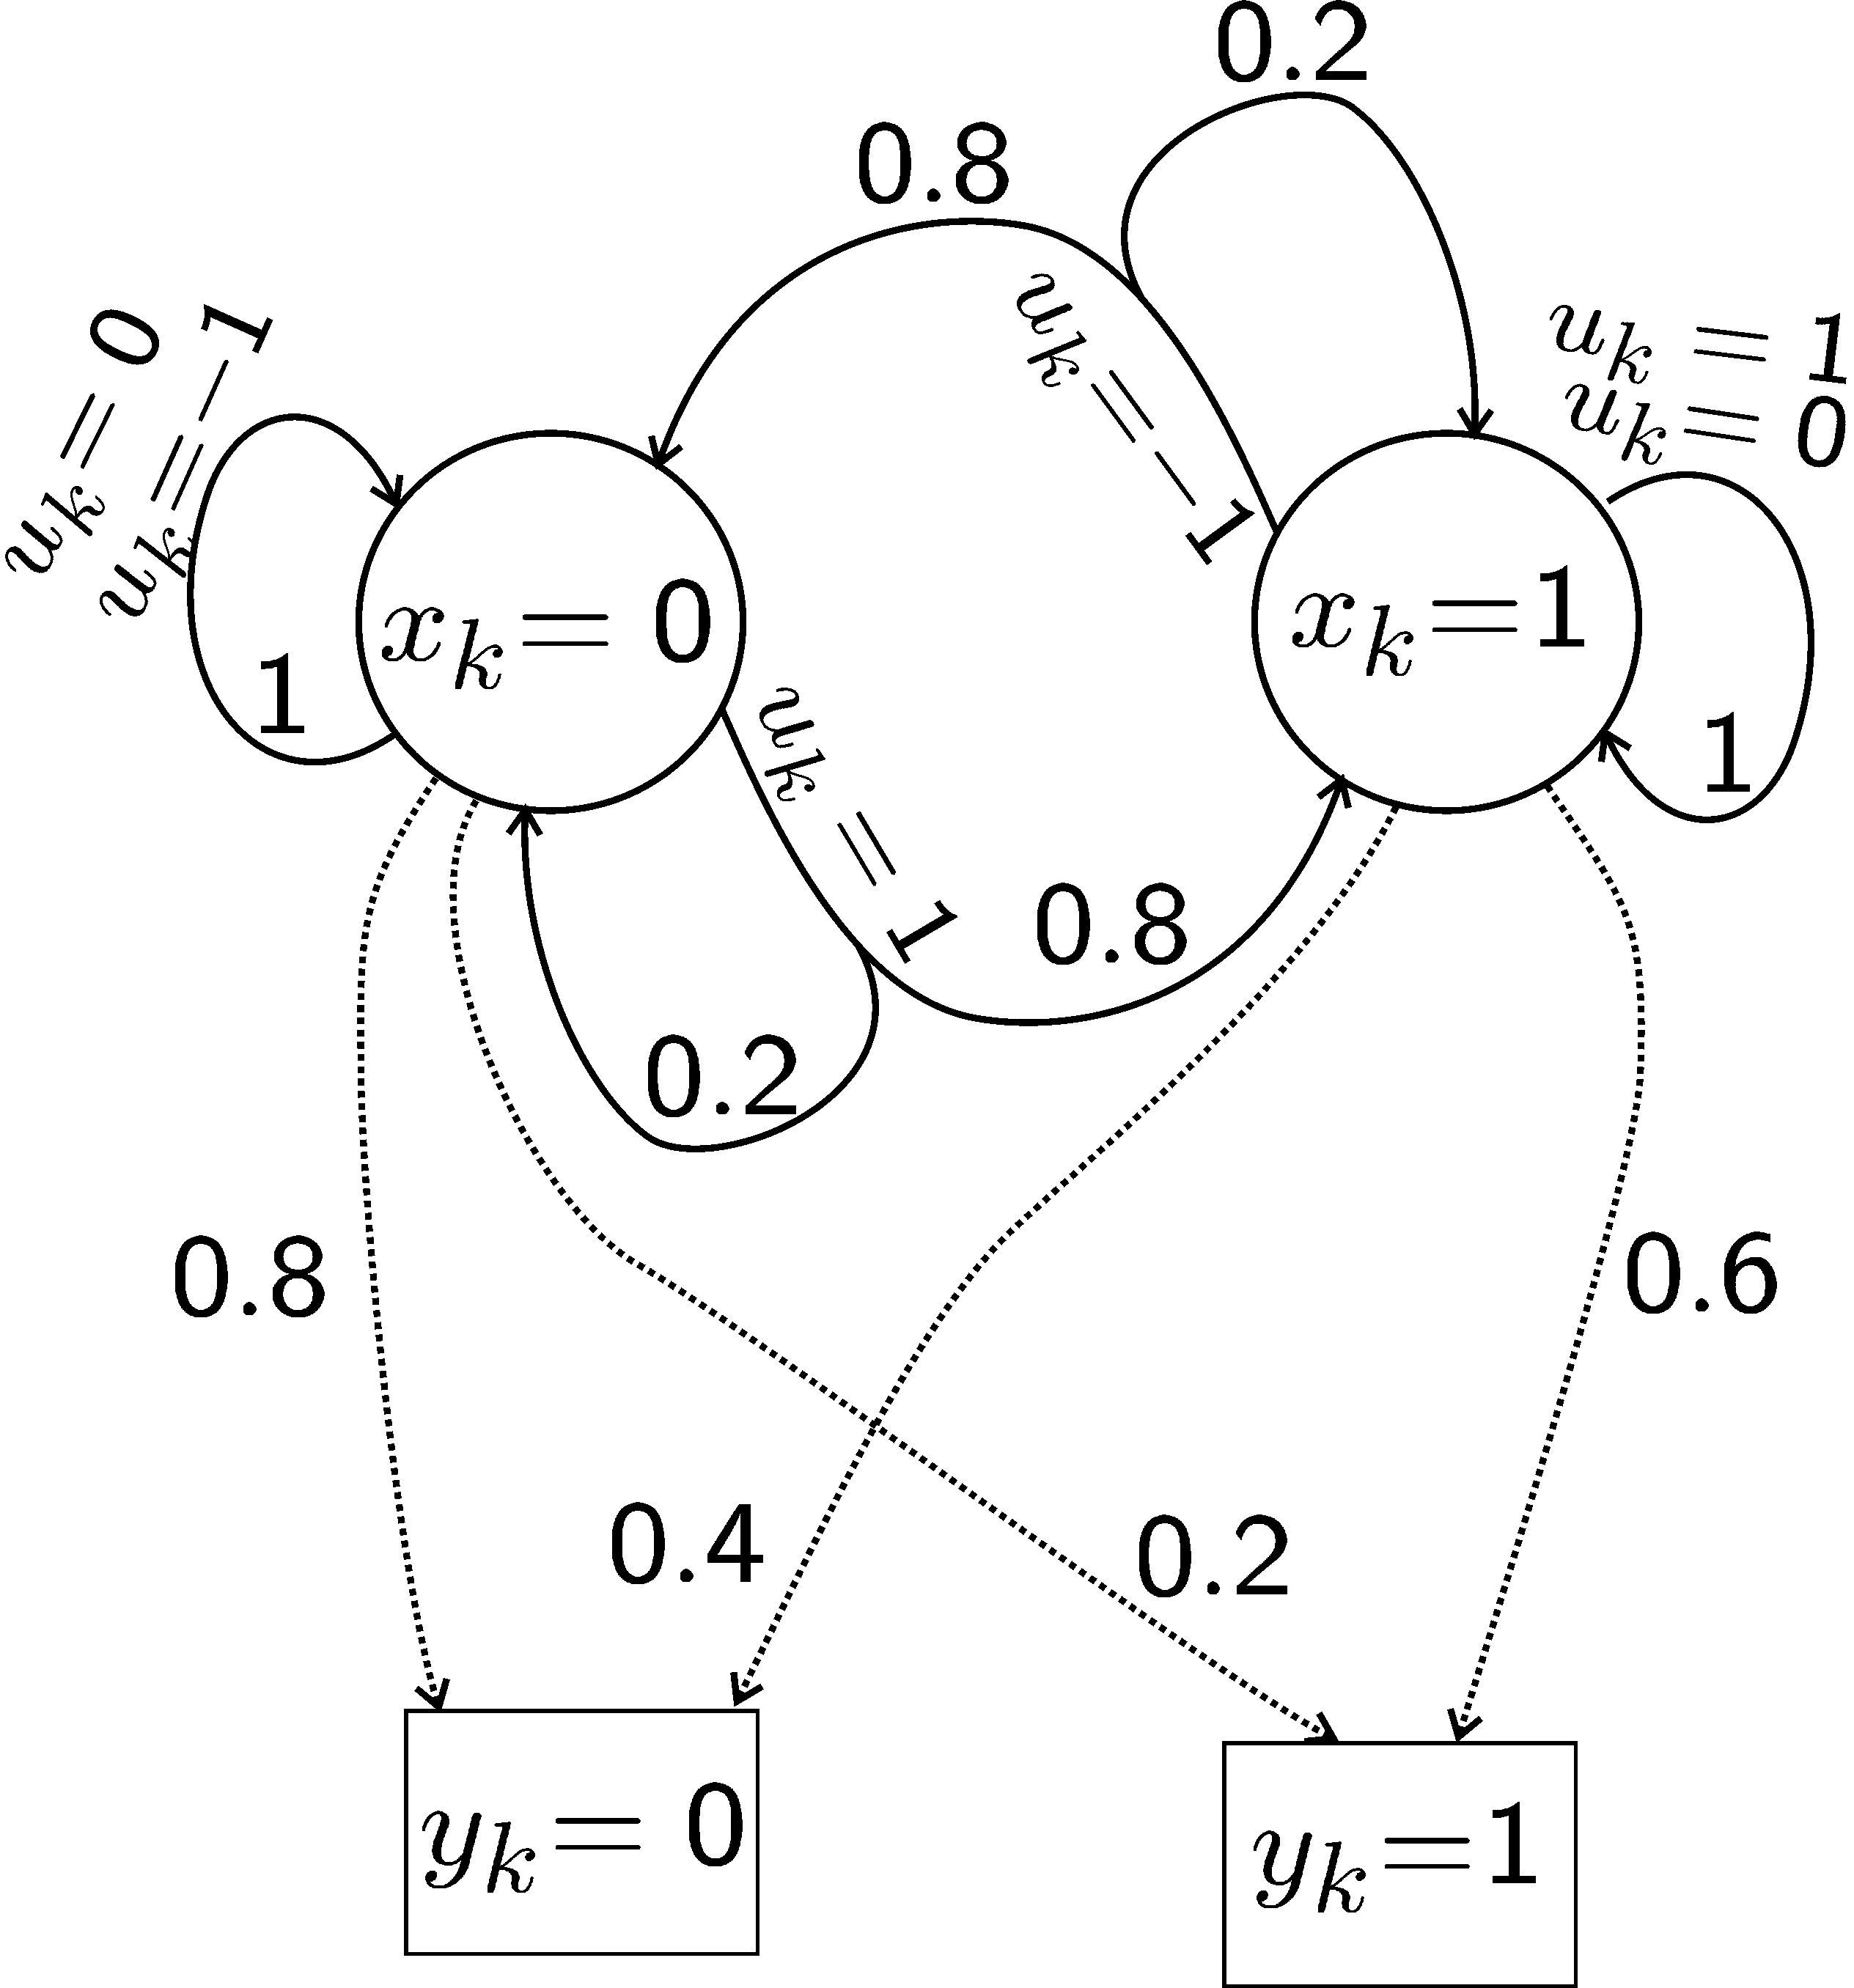
\includegraphics[bb=0bp 0bp 2529bp 2712bp,clip,width=6cm]{filtre_markov}\caption{Graph representing the evolution and the observation of the door robot}

\centering{}\label{fig:filtre_markov}
\end{figure}

1) Assume that the belief at time $k=0$ is given by bel$\left(x_{0}\right)=0.5\cdot\delta_{0}+0.5\cdot\delta_{1}$
and that $u_{0}=1$, compute pred$\left(x_{1}\right)$.

2) At time $1$ we measure $y_{1}=1$. Compute bel$\left(x_{1}\right).$

3) If $\mathbf{p}_{k}^{\text{pred}}$ and $\mathbf{p}_{k}^{\text{bel}}$
are the stochastic vectors associated to pred$\left(x_{k}\right)$
et bel$\left(x_{k}\right)$. Give the state equation for the Bayes
filter.

\rule{0.95\columnwidth}{1pt}

\begin{Exercice} \label{ex:filtre:bayesien:graphique} Robot in the
forest \end{Exercice}

\textcolor{blue}{See the correction video at \href{https://youtu.be/C443JFbwBvg}{https://youtu.be/C443JFbwBvg}}

The objective of this exercise if to give a graphical interpretation
of the Bayes filter. We recall that the Bayes filter is given by the
following equations
\[
\begin{array}{lll}
\text{pred}\left(\mathbf{x}_{k+1}\right) & = & \int\pi\left(\mathbf{x}_{k+1}|\mathbf{x}_{k},\mathbf{u}_{k}\right)\cdot\text{bel}\left(\mathbf{x}_{k}\right)\cdot d\mathbf{x}_{k}\\
\text{bel}\left(\mathbf{x}_{k}\right) & = & \frac{\pi(\mathbf{y}_{k}|\mathbf{x}_{k})\cdot\text{pred}\left(\mathbf{x}_{k}\right)}{\int\pi(\mathbf{y}_{k}|\mathbf{x}_{k})\cdot\text{pred}\left(\mathbf{x}_{k}\right)\cdot d\mathbf{x}_{k}}.
\end{array}
\]
Figure \ref{fig:filtre_bayes_robot} represents a robot with a scalar
state $x$ which corresponds to its position on a horizontal line.

\begin{figure}[H]
\centering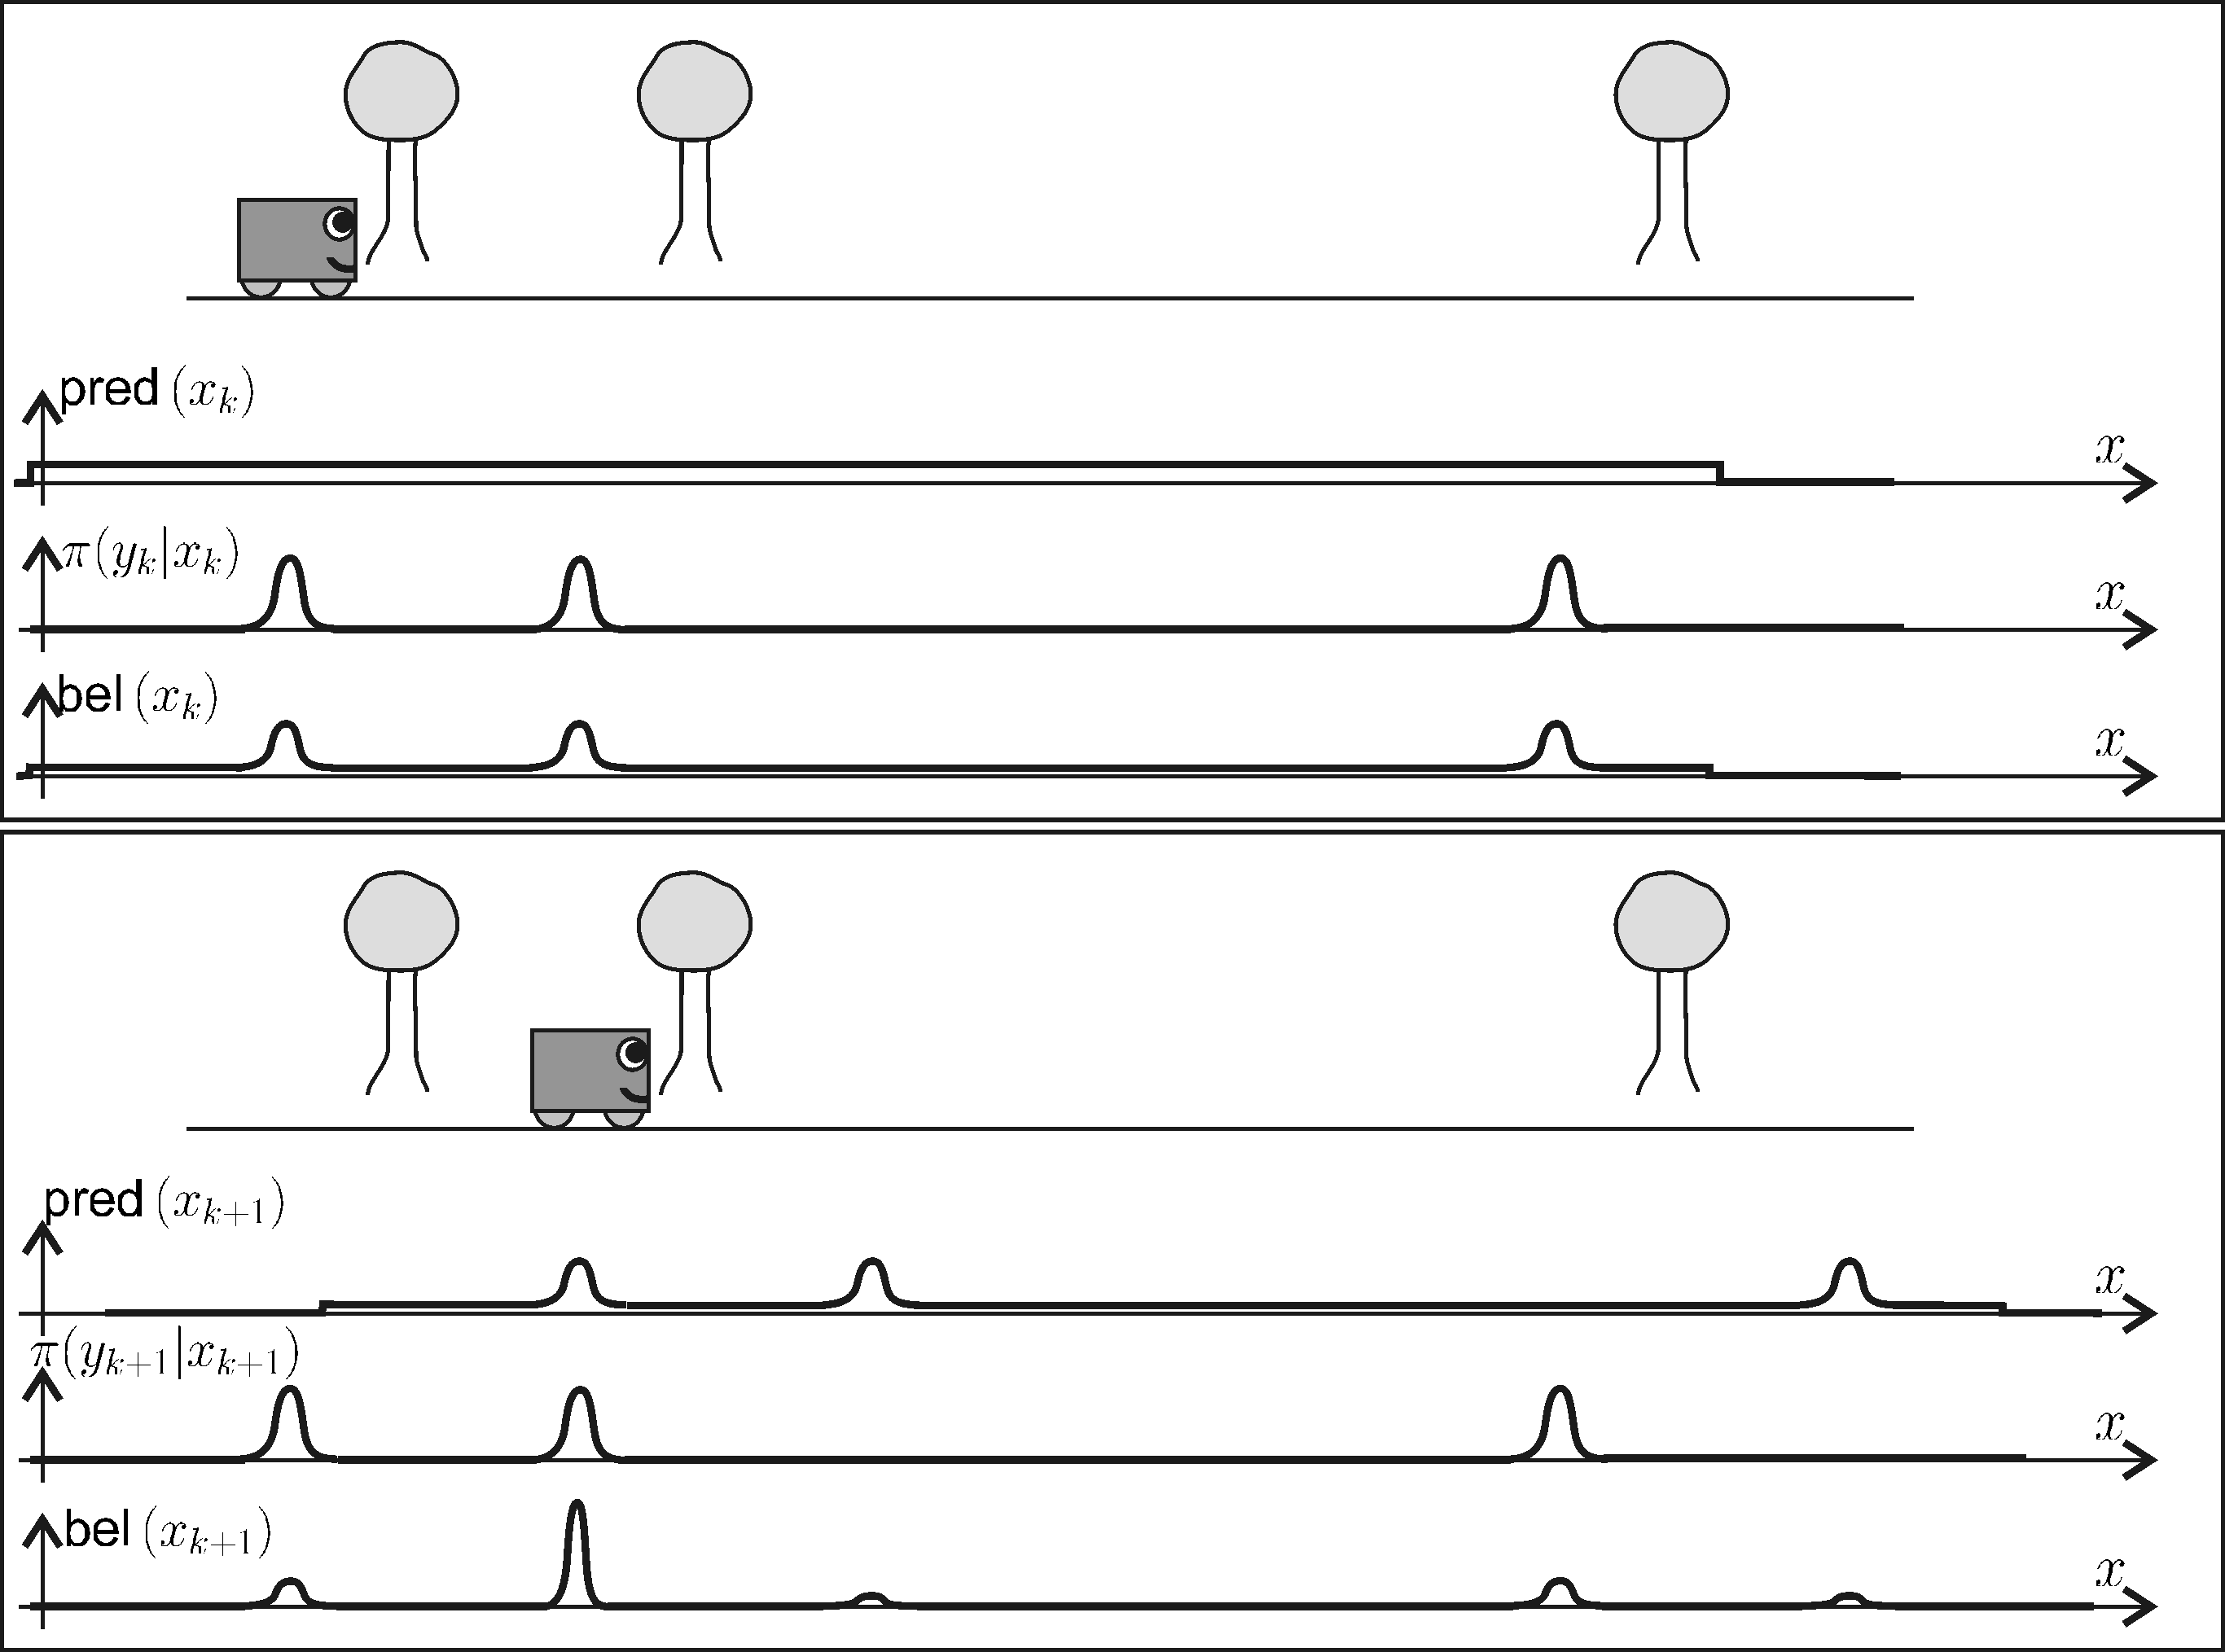
\includegraphics[bb=0bp 0bp 2732bp 2029bp,clip,width=12cm]{filtre_bayes_robot}\caption{Illustration of the Bayes filter}

\centering{}\label{fig:filtre_bayes_robot}
\end{figure}

\textbf{Step $k$}. We assume that at time $k$, we know from the
past the prediction pred$(x_{k})$, which is uniform on a large interval.
The robot knows that in its environment, there exists three trees
that are identical. Now, at time $k$, the robot sees a tree in front
of it. This corresponds the measurement $y_{k}$. It deduces the \emph{likelyhood}
$\pi\left(y_{k}|x_{k}\right)$ of $x$. The belief bel$\left(x_{k}\right)$
can thus be obtained simple multiplication of the density pred$\left(x_{k}\right)$
and the likelyhood $\pi\left(y_{k}|x_{k}\right)$, followed by a normalization.

\textbf{Step $k$}+1. The robot moves forward of few meters and the
counter $k$ increases by $1$. From the belief at time $k$ and the
knowledge of the motion, we can predict, via pred$(x_{k+1})$, the
state at time $k+1$. To get bel$\left(x_{k+1}\right)$ in the same
way as previously at time $k$.

\textbf{Step $k$}+2. Assume now that the robot moves forward again
of few meters but does not see any tree. Draw pred$(x_{k+2})$, $\pi\left(y_{k+2}|x_{k+2}\right)$
and bel$\left(x_{k+2}\right).$

\rule{0.95\columnwidth}{1pt}

\begin{Exercice} \label{ex:bayes:with:kalman} Bayes rule with Kalman
\end{Exercice}

\textcolor{blue}{See the correction video at \href{\%20https://youtu.be/aAM1nMhOKcw}{ https://youtu.be/aAM1nMhOKcw}}

Consider two Gaussian random variables $x\sim\mathcal{N}\left(1,1\right)$
and $b\sim\mathcal{N}\left(0,1\right)$, \emph{i.e.} the expectations
of $x$,$b$ are $\bar{x}=1$, $\bar{b}=0$ and the variances (\emph{i.e},
the covariance matrix in the scalar case) of $x$, $b$ are $\sigma_{x}^{2}=1$,
$\sigma_{b}^{2}=1$. 

1) Define $y=x+b$. Give the expression of probability density function
of $y$.

2) We collect the following measurement $y=3$. Using the correction
equations of the Kalman filter, compute the posterior density for
$x$.

3) Provide the link with the Bayes rule.

\rule{0.95\columnwidth}{1pt}

\begin{Exercice} \label{ex:kalman:smoother} Derivation of the Kalman
smoother \end{Exercice}

\textcolor{blue}{See the correction video at \href{https://youtu.be/aJKNEstmIfU}{https://youtu.be/aJKNEstmIfU}}

1) Consider two normal vectors $\mathbf{a}$ and $\mathbf{b}$. Show
that 
\begin{equation}
\left.\begin{array}{lcl}
\pi(\mathbf{a}) & = & \mathcal{N}\left(\mathbf{a}\left\Vert \mathbf{\hat{a}},\mathbf{\boldsymbol{\Gamma}}_{\mathbf{a}}\right.\right)\\
\pi(\mathbf{b}|\mathbf{a}) & = & \mathcal{N}\left(\mathbf{b}\left\Vert \mathbf{J}\mathbf{a}+\mathbf{u},\mathbf{R}\right.\right)
\end{array}\right\} \,\,\,\,\,\Longrightarrow\,\,\,\,\pi(\mathbf{b})=\mathcal{N}\left(\mathbf{b}\left\Vert \mathbf{J}\mathbf{\hat{a}}+\mathbf{u},\mathbf{R}+\mathbf{J}\cdot\mathbf{\boldsymbol{\Gamma}}_{\mathbf{a}}\cdot\mathbf{J}^{\text{T}}\right.\right).\label{eq:lemma:smoother}
\end{equation}

2) Consider a linear discrete time system described by the state equation.
\[
\left\{ \begin{array}{ccl}
\mathbf{x}_{k+1} & = & \mathbf{A}_{k}\mathbf{x}_{k}+\mathbf{u}_{k}+\mathbf{\boldsymbol{\alpha}}_{k}\\
\mathbf{y}_{k} & = & \mathbf{C}_{k}\mathbf{x}_{k}+\mathbf{\boldsymbol{\beta}}_{k}
\end{array}\right.
\]
where $\mathbf{\boldsymbol{\alpha}}_{k}$ and $\mathbf{\boldsymbol{\beta}}_{k}$
are Gaussian, white and independent. Using the equations of the Kalman
filter, show that 
\begin{equation}
\begin{array}{ccc}
\pi\left(\mathbf{x}_{k}|\mathbf{x}_{k+1},\mathbf{y}_{0:N}\right) & = & \mathcal{N}\left(\mathbf{x}_{k}\left\Vert \mathbf{\hat{x}}_{k|k}+\,\mathbf{J}_{k}\left(\mathbf{x}_{k+1}-\mathbf{\hat{x}}_{k+1|k}\right),\mathbf{\boldsymbol{\mathbf{\Gamma}}}_{k|k}-\mathbf{J}_{k}\cdot\mathbf{\boldsymbol{\boldsymbol{\Gamma}}}_{k+1|k}\cdot\mathbf{J}_{k}^{T}\right.\right)\end{array}\label{eq:pi:xk:xk1:y0N}
\end{equation}
where
\[
\mathbf{J}_{k}=\mathbf{\boldsymbol{\Gamma}}_{k|k}\cdot\mathbf{A}_{k}^{T}\cdot\mathbf{\boldsymbol{\boldsymbol{\Gamma}}}_{k+1|k}^{-1}.
\]

3) From the two previous questions, show that the smoothing density
is
\[
\text{back}\left(\mathbf{x}_{k}\right)=\pi\left(\mathbf{x}_{k}|\mathbf{y}_{0:N}\right)=\mathcal{N}\left(\mathbf{x}_{k}\left\Vert \mathbf{\hat{x}}_{k|N},\mathbf{\mathbf{\boldsymbol{\Gamma}}}_{k|N}\right.\right)
\]
where
\[
\begin{array}{lll}
\mathbf{\hat{x}}_{k|N} & = & \mathbf{\hat{x}}_{k|k}+\mathbf{J}_{k}\cdot\left(\mathbf{\hat{x}}_{k+1|N}-\mathbf{\hat{x}}_{k+1|k}\right)\\
\mathbf{\boldsymbol{\boldsymbol{\Gamma}}}_{k|N} & = & \boldsymbol{\boldsymbol{\Gamma}}_{k|k}-\mathbf{J}_{k}\cdot\left(\mathbf{\boldsymbol{\boldsymbol{\Gamma}}}_{k+1|k}-\mathbf{\boldsymbol{\boldsymbol{\Gamma}}}_{k+1|N}\right)\cdot\mathbf{J}_{k}^{\text{T}}.
\end{array}
\]

\rule{0.95\columnwidth}{1pt}

\begin{Exercice} \label{ex:kalman:slam} SLAM$~$ \end{Exercice}

\textcolor{blue}{See the correction video at \href{http://youtu.be/KHkP4vf_th0}{http://youtu.be/KHkP4vf\_th0}}

The \emph{Redermor} (underwater robot built by GESMA, Brest) performed
a two-hour mission in the Douarnenez bay (see Figure \ref{fig:redermor}).
During its mission, it collected data from its inertial unit (which
gives us the Euler angles $\phi,\theta,\psi$), its Doppler log (which
gives us the robot's speed $\mathbf{v}_{r}$ in the robot's coordinate
system), its pressure sensor (which gives us the robot's depth $p_{z}$)
and its altitude sensor (sonar that gives us the altitude $a$), with
a sampling period of $dt=0.1~\sec$. This data can be found in the
file \texttt{slam\_data.txt}. The file is composed of 59 996 lines
(one line per sampling period) and 9 columns which are respectively:
\[
\left(t,\varphi,\theta,\psi,v_{x},v_{y},v_{z},p_{z},a\right)
\]
where $p_{z}$ is the depth of the robot and $a$ is its altitude
(\emph{i.e.}, its distance to the seabed).

\begin{figure}[h]
\centering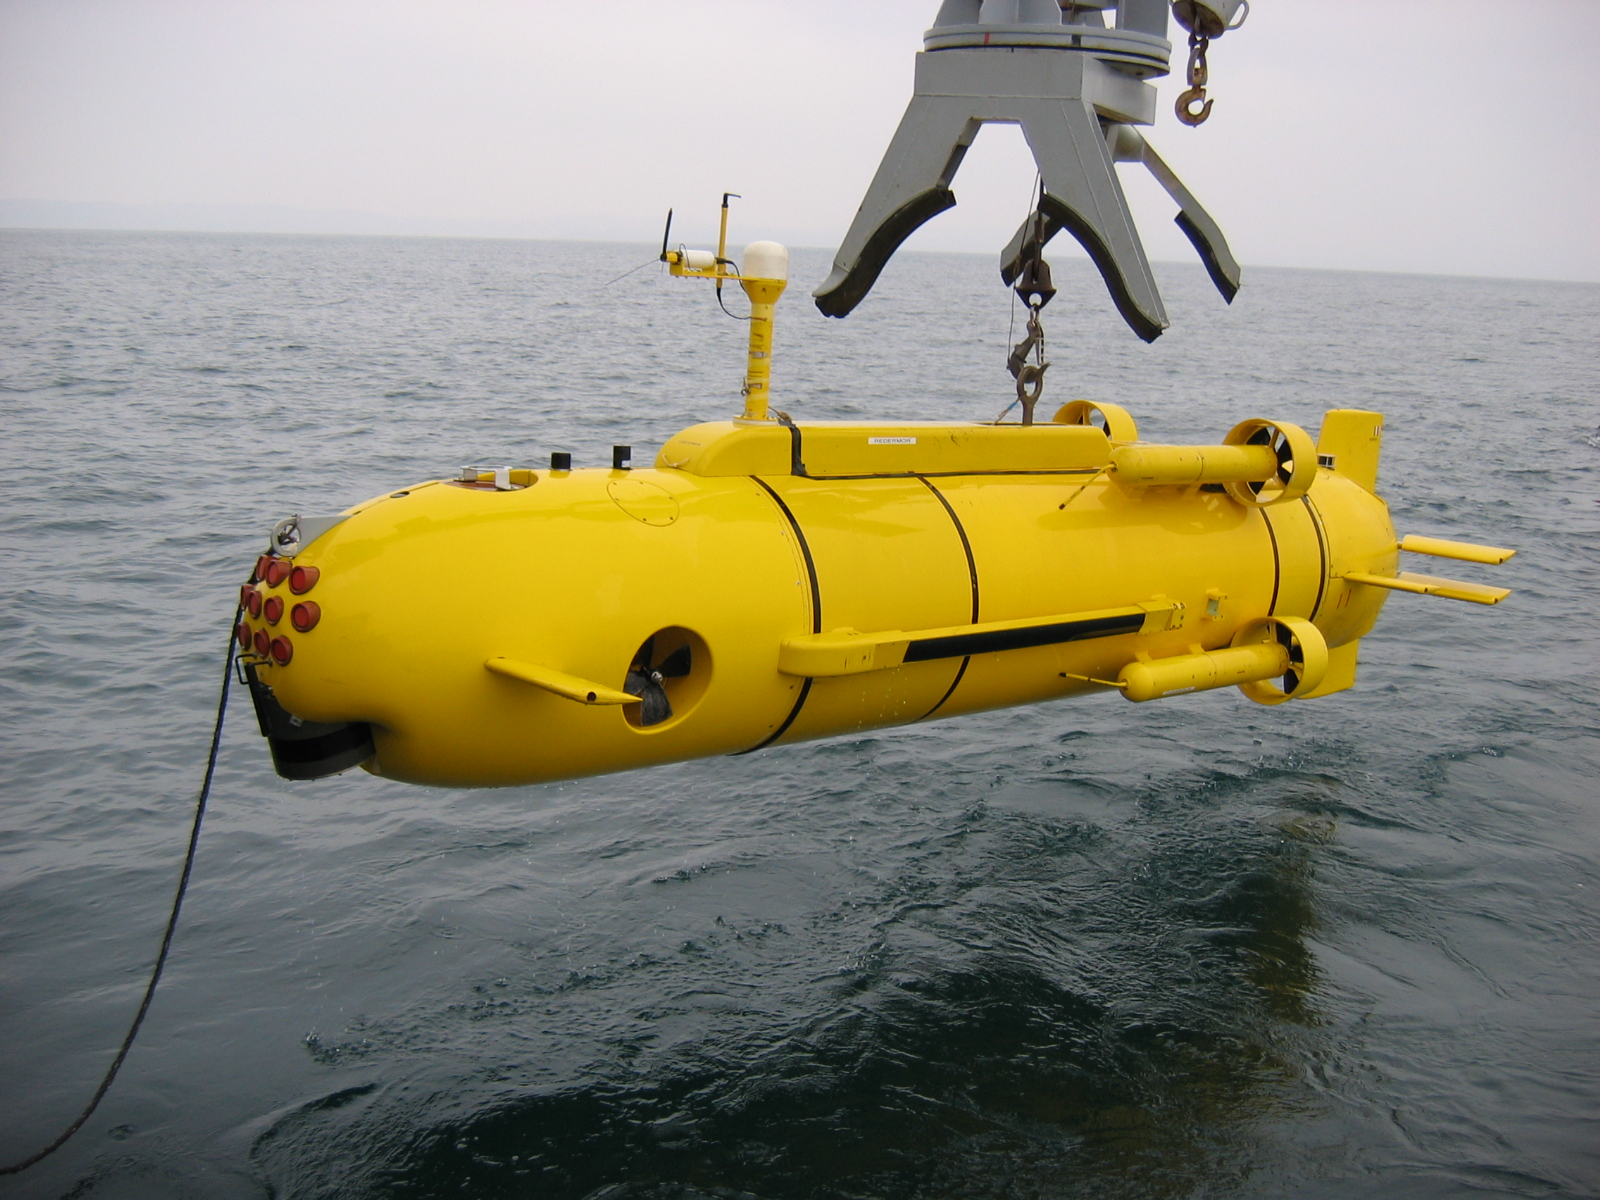
\includegraphics[width=0.7\textwidth]{AUVair2}\caption{The \emph{Redermor}, built by GESMA (Groupe d'Etude Sous-Marine de
l'Atlantique), right before diving into the water}

\label{fig:redermor}
\end{figure}

1) Given that the robot started from a position $\mathbf{p}=\left(0,0,0\right)$,
at time $t=0$, and using an Euler method, deduce an estimation for
the path. Use for this the state equation: 
\[
\mathbf{\dot{p}}(t)=\mathbf{R}(\varphi\left(t\right),\theta\left(t\right),\psi\left(t\right))\cdot\mathbf{v}_{r}(t)
\]
with $\mathbf{R}(\varphi,\theta,\psi)$ the Euler matrix given by:
\[
\mathbf{R}(\varphi,\theta,\psi)=\left(\begin{array}{ccc}
\cos\psi & -\sin\psi & 0\\
\sin\psi & \cos\psi & 0\\
0 & 0 & 1
\end{array}\right)\left(\begin{array}{ccc}
\cos\theta & 0 & \sin\theta\\
0 & 1 & 0\\
-\sin\theta & 0 & \cos\theta
\end{array}\right)\left(\begin{array}{ccc}
1 & 0 & 0\\
0 & \cos\varphi & -\sin\varphi\\
0 & \sin\varphi & \cos\varphi
\end{array}\right)
\]
2) The angles $\varphi,\theta,\psi$ are measured with a standard
deviation of $\left(2\times10^{-4},2\times10^{-4},\!\!\!\right.$
$\left.5\times10^{-3}\right)$. The components of $\mathbf{v}_{r}$
are measured every $dt$ seconds with a variance of $\sigma_{v}^{2}\!=\!1m^{2}s^{-2}$.
We may assume that the robot satisfies the equation: 
\[
\mathbf{p}_{k+1}=\mathbf{p}_{k}+\left(dt\cdot\mathbf{R}(k)\right)\cdot\mathbf{\bar{v}}_{r}(k)+\mathbf{\boldsymbol{\alpha}}_{k}
\]
where $\mathbf{\boldsymbol{\alpha}}_{k}$ is a white noise and $\mathbf{\bar{v}}_{r}(k)$
is a measurement of the average speed over the corresponding sampling
period. Show that a realistic covariance matrix for $\mathbf{\boldsymbol{\alpha}}_{k}$
is: 
\[
\mathbf{\boldsymbol{\Gamma}}_{\mathbf{\boldsymbol{\alpha}}}=dt^{2}\sigma_{v}^{2}\cdot\left(\begin{array}{lclcl}
1 &  & 0 &  & 0\\
0 &  & 1 &  & 0\\
0 &  & 0 &  & 1
\end{array}\right).
\]
\textbf{Remark}. We are not in the situation described in Section
\ref{sec:Kalman-Bucy} or in Exercise \ref{ex:brownien} where the
covariance for the state noise should have the same order as $\frac{1}{dt}$
. Here, our system in not a discretisation of a continuous random
process, the behavior of which should be independent of $dt$. On
the contrary, $dt$ is a sampling time of the velocity sensor. Smaller
is $dt$, more accurate will be the integration.

3) Using the Kalman filter as predictor, calculate the precision with
which the robot knows its position at each moment $t=k\cdot dt$.
Give, in function of $t$, the standard deviation of the error over
the position. What will this become after an hour ? After two hours
? Verify your calculations experimentally by implementing a Kalman
predictor.

4) During its mission, the robot may detect several landmarks with
its lateral sonar (here these will be mines). When the robot detects
a landmark, it will be on its right side and in a plane perpendicular
to the robot. The seabed is assumed to be flat and horizontal. The
following table shows the detection times, the numbers $i$ of the
landmarks and the distance $r_{i}$ between the robot and the landmark:
\[
\begin{tabular}{|c|c|c|c|c|c|c|c|c|c|c|c|c|}
\hline  \ensuremath{t}  &  \ensuremath{1054}  &  \ensuremath{1092}  &  \ensuremath{1374}  &  \ensuremath{1748}  &  \ensuremath{3038}  &  \ensuremath{3688}  &  \ensuremath{4024}  &  \ensuremath{4817}  &  \ensuremath{5172}  &  \ensuremath{5232}  &  \ensuremath{5279}  &  \ensuremath{5688}\\
\hline  \ensuremath{i}  &  \ensuremath{1}  &  \ensuremath{2}  &  \ensuremath{1}  &  \ensuremath{0}  &  \ensuremath{1}  &  \ensuremath{5}  &  \ensuremath{4}  &  \ensuremath{3}  &  \ensuremath{3}  &  \ensuremath{4}  &  \ensuremath{5}  &  \ensuremath{1}\\
\hline  \ensuremath{r_{i}(t)}  &  \ensuremath{52.4}  &  \ensuremath{12.47}  &  \ensuremath{54.4}  &  \ensuremath{52.7}  &  \ensuremath{27.73}  &  \ensuremath{27.0}  &  \ensuremath{37.9}  &  \ensuremath{36.7}  &  \ensuremath{37.37}  &  \ensuremath{31.03}  &  \ensuremath{33.5}  &  \ensuremath{15.05} 
\\\hline \end{tabular}
\]
SLAM (\emph{Simultaneous Localization And Mapping}) seeks to use these
repeated detections to improve the precision of the estimation of
its path. For this, we form a large state vector $\mathbf{x}$, of
dimension $3+2\cdot6=15$ that contains the position of the robot
$\mathbf{p}$ as well as the vector $\mathbf{q}$ of dimension 12
containing the coordinates (as $x$ and $y$) of the six landmarks.
Let us note that since the landmarks are immobile, we have $\mathbf{\dot{q}=0}$.
Give the function $\left(\mathbf{y},\mathbf{C}_{k},\boldsymbol{\Gamma}_{\boldsymbol{\beta}}\right)=\mathbf{g}\left(k\right)$
that corresponds to the observation. This function returns the measurement
vector $\mathbf{y}$, the matrix $\mathbf{C}(k)$ and the covariance
matrix of the measurement noise. As for the standard deviation of
the measurement noise $\mathbf{\beta}_{k}$, we will take $0.1$ for
that of the depth and $1$ for that of the robot-landmark distance.

5) Using a Kalman filter, find the position of the landmarks together
with the associated uncertainty. Show how the robot was able to readjust
its position.

6) Use the Kalman smoother to improve the precision over the landmark
positions by taking into account the past as well as the future.

\rule{0.95\columnwidth}{1pt}

\begin{Exercice} \label{ex:particle:filter} Particle filter \end{Exercice}

\textcolor{blue}{See the correction video at \href{https://youtu.be/xKaXff5yzwI}{https://youtu.be/xKaXff5yzwI}}

We consider a robot at position $\mathbf{x}=(x_{1},x_{2})$ that has
to be localized. The robot is equipped with a compass, so that we
can assume that its heading $\theta$ is known. We describe the evolution
of the robot by the relation
\[
\mathbf{x}_{k+1}=\mathbf{x}_{k}+dt\cdot\left(\begin{array}{l}
\cos\theta_{k}\\
\sin\theta_{k}
\end{array}\right)+\boldsymbol{\alpha}_{k}
\]
where the sampling time is taken as $dt$, where $\boldsymbol{\alpha}_{k}$
is the state noise. The covariance matrix for $\boldsymbol{\alpha}_{k}$
is taken as 
\[
\boldsymbol{\Gamma}_{\boldsymbol{\alpha}}=0.1\cdot\left(\begin{array}{cc}
dt & 0\\
0 & dt
\end{array}\right).
\]
In the environment, we have 3 landmarks at position: 

\noindent\begin{minipage}[t]{1\columnwidth}%
\begin{center}
\begin{tabular}{|c|c|c|c|}
\hline 
$j$ & $1$ & $2$ & $3$\tabularnewline
\hline 
$\ensuremath{\mathbf{m}}\ensuremath{(j)}$ & $\left(\begin{array}{c}
3\\
8
\end{array}\right)$ & $\left(\begin{array}{c}
2\\
6
\end{array}\right)$ & $\left(\begin{array}{c}
4\\
11
\end{array}\right)$\tabularnewline
\hline 
\end{tabular}
\par\end{center}%
\end{minipage}

At each time $t_{k}=k\cdot dt$, the robot measures its distance to
each landmark with an error. The corresponding observation equation
is
\[
\mathbf{y}_{k}=\left(\begin{array}{c}
\|\mathbf{x}-\mathbf{m}(1)\|\\
\|\mathbf{x}-\mathbf{m}(2)\|\\
\|\mathbf{x}-\mathbf{m}(3)\|
\end{array}\right)+\boldsymbol{\beta}_{k}
\]
where the components for $\boldsymbol{\beta}_{k}$ are all independent
with a variance of 1. All noises $\boldsymbol{\alpha}_{k}$, $\boldsymbol{\beta}_{k}$
are white, stationary, centered and Gaussian. In this exercise, we
want to estimate the probability density functions
\[
\begin{array}{lll}
\text{pred}(\mathbf{x}_{k}) & = & \pi(\mathbf{x}_{k}|\mathbf{y}_{0:k-1})\\
\text{bel}(\mathbf{x}_{k}) & = & \pi(\mathbf{x}_{k}|\mathbf{y}_{0:k}).
\end{array}
\]
 by a weighted set of $N$ samples, called the \emph{cloud}, 
\[
(\mathcal{P},\mathcal{W})(k)=\left\{ (w_{k}^{(1)},\mathbf{x}_{k}^{(1)}),\dots,(w_{k}^{(N)},\mathbf{x}_{k}^{(N)})\right\} ,
\]
where $\sum_{\ell}w_{k}^{(\ell)}=1.$ The weight $w_{k}^{(\ell)}$
is an approximation of the probability for the state $\mathbf{x}(k)$
to be equal to $\mathbf{x}_{k}^{(\ell)}$. We define the set of particles
$\mathcal{P}$ and the set of of weights $\mathcal{W}$ as
\[
\begin{array}{ccc}
\mathcal{P} & = & \left\{ \mathbf{x}_{k}^{(1)},\dots,\mathbf{x}_{k}^{(N)}\right\} \\
\mathcal{W} & = & \left\{ w_{k}^{(1)},\dots,w_{k}^{(N)}\right\} .
\end{array}
\]

For the simulations, we will take $\mathbf{x}(0)=(0,0),$ $\theta(t)=0.2\cdot t$,
$t_{k}=k\cdot dt$, $dt=0.1$ and $N=2000$. 

1) Assume that at time $k=0$, we know that $\text{pred}(\mathbf{x}_{k})$
is uniformly distributed inside the box $[-15,15]\times[-15,15]$.
Generate the corresponding cloud $(\mathcal{P},\mathcal{W})$ and
draw the particles with a width proportional to their weights. 

2) At time $t=0$, the robot at position $\mathbf{x}(0)$ measures
$\mathbf{y}_{0}$ that you should generate from the observation equation.
Using the rule
\[
\text{bel}(\mathbf{x}_{k})=\frac{\pi(\mathbf{y}_{k}|\mathbf{x}_{k})\cdot\text{pred}(\mathbf{x}_{k})}{\pi(\mathbf{y}_{k}|\mathbf{y}_{0:k-1})}
\]
update the weights $\mathcal{W}$ to get an estimation of $\text{bel}(\mathbf{x}_{0})$.
An illustration of the cloud you should obtain is given by Figure
\ref{fig:particle1}(b).

3) Generate a \emph{resampled} cloud $(\mathcal{P}',\mathcal{W}')$
from the previous one $(\mathcal{P},\mathcal{W})$ which also represents
$\text{bel}(\mathbf{x}_{0})$. Now, with the resampled cloud, all
weights should be equal to $\frac{1}{N}$, as illustrated by Figure
\ref{fig:particle1}(c).

4) Using the prediction equation 
\[
\text{pred}(\mathbf{x}_{k+1})=\int\pi(\mathbf{x}_{k+1}|\mathbf{x}_{k})\cdot\text{bel}(\mathbf{x}_{k})\cdot d\mathbf{x}_{k}
\]
Generate a cloud $(\mathcal{P}'',\mathcal{W}'')$ which approximates
$\text{pred}(\mathbf{x}_{1})$ from the resampled cloud $(\mathcal{P}',\mathcal{W}')$.
See Figure \ref{fig:particle1}(d). 

5) Write a program which simulates the robot for $t\in[0,5]$. Propose
a particle filter for localizing the robot. Show the evolution of
the cloud associated with $\text{pred}(\mathbf{x}_{k})$. 

\begin{figure}[H]
\centering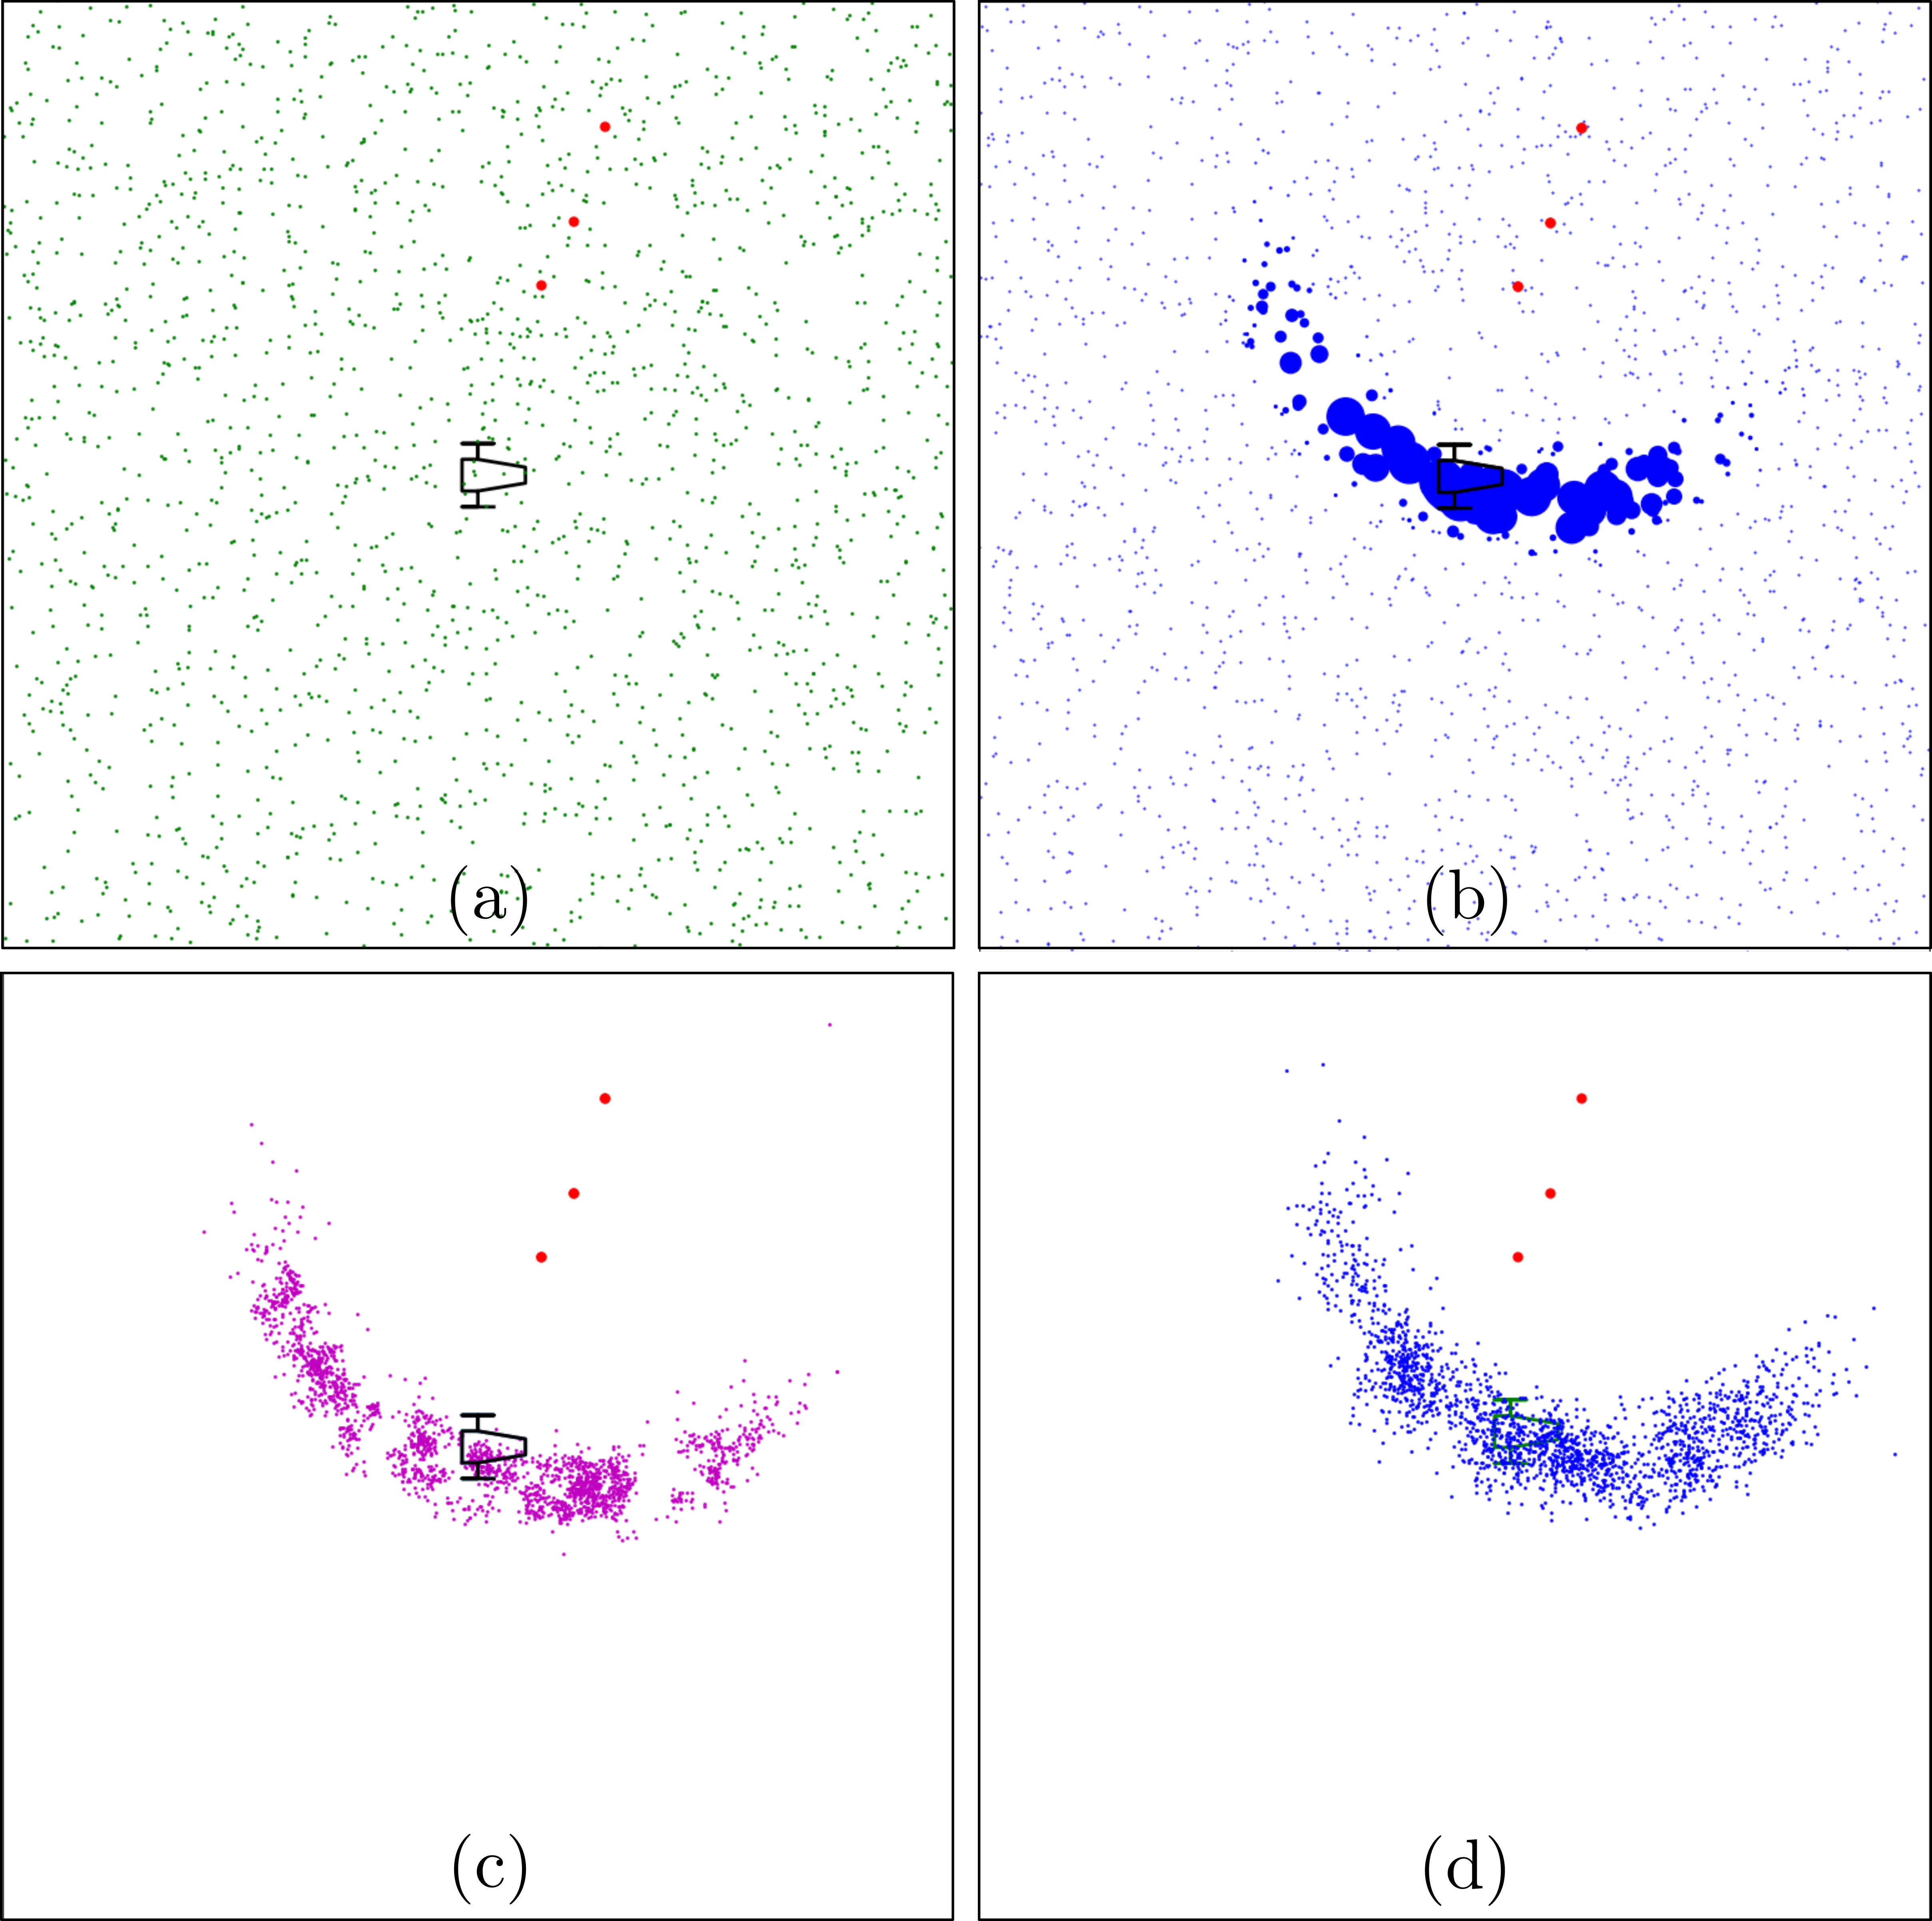
\includegraphics[width=12cm]{particle1} \caption{(a) $\text{pred}(\mathbf{x}_{0})$; (b) $\text{bel}(\mathbf{x}_{0})$:
the particles have different weights; (c) $\text{bel}(\mathbf{x}_{0})$
after resampling: all particles have the same weight; (d) $\text{pred}(\mathbf{x}_{1})$
: the robot has moved forward}

\label{fig:particle1}
\end{figure}

\begin{verbatim}

\end{verbatim}
\bigskip{}

\bigskip{}

\bibliographystyle{unsrt}
\bibliography{interval}

\end{document}
